\documentclass[%
% PARA ESCOLHER O ESTILO TIRE O SIMBOLO %(COMENTÁRIO)
%SemVinculoColorido,
%SemFormatacaoCapitulo,
%SemFolhaAprovacao,
%SemImagens,
%CitacaoNumerica, %% o padrão é citação tipo autor-data
%PublicacaoDissOuTese, %% (é também o "default") com ficha catal. e folha de aprovação em branco. Caso tenha lista de símbolos e lista de siglas e abreviaturas retirar os comentários dos arquivos siglas.tex e abreviaturasesiglas.tex. Retirar também os comentários indicados nesse arquivo, nos includes
%PublicacaoArtigoOuRelatorio, %% texto sequencial, sem quebra de páginas nem folhas em branco
PublicacaoProposta, %% igual tese/dissertação, mas sem ficha catal. e fol. de aprov.
%PublicacaoLivro, %% com capítulos
%PublicacaoLivro,SemFormatacaoCapitulo, %% sem capítulos
english,portuguese %% para os documentos em Português com abstract.tex em Inglês
%portuguese,english %% para os documentos em Inglês com abstract.tex em Português
,LogoINPE% comentar essa linha para fazer aparecer o logo do Governo
,CCBYNC	% as opções de licença são: CCBY, CCBYSA, CCBYND, CCBYNC, CCBYNCSA, CCBYNCND, GPLv3 e INPECopyright
]{tdiinpe}

% PARA EXIBIR EM ARIAL TIRAR O COMENTÁRIO DAS DUAS LINHAS SEGUINTES
%\renewcommand{\rmdefault}{phv} % Arial
%\renewcommand{\sfdefault}{phv} % Arial

% PARA PUBLICAÇÕES EM INGLÊS:
% renomear o arquivo: abnt-alf.bst para abnt-alfportuguese.bst
% renomear o arquivo: abnt-alfenglish.bst para abnt-alf.bst

% Pacotes já previamente carregados:      %
% ifthen,calc,graphicx,color,inputenc,babel,hyphenat,array,setspace,
% bigdelim,multirow,supertabular,tabularx,longtable,lastpage,lscape,
% rotate,caption2,amsmath,amssymb,amsthm,subfigure,tocloft,makeidx, 
% eso-pic,calligra,hyperref,ae,fontenc                               

%\watermark{Revisão No. ##} 

% Engana o pacote tcolorbox no carregamento do inputenc
% REF: https://tex.stackexchange.com/questions/370262/how-to-adapt-tcolorbox-with-xelatex
\makeatletter\@namedef{ver@inputenc.sty}{}\makeatother

% Pacotes Extras
\usepackage{rotating}
\usepackage{dsfont}
\usepackage{comment}
\usepackage{xcolor}
\usepackage{xcolor-material}
\usepackage{xcolor-solarized}
\usepackage[cachedir=.mintedcache]{minted}
\usemintedstyle{material}
\usepackage{multicol}
\usepackage{listings}
\usepackage{ulem}
\usepackage{cancel}
\usepackage{lipsum} 
\usepackage{graphicx}
\usepackage{pstricks}
\usepackage{pst-plot}
\usepackage{pst-3dplot}
\usepackage{booktabs}
\usepackage{wrapfig}
\usepackage{chngcntr}
\counterwithin*{footnote}{section}
\usepackage{metalogo}
\usepackage{enumitem}
%\usepackage{caption}
%\usepackage{subcaption}
\usepackage{subfig}
\usepackage[most]{tcolorbox}
\tcbuselibrary{breakable}
\tcbuselibrary{minted}
\usetikzlibrary{decorations.pathmorphing} 
\tcbuselibrary{skins}
\usepackage{setspace}
\PassOptionsToPackage{hyphens}{url}\usepackage{hyperref}
\usepackage{xspace}
\usepackage{lscape}
\usepackage{pdfpages}


%%%%%%%%%%%%%%%%%%%CAPA%%%%%%%%%%%%%%%%%%%%%%%%%%%%%%%%
%\serieinpe{INPE-NNNNN-TDI/NNNN} %% n\~{a}o mais usado

\titulo{Escrever o t\'{i}tulo no idioma em que foi escrito a publicaç\~{a}o}
\title{Escrever o t\'{i}tulo em Ingl\^{e}s para publicaç\~{o}es escritas em Portugu\^{e}s e em Portugu\^{e}s para publicaç\~{o}es escritas em Ingl\^{e}s} %% 
\author{Nome Completo do Autor} %% coloque o nome do(s) autor(es)
\descriccao{Tese de Doutorado ou Dissertaç\~{a}o de Mestrado do Curso de P\'{o}s-Graduaç\~{a}o em Nome do Curso, orientada pelo(a) Dr(a). Nome do Orientador(a), aprovada em dd de m\^{e}s por extenso de aaaa.}
\repositorio{aa/bb/cc/dd} %% reposit\'{o}rio onde est\'{a} depositado este documento - na omiss\~{a}o, ser\'{a} preenchido pelo SID
\tipoDaPublicacao{TDI}	%% tipo da publicaç\~{a}o (NTC, RPQ, PRP, MAN, PUD, TDI, TAE e PRE) na aus\^{e}ncia do n\'{u}mero de s\'{e}rie INPE, caso contr\'{a}rio deixar vazio
\IBI{xx/yy} %% IBI (exemplo: J8LNKAN8PW/36CT2G2) quando existir, caso contr\'{a}rio o nome do reposit\'{o}rio onde est\'{a} depositado o documento

\date{AAAA}%ano da publicaç\~{a}o

%%%%%%%%%%%%%%%%%%%%%%%%%%VERSO DA CAPA%%%%%%%%%%%%%%%%%%%%%%%%%%%%%%%%%%%%%%%%%%%%%%%
\tituloverso{\vspace{-0.9cm}\textbf{\PublicadoPor:}}
\descriccaoverso{Instituto Nacional de Pesquisas Espaciais - INPE\\
Gabinete do Diretor (GB)\\
Serviço de Informaç\~{a}o e Documentaç\~{a}o (SID)\\
Caixa Postal 515 - CEP 12.245-970\\
S\~{a}o Jos\'{e} dos Campos - SP - Brasil\\
Tel.:(012) 3945-6923/6921\\
Fax: (012) 3945-6919\\
E-mail: {\url{pubtc@sid.inpe.br}}
}

\descriccaoversoA{\textbf{\ConselhoDeEditoracao:}\\
\textbf{\Presidente:}\\
Marciana Leite Ribeiro - Serviço de Informaç\~{a}o e Documentaç\~{a}o (SID)\\
\textbf{\Membros:}\\
Dr. Gerald Jean Francis Banon - Coordenaç\~{a}o Observaç\~{a}o da Terra (OBT)\\
Dr. Amauri Silva Montes - Coordenaç\~{a}o Engenharia e Tecnologia Espaciais (ETE)\\
Dr. Andr\'{e} de Castro Milone - Coordenaç\~{a}o Ci\^{e}ncias Espaciais e Atmosf\'{e}ricas (CEA)\\
Dr. Joaquim Jos\'{e} Barroso de Castro -  Centro de Tecnologias Espaciais (CTE)\\
Dr. Manoel Alonso Gan - Centro de Previs\~{a}o de Tempo e Estudos Clim\'{a}ticos (CPT)\\
Drª Maria do Carmo de Andrade Nono - Conselho de P\'{o}s-Graduaç\~{a}o\\
Dr. Pl\'{i}nio Carlos Alval\'{a} - Centro de Ci\^{e}ncia do Sistema Terrestre (CST)\\
\textbf{\BibliotecaDigital:}\\
Dr. Gerald Jean Francis Banon - Coordenaç\~{a}o de Observaç\~{a}o da Terra (OBT)\\
Clayton Martins Pereira - Serviço de Informaç\~{a}o e Documentaç\~{a}o (SID)\\
%Jefferson Andrade Ancelmo - Serviço de Informaç\~{a}o e Documentaç\~{a}o (SID)\\
%Simone A. Del-Ducca Barbedo - Serviço de Informaç\~{a}o e Documentaç\~{a}o (SID)\\
%Deicy Farabello - Centro de Previs\~{a}o de Tempo  e Estudos Clim\'{a}ticos (CPT)\\
\textbf{\RevisaoNormalizacaoDocumentaria:}\\
Simone Ang\'{e}lica Del Ducca Barbedo - Serviço de Informaç\~{a}o e Documentaç\~{a}o (SID) \\
%Maril\'{u}cia Santos Melo Cid - Serviço de Informaç\~{a}o e Documentaç\~{a}o (SID)\\
Yolanda Ribeiro da Silva Souza - Serviço de Informaç\~{a}o e Documentaç\~{a}o (SID)\\
\textbf{\EditoracaoEletronica:}\\
Marcelo de Castro Pazos - Serviço de Informaç\~{a}o e Documentaç\~{a}o (SID)\\
Andr\'{e} Luis Dias Fernandes - Serviço de Informaç\~{a}o e Documentaç\~{a}o (SID)\\
}

%%%%%%%%%%%%%%%%%%%FOLHA DE ROSTO

%%%%%%%%%%%%%%%FICHA CATALOGRÁFICA
%% NÃO PREENCHER - SERÁ PREENCHIDO PELO SID

\cutterFICHAC{Cutter}
\autorUltimoNomeFICHAC{Sobrenome, Nomes} %% exemplo: Fuckner, Marcus Andr\'{e}
\autorAbreviadoFICHAC {} %% N\~{a}o usado - deixar vazio
\tituloFICHAC{Titulo da publicaç\~{a}o}
\instituicaosigla{INPE}
\instituicaocidade{S\~{a}o Jos\'{e} dos Campos}
\paginasFICHAC{\pageref{numeroDePaginasDoPretexto} + \pageref{LastPage}} %% n\'{u}mero total de p\'{a}ginas
%\serieinpe{INPE-00000-TDI/0000} %% n\~{a}o mais usado
\palavraschaveFICHAC{1.~Palavra chave. 2.~Palavra chave 3.~Palavra chave. 4.~Palavra chave. 5.~Palavra chave  I.~\mbox{T\'{i}tulo}.} %% recomenda-se pelo menos 5 palavras-chaves - \mbox{} \'{e} para evitar hifenizaç\~{a}o 
\numeroCDUFICHAC{000.000} %% n\'{u}mero do CDU 

% Nota da ficha (para TD)
\tipoTD{Dissertaç\~{a}o ou Tese} % Dissertaç\~{a}o ou Tese
\cursoFA{Mestrado ou Doutorado em Nome do Curso}
\instituicaoDefesa{Instituto Nacional de Pesquisas Espaciais}
\anoDefesa{AAAA} % ano de defesa 
\nomeAtributoOrientadorFICHAC{Orientador}	% pode ser: Orientador, Orientadora ou Orientadores
\valorAtributoOrientadorFICHAC{Jos\'{e} da Silva} % nome(s) completo(s)

%%%%%%%%%%%%%%%FOLHA DE APROVAÇAO PELA BANCA EXAMINADORA
\tituloFA{\textbf{ATENÇÃO! A FOLHA DE APROVAÇÃO SERÁ INCLUIDA POSTERIORMENTE.}}
%\cursoFA{\textbf{}}
\candidatoOUcandidataFA{}
\dataAprovacaoFA{}
\membroA{}{}{}
\membroB{}{}{}
\membroC{}{}{}
\membroD{}{}{}
\membroE{}{}{}
\membroF{}{}{}
\membroG{}{}{}
\ifpdf

%%%%%%%%%%%%%%NÍVEL DE COMPRESSÃO {0 -- 9}
\pdfcompresslevel 9
\fi
%%% define em 80% a largura das figuras %%%
\newlength{\mylenfig} 
\setlength{\mylenfig}{0.8\textwidth}
%%%%%%%%%%%%%%%%%%%%%%%%%%%%%%%%%%%%%%%%%%%

%%%%%%%%%%%%%%COMANDOS PESSOAIS
\newcommand{\vetor}[1]{\mathit{\mathbf{#1}}} 

% Macros extras
\definecolor{preto}{HTML}{515151}

% Caixas das Dicas (pacote tcolorbox)
% Material Colors
%\newtcolorbox{marker}[1][]{enhanced,
%  before skip=10mm,after skip=10mm,
%  boxrule=0.4pt,left=5mm,right=2mm,top=1mm,bottom=1mm,
%  colback=MaterialAmberA100,
%  colupper=preto,
%  colframe=MaterialGrey900,
%  sharp corners,rounded corners=southeast,arc is angular,arc=3mm,
%  underlay={%
%    \path[fill=tcbcol@back!80!black] ([yshift=3mm]interior.south east)--++(-0.4,-0.1)--++(0.1,-0.2);
%    \path[draw=tcbcol@frame,shorten <=-0.05mm,shorten >=-0.05mm] ([yshift=3mm]interior.south east)--++(-0.4,-0.1)--++(0.1,-0.2);
%    \path[fill=MaterialYellow100!50!black,draw=none] (interior.south west) rectangle node[white]{\Huge\bfseries !} ([xshift=4mm]interior.north west);
%    },
%  drop fuzzy shadow,#1}
\newtcolorbox{marker}[1][]{enhanced,
  before skip=10mm,after skip=10mm,
  boxrule=1.4pt,left=6mm,right=3mm,top=2mm,bottom=2mm,
  colback=MaterialAmberA100!75,
  colupper=black,
  colframe=preto,
  underlay={%
    \path[fill=none] (frame.south west) rectangle node[preto]{\huge\bfseries !} ([xshift=7mm]frame.north west);
    }}
  
% Caixas dos Exemplos (pacote tcolorbox)
% Material Colors
\tcbset{
    texexp/.style={
        colframe=MaterialBlue900,
        colback=white,
        coltitle=white,
        fonttitle=\small\sffamily\bfseries,
        fontupper=\small, 
        fontlower=\small},
        example/.style 2 args={texexp,
        title={Exemplo \thetcbcounter: #1},label={#2}},
    }
    \newtcblisting{texexp}[1]{texexp,#1}
    \newtcblisting[auto counter,number within=section]{texexptitled}[3][]{%
        example={#2}{#3},#1}
    \newtcolorbox[use counter from=texexptitled]{texexptitledspec}[3][]{%
        example={#2}{#3},#1}

%\newtcolorbox[auto counter,number within=section,list inside=exam]{texercise}[4][]{%
%    texercisestyle,
%    listing file={respostas/texercise\thetcbcounter.tex},
%    label={exe:#2},
%    record={\string\processsol{respostas/texercise\thetcbcounter.tex}{#2}},
%    title={Exercício \thetcbcounter\hfill\mdseries Resposta na página \pageref{sol:#2}},
%    list text={\vspace{-1em}\hspace{1mm} #3 (Resposta na página \pageref{sol:#2}}), #1)}

% Caixas dos Exercícios e Soluções (pacote tcolorbox)  
% Material Colors
\NewTColorBox[auto counter,number within=chapter]{exercise}{m+O{}}{%
    enhanced,
    colframe=MaterialGreen900,
    colback=white,
    coltitle=white,
    fonttitle=\bfseries,
    underlay={\begin{tcbclipinterior}
        \shade[inner MaterialGreen900,outer color=white]
            (interior.north west) circle (2cm);
        \draw[help lines,step=5mm,MaterialGreen900,shift={(interior.north west)}]
            (interior.south west) grid (interior.north east);
        \end{tcbclipinterior}},
    title={Exercício~ \thetcbcounter:},
    label={exercise:#1},
    attach title to upper=\quad,
    after upper={\par\hfill\textcolor{white}%
        {\itshape Resposta na página~\pageref{solution:#1}}},
    lowerbox=ignored,
    savelowerto=docs/respostas/exercise-\thetcbcounter.tex,
    record={\string\solution{#1}{docs/respostas/exercise-\thetcbcounter.tex}},
    #2
}

% Esta é a lista de exercícios
\newtcolorbox[auto counter,number within=section,list inside=exam]{texercise}[4][]{%
    texercisestyle,
    listing file={docs/respostas/texercise\thetcbcounter.tex},
    label={exe:#2},
    record={\string\processsol{docs/respostas/texercise\thetcbcounter.tex}{#2}},
    title={Exercício \thetcbcounter\hfill\mdseries Resposta na página \pageref{sol:#2}},
    list text={\vspace{-1em}\hspace{1mm} #3 - resposta na página \pageref{sol:#2}}, #1)}
    
\tcbset{texercisestyle/.style={arc=0.5mm, colframe=MaterialGreen900,
    colback=white, coltitle=white,
    fonttitle=\small\sffamily\bfseries, fontupper=\small, fontlower=\small,
    listing options={style=tcblatex,texcsstyle=*\color{MaterialRed900}},
}}

% \usepackage{hyperref} % for phantomlabel
\newtcbinputlisting{\processsol}[2]{%
    texercisestyle,
    listing only,
    listing file={#1},
    phantomlabel={sol:#2},%
    title={Resposta do Exercício \ref{exe:#2} na página \pageref{exe:#2}},
}

% Caixa dos Comandos (pacote tcolorbox)
% Material Colors
\newtcblisting{commandshell}{colback=MaterialBlueGrey900,colupper=MaterialBlueGrey50,colframe=MaterialBlueGrey900!75!MaterialBlueGrey900,listing only,listing options={style=tcblatex,language=sh},
    every listing line={\textcolor{MaterialRed500}{\small\ttfamily\bfseries \$ }}}

%\newtcblisting{meucomando}{listing engine=minted,
%	minted style=colorful,
%	minted language=bash,
%	minted options={fontsize=\small,breaklines,autogobble,linenos,numbersep=3mm},
%	colback=MaterialAmber50,colframe=MaterialBlueGrey900,listing only,
%	left=5mm,enhanced,
%	overlay={\begin{tcbclipinterior}\fill[MaterialAmber600] (frame.south west)
%			rectangle ([xshift=5mm]frame.north west);\end{tcbclipinterior}}}

\newtcblisting{meucomando}{listing engine=minted,
	minted style=colorful,
	minted language=bash,
	minted options={fontsize=\small,breaklines,autogobble,linenos,numbersep=3mm},
	colback=blue!5!white,colupper=black,colframe=preto,listing only,
	left=5mm,enhanced,
	overlay={\begin{tcbclipinterior}\fill[red!20!blue!20!white] (frame.south west)
			rectangle ([xshift=5mm]frame.north west);\end{tcbclipinterior}}}

% Sentenças individuais Loren Lipsum (pacote lipsum)
% REF: https://tex.stackexchange.com/questions/254901/one-sentence-of-dummy-text
% store a big set of sentences
\unpacklipsum[1-100] % it was \UnpackLipsum before version 2.0
\ExplSyntaxOn
% unpack \lipsumexp
\seq_new:N \g_lipsum_sentences_seq
\cs_generate_variant:Nn \seq_set_split:Nnn { NnV }
\seq_gset_split:NnV \g_lipsum_sentences_seq {.~} \lipsumexp

\NewDocumentCommand{\lipsumsentence}{>{\SplitArgument{1}{-}}O{1-7}}
 {
  \lipsumsentenceaux #1
 }
\NewDocumentCommand{\lipsumsentenceaux}{mm}
 {
  \IfNoValueTF { #2 }
   {
    \seq_item:Nn \g_lipsum_sentences_seq { #1 }.~
   }
   {
    \int_step_inline:nnnn { #1 } { 1 } { #2 }
     {
      \seq_item:Nn \g_lipsum_sentences_seq { ##1 }.~
     }
   }
 }
\ExplSyntaxOff


\makeindex  

\begin{document} 

%\marcaRegistrada{}	
%\marcaRegistrada{Informar aqui sobre marca registrada (a modificação desta linha deve ser feita no arquivo publicacao.tex).}

\maketitle 

%%%%%%%%%%%%%%%%%%%%%%%%%%%%%%%%%%%%%%%%%%%%%%%%%%%%%%%%%%%%%%%%%%%%%%%%%%%%%%%%
% Epígrafe %% opcional

\begin{epigrafe} %% insira sua epígrafe abaixo; estilo livre

\hypertarget{estilo:epigrafe}{} %% uso para este Guia
 
\textit{\large``The language in which we express our ideas has a strong influence on our thought processes.''}

\vspace{1cm}

\hspace{4cm} \emph{\textsc{Donald Ervin Knuth}}\\\hspace{4cm} em \textsl{``Literate Programming''}, 1992

%For example, if \lstinline|\thinmskip = 3mu|, this makes \lstinline|\thickmskip = 6mu|. But if you also want to use \lstinline|\skip12| for horizontal glue, whether in math mode or not, the amount of skipping will be in points (e.g., 6pt). The rule is that glue in math mode varies with the size only when it is an \lstinline|\mskip|; when moving between an mskip and ordinary skip, the conversion factor \lstinline|1mu=1pt| is always used. The meaning of `\lstinline|\mskip\skip12|' and `\lstinline|\baselineskip=\the\thickmskip\lstinline|' should be clear.
%
%\vspace{1cm}
%
%\hspace{4cm} \emph{\textsc{Donald Ervin Knuth}}\\\hspace{4cm} em \textsl{``\TeX 82 -- Comparison with \TeX80''}

\end{epigrafe} 
%%%%%%%%%%%%%%%%%%%%%%%%%%%%%%%%%%%%%%%%%%%%%%%%%%%%%%%%%%%%%%%%%%%%%%%%%%%%%%%%
% Dedicatória %% opcional

\begin{dedicatoria} %% insira sua dedicatória abaixo; estilo livre

\hypertarget{estilo:dedicatoria}{} %% uso para este Guia
 
%% use 'a meus' em vez de 'aos meus', isto é, não use o artigo definido com pronomes possessivos

\newcommand{\mytext}{A meus pais \textbf{Nicanor} e \textbf{Jaci}, à minha irmã \textbf{Luciana} e ao meu esposo \textbf{William}}

\begin{comment}
%%% sugestão de estilo
\ifcalligra %% fonte calligra presente nas versões mais novas do MiKTeX (>= 2.4)
  \calligra\Large \mytext %% exemplo usando estilo de fonte caligráfica, caso haja
\else
	\itshape\Large \mytext 
\fi
\end{comment}

	\itshape\Large \mytext 

\end{dedicatoria}
 
%%%%%%%%%%%%%%%%%%%%%%%%%%%%%%%%%%%%%%%%%%%%%%%%%%%%%%%%%%%%%%%%%%%%%%%%%%%%%%%%
% AGRADECIMENTOS %% opcional

\begin{agradecimentos}  %% insira abaixo seus agradecimentos

\hypertarget{estilo:agradecimentos}{} %% uso para este Guia
Agradecemos à MsC Andriana Susana Lopes de Oliveira Campanharo que gentilmente cedeu 
parte dos textos de sua dissertação para este estilo. O original de sua dissertação
encontra-se na Biblioteca Digital do INPE, no endereço \url {http://urlib.net/sid.inpe.br/MTC-m13@80/2006/11.07.12.37}.
Agradecemos também ao Dr. Gerald Jean Francis Banon pelo desenvolvimento e disponibilização deste estilo.
\end{agradecimentos}


 
%%%%%%%%%%%%%%%%%%%%%%%%%%%%%%%%%%%%%%%%%%%%%%%%%%%%%%%%%%%%%%%%%%%%%%%%%%%%%%%%
% RESUMO %% obrigatório

\begin{resumo}

%% neste arquivo resumo.tex
%% o texto do resumo e as palavras-chave têm que ser em Português para os documentos escritos em Português
%% o texto do resumo e as palavras-chave têm que ser em Inglês para os documentos escritos em Inglês
%% os nomes dos comandos \begin{resumo}, \end{resumo}, \palavraschave e \palavrachave não devem ser alterados

\hypertarget{estilo:resumo}{} %% uso para este Guia

%Neste trabalho é analisada a possível natureza caótica da turbulência atmosférica. As análises aqui realizadas, baseadas em dados de temperatura de alta resolução, obtidos pela campanha WETAMC do projeto LBA, sugerem a existência de um comportamento caótico de baixa dimensão na camada limite atmosférica. O atrator caótico correspondente possui uma dimensão de correlação de $D_{2}=3.50\pm0.05$. A presença de dinâmica caótica nos dados analisados é confirmada com a estimativa de um expoente de Lyapunov pequeno mas positivo, com valor $\lambda_{1}=0.050\pm0.002$. No entanto, esta dinâmica caótica de baixa dimensão está associada à presença das estruturas coerentes na camada limite atmosférica e não à turbulência atmosférica. Esta afirmação é evidenciada pelo processo de filtragem por wavelets utilizado nos dados experimentais estudados, que permite separar a contribuição da estruturas coerentes do sinal turbulento de fundo.

Este material apresenta a linguagem de marcação \LaTeX{} para a confecção de textos científicos, tendo como foco o estilo de publicações do INPE. São apresentados os aspectos históricos de formulação da linguagem e as motivações para o seu uso dentro do ambiente acadêmico. O objetivo principal do uso da linguagem é permitir que o usuário concentre-se na escrita do texto, no desenvolvimento das suas ideias sem ter que se preocupar com a determinação e o posicionamento dos diversos elementos estruturais de um documento. Não se trata, porém, de um curso de escrita científica, mas sim de um manual objetivo para a aplicação da linguagem de marcação \LaTeX{} utilizando, especialmente, o estilo de publicações do INPE. Ao consultar o conteúdo deste material, o usuário estará habilitado a aplicar a linguagem na elaboração e desenvolvimento dos seus trabalhos acadêmicos e científicos.

\palavraschave{%
	\palavrachave{\LaTeX{}}%
	\palavrachave{Escrita Científica}%
	\palavrachave{Linguagem de Marcação}%
}
 
\end{resumo} 
%%%%%%%%%%%%%%%%%%%%%%%%%%%%%%%%%%%%%%%%%%%%%%%%%%%%%%%%%%%%%%%%%%%%%%%%%%%%%%%%%
% ABSTRACT


\begin{abstract}

%% neste arquivo abstract.tex
%% o texto do resumo e as palavras-chave têm que ser em Inglês para os documentos escritos em Português
%% o texto do resumo e as palavras-chave têm que ser em Português para os documentos escritos em Inglês
%% os nomes dos comandos \begin{abstract}, \end{abstract}, \keywords e \palavrachave não devem ser alterados

\selectlanguage{english}	%% para os documentos escritos em Português
%\selectlanguage{portuguese}	%% para os documentos escritos em Inglês

\hypertarget{estilo:abstract}{} %% uso para este Guia

In this work the possible chaotic nature of the atmospheric turbulence is analysed. The analyses carried out here, based in data of high resolution temperature, obtained from the WETAMC campaign of the LBA project, suggest the existence of a low-dimension chaotic behavior in the atmospheric boundary layer. The corresponding chaotic attractor possess a correlation dimension of $D_{2}=3.50\pm0.05$. The presence of chaotic dynamics in the analysed data is confirmed with the estimate of a small Lyapunov exponent but positive, with value $\lambda_{1}=0.050\pm0.002$. However, this low-dimension chaotic dynamics is associated with the presence of the coherent structures in the atmospheric boundary layer and not to the atmospheric turbulence. This affirmation is evidenced by the process of filtering for wavelets used in the studied experimental data, that allow to separate the contribution of the coherent structures of the turbulent background signal. 

\keywords{%
	\palavrachave{Atmospheric turbulence}%
	\palavrachave{WETAMC campaign}%
	\palavrachave{LBA project}%
	\palavrachave{Chaotic behavior}%
	\palavrachave{Chaotic attractor}%
}

\selectlanguage{portuguese}	%% para os documentos escritos em Português
%\selectlanguage{english}	%% para os documentos escritos em Inglês

\end{abstract}
 

\includeListaFiguras 
\includeListaTabelas 

%\includeListaExemplos
\includeListaExercicios

%%%%%%%%%%%%%%%%%%%%%%%%%%%%%%%%%%%%%%%%%%%%%%%%%%%%%%%%%%%%%%%%%%%%%%%%%%%%%%%%
%abreviaturas e siglas  %% opcional, mas recomendado

\begin{abreviaturasesiglas}  %% insira abaixo suas abreviaturas conforme o modelo.

%% sigla (separador: &--&) significado (quebra de linha: \\)
\\
ABNT     &--& Associação Brasileira de Normas Técnicas \\
AMS      &--& American Meteorological Society \\
APT      &--& Advanced Packaging Tool \\
BASIC    &--& Beginner's All-purpose Symbolic Instruction Code \\
CC       &--& Creative Commons \\
CMYK     &--& Cyan Magenta Yellow Black \\
CTAN     &--& Comprehensive TeX Archive Network \\
DNF      &--& Dandified Yum \\
DVI      &--& DeVice-Independent \\
EPS      &--& Encapsulated PostScript \\
GIF      &--& Graphics Interchange Format \\
GNU      &--& GNU's Not UNIX \\
GUID     &--& Globally Unique Identifier \\
HTML     &--& Hypertext Markup Language \\
INPE     &--& Instituto Nacional de Pesquisas Especiais \\
ISO      &--& International Organization for Standardization \\
JPEG     &--& Joint Photographic Experts Group \\
\LaTeX{} &--& Lamport \TeX{} \\
Mac OS   &--& Macintosh Operating System \\
MIT      &--& Massachussets Institute of Technology \\
MWR      &--& Monthly Weather Review \\
PDF      &--& Portable Document Format \\
PNG      &--& Portable Network Graphics \\
POSIX    &--& Portable Operating System Interface \\
RGB      &--& Red Green Blue \\
SESID    &--& Serviço de Informação e Documentação \\
SVG      &--& Scalable Vector Graphics \\
SWL      &--& Subsistema Windows para Linux \\
%\TeX{}   &--& $\tau\epsilon\chi$ \\
UTF      &--& Unicode Transformation Format \\
VIM      &--& Vi Improved \\
WYSIWYG  &--& What You See Is What You Get \\
\end{abreviaturasesiglas}
%\begin{simbolos}
\hypertarget{estilo:simbolos}{}
\\
a   &--& primeira contante \\
b   &--& segunda constante \\
$\rho$  &--& densidade de um fluido\\
$\nu$   &--& viscosidade cinemática\\
$R_{e}$  &--& número de Reynolds\\
$\alpha$  &--& constante de Kolmogorov\\
$k$ &--&  número de onda\\
$K$ &--&  curtose\\
$D_{0}$ &--& dimensão de contagem de caixas\\
$D_{1}$ &--& dimensão de informação\\
$D_{2}$  &--& dimensão de correlação\\
$\lambda_{1}$  &--& expoente de Lyapunov dominante\\
\end{simbolos}
 

\includeSumario 

\inicioIntroducao 

# Respostas

Neste diretório são escritos os arquivos LaTeX com as respostas dos exercícios no final do Capítulo 2 da apostila de Introdução ao LaTeX.

\chapter{Parte II - Entendendo o \LaTeX{}}
\label{cap:parteII}

\section{Introdução ao \LaTeX{}}
\label{sec:intro_latex}

Com o interpretador do \LaTeX{} instalado no computador, ao longo das seções deste capítulo, serão dados os primeiros passos no aprendizado da linguagem. Vale ressaltar que o objetivo não é aprender ou treinar de forma exaustiva a linguagem, mas levar o leitor a compreender como e quando utilizar a linguagem. Dessa forma, serão introduzidos os comandos e estruturas principais da linguagem que são mais frequentemente utilizados.

Antes de iniciar com a utilização da linguagem, é necessário compreender como o \LaTeX{} funciona e de que maneira ele é utilizado. A escrita de um documento em linguagem \LaTeX{}, independente do tipo de editor utilizado (e.g., em linha de comando ou utilizando um editor do tipo WYSIWYG), o usuário estará sempre escrevendo o código fonte do que virá a ser o seu documento, no formato escolhido com suas tabelas, imagens, equações etc.

%Ao longo das próximas seções, o usuário irá aprender sobre os diversos aspectos da linguagem com vários exemplos, que foram obtidos a partir de várias fontes disponíveis na internet, em fóruns de discussões sobre a linguagem e manuais, disponíveis em diferentes sites. Os exemplos dados são apresentados em caixas destacadas, em que os comandos apresentados vem acompanhados dos seus respectivos resultados.

No \LaTeX{} as palavras são marcadas a partir da utilização de instruções especiais que constituem as \textit{macros} da linguagem. \textit{Macros} são um conjunto de instruções que podem ser resumidas por um mnemônico (um nome) e que simplificam o uso daquele conjunto de instruções. Pode-se separar estas \textit{macros} em \textbf{marcadores} e \textbf{comandos}. Ambas as instruções são \textit{macros} da linguagem, mas esta separação é útil para que o leitor possa aprender a identificar de forma mais rápida as estruturas da linguagem. Sendo assim, em geral um marcador tem o seguinte aspecto \mintinline{latex}{\marcador{}}, e um comando, tem em geral, o seguinte aspecto \mintinline{latex}{\comando[]{}}. As diferenças entre estes dois tipos de \textit{macros} é sutil, mas observe que um comando possui dois espaços delimitados por um par de {\tt []}'s (colchetes) e por um par de {\tt \{\}}'s (chaves), que servem para ajustar as opções e as instruções do comando, respectivamente. No caso dos marcadores, o argumento é a própria palavra que se deseja marcar.

Um documento \LaTeX{} contém, portanto, as instruções que marcam e formatam o texto puro inserido. Esta formatação é feita a partir de um interpretador da linguagem que se encarrega de formatar e apresentar o arquivo final no formato adequado. A Figura \ref{fig:complatex} mostra um diagrama com as etapas envolvidas na compilação\footnote{A palavra ``compilação'' está sendo utilizada no sentido de que todas as partes de um documento \LaTeX{} são reunidas e formatadas, a partir do que se obtém o documento final.} de um documento \LaTeX{} até a sua apresentação final.

\begin{figure}[H]
\caption{Etapas envolvidas na compilação de um documento \LaTeX{}.}
\vspace{6mm}
    \begin{center}
        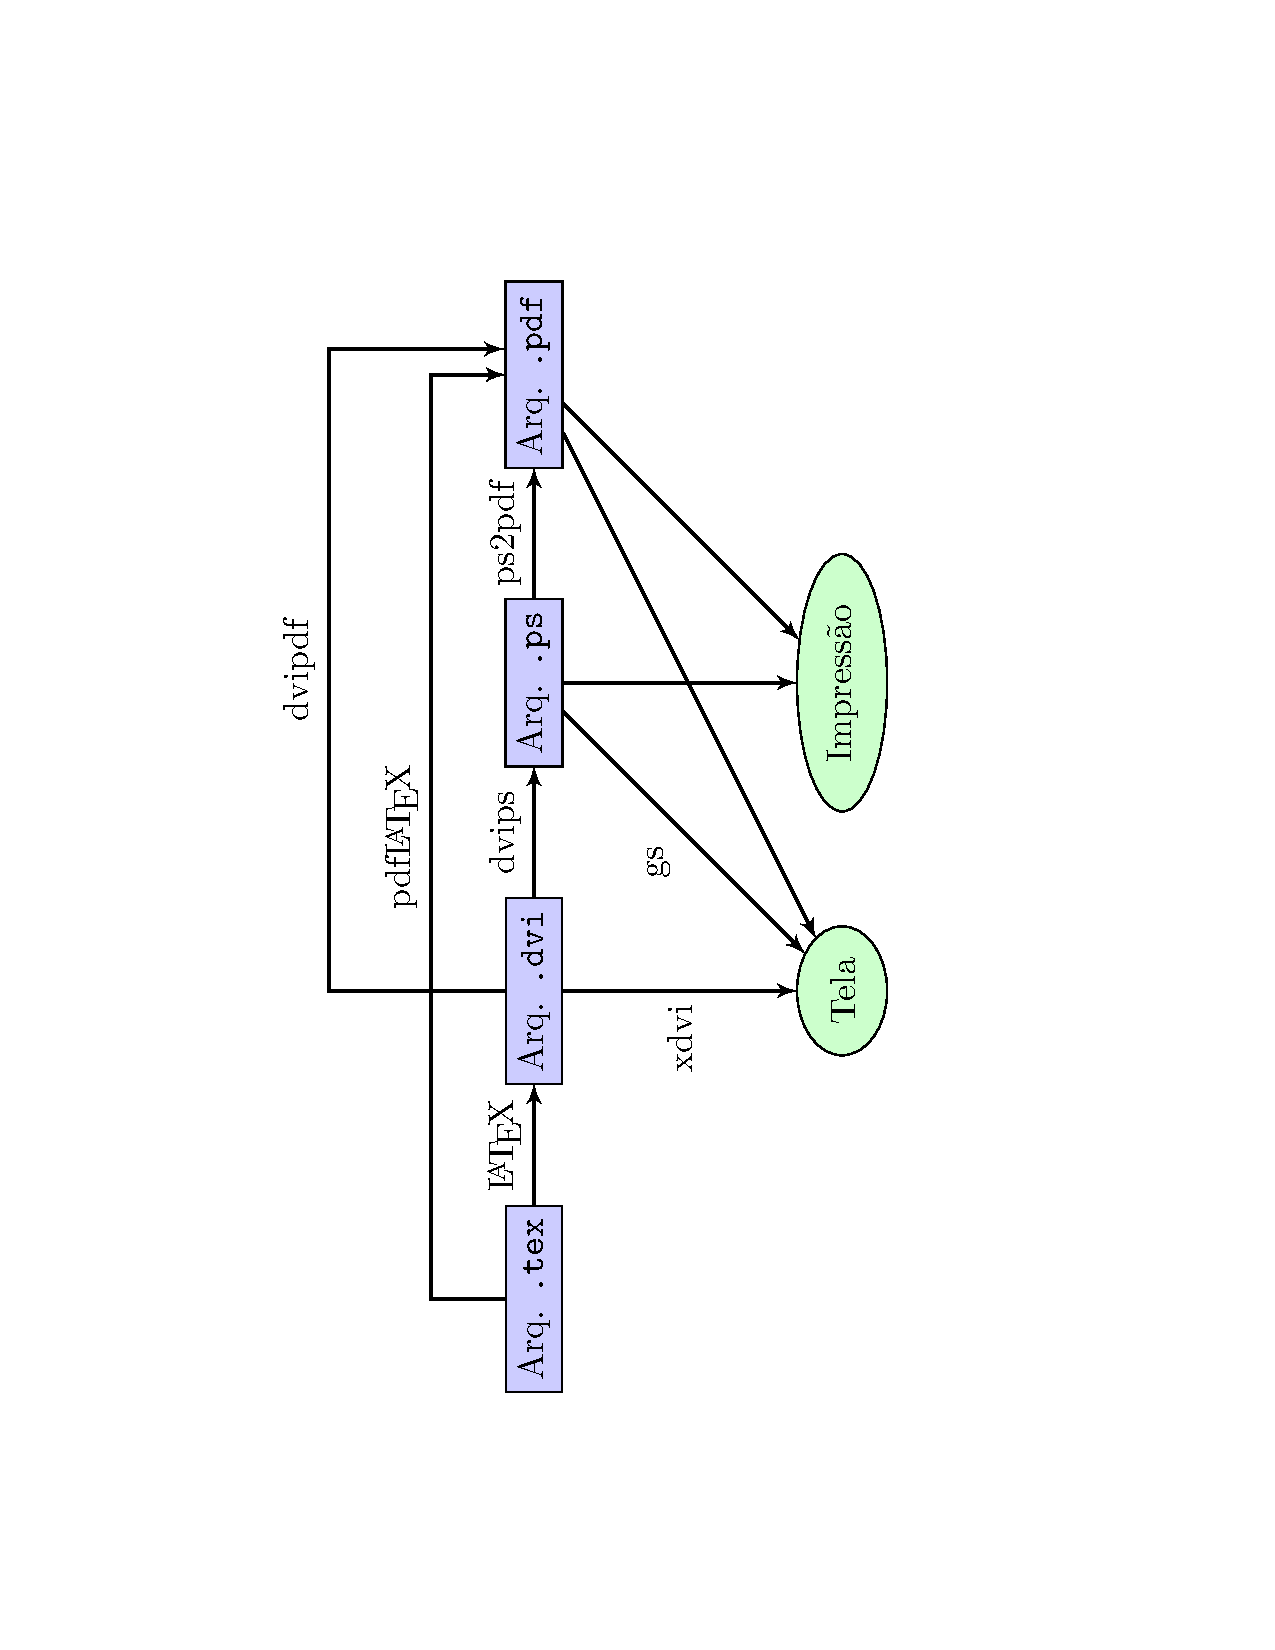
\includegraphics[scale=0.6,angle=-90,trim={4.5cm 1cm 6cm 1cm},clip]{./docs/figs/diagramacomp2.pdf}
    \end{center}
\vspace{4mm}
\legenda{Compilação de um documento \LaTeX{}.}
\label{fig:complatex}
\FONTE{Adaptado de \url{http://www.texample.net/tikz/examples/tex-workflow/}.}
\end{figure}

Na Figura \ref{fig:complatex}, observe que o compilador puro {\tt latex} da linguagem, cria um documento na extensão {\tt .dvi}. Esta extensão, \textit{Device Independent Format} (DVI), é o formato original dos documentos compilados pela linguagem e faz parte apenas do ecossistema do \TeX{}/\LaTeX{}. Por outro lado, é muito comum obter documentos no formato \textit{Portable Document Format} (PDF), o qual suporta mais cores, permite melhores níveis de compressão e é formato padrão de documento eletrônicos. Para isto, a partir do compilador {\tt latex}, pode-se utilizar algum tipo de conversor (e.g., {\tt dvi2ps}) e então, converter para o formato PDF a partir do documento \textit{PostScrpt} (PS). Nesta etapa, também pode-se utilizar outro conversor (eg., {\tt ps2pdf}) para então se obter o documento PDF final. Por outro lado, o compilador {\tt pdflatex} realiza estas etapas intermediárias de forma direta, i.e., a partir de um documento \LaTeX{} ({\tt .tex}), pode-se obter o documento PDF ({\tt .pdf}) diretamente. 

O compilador {\tt pdflatex} é o compilador mais popular. Apesar disso, ele não suporta algumas características mais modernas, como o suporte ao formato \textit{OpenType}\footnote{Um formato de fontes escalável, tal como uma imagem vetorial.}. O {\tt pdflatex} não suporta nativamente a codificação \textit{8-bit Unicode Transformation Format} (UTF-8, veja mais detalhes na Seção \ref{sec:acentos} adiante). Para amenizar estas deficiências, compiladores mais modernos foram desenvolvidos. Entre eles, pode-se citar o \XeLaTeX{} (pronuncia-se ``QueLaTec'' ou ``QuiLaTec'') e o \LuaTeX{}. Ambos suportam a codificação UTF-8 nativamente, além de permitirem a utilização de formatos de fontes mais modernas como \textit{OpenType}.

No Exemplo \ref{exe_doc}, apresenta-se um trecho de código no qual é mostrado o aspecto geral de um documento \LaTeX{}, escrito na sua forma mais simples:

\begin{texexptitled}[breakable,center lower,enhanced jigsaw,middle=2mm,listing side comment,righthand width=6cm,compilable listing,run latex,run dvips,run ps2pdf,pdf comment,comment style={raster columns=1},freeze pdf]{Um documento \LaTeX{} mínimo}{exe_doc}
\documentclass{article}
\usepackage[utf8]{inputenc}
\usepackage{lipsum}

% Este é um comentário

\title{Título}
\author{Nome}
\date{\today}

\begin{document}

\maketitle

\section{Seção}

% Este é um outro comentário

\lipsum[1]

\subsection{Subseção}

\lipsum[2]

\end{document}
\end{texexptitled}

No Exemplo \ref{exe_doc} acima, observe que um documento \LaTeX{} possui uma estrutura específica. Esta estrutura é iniciada com uma descrição do tipo de documento dado pelo comando \mintinline{latex}{documentclass} (no Exemplo \ref{exe_doc} indicando que o documento tem o formato de \textit{article}, i.e., um artigo). Tudo o que é escrito entre esta instrução e a próxima ({\tt document}), é chamada de ``preâmbulo''. Nesta seção podem ser carregados pacotes específicos da linguagem que permitem o uso de diferentes ambientes além de outros tipos de \textit{macros} (veja na Tabela \ref{tab:pacotes} do Apêndice A os pacotes utilizados neste documento). Entre as palavras reservadas \mintinline{latex}{begin} e \mintinline{latex}{end}, o documento em si é escrito. Além disso, observe também que dois comentários estão inseridos no documento, os quais não aparecem na versão compilada. Um comentário na linguagem \TeX{} ou \LaTeX{} é iniciado pelo caracter especial \%. Recomenda-se aos usuários a utilização de comentários para a organização dos seus documentos, seja para explicar \textit{macros}, separar as seções, ou mesmo remover temporariamente partes do texto. Documentos \LaTeX{}, independente da sua classe (e.g., \textit{book}, \textit{report}, \textit{article} e \textit{letter}), podem ser muito simples ou complexos. O estilo para Teses e Dissertações do INPE (apresentado no Capítulo \ref{cap:parteIV}), é um exemplo de documento complexo que inclui estilo e formatação próprios, que tornam a sua visualização bastante distinta.

Durante o aprendizado da linguagem, é bastante frequente a busca por informações na \textit{internet}. A \textit{internet} está repleta de \textit{sites} que trazem exemplos de códigos prontos que mostram como obter determinado resultado. No Exemplo \ref{exe_doc}, foi mostrado um documento mínimo e este tipo de documento serve como base para se testar pacotes diferentes, ambientes novos e outros tipos de \textit{macros}.

\begin{marker}
  Na \textit{internet} é muito comum encontrar exemplos simplificados de documentos. Ao procurar por estes exemplos em inglês, utilize as palavras-chave ``Latex \textit{Minimal Working Example}'' ou ``Latex MWE''.
\end{marker}

Pacotes no \LaTeX{} são extensões da linguagem que permitem que novos marcadores e comandos sejam utilizados. Há muitos pacotes que são populares por suas funcionalidades. Por exemplo, caso seja necessário utilizar páginas nos modos retrato e paisagem no mesmo documento, pode-se utilizar o pacote {\tt rotating}. Neste caso, deve-se incluir o comando \mintinline{latex}{\usepackage{rotating}} no preâmbulo do documento. O pacote {\tt xcolor} é utilizado quando se deseja utilizar cores diferentes no documento. Outro pacote útil, é o {\tt minted}, que permite listar códigos e destacar as palavras-chave de uma determinada linguagem, além de inserir numeração nas linhas de um código. Para a inserção de imagens vetoriais, pode-se utilizar os pacotes {\tt tickz} ou {\tt pstricks}, os quais provêm ambientes específicos para esta finalidade. Há também pacotes específicos para a confecção de tabelas, como o {\tt tabular}. Neste documento, uma série de pacotes são carregados (veja a Tabela \ref{tab:pacotes} do Apêndice A), a partir dos quais são mostrados os exemplos da linguagem \LaTeX{}. Especificamente para este propósito, utiliza-se o pacote {\tt tcolorbox}. Com este pacote, são construídas as caixas com as dicas, os exemplos e os exercícios. No estilo do INPE, apresentado em detalhes no Capítulo \ref{cap:parteIII}, muitos pacotes já são carregados por padrão, de forma que o usuário não precisa se preocupar em descobrir qual pacote precisa ser carregado quando, por exemplo, precisar inserir legendas nas figuras que inserir. Para esta finalidade, pode-se utilizar os pacotes {\tt caption} e {\tt subcaption}.

Entretanto, para quem está iniciando na utilização da linguagem \LaTeX{}, certamente encontrará dificuldades nesse entendimento. Há uma diversidade de pacotes e encontrar informações sobre eles é pode ser confuso. Orienta-se, portanto, sempre ter como referência o \textit{site} do \textit{Comprehensive TeX Archive Network} (CTAN), o qual pode ser acessado pelo endereço \url{https://www.ctan.org/}. No CTAN podem ser encontradas as referências e documentações de todos os pacotes do \LaTeX{}. Se algum pacote não estiver disponível na distribuição em uso do \LaTeX{}, pode-se baixar o arquivo referente ao pacote e adicioná-lo no local apropriado no computador. Por exemplo, durante a escrita deste documento, decidiu-se utilizar o pacote {\tt material-colors} (veja a Seção \ref{sec:pal_cores}). Este pacote não está disponível nativamente no compilador \LaTeX{} do editor \textit{online} do \textit{Overleaf}, mas foi possível obtê-lo a partir da página do projeto no CTAN (\url{https://www.ctan.org/pkg/xcolor-material}) e adicioná-lo facilmente ao projeto deste documento.

Com uma ideia mais clara sobre o aspecto de um documento \LaTeX{}, é possível utilizar o Exemplo \ref{exe_doc} para compilação. Neste exemplo, será considerado processo manual de compilação. Para começar, salve o exemplo em um arquivo texto. Pelo terminal, naveue até o diretório onde o arquivo foi salvo (neste exemplo, o arquivo foi salvo com o nome {\tt exe\_doc.tex}). Para compilar o documento do Exemplo \ref{exe_doc}, basta seguir a sequência de comandos a seguir:

\begin{meucomando}
latex exe_doc.tex 
\end{meucomando}

Com o comando {\tt latex} acima, serão gerados os seguintes arquivos, sendo o principal deles, o arquivo {\tt exe\_doc.dvi}:

\begin{itemize}
  \item {\tt exe\_doc.tex}  
  \item {\tt exe\_doc.log}
  \item {\tt exe\_doc.dvi}
  \item {\tt exe\_doc.aux}
\end{itemize}

Em seguida, executar o programa {\tt dvips}:

\begin{meucomando}
dvips exe_doc
\end{meucomando}

Com o comando {\tt dvips} acima, será gerado o arquivo {\tt exe\_doc.ps}. Por fim, basta utilizar o comando {\tt ps2pdf} para gerar o arquivo {\tt exe\_doc.pdf}:

\begin{meucomando}
ps2pdf exe_doc
\end{meucomando}

Assim como é moistrado no diagrama da Figura \ref{fig:complatex}, é possível utilizar o comando {\tt pdflatex} para gerar o arquivo final {\tt exe\_doc.pdf} em uma única etapa, a partir do arquivo original {\tt exe\_doc.tex}. Utilizando a linha de comando para a compilação manual de documentos \LaTeX{}, é possível também emular o mesmo comportamente de alguns editores WYSIWYG. No Apêndice B, são apresentadas algumas opções possíveis com o comando {\tt latexmk}.

Se o leitor estiver utilizando algum editor WYSIWYG, certamente achará mais fácil pressionar o botão ``compile'' ou ``build and view'' (como no caso do editor \TeX \textit{Studio}). Independente da forma como o documento é compilado, os resultados serão os mesmos.

Nas próximas seções, serão introduzidos os diversos marcadores e comandos que podem ser utilizados para alterar a aparência e o posicionamento dos textos e parágrafos, figuras, tabelas e demais elementos que constituem um documento formatado no \LaTeX{}.

\subsection{Caracteres e símbolos especiais}
\label{sec:carac_especiais}

No \LaTeX{} há 10 tipos de caracteres especiais. São eles:

\begingroup
\renewcommand{\labelenumi}{\arabic{enumi})}
\begin{multicols}{5}
    \begin{enumerate}
        \item \textbackslash
        \item \#
        \item \$
        \item \%
        \item \&
        \item \^{}
        \item \_
        \item \{
        \item \}
        \item \texttt{\~{}}
    \end{enumerate}
\end{multicols}
\endgroup

Às vezes é necessários utilizá-los ao longo do texto. Por exemplo, o \% (porcento) é utilizado para inserir comentários no corpo do texto (veja o Exemplo \ref{exe_doc}). O uso destes caracteres ao longo do texto requer alguns cuidados especiais, e então, faz-se necessário destacá-los. Há duas formas de fazer isso. 1) escapando-os ou 2) utilizando comandos especiais para a sua correta representação.

Na primeira forma, basta utilizar a {\tt $\backslash$} (barra invertida). Na segunda, utilizam-se comandos específicos do \LaTeX{}. Veja o Exemplo \ref{exe_caracesp} a seguir:

\begin{texexptitled}[breakable,center lower,enhanced,middle=2mm,listing side text]{Marcação para caracteres especiais}{exe_caracesp}
\textbackslash
\\
\^{}
\\
\texttt{\~{}}
\end{texexptitled}

Outro caractere especial, são as `' (aspas). No \LaTeX{}, aspas simples são marcadas como \mintinline{latex}{`'}, enquanto que aspas duplas são marcadas como \mintinline{latex}{``''}. Portanto, palavras e expressões grafadas entre aspas simples ou duplas, devem aparecer como `aspas simples' e ``aspas duplas'', ao invés de 'aspas simples' ou "aspas duplas"  (como acontece quando se utiliza o acento trema "  do teclado).

\begin{marker}
  No Exemplo \ref{exe_caracesp}, o comando \mintinline{latex}{\\} pula uma linha. Para esta finalidade, pode-se utilizar também o comando \mintinline{latex}{\newline}, ou simplesmente uma linha e branco.
\end{marker}

No Exemplo \ref{exe_caracesp}, observe que a barra invertida é produzida pelo comando \mintinline{latex}{\textbackslash} ou pelo comando \mintinline{latex}{$\backslash$}, quando em modo matemático (veja mais detalhes sobre o modo matemático na Seção \ref{sec:mat_eqs}).

\subsection{Acentos}
\label{sec:acentos}

No \LaTeX{}, os acentos podem ser escritos de forma literal, i.e., acentuando-se diretamente as vogais sem a necessidade de marcadores especiais, desde que os pacotes necessários estejam carregados. O {\tt inputenc} é um pacote do \LaTeX{} que fornece os formatos de marcação e linguagem adequados para a acentuação de, por exemplo, caracteres latinos acentuados. Além disso, para que as estruturas do texto que fazem referências à figuras e tabelas fiquem corretamente grafadas no idioma da escrita, é necessário utilizar-se o pacote {\tt babel} indicando o dialeto no qual se está escrevendo. Outro pacote importante é o {\tt fontenc} que trata da apresentação correta dos caracteres especiais, i.e., aqueles que são acentuados.

Para digitar acentos de forma natural, é necessário carregar os pacotes a seguir, no preâmbulo do documento:

\begin{itemize}
    \item \mintinline{latex}{\usepackage[brazilian]{babel}}
    \item \mintinline{latex}{\usepackage[T1]{fontenc}}
    \item \mintinline{latex}{\usepackage[utf8]{inputenc}}\footnotemark[1]
\end{itemize}

\footnotetext[1]{Pode-se utilizar também o pacote {\tt latin1}, com o comando \mintinline{latex}{\usepackage[latin1]{inputenc}}. Ambos os pacotes, {\tt utf-8} e {\tt latin1} fornecem o suporte ao UNICODE. Se o usuário quiser utilizar o formato \textit{OpenType}, evite utilizar estes pacotes e utilize compiladores mais modernos como o \XeLaTeX{} ou o \LuaTeX{}.}

\begin{marker}
  No estilo do INPE, os pacotes relacionados acima são pré-carregados. Porém, se o usuário utilizar os compiladores \XeLaTeX{} ou \LuaTeX{}, o usuário encontrará erros enquanto o pacote {\tt inputenc} estiver carregado. Veja mais informações na Seção \ref{sec:oriesp} do Capítulo \ref{cap:parteIII}.
\end{marker}

Entretanto, em algumas situações é necessário marcar os acentos de forma explícita (e.g., na edição de um arquivo de referências do Bib\TeX{}, cujo formato é apresentado na Seção \ref{sec:refs}).

No Exemplo \ref{exe_acentos} a seguir, são mostrados os acentos mais comuns.

\begin{texexptitled}[breakable,center lower,enhanced,middle=2mm,listing side text]{Uso de acentos latinos no \LaTeX{}}{exe_acentos}
\'A \'E \'I \'O \'U

\'a \'e \'i \'o \'u

\^a \^A \~a \~A \`a \`A \~o \~O

\^e \^E \^o \^O

\"u \"U

\c{c} \c{C}
\end{texexptitled}

\begin{marker}
  Outras marcações especiais para acentuação de caracteres podem ser encontradas em \url{https://en.wikibooks.org/wiki/LaTeX/Special_Characters}.
\end{marker}

\subsection{Tipos, tamanhos e estilos de letras}
\label{sec:marc_text}

O texto básico pode ser marcado em estilos comuns, como o \textit{itálico}, o \underline{sublinhado}, o \textbf{negrito}, o texto \textsuperscript{sobrescrito} e o texto \textsubscript{subscrito}. Veja no Exemplo \ref{exe_estilos} a seguir:

\begin{texexptitled}[breakable,center lower,enhanced,middle=2mm,listing side text]{Marcações mais mais comuns em fontes}{exe_estilos}
\textit{itálico}       \\
\textsl{inclinado}     \\
\underline{sublinhado} \\
\textbf{negrito}       \\
\textsuperscript{o}C   \\
H\textsubscript{2}O
\end{texexptitled}

No Exemplo \ref{exe_estilos}, observe as diferenças entre o texto itálico produzido com o marcador \mintinline{latex}{\textit} e o texto inclinado produzido pelo marcador \mintinline{latex}{\textsl}. No primeiro caso, as fontes produzidas são naturais, ou seja, há uma variação em itálico do tipo de fonte em uso. No segundo caso, a fonte em uso é renderizada a partir da inclinação da fonte natural. 

\begin{marker}
Dependendo do tipo de fonte utilizado, as diferenças entre os tipos itálico e inclinado podem ser mais evidentes. Veja mais no Exemplo \ref{exe_font}.
\end{marker}

Outros estilos também podem ser utilizados, mas podem depender de outros pacotes. Dois pacotes que fornecem estilos de marcações sobre as palavras, são o \mintinline{latex}{ulem} e o \mintinline{latex}{cancel}. Para utilizá-los, deve-se antes carregar os pacotes necessários com os comandos \mintinline{latex}{\usepackage{ulem}} e \mintinline{latex}{\usepackage{cancel}}, os quais devem ser inseridos no preâmbulo do documento. 

Com o pacote \mintinline{latex}{ulem}, pode-se riscar as palavras (forma mais comum). Veja no Exemplo \ref{exe_ulem}:

\begin{texexptitled}[breakable,center lower,enhanced,middle=2mm,listing side text]{Marcação em texto com o pacote \mintinline{latex}{ulem}}{exe_ulem}
\sout{palavra riscada}
\end{texexptitled}

Diferente do que se obtém com o pacote {\tt ulem}, com o pacote {\tt cancel} pode-se riscar expressões matemáticas. Veja o Exemplo \ref{exe_cancel} a seguir (mais exemplos de expressões matemáticas e ambientes específicos são apresentados na Seção \ref{sec:mat_eqs}):

\begin{texexptitled}[breakable,center lower,enhanced,middle=2mm,]{Marcação em expressões matemáticas com o pacote \mintinline{latex}{cancel}}{exe_cancel}
$$\frac{x^{2} - 5x}{x^{2}} = \frac{\cancel{x} \cdot (x - 5)}{x^{\cancel{2}}}$$

$$\frac{x^{2} - 5x}{x^{2}} = \frac{\bcancel{x} \cdot (x - 5)}{x^{\bcancel{2}}}$$

$$\lim_{x \to 1}{\frac{\cancel{(x - 1)} \cdot (x + 1)}{\cancel{(x - 1)}}} = \lim_{x \to 1}{(x + 1)}$$

$$\frac{\cancelto{5}15}{{\cancel{3}}} = 5$$

$$\xcancel{\frac{x^{2} - 5x + 10}{\sqrt{81}}}$$
\end{texexptitled}

No \LaTeX{}, ao longo de um parágrafo, é possível alterar o tamanho da fonte. O padrão do \LaTeX{} compreende 10 tamanhos diferentes, os quais são mostrados no Exemplo \ref{exe_tamfonte}.

\begin{texexptitled}[breakable,center lower,enhanced,middle=2mm,listing side text]{Tamanhos de fontes}{exe_tamfonte}
{\Huge Huge}                 \\
{\huge huge}                 \\
{\LARGE LARGE}               \\
{\Large Large}               \\
{\large large}               \\
{\normalsize normalsize}     \\
{\small small}               \\
{\footnotesize footnotesize} \\
{\scriptsize scriptsize}     \\
{\tiny tiny}
\end{texexptitled}

Para alterar o tamanho de uma fonte localmente, basta utilizar os marcadores do Exemplo \ref{exe_tamfonte} como \mintinline{latex}{{\large palavra}}. Veja no Exemplo \ref{exe_tamfontefrase} como misturar diferentes tamanhos de fonte em uma mesma frase:

\begin{texexptitled}[breakable,center lower,enhanced,middle=2mm]{Texto com diferentes tamanhos de fontes}{exe_tamfontefrase}
À noite, vovô {\large Kowalsky} vê o {\huge ímã} cair no pé do pinguim {\Huge queixoso} e vovó põe açúcar no {\footnotesize chá} de {\tiny tâmaras} do jabuti feliz. 
\end{texexptitled}

No \LaTeX{} é possível também alterar o tipo da fonte. Alguns estilos incluem fontes no estilo \texttt{máquina de escrever}, \textsf{sem serifa} e \textrm{com serifa}. No Exemplo \ref{exe_font} é mostrado como alterar o estilo das fontes.

\begin{texexptitled}[breakable,center lower,enhanced,middle=2mm]{Estilos de fontes}{exe_font}
\texttt{Máquina de Escrever} | \texttt{\textit{Máquina de Escrever, em itálico}} | \texttt{\textsl{Máquina de Escrever, inclinado}}

\textsf{Sem Serifa} | \textsf{\textit{Sem Serifa, em itálico}} | \textsf{\textsl{Sem Serifa, inclinado}}

\textrm{Com Serifa, estilo Romano} | \textrm{\textit{Com Serifa, estilo Romano itálico}} | \textrm{\textsl{Com Serifa, estilo Romano inclinado}}
\end{texexptitled}

\subsection{Títulos e seções}
\label{sec:tit_secs}

No \LaTeX{}, é possível organizar o texto utilizando seções em até 7 níveis, os quais estão sumarizados na Tabela \ref{tab:tit_secs} a seguir.

% Dica dos expaçamentos: https://tex.stackexchange.com/questions/10535/how-to-force-a-table-into-page-width/56552
\begin{table}[H]
\caption{Títulos e Seções de um documento \LaTeX{}.}
\begin{center}
  \begin{tabular}{p{5cm}p{5cm}c}
    \toprule
    \textbf{Seção} & \textbf{Comando}                & \textbf{Nível} \\
  	\midrule
    Parte          & \mintinline{latex}{\part}       & -1             \\
    Capítulo       & \mintinline{latex}{\chapter}    & 0              \\
    Seção          & \mintinline{latex}{\section}    & 1              \\
    Subseção       & \mintinline{latex}{\subsection} & 2              \\
    Parágrafo      & \mintinline{latex}{\par}        & 3              \\
    Subparágrafo   & \mintinline{latex}{\subpar}     & 4              \\
    \bottomrule
  \end{tabular}
\end{center}
\label{tab:tit_secs}
\FONTE{Adaptado de \url{https://www.overleaf.com/learn/latex/Sections_and_chapters}.}
\end{table}

Na Seção \ref{sec:intro_latex} foram mostradas as classes mais comuns disponíveis para documentos \LaTeX{}. Observe que as partes de conteúdo marcadas como \mintinline{latex}{part} e \mintinline{latex}{chapter} estão disponíveis apenas para as classes \mintinline{latex}{report} e \mintinline{latex}{book}. Uma das vantagens da edição de documento na linguagem \LaTeX{} é que a numeração de partes, figuras, tabelas, equações etc é automática. Isto significa que sempre que se iniciar um novo capítulo ou seção, a numeração é automaticamente incrementada. Se o texto for reorganizado, de forma que uma seção ou capítulo é transferido para outra posição no texto, eles são automaticamente renumerados, respeitando a ordem em que são apresentados. Entretanto, é possível omitir a numeração destes elementos textuais através da inserção de um * (asterisco). Veja o efeito disto no Exemplo \ref{exe_secsnum} a seguir.

\begin{texexptitled}[breakable,center lower,enhanced jigsaw,middle=2mm,listing side comment,righthand width=6cm,compilable listing,run latex,run dvips,run ps2pdf,pdf comment,comment style={raster columns=1},freeze pdf]{Numeração automática dos elementos textuais}{exe_secsnum}
\documentclass[17pt]{extarticle}
\usepackage[utf8]{inputenc}
\usepackage{lipsum}
\usepackage{extsizes}

\title{Título}
\author{Nome}
\date{\today}

\begin{document}

\maketitle

\tableofcontents

\section{Uma Seção}

\lipsum[1]

\subsection*{Uma subseção}

\lipsum[2]

\end{document}
\end{texexptitled}

No Exemplo \ref{exe_secsnum} observe que o sumário foi inserido no corpo do texto utilizando-se o comando \mintinline{latex}{\tableofcontents}. Este comando é responsável por adicionar os capítulos, seções, subseções e outras partes do texto ao sumário. Observe também que a subseção marcada por \mintinline{latex}{\subsection*{Uma subseção}} não foi adicionada ao sumário porque ela foi marcada com \mintinline{latex}{\subsection*} ou invés de \mintinline{latex}{\subsection}. O asterisco pode ser utilizado com a mesma finalidade em outros ambientes, como figuras, tabelas e equações. Além disso, note que o comando \mintinline{latex}{\maketitle} é responsável por posicionar o título, o nome do autor e a data no início do documento. Dependendo da classe de documentos utilizada, o aspecto e a posição do título e do sumário (e de outras listas que se fizerem necessárias) poderão ser diferentes.

\begin{marker}
O pacote {\tt extsizes} foi utilizado no Exemplo \ref{exe_secsnum} com o objetivo de se aumentar globalmente o tamanho da fonte no documento do exemplo. Observe que com o uso deste pacote o nome da classe do documento é {\tt extarticle} ao invés de {\tt article}, como no caso do Exemplo \ref{exe_doc}. Veja mais sobre o pacote {\tt extsize} no endereço \url{https://ctan.org/pkg/extsizes}.
\end{marker}

\subsection{Cores e Paletas de Cores}
\label{sec:pal_cores}

% REF: https://martin-thoma.com/colors-in-latex/
%A paleta de cores padrão do LaTeX pode ser alterada.
Em um documento \LaTeX{}, é possível utilizar cores predefinidas ou definir cores seguindo um determinado padrão. As cores padrão que geralmente são utilizadas em um documento \LaTeX{}, i.e., aquelas que não dependem de pacotes extras, são apresentadas a seguir, com os nomes das cores anotadas abaixo das suas respectivas caixas.

\begin{center}
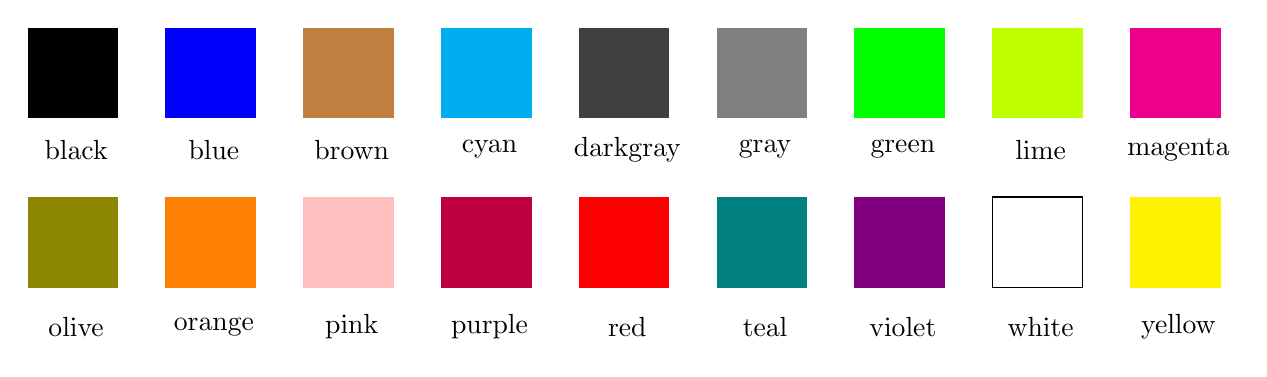
\begin{tikzpicture}
\fill [black] (0,0) rectangle ++(1.15,1.15);
\draw (0.615,-0.4) node {black};
\fill [blue] (1.75,0) rectangle ++(1.15,1.15);
\draw (2.365,-0.4) node {blue};
\fill [brown] (3.5,0) rectangle ++(1.15,1.15);
\draw (4.115,-0.4) node {brown};
\fill [cyan] (5.25,0) rectangle ++(1.15,1.15);
\draw (5.865,-0.4) node {cyan};
\fill [darkgray] (7,0) rectangle ++(1.15,1.15);
\draw (7.615,-0.4) node {darkgray};
\fill [gray] (8.75,0) rectangle ++(1.15,1.15);
\draw (9.365,-0.4) node {gray};
\fill [green] (10.5,0) rectangle ++(1.15,1.15);
\draw (11.115,-0.4) node {green};
\fill [lime] (12.25,0) rectangle ++(1.15,1.15);
\draw (12.865,-0.4) node {lime};
\fill [magenta] (14,0) rectangle ++(1.15,1.15);
\draw (14.615,-0.4) node {magenta};

\fill [olive] (0,-1) rectangle ++(1.15,-1.15);
\draw (0.615,-2.65) node {olive};
\fill [orange] (1.75,-1) rectangle ++(1.15,-1.15);
\draw (2.365,-2.65) node {orange};
\fill [pink] (3.5,-1) rectangle ++(1.15,-1.15);
\draw (4.115,-2.65) node {pink};
\fill [purple] (5.25,-1) rectangle ++(1.15,-1.15);
\draw (5.865,-2.65) node {purple};
\fill [red] (7,-1) rectangle ++(1.15,-1.15);
\draw (7.615,-2.65) node {red};
\fill [teal] (8.75,-1) rectangle ++(1.15,-1.15);
\draw (9.365,-2.65) node {teal};
\fill [violet] (10.5,-1) rectangle ++(1.15,-1.15);
\draw (11.115,-2.65) node {violet};
\draw[fill=white] (12.25,-1) rectangle ++(1.15,-1.15);
\draw (12.865,-2.65) node {white};
\fill [yellow] (14,-1) rectangle ++(1.15,-1.15);
\draw (14.615,-2.65) node {yellow};
\end{tikzpicture}
\end{center}

Cores podem ser utilizadas de formas diferentes em um documento \LaTeX{}. Mas assim como em qualquer editor de textos WYSIWYG, as cores do texto podem ser aplicadas em palavras individuais, frases ou parágrafos. Veja o Exemplo \ref{exe_cor1} a seguir.

\begin{texexptitled}[breakable,center lower,enhanced,middle=2mm]{Texto com fonte colorida, paleta padrão}{exe_cor1}
\textit{\color{pink}{Quem} \color{cyan}{traz} \color{green}{CD}, \color{olive}{LP}, \color{violet}{fax}, \color{blue}{engov} \color{red}{e} \color{lime}{whisky} \color{orange}{JB?}}
\end{texexptitled}

Além de modificar a cor das fontes, é possível também marcá-las de forma que o fundo fique colorido, como mostrado no Exemplo \ref{exe_cor3}.

\begin{texexptitled}[breakable,center lower,enhanced,middle=2mm]{Texto com fundo colorido, paleta padrão}{exe_cor3}
\textit{\colorbox{pink}{Quem} \colorbox{cyan}{traz} \colorbox{green}{CD}, \colorbox{olive}{LP}, \colorbox{violet}{\color{white}{fax}}, \colorbox{blue}{\color{white}{engov}} \colorbox{red}{e} \colorbox{lime}{whisky} \colorbox{orange}{JB?}}
\end{texexptitled}

É possível também escolher uma paleta de cores diferente, e.g., a patela de cores do projeto \href{https://ethanschoonover.com/solarized/}{\textit{Solarized}}. Para utilizá-la, basta carregar o pacote \mintinline{latex}{\usepackage{solarized}} no preâmbulo do documento e aplicar as cores conforme o Exemplo \ref{exe_corsol} adiante. A paleta de cores do ``Solarized'' possui as seguintes cores básicas:

\begin{center}
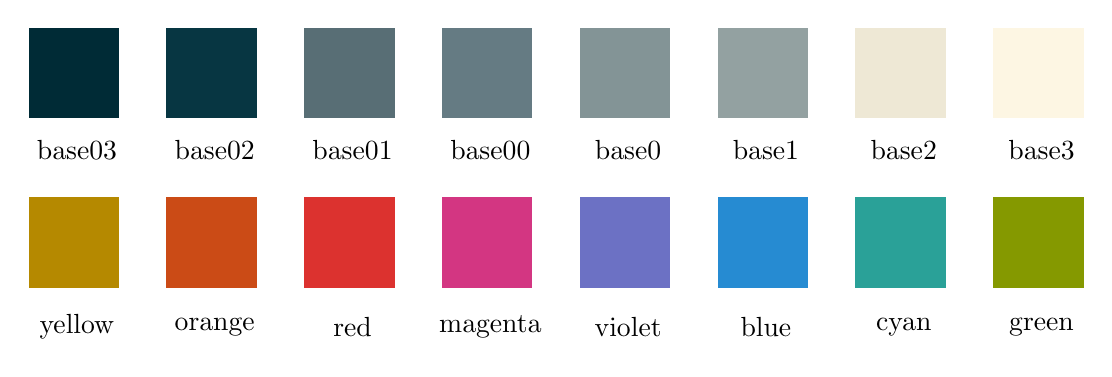
\begin{tikzpicture}
\fill [solarized-base03] (0,0) rectangle ++(1.15,1.15);
\draw (0.615,-0.4) node {base03};
\fill [solarized-base02] (1.75,0) rectangle ++(1.15,1.15);
\draw (2.365,-0.4) node {base02};
\fill [solarized-base01] (3.5,0) rectangle ++(1.15,1.15);
\draw (4.115,-0.4) node {base01};
\fill [solarized-base00] (5.25,0) rectangle ++(1.15,1.15);
\draw (5.865,-0.4) node {base00};
\fill [solarized-base0] (7,0) rectangle ++(1.15,1.15);
\draw (7.615,-0.4) node {base0};
\fill [solarized-base1] (8.75,0) rectangle ++(1.15,1.15);
\draw (9.365,-0.4) node {base1};
\fill [solarized-base2] (10.5,0) rectangle ++(1.15,1.15);
\draw (11.115,-0.4) node {base2};
\fill [solarized-base3] (12.25,0) rectangle ++(1.15,1.15);
\draw (12.865,-0.4) node {base3};

\fill [solarized-yellow] (0,-1) rectangle ++(1.15,-1.15);
\draw (0.615,-2.65) node {yellow};
\fill [solarized-orange] (1.75,-1) rectangle ++(1.15,-1.15);
\draw (2.365,-2.65) node {orange};
\fill [solarized-red] (3.5,-1) rectangle ++(1.15,-1.15);
\draw (4.115,-2.65) node {red};
\fill [solarized-magenta] (5.25,-1) rectangle ++(1.15,-1.15);
\draw (5.865,-2.65) node {magenta};
\fill [solarized-violet] (7,-1) rectangle ++(1.15,-1.15);
\draw (7.615,-2.65) node {violet};
\fill [solarized-blue] (8.75,-1) rectangle ++(1.15,-1.15);
\draw (9.365,-2.65) node {blue};
\fill [solarized-cyan] (10.5,-1) rectangle ++(1.15,-1.15);
\draw (11.115,-2.65) node {cyan};
\fill [solarized-green] (12.25,-1) rectangle ++(1.15,-1.15);
\draw (12.865,-2.65) node {green};
\end{tikzpicture}
\end{center}

Para utilizar as novas cores, basta utilizar um dos nomes definidos pela paleta, precedido por \mintinline{latex}{solarized-nome-da-cor}. Veja o Exemplo \ref{exe_corsol} a seguir.

\begin{texexptitled}[breakable,center lower,enhanced,middle=2mm]{Texto com fundo colorido, paleta \textit{Solarized}}{exe_corsol}
\textit{\colorbox{solarized-magenta}{Quem} \colorbox{solarized-cyan}{traz} \colorbox{solarized-green}{CD}, \colorbox{solarized-red}{LP}, \colorbox{solarized-violet}{\color{solarized-base3}{fax}}, \colorbox{solarized-base1}{\color{solarized-base2}{engov}} \colorbox{solarized-red}{e} \colorbox{solarized-yellow}{whisky} \colorbox{solarized-orange}{JB?}}
\end{texexptitled}

\begin{marker}
Mais informações sobre o pacote {\tt xcolor-solarized} podem ser encontradas em \url{https://www.ctan.org/pkg/xcolor-solarized}.
\end{marker}

Outra paleta de cores harmoniosa, é provida pelo pacote {\tt xcolor-material}. Esta é a paleta de cores do \href{https://material.io/}{\textit{Material Design} do Google}. Para utilizá-la, basta carregar o pacote \mintinline{latex}{\usepackage{xcolor-material}} no preâmbulo do documento. 

As cores básicas do pacote {\tt xcolor-material} são as seguintes (além do branco e preto):

\begin{center}
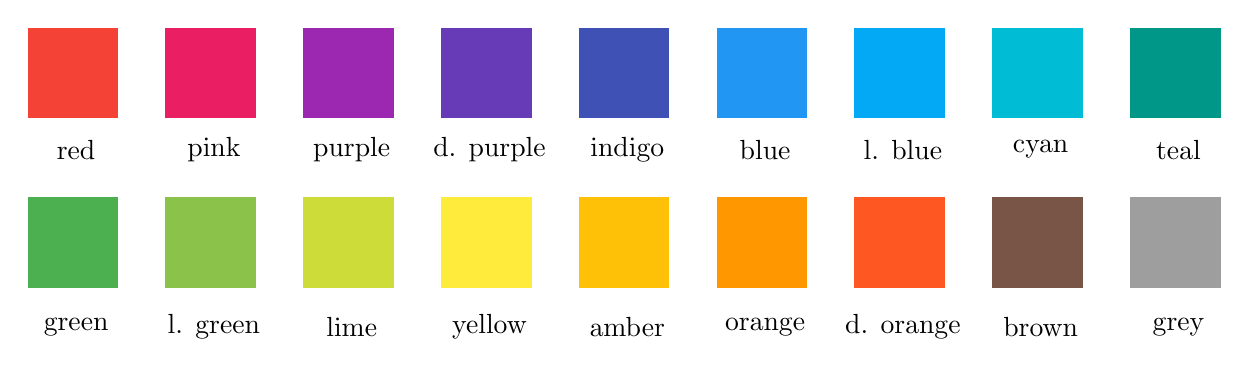
\begin{tikzpicture}
\fill [MaterialRed] (0,0) rectangle ++(1.15,1.15);
\draw (0.615,-0.4) node {red};
\fill [MaterialPink] (1.75,0) rectangle ++(1.15,1.15);
\draw (2.365,-0.4) node {pink};
\fill [MaterialPurple] (3.5,0) rectangle ++(1.15,1.15);
\draw (4.115,-0.4) node {purple};
\fill [MaterialDeepPurple] (5.25,0) rectangle ++(1.15,1.15);
\draw (5.865,-0.4) node {d. purple};
\fill [MaterialIndigo] (7,0) rectangle ++(1.15,1.15);
\draw (7.615,-0.4) node {indigo};
\fill [MaterialBlue] (8.75,0) rectangle ++(1.15,1.15);
\draw (9.365,-0.4) node {blue};
\fill [MaterialLightBlue] (10.5,0) rectangle ++(1.15,1.15);
\draw (11.115,-0.4) node {l. blue};
\fill [MaterialCyan] (12.25,0) rectangle ++(1.15,1.15);
\draw (12.865,-0.4) node {cyan};
\fill [MaterialTeal] (14,0) rectangle ++(1.15,1.15);
\draw (14.615,-0.4) node {teal};

\fill [MaterialGreen] (0,-1) rectangle ++(1.15,-1.15);
\draw (0.615,-2.65) node {green};
\fill [MaterialLightGreen] (1.75,-1) rectangle ++(1.15,-1.15);
\draw (2.365,-2.65) node {l. green};
\fill [MaterialLime] (3.5,-1) rectangle ++(1.15,-1.15);
\draw (4.115,-2.65) node {lime};
\fill [MaterialYellow] (5.25,-1) rectangle ++(1.15,-1.15);
\draw (5.865,-2.65) node {yellow};
\fill [MaterialAmber] (7,-1) rectangle ++(1.15,-1.15);
\draw (7.615,-2.65) node {amber};
\fill [MaterialOrange] (8.75,-1) rectangle ++(1.15,-1.15);
\draw (9.365,-2.65) node {orange};
\fill [MaterialDeepOrange] (10.5,-1) rectangle ++(1.15,-1.15);
\draw (11.115,-2.65) node {d. orange};
\fill [MaterialBrown] (12.25,-1) rectangle ++(1.15,-1.15);
\draw (12.865,-2.65) node {brown};
\fill [MaterialGrey] (14,-1) rectangle ++(1.15,-1.15);
\draw (14.615,-2.65) node {grey};
\end{tikzpicture}
\end{center}

Na paleta de cores mostrada acima, ``d.'' foi utilizado para abreviar a palavra \textit{deep} (como em \textit{deep purple}) e ``l.'' foi utilizada para abreviar a palavra \textit{light} (como em \textit{light green}). Para utilizar as cores do pacote {\tt xcolor-material}, deve-se referenciar as cores da seguinte forma: a cor \textit{Deep Purple} deve ser referenciada como ``MaterialDeepPurple'', ou seja, a palavra reservada ``Material'' deve preceder o nome da cor, que por sua vez, deve ser indicada com a primeira letra em caixa alta. Veja no Exemplo \ref{exe_cormaterial} como utilizar as cores deste pacote.

\begin{texexptitled}[breakable,center lower,enhanced,middle=2mm]{Texto com fundo colorido, paleta \textit{Material Design}}{exe_cormaterial}
\textit{\colorbox{MaterialRed}{Quem} \colorbox{MaterialPink}{traz} \colorbox{MaterialPurple}{CD}, \colorbox{MaterialDeepPurple}{LP}, \colorbox{MaterialIndigo}{\color{white}{fax}}, \colorbox{MaterialLightBlue}{\color{white}{engov}} \colorbox{MaterialTeal}{e} \colorbox{MaterialGreen}{whisky} \colorbox{MaterialLightGreen}{JB?}}
\end{texexptitled}

\begin{marker}
Pode ser necessário incluir o arquivo {\tt xcolor-material.sty} à sua distribuição \LaTeX{}. Veja a página do pacote para mais informações (\url{https://www.ctan.org/pkg/xcolor-material}).
\end{marker}

Além da utilização de paletas de cores pré-definidas, é possível também definir qualquer cor utilizando códigos \textit{Hypertext Markup Language} (HTML), \textit{Red Green Blue} (RGB) ou \textit{Cyan Magenta Yellow Black} (CMYK) utilizando o comando \mintinline{latex}{\definecolor}. Veja no Exemplo \ref{exe_cor4} como definir cores personalizadas.

\begin{texexptitled}[breakable,center lower,enhanced,middle=2mm]{Definindo cores personalizadas}{exe_cor4}
\definecolor{meuazul1}{HTML}{0066ff}
\definecolor{meuazul2}{rgb}{0.2,0.6,1}
\definecolor{meuazul3}{RGB}{0,204,255}
\definecolor{meuazul4}{cmyk}{0.6,0,0,0}

\begin{tikzpicture}
\fill [meuazul1] (0,0) rectangle ++(1.25,1.25);
\draw (0.6,-0.5) node {meuazul1};
\fill [meuazul2] (3,0) rectangle ++(1.25,1.25);
\draw (3.6,-0.5) node {meuazul2};
\fill [meuazul3] (6,0) rectangle ++(1.25,1.25);
\draw (6.6,-0.5) node {meuazul3};
\fill [meuazul4] (9,0) rectangle ++(1.25,1.25);
\draw (9.6,-0.5) node {meuazul4};
\end{tikzpicture}
\end{texexptitled}

\begin{marker}
Veja outras opções de paletas e cores personalizadas em \href{http://latexcolor.com}{LaTeXColor}.
\end{marker}

\subsection{Medidas}
\label{sec:medidas}

As medidas na linguagem \LaTeX{} podem ser apresentadas em unidades diversas. É comum misturá-las e isso pode ocorrer quando se reutiliza algum código encontrado na \textit{internet}, o que é bastante comum. A Tabela \ref{tab:medidas} a seguir, mostra as unidades de medida mais comuns da linguagem. Ressalta-se, entretanto, que a unidade padrão é o $\cdot$ (ponto) e que o comprimento padrão é, portanto, 1 {\tt pt}:

\begin{table}[H]
\centering
\caption{Unidades de Medidas mais Comuns no \LaTeX{}.}
\label{tab:medidas}
  \begin{tabular}{p{3cm}cc}
    \toprule
    \textbf{Unidade} & \textbf{Abreviação} & \textbf{Valor em Pontos}  \\
    \midrule
    Ponto           & {\tt pt} & 1 {\tt pt}                            \\
    Milímetro       & {\tt mm} & 1 {\tt mm} = 2,84 {\tt pts}           \\
    Centímetro      & {\tt cm} & 1 {\tt cm} = 28,4 {\tt pts}           \\
    Polegada        & {\tt in} & 1 {\tt in} = 72,27 {\tt pts}          \\
    Paica           & {\tt pc} & 1 {\tt pc} = 12 {\tt pts}             \\
    Altura de ``x'' & {\tt ex} & \textit{Depende da fonte utilizada}   \\
    Altura de ``M'' & {\tt em} & \textit{Depende da fonte utilizada}   \\
    \bottomrule
  \end{tabular}
\FONTE{Produção do autor.}
\end{table}

As unidades de medidas apresentadas na Tabela \ref{tab:medidas} mostram os valores da unidade em termos de pontos. O \LaTeX{} utiliza o ponto como referência absoluta e a escolha por uma unidade ou outra irá depender do que se quer medir ou das medidas que se quer estabelecer. As dimensões de uma página devem ser estabelecidas em unidades fixas, e.g., a folha A4 mede 210 mm (largura) por 297 mm (altura). Por outro lado, pode ser mais adequado utilizar medidas relativas, e.g., a largura de uma figura como sendo a metade da largura de uma página A4. Dessa forma, é mais fácil definir o tamanho destes elementos.

\begin{marker}
O pacote {\tt lengthconvert} pode ser útil na definição e converção de unidades de medidas no \LaTeX{}. Veja a página do pacote em \url{https://ctan.org/pkg/lengthconvert} para mais informações.
\end{marker}

Em documentos escritos na linguagem \LaTeX{}, é possível especificar as medidas relativas utilizando os valores nas unidades indicadas pela Tabela \ref{tab:medidas} e também utilizando \textit{macros} específicas para esta finalidade. Algumas destas \textit{macros} de medidas são apresentadas na Tabela \ref{tab:meds_padrao} abaixo.

\begin{table}[H]
	\centering
	\caption{Algumas Macros de Medidas do \LaTeX{}.}
	\label{tab:meds_padrao}
	\begin{tabular}{p{4cm}p{9cm}}
		\toprule
		\textbf{Macro} & \textbf{Descrição} \\
		\midrule
		\mintinline{latex}{\paperwidth}   & Largura de uma página \\
		\mintinline{latex}{\paperheight}  & Altura de uma página \\
		\mintinline{latex}{\textheight}   & Altura do texto na página \\
		\mintinline{latex}{\textwidth}    & Largura do texto na página \\
		\mintinline{latex}{\parindent}    & Indentação de um parágrafo \\
		\mintinline{latex}{\parskip}      & Espaçamento extra entre parágrafos \\
		\mintinline{latex}{\baselineskip} & Distância vertical entre as linhas em um parágrafo \\
		\mintinline{latex}{\columnsep}    & Distância entre colunas de texto \\
		\mintinline{latex}{\columnwidth}  & Largura de uma coluna de texto \\
		\mintinline{latex}{\linewidth}    & Largura de uma linha em um ambiente local \\
		\bottomrule
	\end{tabular}
\FONTE{Adaptado de \url{https://www.overleaf.com/learn/latex/Lengths_in_LaTeX}.}
\end{table}

No Exemplo \ref{exe_meds1} é mostrado como definir a largura de uma figura com base na largura do texto, utilizando-se a \textit{macro} \mintinline{latex}{\textwidth}.

\begin{texexptitled}[breakable,center lower,enhanced jigsaw,middle=2mm,listing side comment,righthand width=5cm,compilable listing,run latex,run dvips,run ps2pdf,pdf comment,comment style={raster columns=1},freeze pdf]{Largura relativa de uma figura com a \textit{macro} {\tt textwidth}}{exe_meds1}
\documentclass{article}
\usepackage[utf8]{inputenc}
\usepackage{lipsum}
\usepackage{graphicx}

\title{Título}
\author{Nome}
\date{\today}

\begin{document}

\maketitle

\section{Uma Seção}

\lipsum[2]

\includegraphics[width=1.0\textwidth]
{example-image-a}

\lipsum[3]

\includegraphics[width=0.5\textwidth]
{example-image-b}

\end{document}
\end{texexptitled}

No Exemplo \ref{exe_meds1}, observe que duas figuras foram inseridas após dois parágrafos. Na primeira figura, ajustou-se a sua largura para a largura do texto (por isso a opção \mintinline{latex}{width=1.0\textwidth} no comando \mintinline{latex}{\includegraphics}). Na segunda figura, ajustou-se a sua largura como 50\% da largura do texto na página (por isso utilizou-se a opção \mintinline{latex}{width=0.5\textwidth}).

\begin{marker}
A inclusão de figuras e a utilização de ambientes especiais de figuras é apresentada na Seção \ref{sec:figuras}.
\end{marker}

Além das medidas padrão, o \LaTeX{} também fornece \textit{macros} que permitem adicionar espaçamentos (horizontais e verticais), que podem fazer uso das medidas relacionadas na Tabela \ref{tab:meds_padrao}. Veja a Tabela \ref{tab:espacamentos} a seguir:

\begin{table}[H]
\centering
\caption{Algumas Macros de Espaçamento do \LaTeX{}.}
\label{tab:espacamentos}
    \begin{tabular}{p{2.5cm}p{10.5cm}}
    \toprule
    \textbf{Macro} & \textbf{Descrição} \\
	\midrule
    \mintinline{latex}{\hspace}    & Adiciona espaço horizontal (pode utilizar qualquer unidade da Tabela \ref{tab:medidas}, incluindo valores negativos) \\
    \mintinline{latex}{\vspace}    & Adiciona espaço vertical (pode utilizar qualquer unidade da Tabela \ref{tab:medidas}, incluindo valores negativos)\\
    \mintinline{latex}{\smallskip} & Equivalente a \mintinline{latex}{\vspace{smallskipamount}}, onde {\tt smallskipamount} é relativo ao estilo do documento \\
    \mintinline{latex}{\medskip}   & Equivalente a \mintinline{latex}{\vspace{medskipamount}}, onde {\tt medskipamount} é relativo ao estilo do documento \\
    \mintinline{latex}{\bigskip}   & Equivalente a \mintinline{latex}{\vspace{bigskipamount}}, onde {\tt bigskipamount} é relativo ao estilo do documento \\
    \bottomrule
    \end{tabular}
\FONTE{Adaptado de \url{https://www.overleaf.com/learn/latex/Line_breaks_and_blank_spaces}.}
\end{table}

%% INCLUIR ALGUNS EXEMPLOS DE USO DOS COMANDOS DA TABELA ACIMA.

%\begin{texexptitled}{Comprimento modificado por um valor \mintinline{latex}{50.5pt plus 1pt minus 2pt}}{exe_medidas1}
%\setlength{\parindent}{0em}
%\lipsum[1]
%\setlength{\parindent}{50.5pt plus 1pt minus 2pt}
%\lipsum[2]
%\end{texexptitled}
%
%\begin{texexptitled}{Comprimento modificado por uma macro \mintinline{latex}{10\textwidth}}{exe_medidas2}
%\setlength{\parindent}{0em}
%\lipsum[1]
%\setlength{\parindent}{10\textwidth}
%\lipsum[2]
%\end{texexptitled}

Exemplos de como utilizar algumas das \textit{macros} de espaçamento listadas na Tabela \ref{tab:espacamentos}, podem ser encontrados nos Exemplos \ref{exe_par9} e \ref{exe_par10}.

\begin{marker}
Veja mais detalhes, informações e exemplos sobre medidas e \textit{macros} de espaçamentos do \LaTeX{} em \url{https://en.wikibooks.org/wiki/LaTeX/Lengths}.
\end{marker}

\subsection{Parágrafos}
\label{sec:paragrafos}

Os parágrafos no \LaTeX{} são blocos de texto separados por um determinado espaçamento. Para iniciar um parágrafo, basta pular uma linha. Uma outra forma de separar parágrafos, é através da utilização de {\tt \textbackslash\textbackslash}'s (duas barras invertidas). Observe as diferenças entre os Exemplos \ref{exe_par1} a \ref{exe_par4} a seguir.

\begin{texexptitled}[breakable,enhanced,middle=2mm]{Parágrafos sem quebra de linha}{exe_par1}
\lipsumsentence[1-4] 
\lipsumsentence[5-8]
\end{texexptitled}

No Exemplo \ref{exe_par1}, as sentenças inseridas pelo comando \mintinline{latex}{\lipsumsentence} são apresentadas em forma de bloco, formando um parágrafo contínuo, i.e., sem quebra de linha. Para separar as sentenças geradas pelos comandos, pode-se simplesmente pular uma linha. Veja no Exemplo \ref{exe_par2} a seguir:

\begin{texexptitled}[breakable,enhanced,middle=2mm]{Parágrafos com quebra de linha, separados por uma linha em branco}{exe_par2}
\lipsumsentence[1-4]  

\lipsumsentence[5-8]
\end{texexptitled}

Semelhante ao Exemplo \ref{exe_par2}, em que foi utilizado um espaço em branco para separar as sentenças no parágrafo, pode-se utilizar uma dupla de barras invertidas ({\tt \textbackslash\textbackslash}). Veja no Exemplo \ref{exe_par3} a seguir:

\begin{texexptitled}[breakable,enhanced,middle=2mm]{Parágrafos com quebra de linha, separados por duas barras invertidas ({\tt \textbackslash\textbackslash})}{exe_par3}
\lipsumsentence[1-4] \\ 
\lipsumsentence[5-8]
\end{texexptitled}

Outra forma de se pular linhas, é através a utilização do comando \mintinline{latex}{\newline}. Veja o Exemplo \ref{exe_par4} e compare com os dois exemplos anteriores:

\begin{texexptitled}[breakable,enhanced,middle=2mm]{Parágrafos separados pelo comando ({\tt newline})}{exe_par4}
\lipsumsentence[1-4]
\newline
\lipsumsentence[5-8]
\end{texexptitled}

Outros aspectos importantes no tratamento de parágrafos, inclui o recuo e a distância entre os parágrafos, além do espaçamento entre as linhas. O recuo dos parágrafos e o espaçamento entre eles é ajustado através dos comandos \mintinline{latex}{\parindent} e \mintinline{latex}{\parskip}, respectivamente. Veja o Exemplo \ref{par:recuo} a seguir sobre como utilizar o comando \mintinline{latex}{\parindent}:

\begin{texexptitled}[breakable,enhanced,middle=2mm]{Novo parágrafo iniciado pelo comando {\tt par}, com recuo especial}{par:recuo}
\setlength{\parindent}{3em}

\lipsumsentence[1-4] \par
\lipsumsentence[5-8]
\end{texexptitled} 

No Exemplo \ref{par:espac}, mostra-se como aumentar o espaçamento entre os parágrafos. Compare o resultado deste exemplo com o Exemplo \ref{par:recuo} anterior.

\begin{texexptitled}[breakable,enhanced,middle=2mm]{Novo parágrafo iniciado pelo comando {\tt par}, com recuo ({\tt parindent}) e espaçamento ({\tt parskip}) especiais}{par:espac}
\setlength{\parindent}{3em}
\setlength{\parskip}{1em}

\lipsumsentence[1-4] \par
\lipsumsentence[5-8]
\end{texexptitled}

Em editores WYSIWYG, pode-se ajustar a altura das linhas em um parágrafo com espaçamentos diferentes. No \LaTeX{} isto pode ser feito com o ajuste do comando \mintinline{latex}{\baselinestretch}. Por padrão, a altura das linhas em um documento \LaTeX{} é de {1pt}, que corresponde ao espaçamento simples. Outros valores de espaçamentos podem também ser utilizados. Os Exemplos \ref{par:simples}, \ref{par:meio}, \ref{par:duplo} a seguir, mostram como ajustar o espaçamento das linhas com o comando \mintinline{latex}{\baselinestretch}.

\begin{texexptitled}[breakable,center lower,enhanced jigsaw,middle=2mm,listing side comment,righthand width=4cm,compilable listing,run latex,run dvips,run ps2pdf,pdf comment,comment style={raster columns=1},freeze pdf]{Espaçamento entre linhas simples ({\tt baselinestretch, 1.0})}{par:simples}
\documentclass[17pt]{extarticle}
\usepackage[utf8]{inputenc}

\usepackage{lipsum}

\renewcommand{\baselinestretch}{1.0}

\begin{document}

\setlength{\parindent}{3em}
\setlength{\parskip}{1em}

\lipsum[1] \par
\lipsum[2]

\end{document}
\end{texexptitled}

No Exemplo \ref{par:meio}, o espaçamento entre linhas equivalente ao espaçamento médio (ou linha 1,5), pode ser obtido utilizando-se o comando \mintinline{latex}{\renewcommand{\baselinestretch}{1.3}}:

\begin{texexptitled}[breakable,center lower,enhanced jigsaw,middle=2mm,listing side comment,righthand width=4cm,compilable listing,run latex,run dvips,run ps2pdf,pdf comment,comment style={raster columns=1},freeze pdf]{Espaçamento entre linhas médio ({\tt baselinestretch, 1.3})}{par:meio}
\documentclass[17pt]{extarticle}
\usepackage[utf8]{inputenc}

\usepackage{lipsum}

\renewcommand{\baselinestretch}{1.3}

\begin{document}

\setlength{\parindent}{3em}
\setlength{\parskip}{1em}

\lipsum[1] \par
\lipsum[2]

\end{document}
\end{texexptitled}

No Exemplo \ref{par:duplo}, o espaçamento entre linhas equivalente ao espaçamento duplo, pode ser obtido utilizando-se o comando \mintinline{latex}{\renewcommand{\baselinestretch}{1.6}}:

\begin{texexptitled}[breakable,center lower,enhanced jigsaw,middle=2mm,listing side comment,righthand width=4cm,compilable listing,run latex,run dvips,run ps2pdf,pdf comment,comment style={raster columns=1},freeze pdf]{Espaçamento entre linhas duplo ({\tt baselinestretch, 1.6})}{par:duplo}
\documentclass[17pt]{extarticle}
\usepackage[utf8]{inputenc}

\usepackage{lipsum}

\renewcommand{\baselinestretch}{1.6}

\begin{document}

\setlength{\parindent}{3em}
\setlength{\parskip}{1em}

\lipsum[1] \par
\lipsum[2]

\end{document}
\end{texexptitled}

\begin{marker}
Nos exemplos acima, observe que o comando \mintinline{latex}{\renewcommand{\baselinestretch}} deve ser adicionado ao preâmbulo do documento e que o valor do espaçamento não possui unidade.
\end{marker}

Parágrafos podem também conter recuos e outros tipos de espaçamentos, os quais são mostrados na Seção \ref{sec:pos_espac} a seguir.

\subsubsection*{Posição e espaçamento}
\label{sec:pos_espac}

Boa parte dos elementos de um texto podem ser posicionados à esquerda, ao centro, à direita ou de forma justificada (que é o padrão). O \LaTeX{} possui marcadores especiais para estes posicionamentos, que podem ser utilizados não apenas nos parágrafos, mas também com figuras e tabelas. O Exemplo \ref{exe_par5} mostra o posicionamento de um parágrafo ao centro.

\begin{texexptitled}[breakable,enhanced,middle=2mm]{Parágrafos centralizados, utilizando o ambiente \mintinline{latex}{center}}{exe_par5}
\begin{center}
\lipsumsentence[9-10] \\ 
\lipsumsentence[11-12]
\end{center}
\end{texexptitled}

Ao invés de utilizar o ambiente \mintinline{latex}{center}, é possível utilizar também o marcador \mintinline{latex}{centering}. Veja como utilizá-lo no Exemplo \ref{exe_par6}, e compare com o resultado do Exemplo \ref{exe_par5}. 

\begin{texexptitled}[breakable,enhanced,middle=2mm]{Parágrafos centralizados, utilizando o marcador {\tt centering}}{exe_par6}
\centering
\lipsumsentence[9-10] \\ 
\lipsumsentence[11-12]
\end{texexptitled}

Para alinhar o parágrafo à esquerda, utiliza-se o ambiente {\tt flushleft}. Veja o Exemplo \ref{exe_par7} a seguir:

\begin{texexptitled}[breakable,enhanced,middle=2mm]{Parágrafos alinhados à esquerda, utilizando o ambiente {\tt flushleft}}{exe_par7}
\begin{flushleft}
\lipsumsentence[9-10] \\ 
\lipsumsentence[11-12]
\end{flushleft}
\end{texexptitled}

Semelhante ao Exemplo \ref{exe_par7}, o alinhamento à direita, é feito com o ambiente {\tt flushright}. Veja o Exemplo \ref{exe_par8} a seguir:

\begin{texexptitled}[breakable,enhanced,middle=2mm]{Parágrafos alinhados à direita, utilizando o ambiente  {\tt flushright}}{exe_par8}
\begin{flushright}
\lipsumsentence[9-10] \\ 
\lipsumsentence[11-12]
\end{flushright}
\end{texexptitled}

%Parágrafos justificados podem ser inseridos dentro do ambiente {\tt justify}, cuja utilização é mostrada no exemplo \ref{exe_just} a seguir:
%
%\begin{texexptitled}[breakable,enhanced,middle=2mm]{Parágrafos justificado, utilizando o ambiente  {\tt justify}}{exe_just}
%\begin{justify}
%\lipsumsentence[9-10] \\ 
%\lipsumsentence[11-12]
%\end{justify}
%\end{texexptitled}

\begin{marker}
Para conhecer mais opções de posicionamento, veja também o pacote {\tt ragged2e} em \url{https://ctan.org/pkg/ragged2e}.
\end{marker}

No \LaTeX{}, espaçamentos horizontais e verticais são dados pelos marcadores \mintinline{latex}{\vspace{}} e \mintinline{latex}{\hspace{}}, respectivamente.

% Ver mais em: https://tex.stackexchange.com/questions/30062/vspace-vs-vskip

No Exemplo \ref{exe_par9}, mostra-se como aumentar a distância entre dois parágrafos em {\tt 1cm} com o marcador {\tt vspace}:

\begin{texexptitled}[breakable,enhanced,middle=2mm]{Espaçamento vertical, utilizando o comando {\tt vspace}}{exe_par9}
\lipsumsentence[9-10] 
\vspace{1cm}
\lipsumsentence[11-12]
\end{texexptitled}

De forma semelhante, o Exemplo \ref{exe_par10} mostra como aumentar o recuo do parágrafo em {\tt 2cm} com o marcador {\tt hspace}:

\begin{texexptitled}[breakable,enhanced,middle=2mm]{Espaçamento horizontal, utilizando o comando {\tt hspace}}{exe_par10}
\hspace{2cm}\lipsumsentence[9-10] \\ 
\lipsumsentence[11-12]
\end{texexptitled}

Embora as \textit{macros} {\tt vspace} e {\tt hspace} possam ser utilizadas para aumentar o espaçamento e o recuo dos parágrafos, prefira utilizá-los no espaçamento entre corpos flutuantes ou entre imagens e entre elementos de tabela, dentro de ambientes. Para parágrafos, utilize os comandos \mintinline{latex}{\parskip} (Exemplo \ref{par:recuo}) e \mintinline{latex}{\parindent} (Exemplo \ref{par:espac}).

\subsection{Notas de rodapé}
\label{sec:notas_rodape}

Notas de rodapé podem ser inseridas com o marcador \mintinline{latex}{\footnote{}} após a palavra a qual se quer referir. Nos exemplos a seguir, utiliza-se o pangrama\footnotemark{} ``\textit{À noite, vovô Kowalsky vê o ímã cair no pé do pinguim queixoso e vovó põe açúcar no chá de tâmaras do jabuti feliz\footnotemark{}}''. O Exemplo \ref{exe_rodape1} mostra como utilizar o marcador \mintinline{latex}{\footnote{}}:

\begin{texexptitled}[breakable,enhanced,middle=2mm]{Nota de rodapé, utilizando o marcador {\tt footnote}}{exe_rodape1}
À noite, vovô Kowalsky\footnote{Esta é uma nota de rodapé.} vê o ímã cair no pé do pinguim queixoso e vovó põe açúcar no chá de tâmaras do jabuti feliz\footnote{Esta é uma outra nota de rodapé.}.
\end{texexptitled}

\addtocounter{footnote}{-2}
\stepcounter{footnote}\footnotetext{Um pangrama é uma sentença que possui todas as letras do alfabeto.}
\stepcounter{footnote}\footnotetext{Este pangrama contém 90 caracteres e todas as vogais latinas acentuadas, incluindo o cê-cedilha: à, á, â, é, ê, í, ó, ô, õ, ú e ç.}

No Exemplo \ref{exe_rodape1}, foram incluídas duas notas de rodapé. Elas são ordenadas sequencialmente ao final da página em que foram inseridas.

Outra forma de incluir notas de rodapé, é a partir da utilização dos marcadores {\tt footnotemark} e {\tt footnotetext}. O primeiro, insere o marcador na posição desejada, e o segundo, insere o texto referente àquele marcador. Esta forma é mais clara, pois destacam-se os comandos e marcadores fora do parágrafo que se está escrevendo, deixando-o mais limpo. Outra aplicação útil destes marcadores é dentro do ambiente de tabelas (apresentado na Seção \ref{sec:tabs}). Por outro lado, este par de marcadores não necessariamente utiliza um contador automático, visto que é possível indicar manualmente o índice da nota de rodapé. Veja o Exemplo \ref{exe_rodape2} a seguir:

% Dica de como ajustar o estilo das notas de rodapé no tcolobox: https://tex.stackexchange.com/questions/376682/arabic-footnotes-in-tcolorbox

\begingroup
\renewcommand*{\thefootnote}{\alph{footnote}}
\begin{texexptitled}[breakable,enhanced,middle=2mm]{Nota de rodapé, utilizando os marcadores {\tt footnotemark} e {\tt footnotetext}}{exe_rodape2}
À noite, vovô Kowalsky vê o ímã\footnotemark[1] cair no pé do pinguim queixoso\footnotemark[2] e vovó põe açúcar no chá de tâmaras do jabuti feliz.

\footnotetext[1]{Esta é uma nota de rodapé.}
\footnotetext[2]{Esta é uma outra nota de rodapé.}
\end{texexptitled}
\endgroup

Observe no Exemplo \ref{exe_rodape2} que os índices 1 e 2 são indicados como argumentos dos comandos {\tt footenotemark} e {\tt footenotetext}. Estes argumentos devem ser numéricos e o seu estilo é apenas alterado com a definição de um novo estilo (veja como fazer isso no Exemplo \ref{exe_rodape4} adiante).

Nos Exemplos \ref{exe_rodape1} e \ref{exe_rodape2}, observe que o estilo aplicado à nota de rodapé é alfabético. É possível alterar o estilo de numeração renovando o marcador {\tt footnote}, e.g, \mintinline{latex}{\renewcommand{\thefootnote}{\roman{footnote}}}. Neste caso, a opção {\tt Roman} indica que o estilo de numeração dos índices será dado em algarismos romanos. Este é o caso ilustrado no Exemplo \ref{exe_rodape4} a seguir.

\begingroup
\renewcommand*{\thempfootnote}{\Roman{mpfootnote}}
\begin{texexptitled}[breakable,enhanced,middle=2mm]{Nota de rodapé com referência em algarismos romanos}{exe_rodape4}
\renewcommand{\thefootnote}{\Roman{footnote}}

À noite, vovô Kowalsky vê o ímã\footnote{Esta é uma nota de rodapé.} cair no pé do pinguim queixoso\footnote{Esta é mais uma nota de rodapé.} e vovó põe açúcar\footnote{Esta é mais uma outra nota de rodapé.} nochá de tâmaras do jabuti feliz.
\end{texexptitled}
\endgroup

No Exemplo \ref{exe_rodape5}, mostra-se como alterar o estilo das notas de rodapé para algarismos arábicos utilizando a opção {\tt arabic}.

\begingroup
\renewcommand{\thempfootnote}{\arabic{mpfootnote}}
\begin{texexptitled}[breakable,enhanced,middle=2mm]{Nota de rodapé com referência algarismos arábicos}{exe_rodape5}
\renewcommand*{\thefootnote}{\arabic{footnote}}

À noite, vovô Kowalsky vê o ímã\footnotemark[1] cair no pé do pinguim queixoso\footnotemark[2] e vovó põe açúcar\footnotemark[3] no chá de tâmaras do jabuti feliz.

\footnotetext[1]{Esta é uma nota de rodapé.}
\footnotetext[2]{Esta é uma outra nota de rodapé.}
\footnotetext[3]{Esta é mais uma outra nota de rodapé.}
\end{texexptitled}
\endgroup

% REF: https://en.wikibooks.org/wiki/LaTeX/Footnotes_and_Margin_Notes
Outros estilos de indexação das notas de rodapé estão resumidos na Tabela \ref{tab:estilos_notas_rodape} e podem ser utilizados para substituir a palavra {\tt estilo} no comando \mintinline{latex}{\renewcommand{\thefootnote}{\estilo{footnote}}}.

\begin{table}[H]
\centering
\caption{Alguns estilos de notas de rodapé.}
\label{tab:estilos_notas_rodape}
  \begin{tabular}{p{2cm}p{12cm}}
	  \toprule
    \textbf{Comando} & \textbf{Descrição} \\
  	\midrule
    {\tt arabic}   & Produz índices com algarismos arábicos (e.g., 1, 2, 3, ...) \\
    {\tt roman}    & Produz índices com algarismos romanos em caixa baixa (e.g., i, ii, iii, ...) \\
    {\tt Roman}    & Produz índices com algarismos romanos em caixa alta (e.g., I, II, III, ...) \\
    {\tt alph}     & Produz índices alfabéticos em caixa baixa (e.g., a, b, c, ...) \\
    {\tt Alph}     & Produz índices alfabéticos em caixa alta (e.g., A, B, C, ...) \\
    {\tt fnsymbol} & Produz uma sequência de símbolos \\
    \bottomrule
  \end{tabular}
\FONTE{Adaptado de \url{https://www.overleaf.com/learn/latex/Footnotes}.}
\end{table}

\subsection{Listas}
\label{sec:listas}

Listas ordenadas e não ordenadas podem ser facilmente criadas no \LaTeX{} dentro de ambientes específicos. Listas não ordenadas são criadas dentro do ambiente \mintinline{latex}{itemize} e listas ordenadas são criadas dentro do ambiente \mintinline{latex}{enumerate}.

No Exemplo \ref{exe_lista1}, tem-se uma lista simples não ordenada.

\begin{texexptitled}[breakable,enhanced,middle=2mm]{Lista não ordenada utilizando o ambiente \mintinline{latex}{itemize}}{exe_lista1}
\begin{itemize}
    \item Item 1
    \item Item 2
    \item Item 3
\end{itemize}
\end{texexptitled}

Listas podem ser aninhadas, de forma que subitens possam ser inseridos. Observe no Exemplo \ref{exe_lista2} que o estilo dos subitens é alterado automaticamente:

\begin{texexptitled}[breakable,enhanced,middle=2mm]{Lista não ordenada aninhada utilizando o ambiente \mintinline{latex}{itemize}}{exe_lista2}
\begin{itemize}
    \item Item 1
    \begin{itemize}
        \item Item 1.1
        \item Item 1.2
    \end{itemize}
    \item Item 2
    \item Item 3
    \begin{itemize}
        \item Item 3.1
        \item Item 3.2
        \item Item 3.3
    \end{itemize}
\end{itemize}
\end{texexptitled}

Os símbolos dos itens em uma lista ordenada podem ser facilmente modificados. No Exemplo \ref{exe_lista_simb1}, os símbolos são alterados de forma individual. Observe que é possível inserir expressões matemáticas também, as quais são apresentadas na Seção \ref{sec:mat_eqs}):

\begin{texexptitled}[breakable,enhanced,middle=2mm]{Lista não ordenada utilizando o ambiente \mintinline{latex}{itemize} com símbolos diferentes}{exe_lista_simb1}
    \begin{itemize}
        \item[\#]    Item 1
        \item[--]    Item 2
        \item[@]     Item 3
        \item[$\to$] Item 4
    \end{itemize}
\end{texexptitled}

Para alterar o estilo dos símbolos de uma lista de uma só vez, basta seguir o Exemplo \ref{exe_lista_simb2} a seguir:

\begin{texexptitled}[breakable,enhanced,middle=2mm]{Lista não ordenada utilizando o ambiente \mintinline{latex}{itemize} com símbolos diferentes}{exe_lista_simb2}
    \begin{itemize}[label=$\to$]
        \item Item 1
        \item Item 2
        \item Item 3
        \item Item 4
    \end{itemize}
\end{texexptitled}

No Exemplo \ref{exe_lista3} a seguir, tem-se uma lista simples ordenada. Compare com o Exemplo \ref{exe_lista1} e observe que a única diferença entre eles está apenas no tipo de ambiente utilizado ({\tt itemize} e {\tt enumerate}, respectivamente).

\begingroup
\renewcommand{\labelenumi}{\arabic{enumi}.}
\begin{texexptitled}[breakable,enhanced,middle=2mm]{Lista ordenada utilizando o ambiente \mintinline{latex}{enumerate}}{exe_lista3}
\begin{enumerate}
    \item Item 1
    \item Item 2
    \item Item 3
\end{enumerate}
\end{texexptitled}
\endgroup

Assim como nas listas não ordenadas, listas ordenadas também podem ser aninhadas. Neste caso, observe que a ordem e a numeração dos subitens é incrementada automaticamente:

\begingroup
\renewcommand{\labelenumi}{\arabic{enumi}.}
\renewcommand{\labelenumii}{(\alph{enumii})}
\renewcommand{\labelenumiii}{\roman{enumiii}.}
\renewcommand{\labelenumiv}{\Alph{enumiv}.}
\begin{texexptitled}[breakable,enhanced,middle=2mm]{Lista ordenada aninhada utilizando o ambiente \mintinline{latex}{enumerate}}{exe_lista4}
\begin{enumerate}
    \item Item 1
    \begin{enumerate}
        \item Item 1a
        \begin{enumerate}
            \item Item 1a.i
            \item Item 1a.ii
        \end{enumerate}
        \item Item 1b
    \end{enumerate}
    \item Item 2
    \item Item 3
    \begin{enumerate}
        \item Item 3a
         \begin{enumerate}
            \item Item 3a.i
            \begin{enumerate}
                \item Item 3a.i.A
                \item Item 3a.i.B
            \end{enumerate}
            \item Item 3a.ii
        \end{enumerate}
        \item Item 3b
    \end{enumerate}
\end{enumerate}
\end{texexptitled}
\endgroup

Listas ordenadas podem ser organizadas de formas diferentes. Pode-se ordená-las de forma numérica, alfabética ou de forma alfanumérica. Para alterar a forma como as listas são ordenadas, é necessário definir o estilo de ordenamento com o comando \mintinline{latex}{labelenum<nível>}{<estilo>}, onde {\tt <nível>} pode ser {\tt i}, {\tt ii}, {\tt iii} ou {\tt vi}. O estilo, dado pelo modificador {\tt <estilo>}, pode assumir as seguintes opções:

\begingroup
\renewcommand{\labelenumi}{\Alph{enumi})}
\begin{enumerate}
    \item {\tt alph} Letras minúsculas (a, b, c, ...);
    \item {\tt Alph} Letras maiúsculas (A, B, C, ...);
    \item {\tt arabic} Numerais arábicos (1, 2, 3, ...);
    \item {\tt roman} Numerais minúsculos romanos (i, ii, iii, ...);
    \item {\tt Roman} Numerais maiúsculos romanos (I, II, III, ...).
\end{enumerate}
\endgroup

Combinando os estilos listados acima com os níveis, o comando \mintinline{latex}{labelenum<nível>}{<estilo>} pode assumir algumas das seguintes construções:

\begingroup
\renewcommand{\labelenumi}{\Roman{enumi})}
\begin{enumerate}
    \item Numerais arábicos (1, 2, 3, ...) no Nível 1:\\ \mintinline{latex}{\renewcommand{\labelenumi}{\arabic{enumi}}}
    \item Letras minúsculas (a, b, c, ...) no Nível 2:\\ \mintinline{latex}{\renewcommand{\labelenumii}{\alph{enumii}}}
    \item Numerais romanos em caixa baixa (i, ii, iii, ...) no Nível 3:\\ \mintinline{latex}{\renewcommand{\labelenumiii}{\roman{enumiii}}}
    \item Letras maiúsculas (A, B, C, ...) no Nível 4:\\ \mintinline{latex}{\renewcommand{\labelenumiv}{\Alph{enumiv}}}
\end{enumerate}
\endgroup

No Exemplo \ref{exe_lista5} a seguir, altera-se o estilo dos ordenamentos dos níveis de 1 a 4, utilizando-se letras maiúsculas, números romanos em caixa baixa, letras minúsculas e numerais arábicos, respectivamente:

\begingroup
\begin{texexptitled}[breakable,enhanced,middle=2mm]{Lista ordenada aninhada com níveis customizados}{exe_lista5}
\renewcommand{\labelenumi}{\Alph{enumi}.}
\renewcommand{\labelenumii}{\roman{enumii}.}
\renewcommand{\labelenumiii}{(\alph{enumiii})}
\renewcommand{\labelenumiv}{\arabic{enumiv}.}
\begin{enumerate}
    \item Item 1
    \begin{enumerate}
        \item Item 1.1
        \begin{enumerate}
            \item Item 1.1.1
            \item Item 1.1.2
        \end{enumerate}
        \item Item 1.2
    \end{enumerate}
    \item Item 2
    \item Item 3
    \begin{enumerate}
        \item Item 3.1
         \begin{enumerate}
            \item Item 3.1.1
            \begin{enumerate}
                \item Item 3.1.1.1
                \item Item 3.1.1.2
            \end{enumerate}
            \item Item 3.1.2
        \end{enumerate}
        \item Item 3.2
    \end{enumerate}
\end{enumerate}
\end{texexptitled}
\endgroup

%FALTA: subfigure e subcaption, como anotar em figuras (ver minha tese)
\subsection{Figuras}
\label{sec:figuras}

Figuras podem ser incluídas em um documento \LaTeX{} de formas variadas. Dependendo da complexidade da informação apresentada, ambientes específicos devem ser utilizados para organizar não apenas a apresentação, mas também a redação do documento.

Uma figura pode ser incluída de forma simples utilizando o comando \mintinline{latex}{\includegraphics[]{}}.

% Ref: https://tex.stackexchange.com/questions/231738/example-images-in-latex
\begin{texexptitled}[breakable,enhanced,middle=2mm]{Incluindo figura com o comando {\tt includegraphics}}{exe_fig1}
\includegraphics[width=3cm]{example-image-a}
\includegraphics[width=3cm]{example-image-golden}
\includegraphics[width=3cm]{example-grid-100x100pt}
\includegraphics[height=5cm]{example-image-b} 
\includegraphics[scale=0.5]{example-image-c} 
\includegraphics[width=3cm]{example-image} 
\end{texexptitled}

No Exemplo \ref{exe_fig1}, observe que o marcador \mintinline{latex}{\includegraphics} aceita algumas opções que são delimitadas por um par de \mintinline{latex}{[]}'s (conchetes). Pode-se especificar, por exemplo, o tamanho da figura com as opções \mintinline{latex}{width}, \mintinline{latex}{height} ou \mintinline{latex}{scale}. Além disso, pode-se também utilizar as macros da Tabela \ref{tab:meds_padrao}. Para isto, veja o Exemplo \ref{exe_meds1}.

\begin{marker}
  As imagens do Exemplo \ref{exe_fig1} acima foram incluídas com o pacote \mintinline{latex}{graphicsx} que possui diversas imagens de exemplos. Veja mais sobre este pacote em \url{https://www.ctan.org/pkg/graphicx}.
\end{marker}

\subsubsection*{Ambientes de figuras}
\label{sec:amb_docs/figs}

Assim como mostrado no Exemplo \ref{exe_fig1}, a forma mais simples de incluir figuras em um documento \LaTeX{}, é a partir do comando \mintinline{latex}{\includegraphics[]{}}. Observe que este comando (assim como a maioria dos comandos e marcadores da linguagem) possui uma seção de opções (ou argumentos) que são indicados entre os colchetes e o caminho para a imagem em si, que é informada entre as chaves. Veja o Exemplo \ref{exe_incgraphs} a seguir:

\begin{texexptitled}[breakable,enhanced,middle=2mm]{Incorporando uma figura com o comando {\tt includegraphics}}{exe_incgraphs}
\includegraphics[width=3cm]{example-image-a}
\end{texexptitled}

Entretanto, observe que apenas inserimos uma figura, mas não definimos uma posição relativa ao parágrafo ou à página e que também não há uma legenda atribuída à figura. Para isso, é necessário incorporar o comando \mintinline{latex}{\includegraphics[]{}} dentro de um ambiente específico que permita o seu posicionamento relativo, além da edição de outros atributos referentes à figura. Este ambiente, é o ambiente {\tt figure}. O Exemplo \ref{exe_ambfig} a seguir, mostra como o ambiente {\tt figure} é utilizado:

\begin{texexptitled}[breakable,enhanced,middle=2mm]{Incorporando uma figura com o comando {\tt includegraphics} dentro do ambiente {\tt figure}}{exe_ambfig}
\begin{figure}[H]
    \includegraphics[width=3cm]{example-image-a}
    \caption{Esta é uma imagem de exemplo com a letra ``A''no meio.}
\end{figure}
\end{texexptitled}

No Exemplo \ref{exe_ambfig}, note que foi utilizado também o comando \mintinline{latex}{caption}, utilizado para inserir a legenda da figura.

O ambiente {\tt figure} deve ser configurado para possuir uma das seguintes posições relativas:

% FONTE: https://www.overleaf.com/learn/latex/Inserting_Images
\begin{table}[H]
\centering
\caption{Opções de posicionamento relativo do ambiente {\tt figure}.}
\label{tab:ambfig}
    \begin{tabular}{p{2cm}p{11cm}}
    \toprule
    \textbf{Opção} & \textbf{Descrição} \\
    \midrule
    {\tt h} & Posiciona o ambiente ``aqui'' ({\tt h} vem do inglês \textit{here}). A posição exata pode variar dependendo dos outros elementos textuais \\
    {\tt t} & Posiciona o ambiente no ``topo'' da página ({\tt t} vem do inglês \textit{top}) \\
    {\tt b} & Posiciona o ambiente na ``base'' da página ({\tt b} vem do inglês \textit{bottom}) \\
    {\tt p} & Posiciona o ambiente em uma ``página'' separada ({\tt p} vem do inglês \textit{page}) \\
    {\tt !} & Força o \LaTeX{} a usar a posição textual onde o ambiente se encontra (e.g., {\tt h!}) \\
    {\tt H} & Posiciona o ambiente precisamente no local em que se encontra (depende do pacote {\tt float} e é equivalente a {\tt h!}) \\
    \bottomrule
    \end{tabular}
\FONTE{Adaptado de \url{https://www.overleaf.com/learn/latex/Positioning_of_Figures}.}
\end{table}

As opções de posicionamento relativo apresentados na Tabela \ref{tab:ambfig}, também servem para o posicionamento de ambientes de tabelas, como apresentado na Seção \ref{sec:tabs}. No Exemplo \ref{exe_ambfig_H} é mostrado o posicionamento de uma figura utilizando a posição relativa {\tt H}:

\begin{texexptitled}[breakable,enhanced,middle=2mm]{Incorporando uma figura com o comando {\tt includegraphics} dentro do ambiente {\tt figure} com a posição relativa {\tt H}}{exe_ambfig_H}
\lipsum[1]
\begin{figure}[H]
    \includegraphics[width=3cm]{example-image-a}
    \caption{Esta é uma imagem de exemplo com a letra ``A'' no meio.}
\end{figure}
\lipsum[2]
\end{texexptitled}

\begin{marker}
No estilo do INPE (apresentado no Capítulo \ref{cap:parteIII}), o ambiente padrão para o posicionamento do ambiente {\tt figure} é {\tt H}.
\end{marker}

Uma vez definido o posicionamento relativo (i.e., relativo ao parágrafo ou página), pode-se centralizar a figura utilizando-se o marcador \mintinline{latex}{\centering} ou o ambiente {\tt center}. O Exemplo \ref{exe_ambfig_center} mostra estas duas opções:

\begin{texexptitled}[breakable,enhanced,middle=2mm]{Centralizando figuras dentro do ambiente {\tt figure}}{exe_ambfig_center}
\lipsum[1]
\begin{figure}[H]
\centering
\includegraphics[width=3cm]{example-image-a}
\caption{Esta é uma imagem de exemplo com a letra ``A'' no meio.}
\end{figure}
\lipsum[2]
\begin{figure}[H]
    \begin{center}
        \includegraphics[width=3cm]{example-image-b}
        \caption{Esta é uma outra imagem de exemplo com a letra ``B'' no meio.}
    \end{center}
\end{figure}
\end{texexptitled}

No Exemplo \ref{exe_ambfig_center}, observe que ambos, o marcador \mintinline{latex}{centering} e o ambiente {\tt center}, devem ser colocados dentro do ambiente {\tt figure}.

O ambiente {\tt figure} permite também que figuras sejam posicionadas lado-a-lado. Para isso, pode-se utilizar o comando {\tt subfigure}. O comando {\tt subfigure} tem a sintaxe \mintinline{latex}{\subfigure[]{}}. Veja o Exemplo \ref{exe:subfigure1} a seguir:

\begin{texexptitled}[breakable,enhanced,middle=2mm]{Inserindo uma ou mais figuras lado-a-lado com o comando {\tt subfigure}}{exe:subfigure1}
\begin{figure}[H]
    \begin{center}
        \subfigure[Figura ``A'']
        {\includegraphics[width=0.45\textwidth]{example-image-a}}
        \subfigure[Figura ``B'']
        {\includegraphics[width=0.45\textwidth]{example-image-b}}
        \caption{Um exemplo de duas imagens lado-a-lado.}
    \end{center}
\end{figure}
\end{texexptitled}

No Exemplo \ref{exe:subfigure1}, observe que o comando \mintinline{latex}{caption} foi inserido como legenda da figura, enquanto que as imagens ``A'' e ``B'' possuem legendas separadas.

Dependendo do tamanho ajustado para cada figura dentro do ambiente {\tt subfigure}, o \LaTeX{} tentará posicionar as figuras ou lado-a-lado, ou empilhadas. Veja no Exemplo \ref{exe:subfigure2} a seguir e compare com o anterior:

\begin{texexptitled}[breakable,enhanced,middle=2mm]{Inserindo uma ou mais figuras empilhadas com o comando {\tt subfigure}}{exe:subfigure2}
\begin{figure}[H]
    \begin{center}
        \subfigure[Figura ``A'']
        {\includegraphics[width=0.5\textwidth]{example-image-a}}
        \subfigure[Figura ``B'']
        {\includegraphics[width=0.5\textwidth]{example-image-b}}
        \caption{Um exemplo de duas imagens empilhadas.}
    \end{center}
\end{figure}
\end{texexptitled}

Nos Exemplos \ref{exe:subfigure1} e \ref{exe:subfigure2}, observe que para cada figura inserida dentro do ambiente {\tt figure}, uma legenda foi inserida. Esta legenda é informada como um parâmetro do comando {\tt subfigure}, sendo este inserido dentro dos colchetes (como em {\tt subfigure[Figura ``A'']}). 

Outros pacotes também estão disponíveis para a inserção de figuras lado-a-lado (ou empilhadas). Para estas situações, recomenda-se a utilização de um dos pacotes a seguir: {\tt subfig}, {\tt subfloat} ou {\tt subcaption}. Segundo a página do pacote {\tt subfig} no CTAN (disponível em \url{https://www.ctan.org/pkg/subfig}), o pacote {\tt subfigure} é obsoleto e por esta razão, o seu uso não é mais recomendado. Porém, o estilo para teses e dissertações do INPE ainda utiliza o pacote {\tt subfigure}. A utilização de ambos os pacotes é possível, mas deverão ocorrer alguns efeitos indesejados, como o aparecimento de parênteses duplos na indexação das subfiguras que forem geradas com o pacote {\tt subfloat}. Portanto, a melhor opção é não misturar a utilização destes pacotes. Se for necessário utilizar um desses pacotes (ao invés do pacote {\tt subfigure}), verifique as instruções no Capítulo \ref{cap:parteIII}. 

%Utilizando o pacote {\tt subfig}, o Exemplo \ref{exe:subfigure1} pode ser substituído pelo código do Exemplo \ref{exe:subfigure3}. Levando-se em consideração o que foi exposto no parágrafo anterior, apenas o código será apresentado no exemplo a seguir.

%\begin{texexptitled}[breakable,enhanced,middle=2mm,listing only]{Inserindo uma ou mais figuras lado-a-lado com o comando {\tt subfig}}{exe:subfigure3}
%\begin{figure}[H]
%    \begin{center}
%       \subfloat[Figura ``A''][]
%       {\includegraphics[width=0.45\textwidth]{example-image-a}}
%       \qquad
%       \subfloat[Figura ``B''][]
%       {\includegraphics[width=0.45\textwidth]{example-image-b}}
%    \end{center}
%\end{figure}
%\end{texexptitled}

\begin{marker}
Para saber mais sobre o pacote {\tt subfig} e as suas aplicações, tenha como referência a página do pacote no CTAN em \url{https://www.ctan.org/pkg/subfig}.
\end{marker}

%Figuras podem também ser colocadas dentro de parágrafos de forma que o texto circunde o ambiente. Para isso, é necessário utilizar o ambiente {\tt wrapfigure}, como mostrado no Exemplo \ref{exe_wrapfig} a seguir:
%
%\begin{texexptitled}[enhanced,middle=2mm]{Centralizando figuras dentro do ambiente {\tt figure}}{exe_wrapfig}
%\begin{wrapfigure}{r}{0.25\textwidth}
%    \centering
%    \includegraphics[width=0.25\textwidth]{example-image-a}
%\end{wrapfigure}
%\lipsum[2]
%
%\begin{wrapfigure}{l}{0.25\textwidth}
%    \centering
%    \includegraphics[width=0.25\textwidth]{example-image-b}
%\end{wrapfigure}
%\lipsum[3]
%\end{texexptitled}
%
%No Exemplo \ref{exe_wrapfig}, observe que o ambiente {\tt wrapfigure} aceita as opções {\tt l} e {\tt r}, que permite a figura seja alinhada à esquerda ({\tt l}, do inglês \textit{left}) ou à direita ({\tt r}, do inglês \textit{right}). Além disso, o ambiente pode ser posicionado da mesma forma como o ambiente {\tt figure} padrão.

%\begin{marker}
%  Consulte a página \url{https://www.overleaf.com/learn/latex/Inserting_Images} para mais opções de configuração. Veja também a documentação do pacote {\tt wrapfigure} no CTAN em \url{https://www.ctan.org/pkg/wrapfig}.
%\end{marker}

\subsection*{Formatos de Figuras}
\label{sec:form_docs/figs}

Figuras podem ser incorporadas a partir de diferentes formatos em um documento \LaTeX{}. Os formatos preferenciais, entretanto, são o \textit{Portable Document Format} (PDF) e o \textit{Encapsulated PostScript} (EPS). Estes formatos são vetoriais e permitem, por exemplo, a impressão em alta resolução das figuras. Outra vantagem que se adquire com a incorporação de figuras nestes formatos, é a capacidade de \textit{zoom} do documento, i.e., um documento no formato PDF com imagem PDF embutidas, pode ser aumentado no visualizador de documentos sem perda de qualidade.

É possível converter formatos como o \textit{Portable Network Graphics} (PNG), \textit{Graphics Interchange Format} (GIF) e \textit{Joint Photographic Experts Group} (JPEG) para os formatos PDF e EPS. Para tanto, recomenda-se a utilização do programa \href{https://imagemagick.org/index.php}{\textit{Imagemagick}} para esta conversão (disponível para os sistemas \textit{MIcrosoft Windows}, Linux e Mac OS). Conversores \textit{online} também podem ser utilizados para esta finalidade.

O \textit{Imagemagick} possui um \textit{script} chamado {\tt convert}\footnote{Este \textit{script} é nativo, i.e., uma vez instalado no computador, ele estará disponível através da linha de comando.} que pode ser utilizado para realizar a conversão entre estes formatos. A utilização básica do comando {\tt convert}, é a seguinte:

\begin{meucomando}
convert -i figura.ext1 -o figura.ext2
\end{meucomando}

Onde {\tt ext1} e {\tt ext2} são dois formatos de figuras distintos.

Para converter imagens em lotes utilizando o comando {\tt convert}, pode-se utilizar o comando a seguir (em linguagem \textit{Bash}):

\begin{meucomando}
for i in $(ls *.png); do j=$(echo $i | sed 's,.png,.pdf,g'); convert -i $i -o $j; done
\end{meucomando}

Em outras situações, pode ser necessário remover os espaços em branco nas margens das figuras. Isso pode ser útil especialmente quando deseja-se incluir figuras lado a lado. Para isso, pode-se utilizar o \textit{script} \href{http://www.fmwconcepts.com/imagemagick/autotrim/index.php}{{\tt autotrim}} (que faz uso do comando {\tt convert}). A utilização básica do \textit{script} {\tt autotrim} é a seguinte:

\begin{meucomando}
autotrim -i figura.png -o figura_crop.png
\end{meucomando}

É possível também utilizar o comando {\tt autotrim} para processar imagens em lotes. Para isto, pode-se utilizar o comando a seguir (em linguagem \textit{Bash}):

\begin{meucomando}
for i in $(ls *.png); do j=$(echo $i | sed 's,.png,.-crop.png,g'); autotrim -i $i -o $j; done
\end{meucomando}

\begin{marker}
Veja a página \url{http://www.fmwconcepts.com/imagemagick/index.php} com diversos exemplos e \textit{scripts} úteis do \textit{Imagemagick}.
\end{marker}

Outro fator que pode impactar significativamente no tempo de compilação de um documento \LaTeX{}, além da quantidade de figuras, é o formato. Dependendo do compilador utilizado, é preferível utilizar imagens no formato PDF. Se este for o caso, pode-se utilizar o programa {\tt gs} (\textit{Ghostview}) para reduzir ao máximo o tamanho das imagens em PDF. Isso pode ser feito da seguinte forma (em linguagem \textit{Bash}):

% Dica: https://askubuntu.com/questions/113544/how-can-i-reduce-the-file-size-of-a-scanned-pdf-file
%\begin{commandshell}
%for i in \$(ls *pdf); do echo \$i; j=\$(echo \$i | sed "s,.pdf,,g"); gs -sDEVICE=pdfwrite -dCompatibilityLevel=1.4 -dPDFSETTINGS=/screen -dNOPAUSE -dQUIET -dBATCH -sOutputFile=\${j}_c.pdf \$i; done
%\end{commandshell}

\begin{meucomando}
for i in $(ls *pdf); do echo $i; j=$(echo $i | sed "s,.pdf,,g"); gs -sDEVICE=pdfwrite -dCompatibilityLevel=1.4 -dPDFSETTINGS=/screen -dNOPAUSE -dQUIET -dBATCH -sOutputFile=${j}_c.pdf $i; done
\end{meucomando}

\begin{marker}
Para mais exemplos sobre a incorporação e conversão entre formatos de arquivos de imagens, tenha como referência a página \url{https://en.wikibooks.org/wiki/LaTeX/Importing_Graphics}.
\end{marker}

\subsubsection*{Construindo figuras}
\label{sec:const_docs/figs}

%FALTA: INSERIR CODIGOS

Figuras no \LaTeX{} podem ser desenhadas utilizando pacotes específicos. As figuras podem ser incorporadas a partir de arquivos {\tt .tex} separados ou desenhadas em ambientes apropriados. O pacote TikZ é um pacote do \LaTeX{} orientado para a construção de diagramas. Com ele pode-se criar diferentes tipos de gráficos, grafos, diagramas etc, que são compatíveis com o formato \textit{Scalable Vector Graphics} (SVG). Com o pacote PS\textit{Tricks}, é possível criar imagens vetoriais complexas utilizando o interpretador do \textit{GhostScript}. A diferença entre estes dois pacotes está relacionada com a forma como os seus resultados são interpretados e as suas imagens compiladas dentro de um documento \LaTeX{}. %https://tex.stackexchange.com/questions/60778/fundamental-differences-pstricks-tikz-pgf-and-others

%\subsubsection*{Figura TikZ}
%
%A Figura \ref{fig:exe_tickz} mostra um exemplo de uma imagem vetorial escrita com o TickZ.
%
%%Fonte: http://texample.net/tikz/examples/planets/
%\begin{figure}[H]
%\caption{Exemplo de uma Figura TickZ.}
%\vspace{6mm}
%    \begin{center}
%        \resizebox{0.9\textwidth}{!}{%%%%%%%%%%%%%%%%%%%%%%%%%%%%%%%%%%%%%%%%%%%%%%%%%%%%%%%%%%%%%%%
%
% Welcome to Overleaf --- just edit your LaTeX on the left,
% and we'll compile it for you on the right. If you open the
% 'Share' menu, you can invite other users to edit at the same
% time. See www.overleaf.com/learn for more info. Enjoy!
%
%%%%%%%%%%%%%%%%%%%%%%%%%%%%%%%%%%%%%%%%%%%%%%%%%%%%%%%%%%%%%%%
% Planets
% Author: Gerard Fleuter
%\documentclass[tikz,border=10pt]{standalone}
%%%<
%\usepackage{verbatim}
%%%>
\begin{comment}
:Title: Planets
:Tags: Styles;Physics;Astronomy
:Author: Gerard Fleuter
:Slug: planets

Planets in our solar system.
\end{comment}
%\begin{document}
% definition de partial ellipse
\tikzset{partial ellipse/.style args =
  {#1:#2:#3}{insert path={+ (#1:#3) arc (#1:#2:#3)}}}
\begin{tikzpicture}[>=latex]
  %  ellipses
  \draw [fill=white!90!red]    (3,-1.8) ellipse    (4cm and 1 cm);
  \draw [fill=yellow!90!green] (3,-1.8) ellipse (3cm and 0.75 cm);
  \draw [fill=white!90!green]  (3,-1.8) ellipse  (2cm and 0.5 cm);

  % -- Soleil
  \shade [ball color=gray!10!yellow] (3,-1.8) circle (1);
  \node (soleil) at (3,-1.8) {\bf Sol};
  % partial ellipse pour tracé devant le Soleil
  \draw (3,-1.8) [partial ellipse=220:320:2cm and 0.5cm]
        (3,-1.8) [partial ellipse=220:320:3cm and 0.75cm];

  % Venus
  \shade [ball color=gray!10!orange] (1.6,-1.8) circle (.2);
  \node (venus) at (1.5,-1.45) {Vênus}; 

  % ombre de Venus
  \draw[color=white!70!black,fill=white!70!black]
    (1.6,-2.3) ellipse (2mm and 0.5mm);

  % Mercure
  \shade [ball color=gray!10!orange] (5,-1.225) circle (.25);
  \node (mercure) at (5,-0.8) {Mercúrio}; 

  % Earth
  \shade [ball color=white!50!blue] (5.75,-2.5) circle (.33);
  \node (terre) at (6.6,-2.6) {\bf Terra};

  % Lune
  \shade [ball color=yellow] (5.25,-2.8) circle (.1);
  \node (lune) at (5.25,-3) {Lua};
     
  % Mars
  \draw (3,-1.8) [partial ellipse=45:120:9cm and 2.5cm];
  \shade [ball color=black!50!red] (5,0.66) circle (.15);
  \node (mars) at (5,1) {\bf Marte};   
  % trajet
  \draw [line width=2pt,blue,->,>=latex] (terre) to[out=0,in=0] (mars);   
\end{tikzpicture}
%\end{document}}
%    \end{center}
%\vspace{4mm}
%\legenda{Órbita de alguns corpos celestes ao redor do Sol.}
%\label{fig:exe_tickz}
%\FONTE{\url{http://texample.net/tikz/examples/planets/}}
%\end{figure}

%\begin{texexptitled}[breakable,center lower,enhanced jigsaw,middle=2mm,listing and comment,righthand width=5.5cm,compilable listing,run latex,run dvips,run ps2pdf,pdf comment,comment style={raster columns=1},freeze pdf]{Figura complexa com o TickZ {\tt pause}}{exe:tickz1}
%% definition de partial ellipse
%\tikzset{partial ellipse/.style args =
%	{#1:#2:#3}{insert path={+ (#1:#3) arc (#1:#2:#3)}}}
%\begin{tikzpicture}[>=latex]
%%  ellipses
%\draw [fill=white!90!red]    (3,-1.8) ellipse    (4cm and 1 cm);
%\draw [fill=yellow!90!green] (3,-1.8) ellipse (3cm and 0.75 cm);
%\draw [fill=white!90!green]  (3,-1.8) ellipse  (2cm and 0.5 cm);
%
%% -- Soleil
%\shade [ball color=gray!10!yellow] (3,-1.8) circle (1);
%\node (soleil) at (3,-1.8) {\bf Sol};
%% partial ellipse pour tracé devant le Soleil
%\draw (3,-1.8) [partial ellipse=220:320:2cm and 0.5cm]
%(3,-1.8) [partial ellipse=220:320:3cm and 0.75cm];
%
%% Venus
%\shade [ball color=gray!10!orange] (1.6,-1.8) circle (.2);
%\node (venus) at (1.5,-1.45) {Vênus}; 
%
%% ombre de Venus
%\draw[color=white!70!black,fill=white!70!black]
%(1.6,-2.3) ellipse (2mm and 0.5mm);
%
%% Mercure
%\shade [ball color=gray!10!orange] (5,-1.225) circle (.25);
%\node (mercure) at (5,-0.8) {Mercúrio}; 
%
%% Earth
%\shade [ball color=white!50!blue] (5.75,-2.5) circle (.33);
%\node (terre) at (6.6,-2.6) {\bf Terra};
%
%% Lune
%\shade [ball color=yellow] (5.25,-2.8) circle (.1);
%\node (lune) at (5.25,-3) {Lua};
%
%% Mars
%\draw (3,-1.8) [partial ellipse=45:120:9cm and 2.5cm];
%\shade [ball color=black!50!red] (5,0.66) circle (.15);
%\node (mars) at (5,1) {\bf Marte};   
%% trajet
%\draw [line width=2pt,blue,->,>=latex] (terre) to[out=0,in=0] (mars);   
%\end{tikzpicture}
%\end{texexptitled}

%\begin{texexptitled}{Figura com o TickZ}
%    \begin{tikzpicture}
%    \draw
%        (3,-1) coordinate (a) node[right] {a}
%        -- (0,0) coordinate (b) node[left] {b}
%        -- (2,2) coordinate (c) node[above right] {c}
%        pic["$\alpha$", draw=orange, <->, angle eccentricity=1.2, angle radius=1cm]
%        {angle=a--b--c};
%    \end{tikzpicture}
%\end{texexptitled}

%\begin{marker}
%  A página \href{http://texample.net/tikz/examples/}{TeXTemplate} possui vários exemplos utilizando o pacote TicZ.
%\end{marker}

%\subsubsection*{Figura PSTricks}
%
%A Figura \ref{fig:exe_pstricks} mostra um exemplo de uma figura vetorial escrita com o PSTricks.
%
%%Fonte: https://tug.org/PSTricks/main.cgi?file=Examples/Physics/physics
%\begin{figure}[H]
%\caption{Exemplo de uma Figura PSTricks.}
%\vspace{6mm}
%    \begin{center}
%        \resizebox{0.9\textwidth}{!}{%\documentclass[a4paper]{article}
%\usepackage{amsmath}
%\usepackage{pstricks}
%\usepackage{pst-plot}
%\usepackage{pst-3dplot}
%\usepackage[margin=1cm]{geometry}
%\usepackage{graphicx}
%\pagestyle{empty}
%
%
%\usepackage{pst-exa}
%\pagestyle{empty}
\newenvironment{postscript}{}{}
\providecommand\IncludeGraphics[2][]{}
%\begin{document}
%\begin{pspicture}(-1,-5.5)(11.5,7.75)
\begin{pspicture}(-2,-5)(11.5,2.5)
\psset{unit=0.5}
\psset{Alpha=55,Beta=25}
\pstThreeDSquare[fillcolor=lightgray,fillstyle=solid,opacity=0.3](-3,-2,0)(0,28,0)(6,0,0)
\parametricplotThreeD[xPlotpoints=200,%
linecolor=black,linestyle=solid,plotstyle=curve](0,720)%
{0 t 180 div 6 mul t sin 2.5 mul}
\parametricplotThreeD[xPlotpoints=200,linecolor=gray,%
linestyle=solid,plotstyle=curve](0,720)%
{t sin 2.5 mul t 180 div 6 mul 0}
\pstThreeDSquare[fillcolor=lightgray,fillstyle=solid,opacity=0.3](0,-2,-3)(0,28,0)(0,0,6)
\pstThreeDLine(0,0,0)(0,24.5,0)
\psset{arrows=->,linewidth=0.5pt}
\parametricplotThreeD[yPlotpoints=44,linecolor=gray](0,2.5)(10,710)%
{u sin t mul u 180 div 6 mul 0}
\parametricplotThreeD[linecolor=black,yPlotpoints=44](0,2.5)(10,710)%
{0 u 180 div 6 mul u sin t mul}

\pstThreeDCoor[yMax=27,nameX=$z$,nameY=$x$,nameZ=$y$,yMin=-3,xMin=0,zMin=0,linecolor=black]
\pstThreeDLine[linewidth=1pt]{->}(0,-5,0)(0,-3,0)
\pstThreeDPut(0,-4,0.5){$c$}
%\pstPlanePut[plane=yz](0,0.35,2){$\vec{E}$}
%\pstPlanePut[plane=xy](1.5,0.35,0){\rotatebox{90}{$\vec{H}$}}
\end{pspicture}
%\end{document}}
%    \end{center}
%\vspace{4mm}
%\legenda{Onda Eletromagnética.}
%\label{fig:exe_pstricks}
%\FONTE: \sloppy\url{https://tug.org/PSTricks/main.cgi?file=Examples/Physics/physics}
%\end{figure}

Para facilitar o desenho de diagramas, recomenda-se a utilização do programa \href{http://latexdraw.sourceforge.net}{\LaTeX\textit{Draw}} (em Java), disponível para os sistemas operacionais mais populares. A vantagem deste programa está na possibilidade de exportar o diagrama criado para o formato \LaTeX{} puro, PS\textit{Tricks}, PNG, JPEG ou PDF. Na Figura \ref{fig:ciclo}, apresenta-se um diagrama construído no programa \LaTeX{}\textit{Draw}, contendo elementos geométricos e equações embutidas.

\begin{figure}[H]
\caption{Exemplo de um diagrama construído no programa \LaTeX\textit{Draw}}
\vspace{6mm}
    \begin{center}
        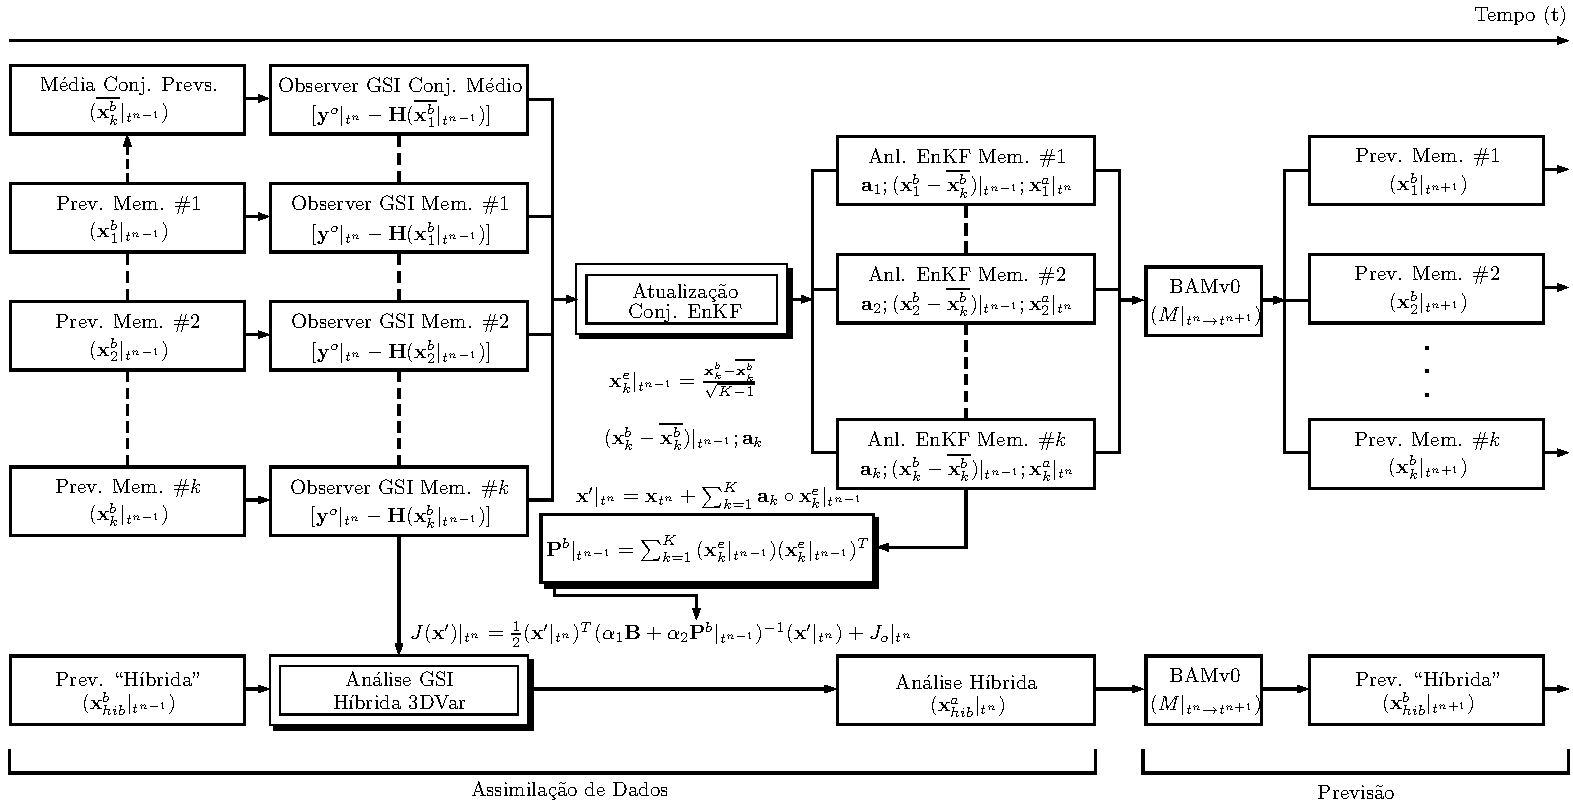
\includegraphics[width=\textwidth]{./docs/figs/diagrama_hibrido_novo_pt-tempos.pdf}
    \end{center}
\vspace{4mm}
\legenda{Um diagrama complexo com elementos geométricos e equações.}
\label{fig:ciclo}
\FONTE{Adaptado de \citeonline{bastarz/2017}.}
\end{figure}

\begin{marker}
A página \url{https://tug.org/PSTricks/main.cgi?file=index} apresenta muitos exemplos de desenhos feitos com o PS\textit{Tricks}.
\end{marker}

A utilização do programa \LaTeX\textit{Draw} é bastante simples. Na Figura \ref{fig:interld} mostra-se a interface principal do programa, onde pode-se ver o menu principal, a barra de ferramentas e a área em que os desenhos e diagramas podem ser feitos.

\begin{figure}[H]
\caption{Interface gráfica do programa \LaTeX\textit{Draw}}
\vspace{6mm}
    \begin{center}
        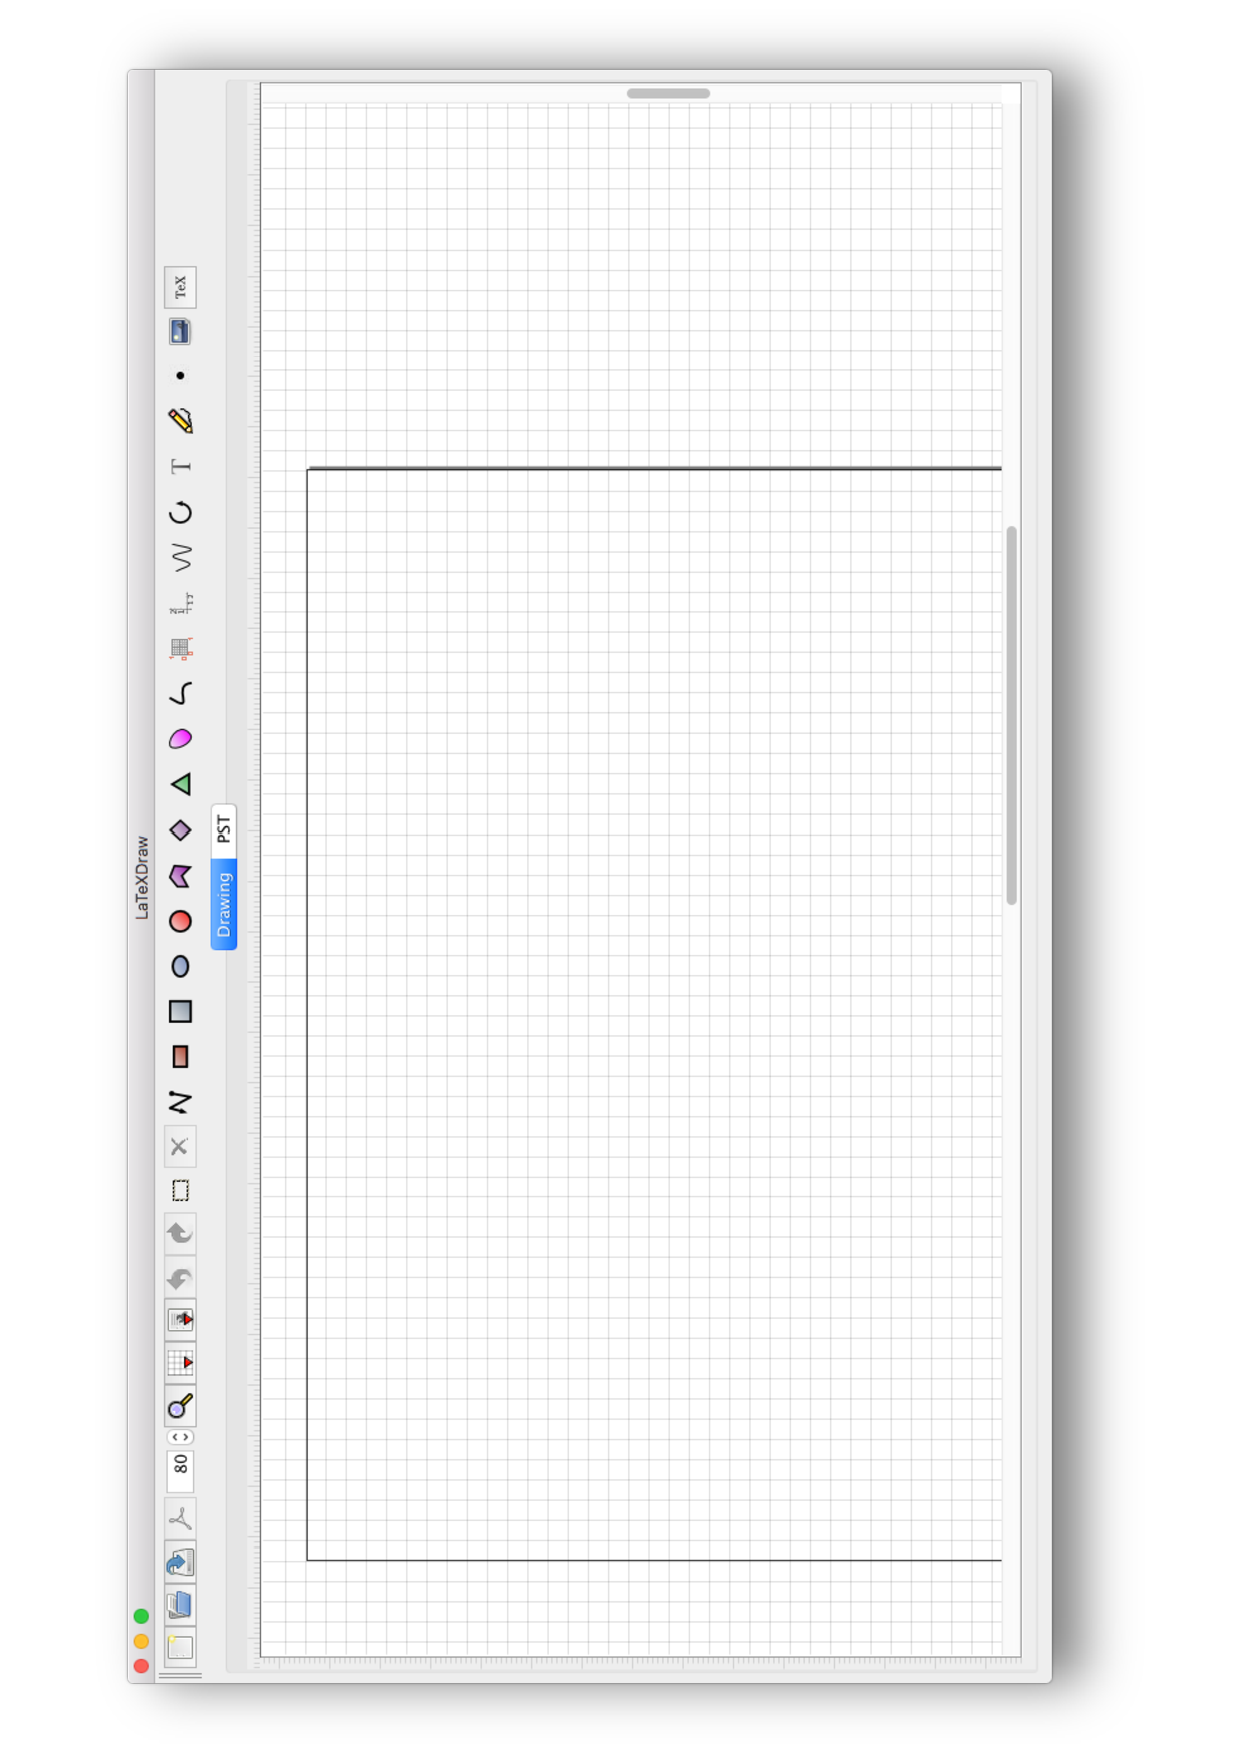
\includegraphics[width=0.7\textwidth,angle=-90]{./docs/figs/ldraw1.pdf}
    \end{center}
\vspace{4mm}
\legenda{Um programa para criação e diagramas e figuras simples.}
\label{fig:interld}
\FONTE{Produção do autor.}
\end{figure}

Na Figura \ref{fig:interld}, observe que há duas abas: \textit{Drawing} e ``PST''. Na aba \textit{Drawing}, é onde são feitos os desenhos. Utilizam-se as ferramentas de desenho disponíveis na barra de ferramentas, onde podem ser utilizadas as ferramentas de inserção de figuras geométricas e texto, incluindo equações (modo matemático do \LaTeX{}).

\begin{figure}[H]
\caption{Código PS\textit{Tricks} gerado pelo do programa \LaTeX\textit{Draw}}
\vspace{6mm}
    \begin{center}
        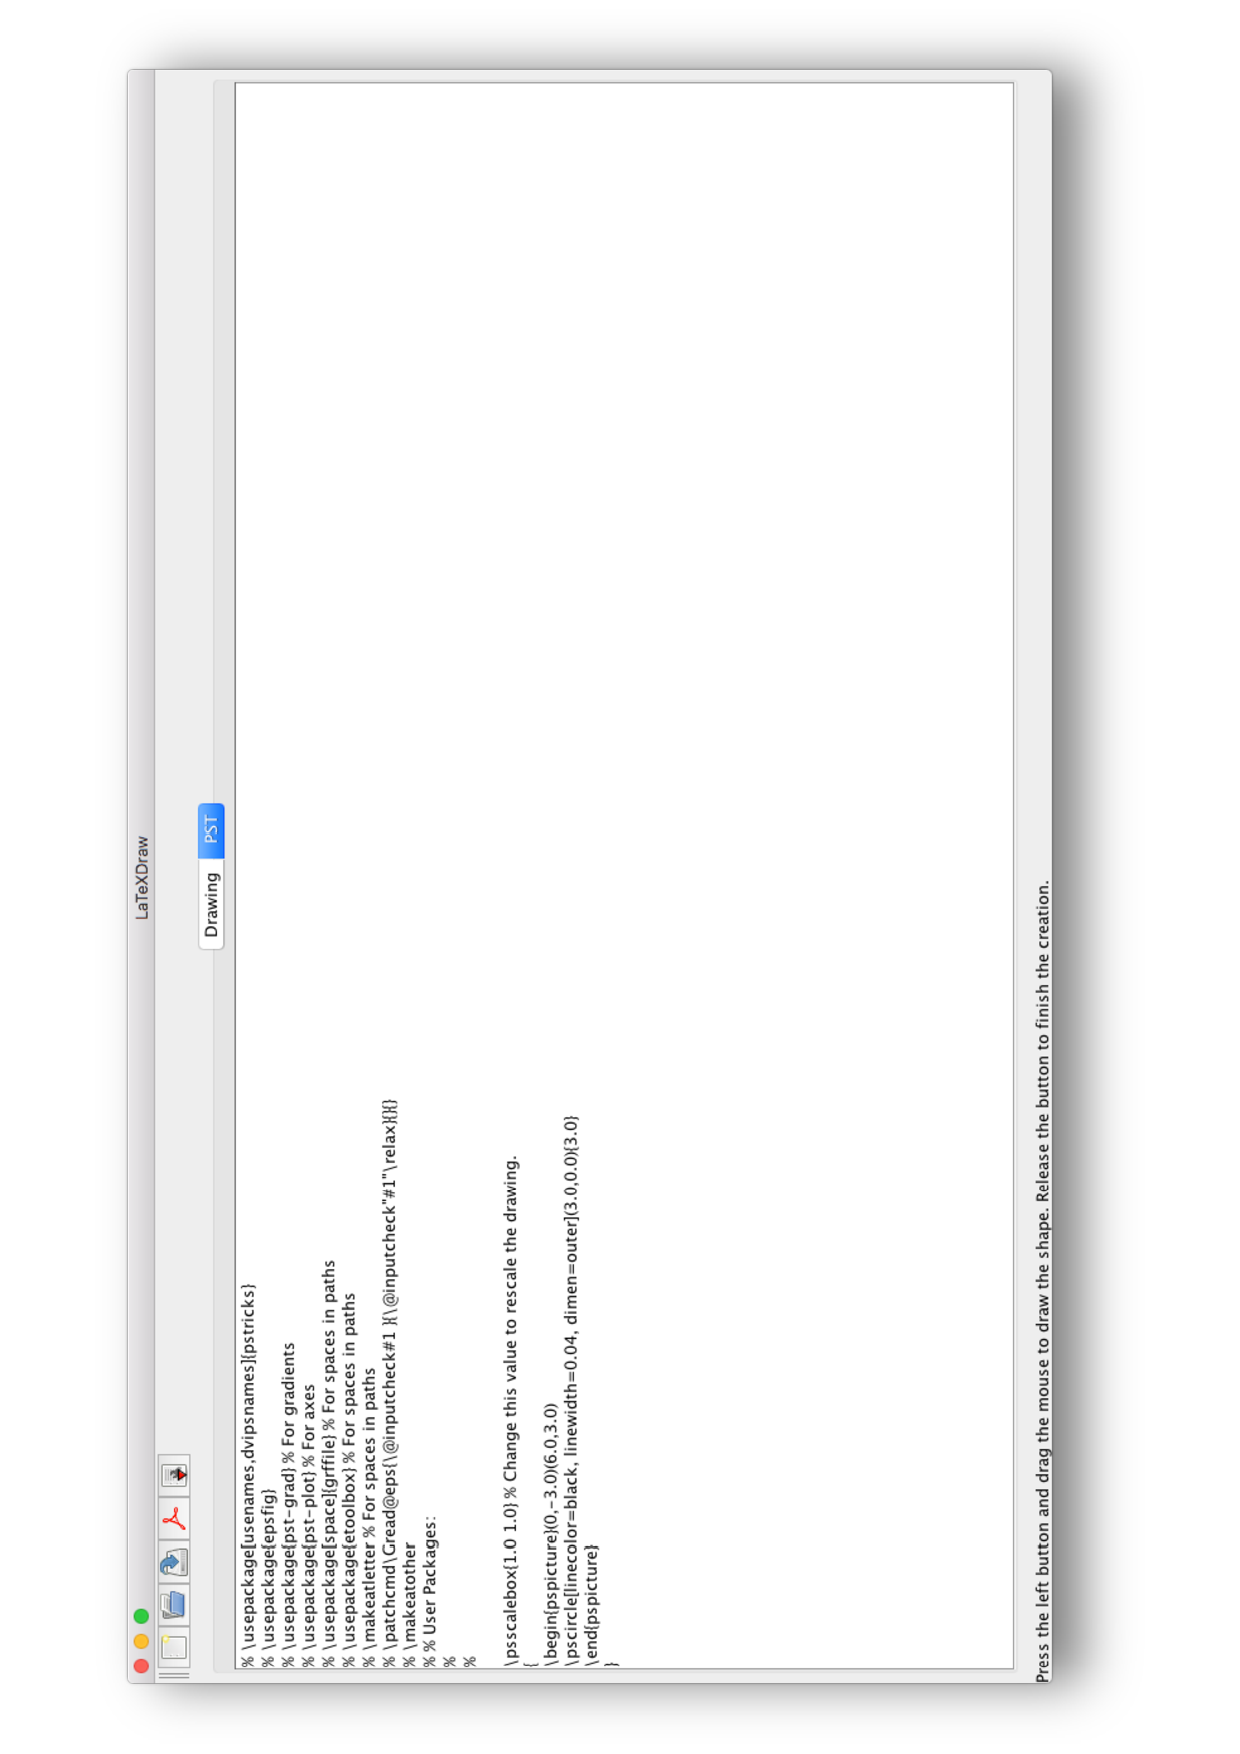
\includegraphics[width=0.7\textwidth,angle=-90]{./docs/figs/ldraw2.pdf}
    \end{center}
\vspace{4mm}
\legenda{Aba ``PST''.}
\label{fig:interld}
\FONTE{Produção do autor.}
\end{figure}

Na aba ``PST'', uma vez que algum desenho é inserido na aba \textit{Drawing}, pode-se obter o código PS\textit{Tricks} que gera o desenho inserido. Este código pode ser copiado para um arquivo \LaTeX{} (dentro de um ambiente apropriado), que pode então ser utilizado como fonte. A compilação do documento \LaTeX{} irá compilar e apresentar o desenho também dentro do corpo do texto. De forma convencional, pode-se exportar o desenho para um formato apropriado (e.g., PDF, PNG etc) e então inserir o desenho utilizando os ambientes apresentados na Seção \ref{sec:figuras}.

\begin{figure}[H]
\caption{Interface de exportação do programa \LaTeX\textit{Draw}}
\vspace{6mm}
    \begin{center}
        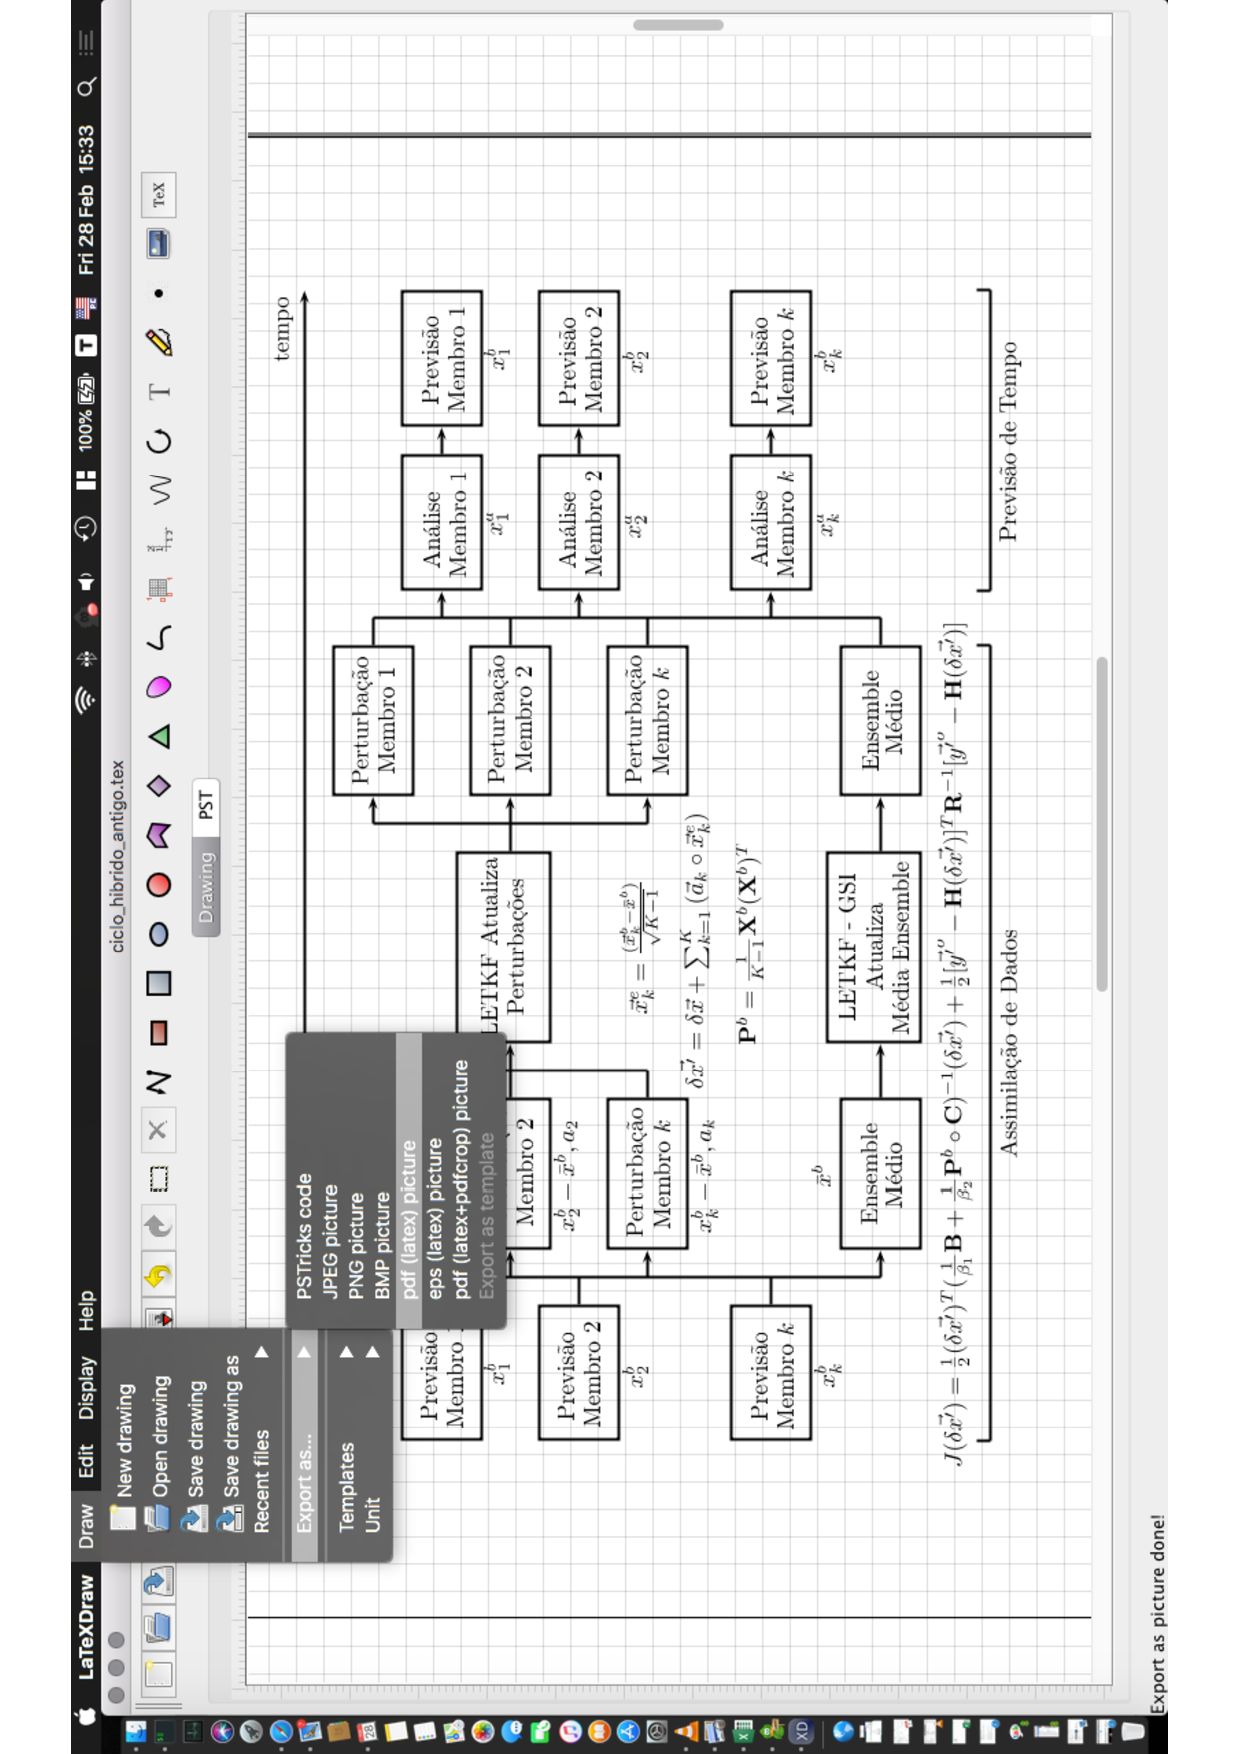
\includegraphics[width=0.7\textwidth,angle=-90]{./docs/figs/ldraw3.pdf}
    \end{center}
\vspace{4mm}
\legenda{Exportando uma figura para o formato PDF.}
\label{fig:interld}
\FONTE{Produção do autor.}
\end{figure}

\begin{marker}
Outro programa que também pode ser utilizado para a construção de figuras e diagramas é o Dia. Este programa também permite exportar os desenhos para os formatos PNG, PDF, EPS entre outros, além do próprio \LaTeX{} (como uma figura \textit{PSTricks}). Veja mais informações sobre o Dia em \url{http://dia-installer.de/}.
\end{marker}

\subsection{Matemática e equações}
\label{sec:mat_eqs}

O modo matemático do \LaTeX{} representa uma forma bastante conveniente de se inserir equações e símbolos matemáticos em um documento. Equações podem ser digitadas diretamente em parágrafos (em linha ou \textit{inline}) utilizando uma dupla de {\tt \$\$}'s (cifrões), {\tt []}'s (colchetes) ou \mintinline{latex}{()}'s (parênteses) como delimitadores. Por exemplo, equação $ax^2 + bx + c = 0$ pode ser digitada como \mintinline{latex}{$ax^2 + bx + c = 0$} no meio de uma frase ou parágrafo. Veja no Exempo \ref{exe_eq0} formas diferentes de digitar equações em linha.

\begin{texexptitled}[breakable,center lower,enhanced,middle=2mm]{Inserindo equações em linha (\textit{inline})}{exe_eq0}
Uma equação do segundo grau tem a forma geral, $ax^2 + bx + c =0$. Suas raízes são calculadas por, $x = \frac{-b \pm \sqrt{b^2 - 4ac}}{2a}$.
\\
Uma equação do segundo grau tem a forma geral, \(ax^2 + bx + c =0\). Suas raízes são calculadas por, \(x = \frac{-b \pm \sqrt{b^2 - 4ac}}{2a}\).
\\
Uma equação do segundo grau tem a forma geral, \[ax^2 + bx + c =0\]. Suas raízes são calculadas por, \[x = \frac{-b \pm \sqrt{b^2 - 4ac}}{2a}\].
\end{texexptitled}

No Exemplo \ref{exe_eq0}, observe que os delimitadores dados por colchetes ou parênteses precisam ser ``escapados'', i.e., é necessário adicionar uma \verb|\| (barra invertida) antes deles (e.g., \verb|\[| e \verb|\]| ou \verb|\(| e \verb|\)|). Além disso, quando são utilizados os colchetes, as equações em linha são escritas em uma linha própria e centralizada com o texto. O resultado obtido com a digitação de equações em linha utilizando os delimitadores indicados, apresenta as equações dentro da definição de altura da linha do texto. Para fazer com que esta limitação seja contornada e dar mais espaço ao ambiente de equações em linha, utiliza-se um par de delimitadores duplos \verb|$$|'s (dólar duplo). Veja o Exemplo \ref{exe_eq00} a seguir:

\begin{texexptitled}[breakable,center lower,enhanced,middle=2mm]{Inserindo equações em linha (\textit{inline)} com espaço vertical extra}{exe_eq00}
Uma equação do segundo grau tem a forma geral, $$ax^2 + bx + c =0$$. Suas raízes são calculadas por, $$x = \frac{-b \pm \sqrt{b^2 - 4ac}}{2a}$$.
\end{texexptitled}

No \LaTeX{} é possível inserir todos os símbolos relacionados às ciências. No Anexo B há uma lista destes símbolos, os quais podem ser utilizados para a realização dos exercícios da Seção \ref{sec:exercicios}.

Para digitar equações em blocos, há ambientes próprios para casos variados, os quais são mostrados a seguir.

\subsubsection*{Ambientes de equações}
\label{sec:amb_eqs}

Equações podem ter aspectos muito variados. Podem ser longas, ocupando uma ou mais linhas e podem conter símbolos diversos. No \LaTeX{}, o pacote {\tt amsmath} fornece uma série de ambientes apropriados para escrever expressões numéricas e equações de forma adequada. Para carregar este pacote, inclua o comando \mintinline{latex}{\usepackage{amsmath}} no preâmbulo do documento.

Uma simples equação pode ser inserida utilizando-se o ambiente {\tt equation}. No Exemplo \ref{exe_eq1}, observe a diferença entre os resultados obtidos com os ambientes {\tt equation} e {\tt equation*}.

\begin{texexptitled}[breakable,center lower,enhanced,middle=2mm]{Ambientes {\tt equation} e {\tt equation*}}{exe_eq1}
\begin{equation*}
x = \frac{-b \pm \sqrt{b^{2} - 4ac}}{2a}
\end{equation*}

\begin{equation}
x = \frac{-b \pm \sqrt{b^{2} - 4ac}}{2a}
\end{equation}
\end{texexptitled}

No Exemplo \ref{exe_eq1}, o ambiente {\tt equation*} evita que as equações sejam numeradas. Além disso, as equações são numeradas de acordo com a numeração da seção em que elas estiverem inseridas. %Neste caso, a Equação \ref{eq1} pertence à Seção \ref{sec:mat_eqs}.

Equações podem ser alinhadas pelo sinal de ``='' (ou qualquer outro sinal) dentro do ambiente {\tt split}. Veja no Exemplo \ref{exe_eq2} como aplicar o ambiente {\tt split}: 

\begin{texexptitled}[breakable,center lower,enhanced,middle=2mm]{Ambientes {\tt equation} e {\tt split}}{exe_eq2}
\begin{equation*}
\begin{split}
f(x) & = x^{-\frac{1}{2}}   \\
     & = \frac{1}{\sqrt{x}}\text{, }\forall x \neq 0.
\end{split}
\end{equation*}

\begin{equation}
\begin{split}
f(x) & = x^{-\frac{1}{2}}   \\
     & = \frac{1}{\sqrt{x}}\text{, }\forall x \neq 0.
\end{split}
\end{equation}
\end{texexptitled}

No exemplo anterior, além do modo matemático puro, foram inseridos também modos de texto com o marcador {\tt text}. Este marcador serve para digitar texto dentro do ambiente {\tt equation} (neste caso foi digitada uma vírgula acrescida de um espaço em branco, i.e., \mintinline{latex}{\text{, }}).

No Exemplo \ref{exe_eq3}, o ambiente {\tt multiline} é utilizado para inserir equações muito longas. Neste ambiente, pode-se escolher em que parte a equação deverá ser truncada utilizando-se um par de \verb|\\|'s (barras invertidas):

%P(x) = a_{n}x^{n} + a_{n-1}x^{n-1} + a_{n-2}x^{n-2} + a_{n-3}x^{n-3} 
%+ \cdots \\ + a_{3}x^{3} + a_{2}x^{2} + a_{1}x^{1} + a_{0}x^{0} 
%= \sum_{i=0}^{n}{a_{i}x^{i}}
\begin{texexptitled}[breakable,center lower,enhanced,middle=2mm]{Ambiente {\tt multline}}{exe_eq3}
\begin{multline*}
  A(x,y)\frac{\partial^2{\Psi}}{\partial{x^2}}           + 
  B(x,y)\frac{\partial^2{\Psi}}{\partial{x}\partial{y}}  +
  C(x,y)\frac{\partial^2{\Psi}}{\partial{y^2}}           +
  D(x,y)\frac{\partial{\Psi}}{\partial{x}}               + \\
+ E(x,y)\frac{\partial{\Psi}}{\partial{y}}               +
  F(x,y)\Psi = G(x,y)
\end{multline*}

\begin{multline}
  A(x,y)\frac{\partial^2{\Psi}}{\partial{x^2}}           + 
  B(x,y)\frac{\partial^2{\Psi}}{\partial{x}\partial{y}}  +
  C(x,y)\frac{\partial^2{\Psi}}{\partial{y^2}}           +
  D(x,y)\frac{\partial{\Psi}}{\partial{x}}               + \\
+ E(x,y)\frac{\partial{\Psi}}{\partial{y}}               +
  F(x,y)\Psi = G(x,y)
\end{multline}
\end{texexptitled}

Nos Exemplos \ref{exe_eq2} e \ref{exe_eq3}, observe que os ambientes {\tt split} e {\tt multline} funcionam de forma semelhante, com a diferença de que o ambiente {\tt split} deve ser utilizado dentro do ambiente {\tt equation}. Além disso, o ambiente {\tt split} alinha as equações como em uma tabela, i.e., com o símbolo \& (\textit{ampersand}) separando as colunas ou partes da equação.

Para alinhar equações ou grupos de equações, pode-se utilizar o ambiente {\tt align}. Veja os grupos de equações do Exemplo \ref{exe_eq4}:

\begin{texexptitled}[breakable,center lower,enhanced,middle=2mm]{Ambiente {\tt align}}{exe_eq4}
\begin{align*}
 x           & = 1 + 2y + 3z \\ 
3x -  y + 2z & = 0           \\
2x +  y      & = 2 - z
\end{align*}

\begin{align}
e^{i\pi} + 1 & = 0                                           \\
e & = \lim_{n \to \infty}{\Bigg(1 + \frac{1}{n}\Bigg)^{n}}   \\
y & = \sin 2\pi \Bigg(\frac{1}{2\pi}\sqrt{\frac{k}{m}}\Bigg)
\end{align}
\end{texexptitled}

No Exemplo \ref{exe_eq4}, observe também que foi utilizado o marcador {\tt Bigg} antes dos parênteses. Este marcador, no modo matemático, permite que parênteses, colchetes e chaves sejam ampliados de forma que se ajustem à altura dos símbolos das equações que estão sendo digitadas. Outros marcadores podem ser utilizados para ampliar estes sinais matemáticos na escala correta. Pode-se utilizar {\tt big} para produzir $x=\big(\frac{1}{25}\big)^{\frac{1}{2}}$, ou {\tt bigg} para produzir $x=\bigg(\frac{1}{25}\bigg)^{\frac{1}{2}}$, ou ainda {\tt Big} para produzir $x=\Big(\frac{1}{25}\Big)^{\frac{1}{2}}$ e {\tt Bigg} para se obter $x=\Bigg(\frac{1}{25}\Bigg)^{\frac{1}{2}}$.

\begin{marker}
Veja mais opções de marcadores especiais para o modo matemáticos em \url{https://www.overleaf.com/learn/latex/Brackets_and_Parentheses}.
\end{marker}

Equações podem ser alinhadas utilizando-se o ambiente {\tt gather}. Este alinhamento produz um resultado diferente daquele obtido com o ambiente {\tt align}. Veja no Exemplo \ref{exe_eq5} a seguir como utilizar o ambiente {\tt gather}:

\begin{texexptitled}[breakable,center lower,enhanced,middle=2mm]{Ambiente {\tt gather}}{exe_eq5}
\begin{gather*}
 x           = 1 + 2y + 3z \\ 
3x -  y + 2z = 0           \\
2x +  y      = 2 - z
\end{gather*}

\begin{gather}
 x           = 1 + 2y + 3z \\ 
3x -  y + 2z = 0           \\
2x +  y      = 2 - z
\end{gather}
\end{texexptitled}

Com o ambiente {\tt gather}, as equações são alinhadas em relação ao parágrafo, e não com relação a um elemento. Outros elementos matemáticos como sinais e símbolos em geral podem ser encontrados nas tabelas do Anexo B.

\subsection{Tabelas}
\label{sec:tabs}

Tabelas são os elementos do texto que resumem e organizam informações. No \LaTeX{}, tabelas são escritas em ambientes específicos, que podem, dependendo da necessidade, ajustar automaticamente o seu conteúdo aos limites das dimensões do texto. Antes de apresentar os ambientes mais comuns de tabelas, salienta-se que a construção de tabelas pode se tornar uma tarefa um pouco mais complicada do que parece, principalmente se a tabela em questão possuir muitas células mescladas. Portanto, recomenda-se a construção tabelas simples e clara.

O ambiente {\tt tabular} é um ambiente simples para a construção de tabelas. A sua utilização é apresentada no Exemplo \ref{exe_tab1}.

\begin{texexptitled}[breakable,center lower,enhanced,middle=2mm]{Exemplo de uma tabela simples com o ambiente {\tt tabular}}{exe_tab1}
\begin{tabular}{c c}
\hline 
\textbf{L0C1} & \textbf{L0C2} \\
\hline
L1C1 & L1C2 \\
L2C1 & L2C2 \\
L3C1 & L3C2 \\
L4C1 & L4C2 \\
L5C1 & L5C2 \\
\hline
\end{tabular}
\end{texexptitled}

Na tabela do Exemplo \ref{exe_tab1}, tem-se apenas duas colunas e algumas linhas. Para separar o conteúdo, utilizou-se apenas linhas horizontais (produzidas pelos comandos {\tt hline}) para separar o cabeçalho, i.e., os nomes das colunas, do conteúdo. Observe que a tabela produzida possui as linhas muito próximas, e este espaçamento pode ser melhorarado com a utilização do comando \mintinline{latex}{\\[-0.5em]}. Lembre-se que a instrução \mintinline{latex}{\\} pula uma linha; o argumento desta instrução, i.e., \mintinline{latex}{[-0.5em]} indica que o espaço de uma linha deve ser recuado em {\tt -0.5em}. Na Tabela \ref{tab:medidas} está indicado que a unidade {\tt em} refere-se à altura do caractere ``M'' da fonte em uso, isso garante que o espaçamento será sempre consistente independente do estilo da fonte em uso. Veja o Exemplo \ref{exe_tab2} a seguir:

\begin{texexptitled}[breakable,center lower,enhanced,middle=2mm]{Exemplo de uma tabela simples com o ambiente {\tt tabular} e linhas mais altas}{exe_tab2}
\begin{tabular}{l r}
\hline 
\\[-0.5em]
\textbf{L0C1} & \textbf{L0C2} \\
\\[-0.5em]
\hline
\\[-0.5em]
L1C1 & L1C2 \\
\\[-0.5em]
L2C1 & L2C2 \\
\\[-0.5em]
L3C1 & L3C2 \\
\\[-0.5em]
L4C1 & L4C2 \\
\\[-0.5em]
L5C1 & L5C2 \\
\\[-0.5em]
\hline
\end{tabular}
\end{texexptitled}

No Exemplo \ref{exe_tab2}, observe a instrução \mintinline{latex}{{l r}}. Como a tabela do exemplo possui apenas duas colunas, indica-se com um par de colchetes o seu alinhamento, logo após o início do ambiente {\tt tabular}. Neste caso, o conteúdo da coluna da esquerda encontra-se alinhado à esquerda, enquanto que o conteúdo da coluna da direita, encontra-se alinhado à direita (por isso {\tt l r}). Isto deve ser feito para a quantidade de colunas que a tabela possuir. Se uma tabela no ambiente {\tt tabular}, possuir 5 colunas, deve-se especificar o alinhamento desejado para as colunas, e.g., \mintinline{latex}{{l r l l c}}. Portanto, para alinhar o conteúdo à esquerda, utilize {\tt l} (do inglês \textit{left}), para alinhar à direita utilize {\tt r} (do inglês \textit{right}) e para centralizar o conteúdo (tal como no Exemplo \ref{exe_tab1}), utilize {\tt c} (do inglês \textit{center}).

Além de alterar o espaçamento vertical dentro de uma tabela, pode-se também alterar a largura das colunas. Para isso, pode-se utilizar o comando \mintinline{latex}{p{u.}}, onde {\tt u.} corresponde a alguma medida. Veja o Exemplo \ref{exe_tab3} a seguir:

\begin{texexptitled}[breakable,center lower,enhanced,middle=2mm]{Exemplo de uma tabela simples com o ambiente {\tt tabular} e colunas mais largas}{exe_tab3}
\begin{tabular}{p{3cm}  p{5cm}}
\hline 
\\[-0.5em]
\textbf{L0C1} & \textbf{L0C2} \\
\\[-0.5em]
\hline
\\[-0.5em]
L1C1 & L1C2 \\
\\[-0.5em]
L2C1 & L2C2 \\
\\[-0.5em]
L3C1 & L3C2 \\
\\[-0.5em]
L4C1 & L4C2 \\
\\[-0.5em]
L5C1 & L5C2 \\
\\[-0.5em]
\hline
\end{tabular}
\end{texexptitled}

\begin{marker}
No Exemplo \ref{exe_tab3}, o conteúdo das colunas foi marcado como {\tt p} (do inglês \textit{paragraph}). Nessa forma mais simples de se especificar a largura das colunas, não é possível posicionar o texto de outra forma, i.e., centralizado ou alinhado à direita ou esquerda.
\end{marker}

Assim como as tabelas produzidas em editores WYSIWYG, no \LaTeX{} também é possível mesclar células (na direção das colunas ou das linhas). Para isso, utilizam-se os comandos \mintinline{latex}{\multicolumn} para mesclar colunas e \mintinline{latex}{\multirow} para mesclar linhas. Veja o Exemplo \ref{exe_tab4} a seguir:

\begin{texexptitled}[breakable,center lower,enhanced,middle=2mm]{Exemplo de uma tabela simples com o ambiente {\tt tabular} e células mescladas com o comando {\tt multirow}}{exe_tab4}
\begin{tabular}{|p{3cm}|p{3cm}|p{3cm}|p{3cm}|}
\hline
\multicolumn{4}{|c|}{4 Células Mescladas (colunas)} \\
\hline
\multicolumn{2}{|c|}{2 Células Mescladas (colunas)} &
\multicolumn{2}{c|}{2 Células Mescladas (colunas)} \\
\hline 
\multicolumn{1}{|c|}{Coluna 1} & 
\multicolumn{1}{c|}{Coluna 2} & 
\multicolumn{1}{c|}{Coluna 3} & \multicolumn{1}{c|}{Coluna 4} \\
\hline
\lipsumsentence[1-2] & \lipsumsentence[3-4] & \lipsumsentence[5-6] & 
\lipsumsentence[7-8] \\
\hline
\end{tabular}
\end{texexptitled}

Na tabela do Exemplo \ref{exe_tab4}, tem-se uma tabela mais complexa, em que colunas estão mescladas de formas diferentes. Além disso, diferentemente dos exemplos anteriores, a tabela apresentada possui limitadores verticais que são desenhados utilizando-se o símbolo {\tt |} (\textit{pipe})\footnote{Pode-se também utilizar \textit{pipes} duplos.}, como argumento do comando que inicia o ambiente \mintinline{latex}{tabular}: {\tt |p{3cm}|p{3cm}|p{3cm}|p{3cm}|}. Observe também que a tabela desenhada possui o total de quatro colunas, cujas larguras podem ser especificadas (no exemplo, cada uma com {\tt 3cm}). Outro detalhe a ser observado neste exemplo, é a forma como o conteúdo é alinhado dentro das células. Neste caso, o alinhamento é dado por um argumento do comando \mintinline{latex}{multicolumn}: \mintinline{latex}{{4}{|c|}}, onde 4 indica a quantidade de células a serem mescladas e \mintinline{latex}{|c|} indica que o conteúdo das células a serem mescladas será centralizado e delimitado por \textit{pipes} nos limites laterais da célula.

\subsubsection*{Tabelas ajustáveis}
\label{sec:amb_tabs}

Dependendo da necessidade, ambientes especiais de tabelas podem ser necessários. Alguns ambientes de tabelas mais comuns são {\tt tabular}, {\tt tabularx} e {\tt booktabs}, os quais possuem características e propriedades específicas.

% REF: https://tex.stackexchange.com/questions/341205/what-is-the-difference-between-tabular-tabular-and-tabularx-environments/341212

Tabelas ajustáveis podem ser necessárias quando se deseja que a largura das colunas sejam automaticamente ajustadas. No caso do ambiente {\tt tabular}, o \LaTeX{} tenta ajustar a largura da tabela de acordo com a quantidade de informações contida nas células. Se as células contiverem muita informação, a tabela poderá ficar com uma largura maior do que a largura do texto ou mesmo da página. Veja no Exemplo \ref{exe_tab5} a utilização básica do ambiente {\tt tabular}.

%Com relação ao ambiente {\tt tabular}, tem-se duas variações do mesmo, os ambientes {\tt tabular*} e o {\tt tabularx}. A diferença entre eles está na forma como a largura da tabela é ajustada com relação ao texto. Observe o Exemplo \ref{exe_tab5} a seguir que a tabela gerada com o ambiente {\tt tabular} não possui largura fixa e ela se ajusta à quantidade de conteúdo, tendo como limite a largura do parágrafo onde estiver inserida.

\begin{texexptitled}[breakable,center lower,enhanced,middle=2mm]{Exemplo de uma tabela simples utilizando o ambiente {\tt tabular}}{exe_tab5}
\begin{tabular}{|l|c|r|}
\hline
L1C1 L1C1 L1C1 L1C1 & L1C2 L1C2 L1C2 L1C2 L1C2 L1C2 & L1C3      \\
L2C1 L2C1 L2C1 L2C1 & L2C2 L2C2 L2C2 L2C2 L2C2 L2C2 & L2C3 L2C3 \\
\hline
\end{tabular}
\end{texexptitled}

No Exemplo \ref{exe_tab5} a quantidade de informação nas células não é suficiente para fazer com que a largura da tabela extrapole os limites da página, mas isto é perfeitamente possível dentro do ambiente {\tt tabular}. Para evitar esta situação, o ambiente {\tt tabularx} é mais apropriado, visto que com ele pode-se definir uma largura fixa (por meio de um valor ou de uma \textit{macro}) e o conteúdo das células é ajustado dentro destes limites. No Exemplo \ref{exe_tab7} mostra-se o que se obtém com a utilização do ambiente {\tt tabularx}.

%Já no Exemplo \ref{exe_tab6}, a tabela gerada com o ambiente {\tt tabular*} possui largura fixa, e o seu limite é a largura do parágrafo no qual está inserida (por isso o marcador {\tt textwidth}). Observe que o conteúdo da tabela se ajusta à largura fixa. Além disso, no exemplo está indicado o marcador \mintinline{latex}{@{\extracolsep{\fill}}}, o qual permite que o próprio \LaTeX{} decida como o conteúdo das células serão acomodados dentro da largura fixada. Uma aplicação mais clara sobre o funcionamento de uma tabela com largura ajustável (em inglês o termo seria \textit{rubber length}), é mostrado no Exemplo \ref{exe_tab6} a seguir.

%\begin{texexptitled}[breakable,center lower,enhanced,middle=2mm]{Exemplo de uma tabela simples  utilizando o ambiente {\tt tabular*}}{exe_tab6}
%\begin{tabular*}{\textwidth}{@{\extracolsep{\fill}}|l|c|r|}
%\hline
%L1C1 & L1C2 & L1C3 \\
%L2C1 & L2C2 & L2C3 \\
%\hline
%\end{tabular*}
%
%\begin{tabular*}{0.75\textwidth}{@{\extracolsep{\fill}} | c | c | c | r | }
%\hline
%label 1 & label 2 & label 3 & label 4 \\
%\hline 
%item 1  & item 2  & item 3  & item 4  \\
%\hline
%\end{tabular*}
%\end{texexptitled}

%\begin{texexptitled}[breakable,center lower,enhanced,middle=2mm]{Exemplo de uma tabela simples  utilizando o ambiente {\tt tabular*}}{exe_tab6}
%\begin{tabular*}{\textwidth}{@{\extracolsep{\fill}}|l|c|r|}
%  \hline
%  L1C1 & L1C2 & L1C3 \\
%  L2C1 & L2C2 & L2C3 \\
%  \hline
%\end{tabular*}
%\end{texexptitled}

%O Exemplo \ref{exe_tab7} a seguir, utiliza o ambiente {\tt tabularx} que permite deixar as colunas da tabela com tamanhos iguais, além de possuir largura total fixa com limite relativo à largura do parágrafo (assim como o ambiente {\tt tabular*}):

\begin{texexptitled}[breakable,center lower,enhanced,middle=2mm]{Exemplo de uma tabela simples utilizando o ambiente {\tt tabularx}}{exe_tab7}
\begin{tabularx}{\textwidth}{|X|X|X|}
\hline
L1C1 L1C1 L1C1 L1C1 & L1C2 L1C2 L1C2 L1C2 L1C2 L1C2 & L1C3      \\
L2C1 L2C1 L2C1 L2C1 & L2C2 L2C2 L2C2 L2C2 L2C2 L2C2 & L2C3 L2C3 \\
\hline
\end{tabularx}
\end{texexptitled}

% FALTA: colorir células e fontes dentro das células e a espessura/estilo das linhas das tabelas

No Exemplo \ref{exe_tab7}, as colunas da tabela estão ajustadas com a mesma largura. Isso é possível através da opção {\tt X}, utilizada como opção do comando {\tt tabularx}, como em \mintinline{latex}{\begin{tabularx}{\textwidth}{|X|X|X|}}.

O pacote {\tt booktabs} permite utilizar linhas mais grossas através dos marcadores \mintinline{latex}{\toprule}, \mintinline{latex}{\midrule} e \mintinline{latex}{\bottomrule}. Para utilizar o pacote, é necessário carregá-lo no preâmbulo do documento com o comando \mintinline{latex}{\usepackage{booktabs}}. Veja o Exemplo \ref{exe_tab8} a seguir e compare o resultado com as tabelas dos exemplos anteriores que utilizaram o marcador \mintinline{latex}{\hline} para separar as linhas das tabelas:

% REF: https://texblog.org/2017/02/06/proper-tables-with-latex/

\begin{texexptitled}[breakable,center lower,enhanced,middle=2mm]{Exemplo de uma tabela simples utilizando o ambiente {\tt tabular} e os marcadores {\tt toprule}, {\tt midrule} e {\tt bottomrule}}{exe_tab8}
\begin{tabular}[t]{lcc}
\toprule
     & L1C2 & L1C3 \\
\midrule
L2C1 & L2C2 & L2C3 \\
L3C1 & L3C2 & L3C3 \\
L4C1 & L4C2 & L4C3 \\
\bottomrule
\end{tabular}
\end{texexptitled}

% Dicas úteis para estilizar tabelas: https://inf.ethz.ch/personal/markusp/teaching/guides/guide-tables.pdf

Os ambientes {\tt tabular} e {\tt tabularx} possuem algum controle sobre a largura da tabela de acordo com a quantidade de informação dentro das células. Por outro lado, tabelas muito longas, e.g., que podem ocupar várias páginas, podem não ser adequadamente acomodadas com estes ambientes. Para isso, recomenda-se a utilização do pacote {\tt longtable} que permite o \LaTeX{} realizar a quebra automática de linha dentro de uma tabela. Considere o Exemplo \ref{ltable1} a seguir, em que uma tabela longa é inserida dentro de um ambiente {\tt tabularx}:

\begin{texexptitled}[center lower,enhanced jigsaw,middle=2mm,lower separated=true, listing side comment,righthand width=4cm,compilable listing,run latex,run dvips,run ps2pdf,pdf comment,comment style={raster columns=1}, freeze pdf]{Uma tabela longa utilizando o ambiente {\tt tabularx}}{ltable1}
\documentclass{article}
\usepackage[utf8]{inputenc}
\usepackage{tabularx}
\usepackage{lipsum}

\title{Título}
\author{Nome}
\date{\today}

\begin{document}

\maketitle

\section{Seção}

\lipsum[1]

\begin{tabularx}{\textwidth}{|X|X|}
\hline
Coluna 1     & Coluna 2     \\
\hline
\lipsum[1-2] & \lipsum[1-2] \\
\hline
\lipsum[1-2] & \lipsum[1-2] \\
\hline
\end{tabularx}

\lipsum[2]

\end{document}
\end{texexptitled}

Compare o Exemplo \ref{ltable1} com o Exemplo \ref{ltable2} a seguir, em que a mesma tabela longa é apresentada, porém com o auxílio do pacote {\tt longtable}.

\begin{texexptitled}[breakable,center lower,enhanced jigsaw,middle=2mm,lower separated=true, listing side comment,righthand width=4cm,compilable listing,run latex,run dvips,run ps2pdf,pdf comment,comment style={raster columns=1}, freeze pdf]{Uma tabela longa utilizando o ambiente {\tt longtable}}{ltable2}
\documentclass{article}

\usepackage[utf8]{inputenc}
\usepackage{lipsum}
\usepackage{longtable}

\title{Título}
\author{Nome}
\date{\today}

\begin{document}

\maketitle

\section{Seção}

\lipsum[1]

\begin{center}
\begin{longtable}{
  @{\extracolsep{\fill}}|p{6cm}|p{6cm}|
}
\hline
\textbf{Coluna 1} & \textbf{Coluna 2} \\
\hline
\endfirsthead
\multicolumn{2}{c}
{\tablename\ \thetable\ -- Continuação} \\
\hline
\textbf{Coluna 1} & \textbf{Coluna 2} \\
\hline
\endhead
\hline \multicolumn{2}{r}{(Continua)} \\
\endfoot
\hline
\endlastfoot
\lipsum[1-2] & \lipsum[1-2] \\
\hline
\lipsum[1-2] & \lipsum[1-2] \\
\end{longtable}
\end{center}

\end{document}
\end{texexptitled}

Seguindo o código apresentado no Exemplo \ref{ltable2}, pode-se confeccionar as Tabelas \ref{tab:pacotes} e \ref{tab:pacotes_uteis} do Apêndice A.

\begin{marker}
Editores \textit{online} podem ser utilizados para construir tabelas simples no \LaTeX{}. Observe que tabelas muito complexas podem ser difíceis de manipular e atualizar. Veja os \textit{sites} \url{https://www.tablesgenerator.com/} e \url{https://www.latex-tables.com} para mais informações.
\end{marker}

\subsection{Ferramentas de revisão}
\label{sec:ferrev}

A colaboração entre várias pessoas na escrita de um documento, pode mostrar-se como um verdadeiro desafio. Mesmo utilizando editores do tipo WYSIWYG, como o \textit{Microsoft Word}, unificar as diferentes versões de um documento por ser uma tarefa confusa e que certamente irá consumir muito tempo. Para isto, pode-se recorrer a ferramentas de revisão mais elaboradas como o \textit{track changes}, que permite rastrear as modificações feitas em um documento. Mas para a escrita com a linguagem \LaTeX{}, esta tarefa não é exatamente igual. Editores \textit{online}, como o \href{https://www.overleaf.com/}{\textit{Overleaf}}, são muito úteis e eficientes quanto à revisão, histório do documento e escrita colaborativa. Mas para editores locais, é possível utilizar alguns pacotes que irão habilitar a utilização da linguagem para a revisão, de forma semelhante ao que ocorre com editores WYSIWYG.

O pacote {\tt todonotes}, pode ser utilizado nesta tarefa. Com ele é possível inserir notas coloridas no documento de forma que se possa chamar a atenção para alguma parte do texto. Veja o Exemplo \ref{todo1} a seguir com a sua utilização.

%\begin{texexptitled}[center lower,enhanced jigsaw,middle=2.2mm,lower separated=true, listing side comment,righthand width=4cm,compilable listing,run latex,run dvips,run ps2pdf,pdf comment,comment style={raster columns=1}, freeze pdf]{Inserindo notas coloridas no texto com o pacote {\tt todonotes}}{todo1}
%\documentclass{article}
%
%\usepackage[utf8]{inputenc}
%\usepackage{xargs}
%\usepackage{xcolor-material}
%
%\usepackage[colorinlistoftodos,
%            prependcaption,
%            textsize=tiny]{todonotes}
%
%\newcommandx{\reescrever}[2][1=]{
%  \todo[linecolor=MaterialRed,
%  backgroundcolor=MaterialRed!25,
%  bordercolor=MaterialRed,#1]{#2}
%}
%\newcommandx{\verificar}[2][1=]{
%  \todo[linecolor=MaterialBlue,
%  backgroundcolor=MaterialBlue!25,
%  bordercolor=MaterialBlue,#1]{#2}
%}
%\newcommandx{\comentario}[2][1=]{
%  \todo[linecolor=MaterialGreen,
%  backgroundcolor=MaterialGreen!25,
%  bordercolor=MaterialGreen,#1]{#2}
%}
%\newcommandx{\remover}[2][1=]{
%  \todo[disable,#1]{#2}
%}
%
%\title{Meu documento}
%\author{Meu Nome}
%\date{\today}
%
%\begin{document}
%
%\maketitle
%
%Este é um exemplo de texto com notas coloridas.\reescrever{Este é um exemplo simples de texto com notas coloridas, utilizando o pacote todonotes.}
%
%\end{document}
%\end{texexptitled}

\begin{texexptitled}[center lower,enhanced jigsaw,middle=2mm,lower separated=true, listing side comment,righthand width=5cm,compilable listing,run latex,run dvips,run ps2pdf,pdf comment,comment style={raster columns=1}, freeze pdf]{Inserindo notas coloridas no texto com o pacote {\tt todonotes}}{todo1}
\documentclass{article}

\usepackage[utf8]{inputenc}
\usepackage{xargs}
\usepackage{xcolor-material}
\usepackage{lipsum}

\usepackage{todonotes}

\newcommandx{\minhanotaA}[2][1=]{
  \todo[linecolor=MaterialAmber,
  backgroundcolor=MaterialAmber!25,
  bordercolor=MaterialAmber,#1]{#2}
}

\newcommandx{\minhanotaV}[2][1=]{
  \todo[linecolor=MaterialGreen,
  backgroundcolor=MaterialGreen!25,
  bordercolor=MaterialGreen,#1]{#2}
}

\title{Meu documento}
\author{Meu Nome}
\date{\today}

\begin{document}

\maketitle

\lipsum[1]\minhanotaA{Esta é uma nota colorida.}
\lipsum[2]\minhanotaV{Esta é uma outra nota colorida.}

\end{document}
\end{texexptitled}

No Exemplo \ref{todo1}, observe que, além dos pacotes {\tt inputenc} e {\tt xcolor-material} (os quais fornecem suporte à acentuação e a paleta de cores \textit{Material Design} do Google, respectivamente), foi necessário também carregar os pacotes {\tt xargs} e {\tt todonotes}. O pacote {\tt xargs} permite a definição de comandos utilizando-se múltiplos argumentos. O pacote {\tt todonotes} é o que fornece a interface necessária para a inserção das notas personalizadas. Além disso, observe também que forma definidos dois comandos (duas \textit{macro}) de nomes {\tt minhanotaA} e {\tt minhanotaB}, os quais recebem um argumento que, de fato, é a nota que será inserida no texto. Na definição do comando {\tt minhanota}, foram ajustadas as seguintes opções: {\tt linecolor}, {\tt backgroundcolor} e {\tt bordercolor}. Estas opções fazem referência ao aspecto que as notas inseridas terão. Neste caso, escolheu-se a cor \textit{MaterialAmber} para a nota (uma variação da cor Ambar), fornecida pelo pacote {\tt xcolor-material}. Observe também que a cor atribuída à opção {\tt backgroundcolor} está definida como \mintinline{latex}{backgroundcolor=MaterialAmber!25}, i.e., da saturação total (100\%) da cor natural, removeu-se 25\%. Logo, o modificador {\tt !25}, indica a transparência de 25\% na aplicação da cor escolhida (mais opções de cores e paletas de cores podem ser encontradas na Seção \ref{sec:pal_cores}).

O pacote {\tt todonotes} permite a criação alguns tipos diferentes de notas. Pode-se, por exemplo, inserir notas que ocupam toda a largura do texto ou mesmo notas que não aparecem no texto. Pode-se também inserir um sumário com as notas, o que pode ser especialmente útil quando muitas notas de diferentes tipos são adicionadas. Veja o Exemplo \ref{todo2} a seguir com várias notas diferentes e um sumário de notas (este exemplo é baseado no exemplo encontrado \url{https://tex.stackexchange.com/questions/9796/how-to-add-todo-notes}).

\begin{texexptitled}[center lower,enhanced jigsaw,middle=2.2mm,lower separated=true, listing side comment,righthand width=4cm,compilable listing,run latex,run dvips,run ps2pdf,pdf comment,comment style={raster columns=1}, freeze pdf]{Inserindo notas coloridas no texto com o pacote {\tt todonotes}}{todo2}
\documentclass{article}

\usepackage[utf8]{inputenc}
\usepackage{xargs}
\usepackage{lipsum}

\usepackage{xcolor-material}
\usepackage[colorinlistoftodos,
            prependcaption,
            textsize=tiny]{todonotes}
            
\newcommandx{\comentario}[2][1=]{
  \todo[linecolor=MaterialAmber,
  backgroundcolor=MaterialAmber!25,
  bordercolor=MaterialAmber,#1]{#2}
}
\newcommandx{\remover}[2][1=]{
  \todo[linecolor=MaterialGreen,
  backgroundcolor=MaterialGreen!25,
  bordercolor=MaterialGreen,#1]{#2}
}

\title{Meu documento}
\author{Meu Nome}
\date{\today}

\begin{document}
\maketitle
\listoftodos[Notas]
\newpage
\lipsum[1]\comentario[inline]{Este é um comentário em em linha, o qual pode ser útil quando o comentário for muito grande com notas coloridas. Notas podem ser inseridas de formas diferentes. No entando, pode ser um pouco difícil de se acostumar.}

\lipsum[2]\comentario{Isso é verdade, principalmente quando não se está acostmado com o \LaTeX{}. Mas esta é uma boa opção, especialmente porque é o \LaTeX{} quem controla a aparição das notas.}

\lipsum[3]\remover{Remover esta parte!}
\end{document}
\end{texexptitled}

No Exemplo \ref{todo2}, observe que foram passadas opções para o pacote {\tt todonotes}. Estas opções foram fornecidas junto com o comando {\tt usepackage}. A primeira opção, {\tt colorlistoftodos}, permite a criação de uma lista de notas, tal como um sumário; a segunda opção, {\tt textsize=tiny}, ajusta o tamanho do texto dentro da nota para o tamanho {\tt tiny} (veja mais opções de tamanho de fontes na Seção \ref{sec:estilos}). A inserção das notas criadas é simples, bastando digitar o comando definido junto com o texto que será inserido na nota, e.g., \mintinline{latex}{\comentario{Meu comentário.}}. Para inserir uma nota em linha, i.e., uma nota que ocupa toda a largura do texto (especialemnte útil quando o texto da nota ocupar várias linhas), pode-se usar a opção {\tt inline} junto com o comando definido, e.g., \mintinline{latex}{\comentatio[inline]{Meu comentário muito longo escrito em linha.}}. Por fim, uma lista com as notas pode ser inserida com o comando \mintinline{latex}{\listoftodos[Nome da Lista]}. Este comando pode ser inserido em qualquer parte do texto. Conheça mais sobre o pacote {\tt todonotes} no site do CTAN em \url{https://www.ctan.org/pkg/todonotes}.

\begin{marker}
Veja também o pacote {\tt cooltooltips} no site do CTAN em \url{https://ctan.org/pkg/cooltooltips}. Este pacote fornece uma forma diferente de inserir comentários dentro de um documento \LaTeX{}.
\end{marker}

\subsection{Outros ambientes}
\label{sec:out_ambs}

O \LaTeX{} possui uma série de outros ambientes com os quais é possível apresentar e posicionar diferentes elementos textuais. É possível criar elementos flutuantes e posicioná-los em diferentes partes de uma página, bem como subdividir parágrafos em colunas, além de destacar as palavras reservadas de uma determinada linguagem de programação, incluindo os próprios comandos do \LaTeX{}. Nas subseções a seguir, serão apresentados alguns destes ambientes.

\subsubsection*{Minipage}
\label{sec:minipage}

Dependendo do tipo de documento escrito e dos elementos textuais utilizados, como imagens e tabelas, pode-se fazer necessário alocar tais elementos em posições específicas dentro da página. Para isto, pode-se utilizar o ambiente {\tt minipage}. Veja o Exemplo \ref{exe:minipage} a seguir sobre a sua utilização.

\begin{texexptitled}[breakable,enhanced,middle=2mm]{Texto em um ambiente {\tt minipage}}{exe:minipage}
\lipsum[1]

\begin{minipage}{0.5\textwidth}

\lipsum[2]

\end{minipage}

\lipsum[3]
\end{texexptitled}

No Exemplo \ref{exe:minipage}, observe que foi inserido um parágrafo dentro do ambiente {\tt minipage} de forma que este parágrafo possuísse apenas 50\% do tamanho da largura total de uma parágrafo da página. 

\subsubsection*{Texto em colunas}
\label{sec:colunas}

Texto e outros elementos flutuantes do \LaTeX{} podem ser inseridos no corpo do texto em colunas. Para isto, pode-se utilizar o pacote {\tt multicol}, que fornece o ambiente {\tt multicols}. Para iniciar uma seção de texto (e outros elementos) em 2 ou mais colunas, carregue primeiro o pacote {\tt multicol} com o comando \mintinline{latex}{\usepackage{multicol}}. Veja no Exemplo \ref{exe:multicol} a seguir como inserir texto em duas colunas.

\begin{texexptitled}[breakable,enhanced,middle=2mm]{Texto em colunas com o ambiente {\tt multicols}}{exe:multicol}
\lipsumsentence[1-2]
\begin{multicols}{2}
    \lipsum[3-4]
\end{multicols}
\lipsumsentence[5-6]
\end{texexptitled}

No Exemplo \ref{exe:multicol}, observe que o ambiente {\tt multicols} possui um argumento, sendo este o valor que indicará o número de colunas a serem criadas. No ambiente {\tt multicols}, pode-se iniciar uma seção com o texto preenchendo toda a largura da página e então inserir os parágrafos seguintes em colunas. Veja o Exemplo \ref{exe:multicol1} a seguir.

\begin{texexptitled}[breakable,enhanced,middle=2mm]{Texto em colunas com o ambiente {\tt multicols} e início de seção diferente}{exe:multicol1}
\begin{multicols}{3}
[
    \section*{Lorem ipsum}
    Lorem ipsum dolor sit amet, consectetuer adipiscing elit. Ut purus elit, vestibulum ut, placerat ac, adipiscing vitae, felis.
]
    \lipsum[1-2]
\end{multicols}
\lipsumsentence[3-4]
\end{texexptitled}

No ambiente {\tt multicols}, é possível também ajustar o espaçamento entre as colunas, como mostrado no Exemplo \ref{exe:multicol2}. O espaçamento entre as colunas é ajustado com o comando \mintinline{latex}{\setlength{\columnsep}{valor}}, onde {\tt valor} é a medida a ser utilizada (e.g., {\tt 1cm}).

\begin{texexptitled}[breakable,enhanced,middle=2mm]{Texto em colunas com o ambiente {\tt multicols} e espaçamento diferente}{exe:multicol2}
\lipsumsentence[1-2]
\setlength{\columnsep}{2cm}
\begin{multicols}{3}
    \lipsum[3]
\end{multicols}
\lipsumsentence[5-6]
\end{texexptitled}

%Nos Exemplos \ref{exe:multicol}, \ref{exe:multicol1} e \ref{exe:multicol2}, observe que o \LaTeX{} distribui o texto entre as colunas, de forma que elas sejam praticamente todas preenchidas. Entretanto, pode-se evitar isto utilizando o ambiente {\tt multicols*}. Veja o Exemplo \ref{exe:multicol3} e seguir  compare-o com o Exemplo \ref{exe:multicol2}.
%
%\begin{texexptitled}[breakable,enhanced,middle=2mm]{Texto em colunas com o ambiente {\tt multicols*}}{exe:multicol3}
%\lipsumsentence[1-2]
%\setlength{\columnsep}{2cm}
%\begin{multicols*}{3}
%    \lipsum[3]
%\end{multicols*}
%\lipsumsentence[5-6]
%\end{texexptitled}

\begin{marker}
Para mais informações sobre as configurações do ambiente {\tt multicols}, tenha como referência a página \url{https://www.overleaf.com/learn/latex/Multiple_columns}.
\end{marker}

\subsubsection*{Modos retrato e paisagem}
\label{sec:retratopaisagem}

No \LaTeX{} a maioria das classes dos documentos é definida no modo retrato (i.e., com a dimensão da altura maior do que a dimensão da largura). É possível definir páginas independentes no modo paisagem (i.e., com a dimensão da largura maior do que a dimensão da altura). Isto pode ser especialmente útil para se alocar diagramas ou tabelas largas no corpo do texto.

Para determinar páginas individuais no modo paisagem, é necessário carregar o pacote {\tt lscape} no preâmbulo do documento. Para isto, basta inserir o comando \mintinline{latex}{\usepackage{lscape}} nesta seção. Com o pacote carregado, para iniciar uma página no modo paisagem, basta utilizar o ambiente {\tt landscape}. Veja o Exemplo \ref{exe_paisagem} a seguir:

\begin{texexptitled}[center lower,enhanced jigsaw,middle=2mm,lower separated=true, listing side comment,righthand width=4cm,compilable listing,run latex,run dvips,run ps2pdf,pdf comment,comment style={raster columns=1}, freeze pdf]{Páginas nos modos retrato e paisagem}{exe_paisagem}
\documentclass{article}

\usepackage[utf8]{inputenc}

\usepackage{lipsum}
\usepackage{lscape}

\title{Título}
\author{Nome}
\date{\today}

\begin{document}

\maketitle

\section{Seção}

\lipsum[1]

\newpage

\begin{landscape}
\subsection{Subseção}
\lipsum[2]
\end{landscape}

\newpage

\lipsum[3]

\end{document}
\end{texexptitled}

% REF: https://tex.stackexchange.com/questions/337/how-to-change-certain-pages-into-landscape-portrait-mode
\begin{marker}
Se você estiver utilizando o compilador \textit{Pdf\LaTeX{}}, será necessário utilizar o pacote {\tt pdflscape} ao invés do pacote {\tt lscape}.
\end{marker}

\subsubsection*{\textit{Listing}}
\label{sec:listing}

%Fonte: https://pt.overleaf.com/learn/latex/Code_listing

Muitas vezes, dependendo do tipo de documento que se está produzindo, faz-se necessária a inserção de códigos que representam um determinado processo. Um exemplo, é quando se quer mostrar um código escrito em alguma linguagem de programação. O \LaTeX{} possui alguns pacotes que fornecem ambientes específicos para destacar o trecho de código inserido. O ambiente {\tt verbatim} é o mais simples de ser utilizado, e pode ser aplicado para destacar algum tipo de texto. O ambiente {\tt verbatim} possui a propriedade de ``escapa'' os comandos da linguagem \LaTeX{}. Veja no Exemplo \ref{exe_list1} a utilização do ambiente {\tt verbatim}.

\begin{texexptitled}[breakable,center lower,enhanced,middle=2mm]{Exemplo de uso do ambiente {\tt verbatim} para destacar texto}{exe_list1}
\begin{verbatim}
Um texto delimitado pelo ambiente \texttt{verbatim} é renderizado 
diretamente e os comandos \LaTeX{} são ignorados.
\end{verbatim}
\end{texexptitled}

No Exemplo \ref{exe_list2} abaixo, utiliza-se o mesmo ambiente do anterior, mas com a diferença de um $\*$ no início do ambiente. Nesta forma, o ambiente {\tt verbatim} realça os espaços entre as palavras.

\begin{texexptitled}[breakable,center lower,enhanced,middle=2mm]{Exemplo de uso do ambiente {\tt verbatim} para destacar texto}{exe_list2}
\begin{verbatim*}
Um texto delimitado pelo ambiente \texttt{verbatim} é renderizado 
diretamente e os comandos \LaTeX{} são ignorados.
\end{verbatim*}
\end{texexptitled}

É possível também utilizar o ambiente {\tt verbatim} \textit{inline}, ou seja, diretamente dentro de um parágrafo, o que pode ser útil quando se necessita destacar algum comando (e.g., quando o contexto requerer isso). Para utilizar o ambiente {\tt verbatim} \textit{inline}, utilize o comando \mintinline{latex}{\verb}{} precedendo o comando desejado: ``o comando \mintinline{latex}{\verbLaTeX} produz \LaTeX{}''. Outra forma comum que também pode ser utilizada para destacar textos e comandos da linguagem \LaTeX{}, é: ``o comando \mintinline{latex}{{\tt destque}} produz {\tt destaque}'' ou ``o comando \mintinline{latex}{\texttt{destaque}} produz \texttt{destque}''.

O pacote {\tt listings} é o mais simples de ser utilizado, mas aceita diferentes opções, que permitem realçar as palavras reservadas da linguagem, além de mostrar a numeração das linhas e criar uma caixa ao redor do código fonte mostrado. No Exemplo \ref{exe_list3}, é mostrado um \textit{script} escrito em linguagem\textit{Python} com algumas opções do pacote {\tt listings}.

\begin{texexptitled}[breakable,center lower,enhanced,middle=2mm]{Exemplo da apresentação de um \textit{script} escrito em linguagem \textit{Python} utilizando o pacote {\tt listings}}{exe_list3}
\begin{lstlisting}
#! /usr/bin/env python3
"""
Este simples script calcula os n primeiros elementos
da sequência de Fibonacci.
"""

def fibonacci(n):

  fibo = []
  for i in range(n):
    # Na sequência, o primeiro elemento é 0...
    if i == 0:
      fibo.append(0)
    #... e o segundo elemento é o 1.
    elif i == 1:
      fibo.append(1)
    else:
      # Os demais elementos são calculados como sendo a soma
      # entre dois antecessores imediatos
      fibo.append(fibo[i-1] + fibo[i-2])

  return fibo

fibo_seq = fibonacci(n=20)

print(fibo_seq)
\end{lstlisting}
\end{texexptitled}

Outro ambiente que pode ser usado para listar \textot{scripts} e programas é o {\tt minted}. Veja o exemplo a seguir:

\begin{texexptitled}[breakable,center lower,enhanced,middle=2mm,leftlower=8mm]{Exemplo da apresentação de um \textit{script} escrito em linguagem Python utilizando o pacote {\tt minted}}{exe_list4}
\begin{minted}[bgcolor=white,
               frame=lines,
               linenos,
               bgcolor=MaterialGrey100]{python}
#! /usr/bin/env python3
"""
Este simples script calcula os n primeiros elementos
da sequência de Fibonacci.
"""

def fibonacci(n):

  fibo = []
  for i in range(n):
    # Na sequência, o primeiro elemento é 0...
    if i == 0:
      fibo.append(0)
    #... e o segundo elemento é o 1.
    elif i == 1:
      fibo.append(1)
    else:
      # Os demais elementos são calculados como sendo a soma
      # entre dois antecessores imediatos
      fibo.append(fibo[i-1] + fibo[i-2])

  return fibo

fibo_seq = fibonacci(n=20)

print(fibo_seq)
\end{minted}
\end{texexptitled}

No Exemplo \ref{exe_list4}, foram utilizadas opções específicas para realçar as palavras reservadas da linguagem \textit{Python}. Outras opções do pacote {\tt minted}, incluem a numeração das linhas, esquemas de cores além da configuração da cor de fundo entre outros atributos.

Códigos e outros tipos de inserções podem também ser feitos em linha (\textit{inline}), diretamente no texto com o pacote {\tt minted}. Para isto, pode-se utilizar o comando \verb|\mintinline{}{}| ou o comando \verb|\verb|. Veja o Exemplo \ref{exe_inline} a seguir:

\begin{texexptitled}[breakable,enhanced,middle=2mm]{Inserção de código em linha com os comandos {\tt mintinline} e {\tt verb}}{exe_inline}
No \LaTeX{}, códigos e comandos podem ser inseridos diretamente no
texto, como por exemplo, o comando \verb|\mintinline{}{}|, que 
pode ser utilizado para mostrar como se carrega o pacote {\tt minted}:
\mintinline{latex}{\usepackage{minted}}. 
\end{texexptitled}

No Exemplo \ref{exe_inline}, observe que o comando \verb|\mintinline{}{}| recebe dois argumentos: o primeiro, indica a linguagem para qual será dado destaque, e o segundo, indica o conteúdo. Neste caso, utilizou-se o comando \verb|\mintinline{latex}{\usepackage{minted}}| para se mostrar como carregar o pacote {\tt minted}.

\begin{marker}
Para saber mais sobre o pacote {\tt minted} e suas opções, veja a página \url{https://www.ctan.org/pkg/minted}.
\end{marker}

\subsection{Citações e Referências}
\label{sec:refs}

Figuras, tabelas, equações, partes (i.e., capítulos, seções, subseções, etc), além da bibliografia, podem ser citados ao longo do texto. Para os elementos textuais, a forma de se fazer isto é através da utilização da dupla de comandos \mintinline{latex}{\label{nome}} e \mintinline{latex}{\ref{nome}}. Veja como citar estes elementos nos exemplos a seguir.

\begin{texexptitled}[breakable,enhanced,middle=2mm]{Citação de uma parte do texto}{exe_cite1}
\section*{Uma Seção}
\label{sec:minha_secao}

Este é um exemplo de citação de uma parte do texto. Na Seção \ref{sec:minha_secao}, mostra-se como utilizar os comandos {\tt label} e {\tt ref} para a citação. O mesmo procedimento pode ser aplicado para a citação de partes, capítulos, subseções, anexos, apêndices etc.
\end{texexptitled}

No Exemplo \ref{exe_cite1}, observe que foi utilizado \mintinline{latex}{\section*} ao invés de \mintinline{latex}{\section}. Isto foi feito apenas para que o nome da seção do exemplo não apareça no sumário do documento principal. De forma semelhante ao exposto no exemplo anterior, figuras também podem ser citadas utilizando-se os comandos \mintinline{latex}{\label} e \mintinline{latex}{\ref}. Veja o Exemplo \ref{exe_cite2} a seguir.

\begingroup
\begin{texexptitled}[breakable,enhanced,middle=2mm]{Citação de uma figura}{exe_cite2}
Na Figura \ref{fig:prop_aurea} a seguir, é mostrada a Proporção Áurea:

\begin{figure}[H]
    \centering
    \includegraphics[0.5\textwidth]{example-image-golden}
    \caption{A Proporção Áurea.}
    \label{fig:prop_aurea}
\end{figure}
\end{texexptitled}
\endgroup

Tabelas também podem ser referenciadas da mesma forma como as figuras. Veja no Exemplo \ref{exe_cite3} a seguir:

\begingroup
\begin{texexptitled}[breakable,enhanced,middle=2mm]{Citação de uma tabela}{exe_cite3}
Na Tabela \ref{tab:umatabela} a seguir, são mostradas linhas e colunas e algum conteúdo:

\begin{table}[H]
  \centering
  \caption{Uma tabela com linhas e colunas.}
  \begin{tabularx}{\textwidth}{X X}
    \toprule
    Coluna 1           & Coluna 2           \\
    \midrule
    \lipsumsentence[1] & \lipsumsentence[3] \\
    \midrule
    \lipsumsentence[2] & \lipsumsentence[4] \\
    \bottomrule
  \end{tabularx}
  \label{tab:umatabela}
\end{table}
\end{texexptitled}
\endgroup

Da mesma forma, equações também podem ser citadas ao longo do texto. Veja o Exemplo \ref{exe_cite4} a seguir:

\begin{texexptitled}[breakable,enhanced,middle=2mm]{Citação de uma equação}{exe_cite4}
A Equação \ref{eq:euler} é denominada ``Equação de Euler'' e nela estão relacionados os números irracionais mais conhecidos: $e$ e $\pi$, além do número imaginário $i$:

\begin{equation}
  \label{eq:euler}
  e^{i\pi} + 1 = 0
\end{equation}

\end{texexptitled}

Páginas de um documento também podem ser referenciadas utilizando-se o comando \mintinline{latex}{\pageref{nome}}. Neste caso, o \textit{link} para a referência deverá ser um rótulo (um nome) adicionado à seção ou ambiente em que ocorre o elemento a ser citado (i.e., figura, tabela, equação ou a própria página), desde que ele possa ser numerado. Dessa forma, a página em que o elemento é citado será apresentada, ao invés da numeração do elemento. No Exemplo \ref{exe_cite5} a seguir, foram adicionados dois rótulos (veja os comandos \mintinline{latex}{\label} inseridos), um logo após o início do documento e o outro logo após a quebra de página (forçada pelo comando \mintinline{latex}{\clearpage}):

\begin{texexptitled}[breakable,center lower,enhanced jigsaw,middle=2mm,listing side comment,righthand width=6cm,compilable listing,run latex,run dvips,run ps2pdf,pdf comment,comment style={raster columns=1},freeze pdf]{Citação de uma página}{exe_cite5}
\documentclass[17pt]{extarticle}
\usepackage[utf8]{inputenc}
\usepackage{lipsum}
\usepackage{extsizes}

\begin{document}
\label{pag1} % Esta é a primeira página

\lipsum[1]

A equação a seguir é denominada ``Equação de Euler'' e nela estão relacionados os números irracionais mais conhecidos: $e$ e $\pi$, além do número imaginário $i$:
\[  
  e^{i\pi} + 1 = 0
\]

\clearpage % Aqui será criada uma nova página
\label{pag2}

\lipsum[2]

A série de MacLaurin para $e^{x}$ é dada pela equação abaixo:
\[  
  e^{x} = \sum_{k=0}^{\infty} \frac{x^{k}}{k!}
\]
Na página \pageref{pag1} foi apresentada uma equação que conjuga os números irreacionais $e$ e $\pi$ e o número imaginário $i$. A série de MacLaurin para $e^{x}$ está expressa na página \pageref{pag2}. 
\end{document}
\end{texexptitled}

\begin{marker}
Além da dupla de comandos \mintinline{latex}{\label{nome}} e \mintinline{latex}{\ref{nome}}, pode-se utilizar também o comando \mintinline{latex}{\autoref{nome}} (fornecido pelo pacote {\tt autoref}, veja mais sobre este pacote no CTAN em \url{https://ctan.org/pkg/hyperref}) e pelo pacote {\tt cleveref} (veja mais sobre este pacote no CTAN em \url{https://ctan.org/pkg/cleveref}), que facilitam as citações dos elementos do texto e permitem maior controle sobre eles.
\end{marker}

Além de citar e referenciar figuras, tabelas, expressões matemáticas e partes de um texto, no \LaTeX{} podem ser citados também os elementos bibliográficos. Para isto, deve-se utilizar um pacote do \LaTeX{} que seja capaz de gerenciar as referências bibliográficas.

O Bib\TeX{} é o formato padrão para a manipulação e a inclusão de referências bibliográficas do \LaTeX{}. Outros pacotes como o Bib\LaTeX{} e o \textit{Biber} estão disponíveis também para utilização em conjunto com o Bib\TeX{}.

O Bib\LaTeX{} é uma implementação mais moderna do \textit{software} de gerenciamento de referências, sendo mais flexível do que o Bib\TeX{} por já estar no formato UNICODE, além de permitir a utilização de \textit{macros} do próprio \LaTeX{} para a criação de novas classes de referências.

A maioria das revistas científicas indexadas fornecem ferramentas para a exportação das referências de um determinado artigo. Por exemplo, as revistas da \textit{American Meteorological Society}, como a \textit{Monthly Weather Review} permitem que a citação de um artigo seja exportada para o formate Bib\TeX{}. Veja na Figura \ref{fig:exemplo_revista_ams_citacao} a seguir:

\begin{figure}[H]
\caption{Download do arquivo de referência no formato Bib\TeX{} a partir da revista \textit{Monthly Weather Review} da \textit{American Meteorological Society}.}
\vspace{6mm}
    \begin{center}
        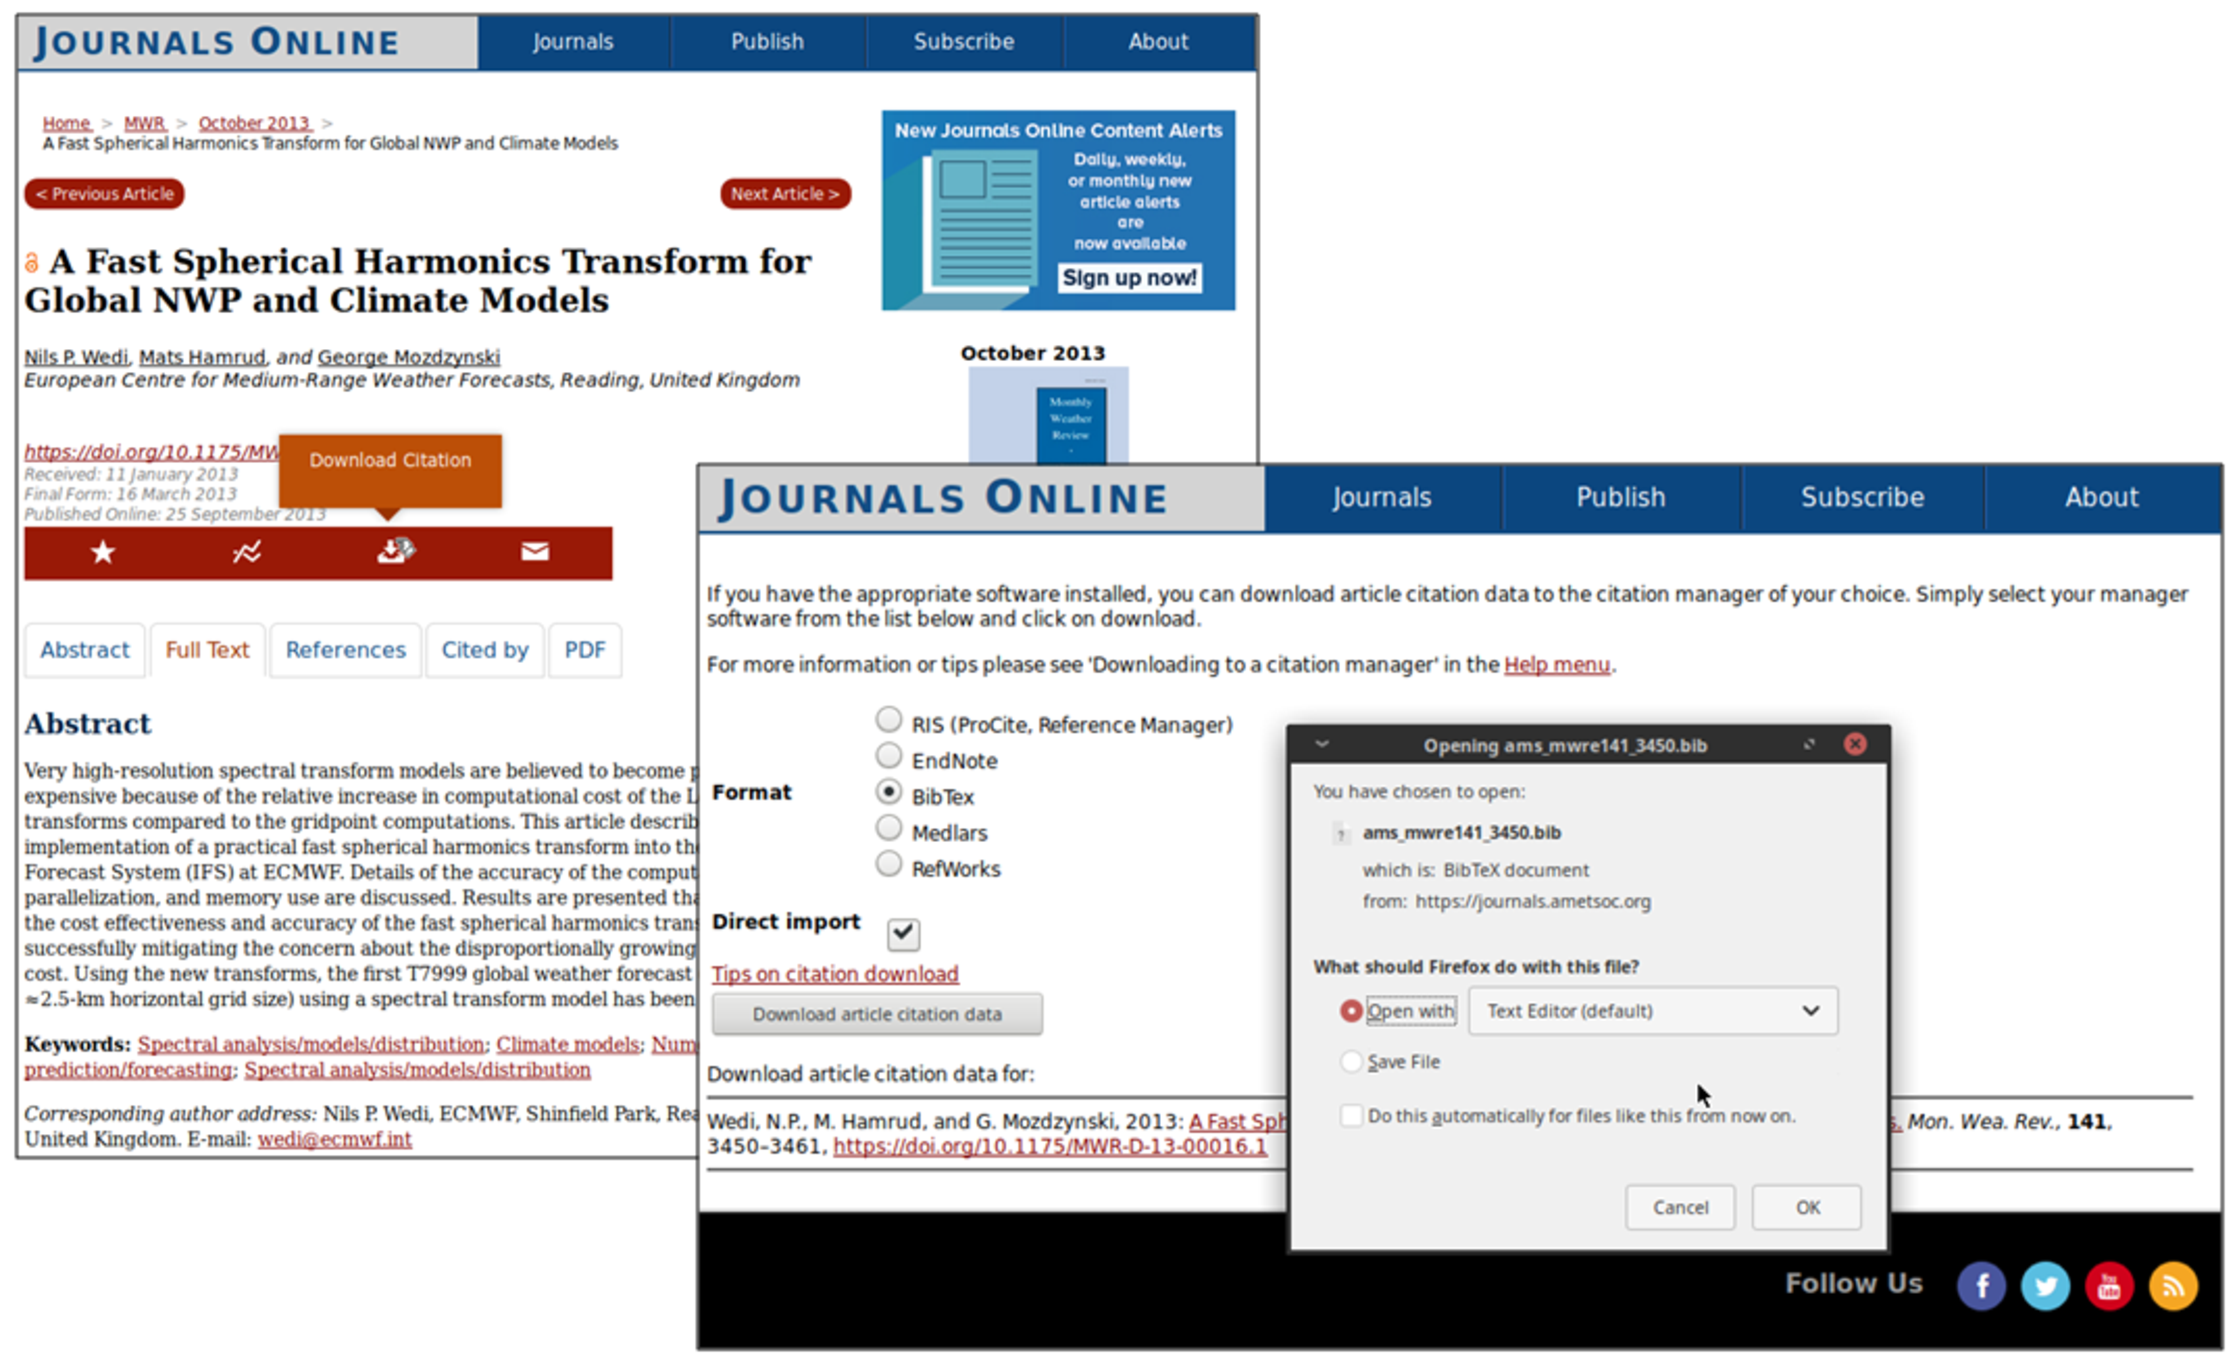
\includegraphics[scale=0.4]{./docs/figs/exemplo_revista_ams_citacao.pdf}
    \end{center}
\vspace{4mm}
\legenda{\textit{Site} da revista \textit{Monthly Weather Review}.}
\label{fig:exemplo_revista_ams_citacao}
\FONTE{Produção do autor.}
\end{figure}

No exemplo da Figura \ref{fig:exemplo_revista_ams_citacao}, o conteúdo do arquivo com a referência é mostrado a seguir:

\begin{texexp}{listing only}
@article{doi:10.1175/MWR-D-13-00016.1,
author   = {Wedi, Nils P. and Hamrud, Mats and Mozdzynski, George},
title    = {A Fast Spherical Harmonics Transform for Global NWP
            and Climate Models},
journal  = {Monthly Weather Review},
volume   = {141},
number   = {10},
pages    = {3450-3461},
year     = {2013},
doi      = {10.1175/MWR-D-13-00016.1},
URL      = {https://doi.org/10.1175/MWR-D-13-00016.1},
eprint   = {https://doi.org/10.1175/MWR-D-13-00016.1},
abstract = {Abstract Very high-resolution spectral transform models are believed to become prohibitively expensive because of the relative increase in computational cost of the Legendre transforms compared to the gridpoint computations. This article describes the implementation of a practical fast spherical harmonics transform into the Integrated Forecast System (IFS) at ECMWF. Details of the accuracy of the computations, of the parallelization, and memory use are discussed. Results are presented that demonstrate the cost effectiveness and accuracy of the fast spherical harmonics transform, successfully mitigating the concern about the disproportionally growing computational cost. Using the new transforms, the first T7999 global weather forecast (equivalent to \~2.5-km horizontal grid size) using a spectral transform model has been produced.}
}
\end{texexp}

As informações do arquivo de referência baixado, podem ser incorporadas em uma seção apropriada no documento que o usuário estiver editando. No caso do estilo do INPE, o conteúdo do arquivo pode ser copiado para dentro do arquivo {\tt bib/referencias.bib} (veja mais detalhes na Seção \ref{sec:citerefs} do Capítulo \ref{cap:parteIII}).

Observe que o arquivo de referências possui diversas palavras-chave, como por exemplo, {\tt author}, {\tt title}, {\tt journal}, {\tt volume} e outros. Estas são as informações que o Bib\TeX{} utiliza para formatar a apresentação das referências no estilo desejado.

\begin{marker}
Recomenda-se a alteração do nome da citação (a qual será usada no texto) para algo que seja mais fácil de lembrar. Isso facilitará a escrita do texto. Por exemplo, ao invés de utilizar {\tt doi:10.1175/MWR-D-13-00016.1} (como na referência do exemplo acima), utilize algo como {\tt wedietal/2013}, que faz referência literal ao artigo de \citeonline{doi:10.1175/MWR-D-13-00016.1}.
\end{marker}

A utilização das referências no texto deve ser feita com os seguintes comandos: \mintinline{latex}{\cite{referencia}} ou \mintinline{latex}{\citeonline{referencia}}. Veja o Exemplo \ref{exe:ref2} a seguir:

\begin{texexptitled}[breakable,center lower,enhanced,middle=2mm]{Exemplos de citações utilizando os comandos {\tt cite} e {\tt citeonline}}{exe:ref2}
Segundo \citeonline{wedietal/2013}, a transformada rápida de Legendre torna-se especialmente útil em modelos espectrais cujo número de onda é maior do que 2047.

A transformada rápida de Legendre torna-se especialmente útil em modelos espectrais cujo número de onda é maior do que 2047 \cite{wedietal/2013}.
\end{texexptitled}

\begin{marker}
Se você estiver utilizando o estilo de publicações específico de alguma revista científica, é possível que exista outro(s) estilo(s) de citação, como exemplo, dado pelo comando \mintinline{latex}{\citep{referencia}}.
\end{marker}

No Exemplo \ref{exe:ref2}, observe que o comando \mintinline{latex}{\cite} marca a citação com a primeira letra em caixa alta, enquanto que com o comando \mintinline{latex}{\citeonline}, a citação aparece delimitada por parênteses e com todas as letras em caixa alta. 
% REF: https://texblog.org/2012/10/22/multiple-bibliographies-with-biblatex/
%\begin{texexptitled}[breakable,center lower,enhanced,middle=2mm]{Exemplos de estilos de referências do BibTeX}{exe_estilos_bib}
%Segundo \cite{doi:10.1175/MWR-D-13-00016.1}, a transformada rápida de Legendre torna-se especialmente útil em modelos espectrais cujo número de onda seja maior do que 2047.
%
%\bibliographystyle{abbrv}
%\bibliography{./bib/referencia}
%
%\cite{doi:10.1175/MWR-D-13-00016.1} and \cite{doi:10.1175/MWR-D-13-00016.1} were published later than \citeNew{doi:10.1175/MWR-D-13-00016.1}.
%
%\bibliographystyle{plain}
%\bibliography{./bib/referencia}
%
%\bibliographystyleNew{plain}
%\bibliographyNew{./bib/referencia}
%\end{texexptitled}

% A dica a seguir foi movida para o Capítulo 3.
%\begin{marker}
%Deve-se ter cautela na edição manual do arquivo {\tt referencia.bib} do estilo do INPE. Este arquivo não aceita acentos naturais, i.e., acentos latinos devem ser marcados no estilo do \LaTeX{} (veja mais detalhes na Seção \ref{sec:acentos}. Além disso, é recomendável que o usuário edite a referência, removendo espaços em brancos e remarcando os acentos, quando necessário.
%\end{marker}

Grandes bases de referências podem ser gerenciadas com o auxílio de software como o \textit{BibDesk} (apenas para o Mac OS), \textit{JabRef}, \textit{Mendeley} e \textit{Zotero}. Estes \textit{softwares} são bastante úteis pois permitem a organização das referência e dos seus metadados e é uma boa ideia tê-las sempre organizadas. Um arquivo Bib\TeX{} (com extensão {\tt .bib}) pode ser importado para dentro destes software. Nas Figuras \ref{fig:exe_bibdesk}, \ref{fig:exe_mendeley} e \ref{fig:exe_zotero}, são mostrados como uma base de dados é carregada neste \textit{softwares}.

No \textit{BibDesk}, clique no menu ``Arquivo > Abrir...'' e selecione o arquivo {\tt .bib} com as referências. Depois de importado o arquivo, todas as referências serão mostradas em lista na janela principal. Se houver alguma referência com algum tipo de problema (e.g., caracteres não permitidos ou codificação não reconhecida), o \textit{BibDesk} irá abrir uma caixa de diálogo perguntando ao usuário se ele quer parar a importação ou continuar. Uma outra opção é revisar e editar o arquivo antes de iniciar a importação.

\begin{figure}[H]
\caption{Base de dados de referências carregada no \textit{software} \textit{BibDesk}.}
\vspace{6mm}
    \begin{center}
        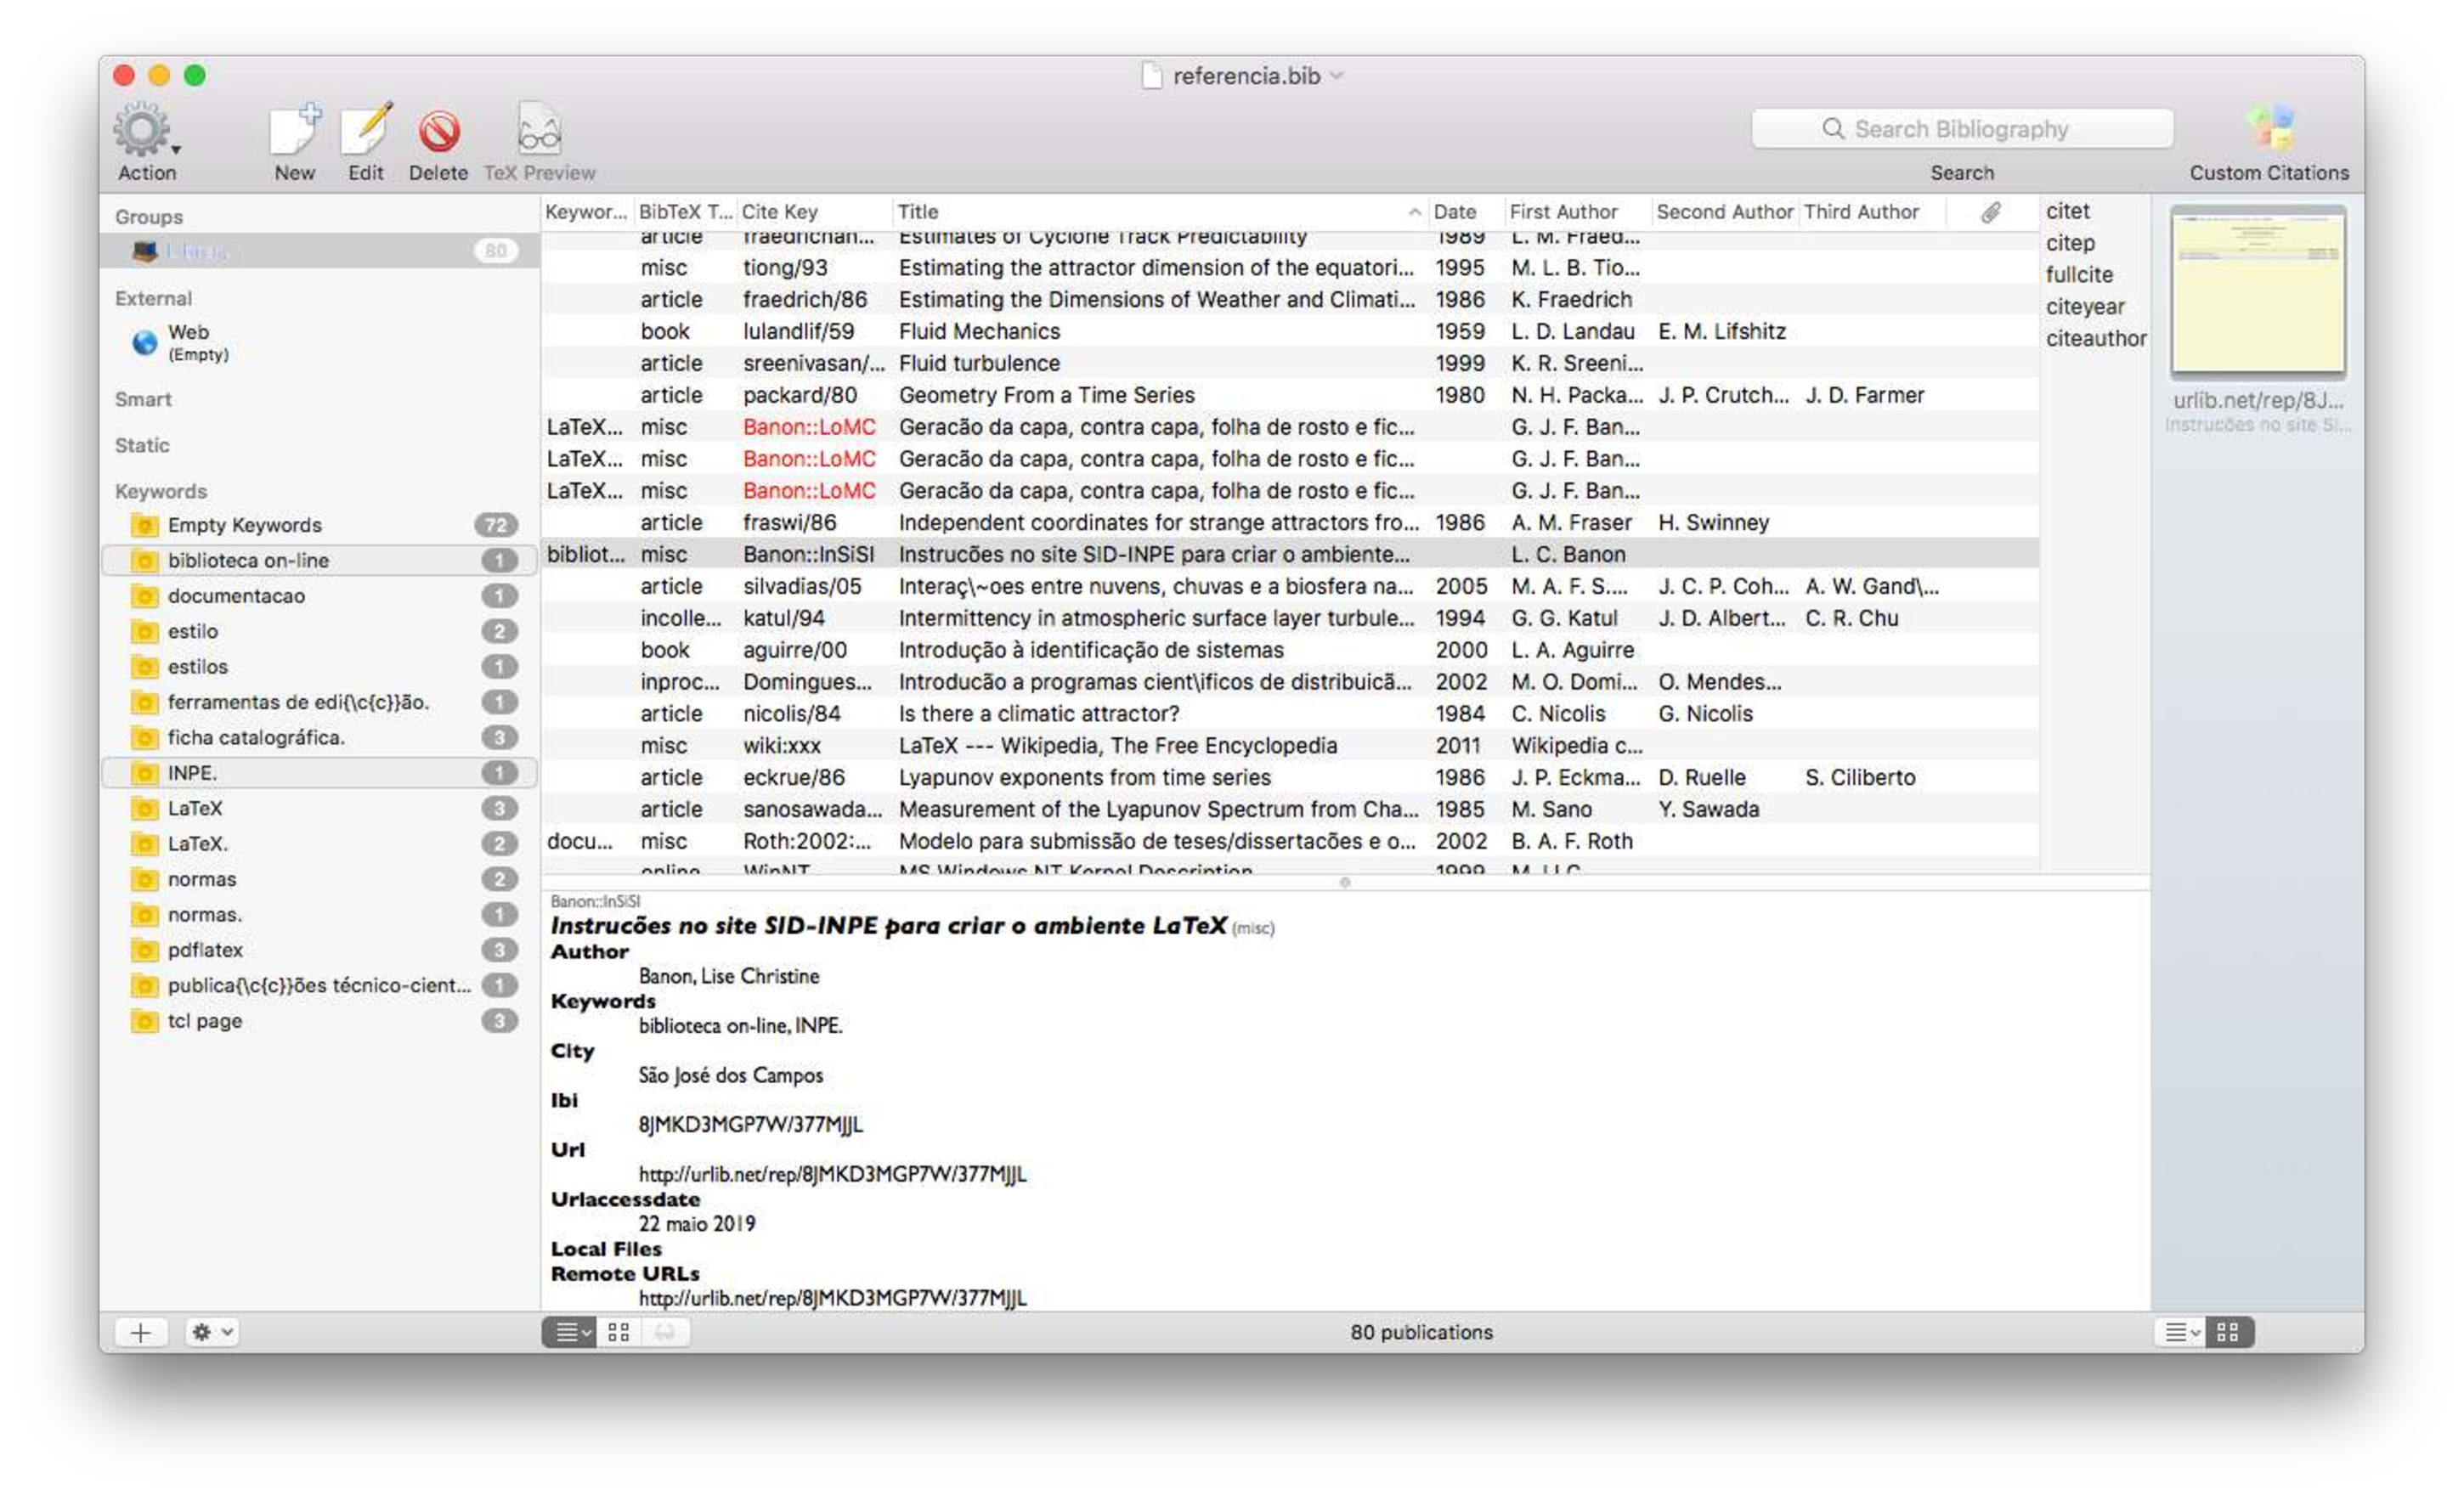
\includegraphics[scale=0.3]{./docs/figs/bibdesk.pdf}
    \end{center}
\vspace{4mm}
\legenda{\textit{Software} \textit{BibDesk}.}
\label{fig:exe_bibdesk}
\FONTE{Produção do autor.}
\end{figure}

Com o \textit{software} \textit{Mendeley}, também é possível importar um arquivo de referências {\tt .bib}, a partir do qual é possível inserir e editar entradas existentes ou então remover as entradas que não são mais necessárias. Veja a Figura \ref{fig:exe_mendeley} a seguir.
 
\begin{figure}[H]
\caption{Base de dados de referências carregada no \textit{software} \textit{Mendeley}.}
\vspace{6mm}
    \begin{center}
        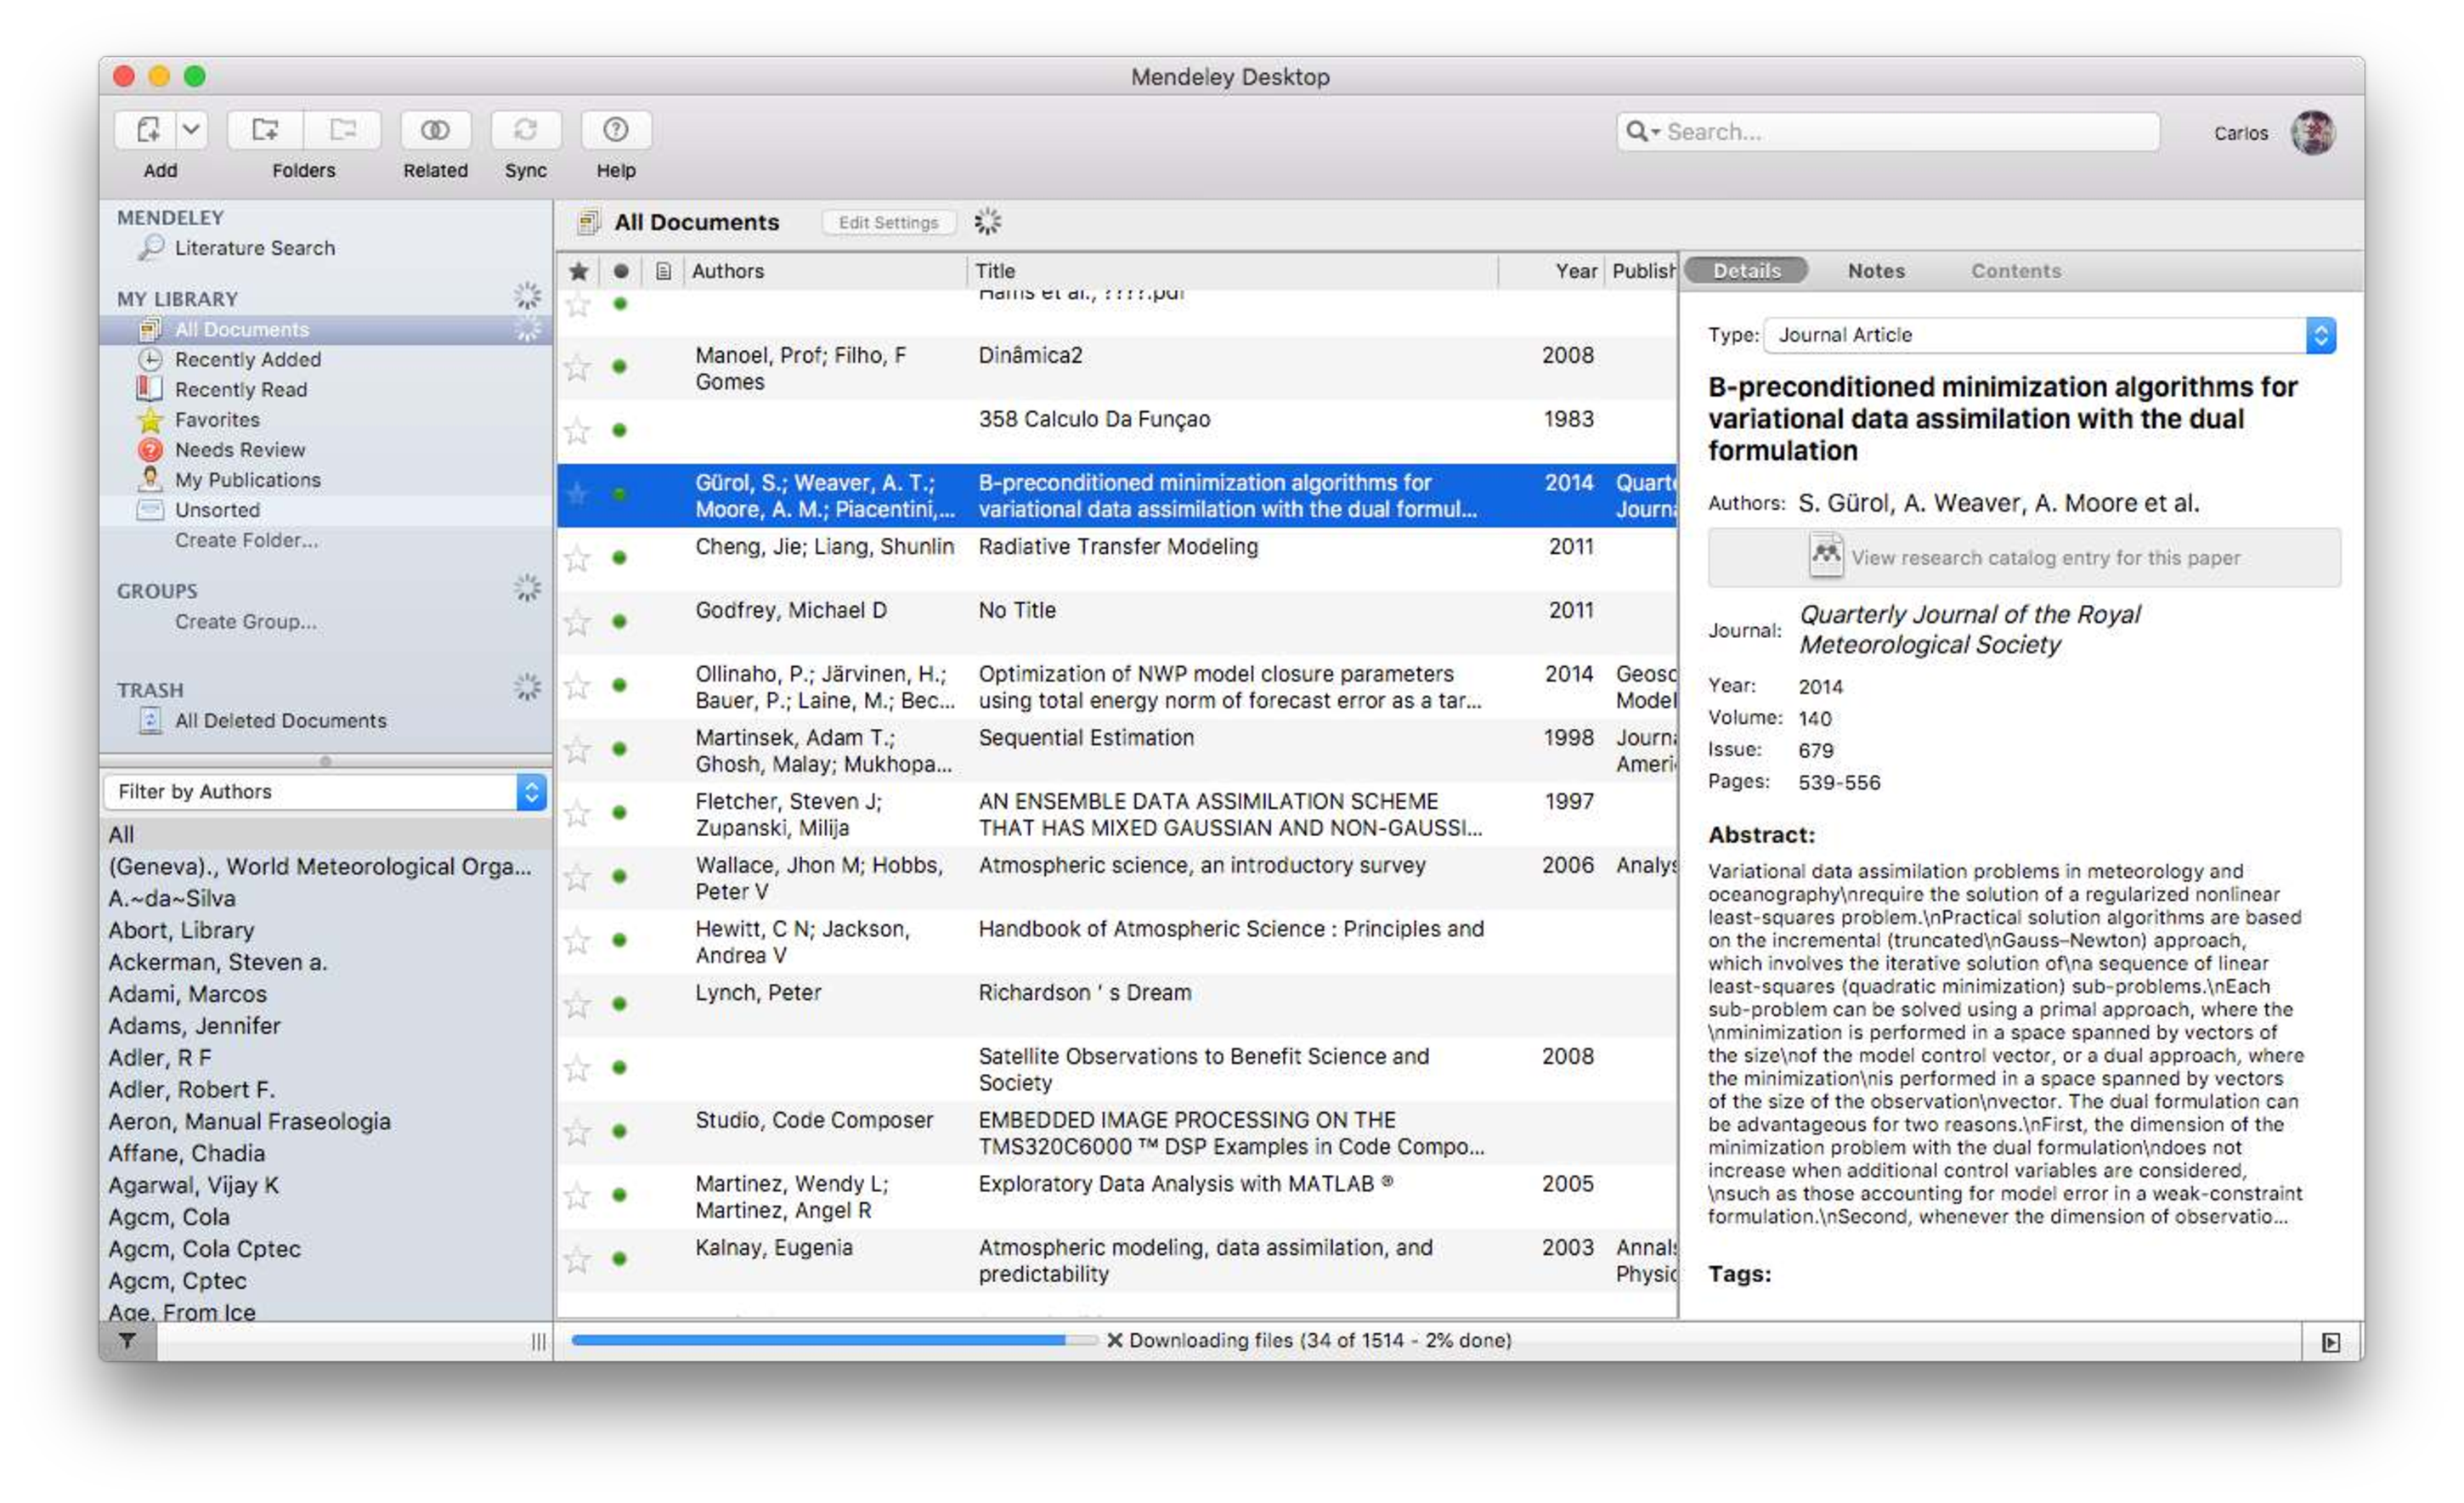
\includegraphics[scale=0.3]{./docs/figs/mendeley.pdf}
    \end{center}
\vspace{4mm}
\legenda{\textit{Software} \textit{Mendeley}.}
\label{fig:exe_mendeley}
\FONTE{Produção do autor.}
\end{figure}

Análogo aos \textit{softwares} \textit{BibDesk} e \textit{Mendeley}, pode-se também utilizar o \textit{software} \textit{Zotero} para a mesma finalidade (Figura \ref{fig:exe_zotero}). Note que com excessão do \textit{software} \textit{BibDesk}, os \textit{softwares} \textit{Mendeley} e \textit{Zotero} estão disponíveis para os sistemas operacionais Linux e \textit{Microsoft Windows}.

\begin{figure}[H]
\caption{Base de dados de referências carregada no \textit{software} \textit{Zotero}.}
\vspace{6mm}
    \begin{center}
        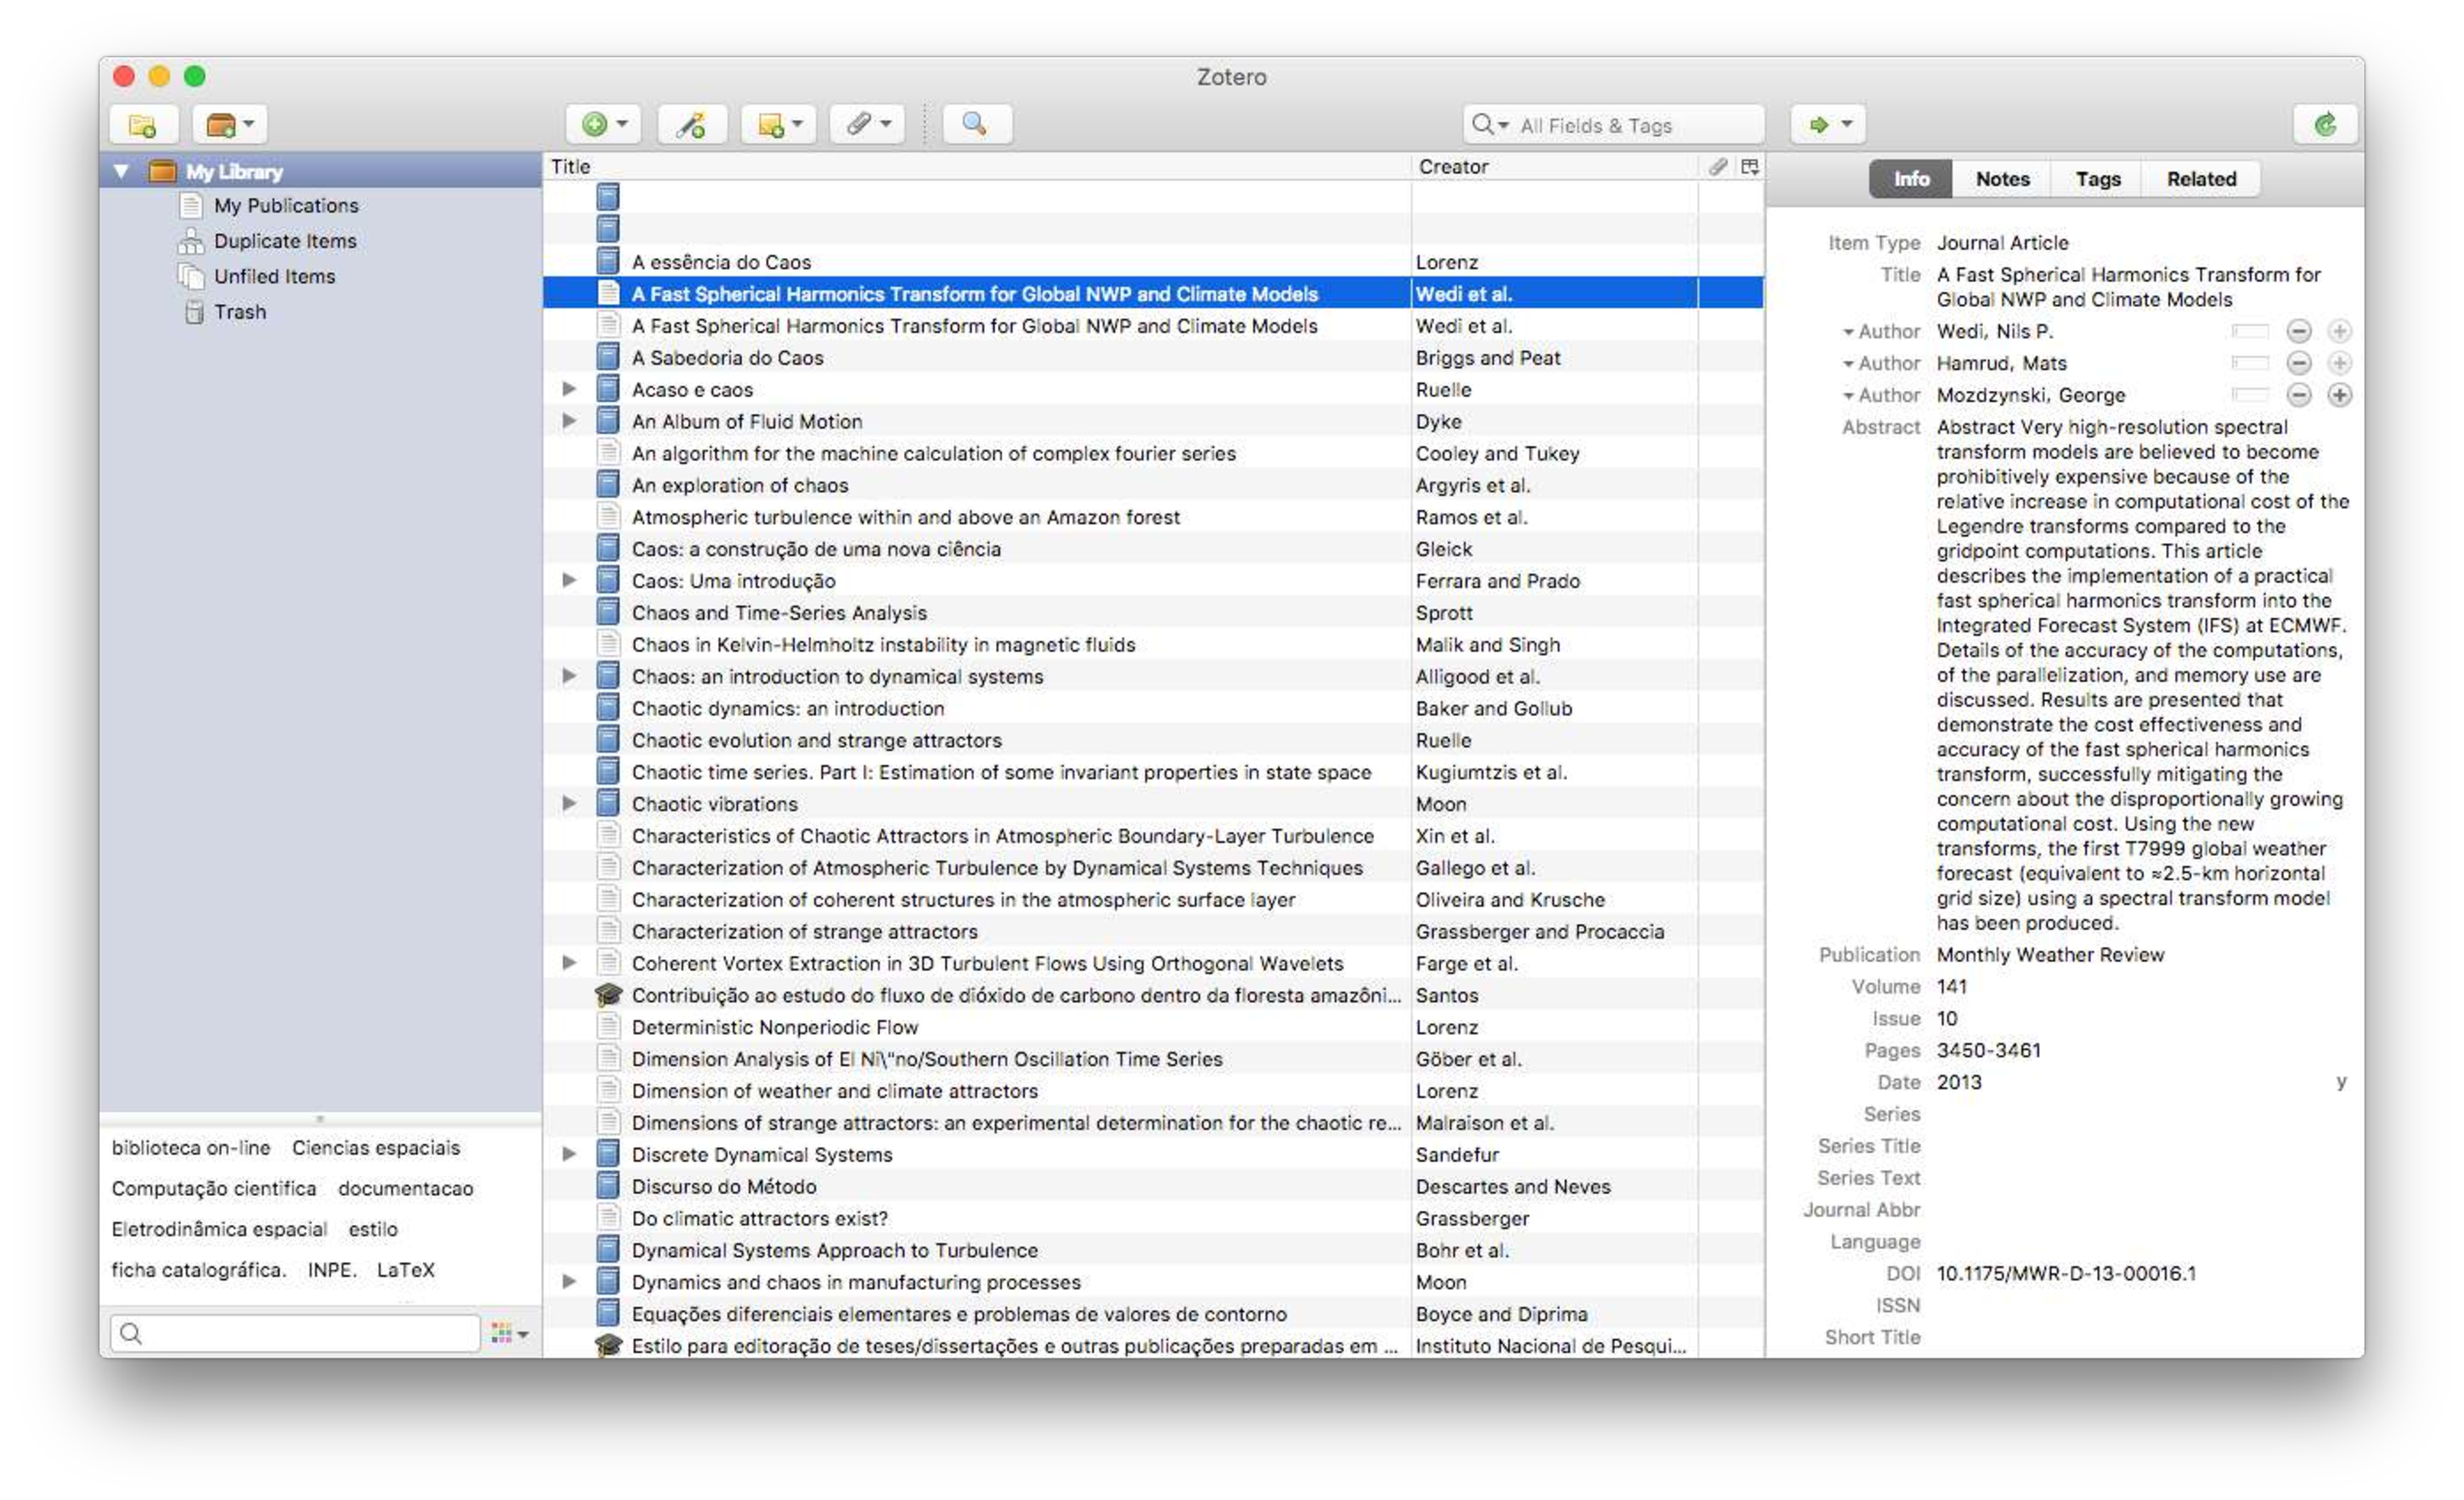
\includegraphics[scale=0.3]{./docs/figs/zotero.pdf}
    \end{center}
\vspace{4mm}
\legenda{\textit{Software} \textit{Zotero}.}
\label{fig:exe_zotero}
\FONTE{Produção do autor.}
\end{figure}

\subsubsection*{Tipos de Referências}
\label{sec:estilos_refs}

O Bib\TeX{} possui diversos tipos de referências, os quais devem ser adequadamente utilizados a fim de que sejam mostradas as informações corretas para cada citação que se fizer no texto.

A Tabela \ref{tab:refs} a seguir descreve os tipos de referências padrão do Bib\TeX{}.

\begin{table}[H]
\centering
\caption{Tipos de referências padrão do Bib\TeX{}.}
\label{tab:refs}
    \begin{tabular}{p{4cm}p{9cm}}
    \toprule
    \textbf{Tipo} & \textbf{Descrição} \\
    \midrule
    {\tt article}       & Artigo de jornal ou revista \\
    {\tt book}          & Livro publicado \\
    {\tt booklet}       & Compilação de trabalhos em formato de livro com vários autores, mas sem editora ou patrocinador \\
    {\tt inbook}        & Parte ou capítulo de um livro, sem o título do livro ao qual pertence \\
    {\tt incollection}  & Parte ou capítulo de um livro, com o título do livro ao qual pertence \\
    {\tt inproceedings} & Artigo em anais de congresso ou conferência \\
    {\tt conference}    & Idem a {\tt inproceedings} \\
    {\tt manual}        & Manual técnico \\
    {\tt masterthesis}  & Dissertação de mestrado \\
    {\tt phdthesis}     & Tese de doutorado \\
    {\tt misc}          & Modelo útil para outros tipos de referências \\
    {\tt proceedings}   & Anais de congresso ou conferência \\
    {\tt techreport}    & Relatório técnico \\
    {\tt unpublished}   & Artigo, livro ou outro tipo de trabalho não publicado \\
    \bottomrule
    \end{tabular}
\FONTE{Produção do autor.}
\end{table}

\begin{marker}
Os tipos de referências descritos na Tabela \ref{tab:refs} possuem campos que são obrigatórios e outros que são opcionais. Veja mais detalhes sobre os campos obrigatórios de cada tipo em \url{https://en.wikibooks.org/wiki/LaTeX/Bibliography_Management}.
\end{marker}

No \textit{site} da biblioteca do INPE, todas as referências já se encontram classificadas no tipo correto. Para obtê-las, basta procurar pelo trabalho no \textit{site} e clicar no link ``Bib\TeX{}''. O arquivo aberto na janela \textit{popup} poderá ser copiado para o arquivo de refrências do Bib\TeX{} (arquivo com extensão {\tt .bib}). Veja um exemplo na Figura \ref{fig:bibliotex} a seguir.

\begin{figure}[H]
\caption{Obtenção de referências no formato Bib\TeX{} a partir do \textit{site} da biblioteca do INPE.}
\vspace{6mm}
    \begin{center}
        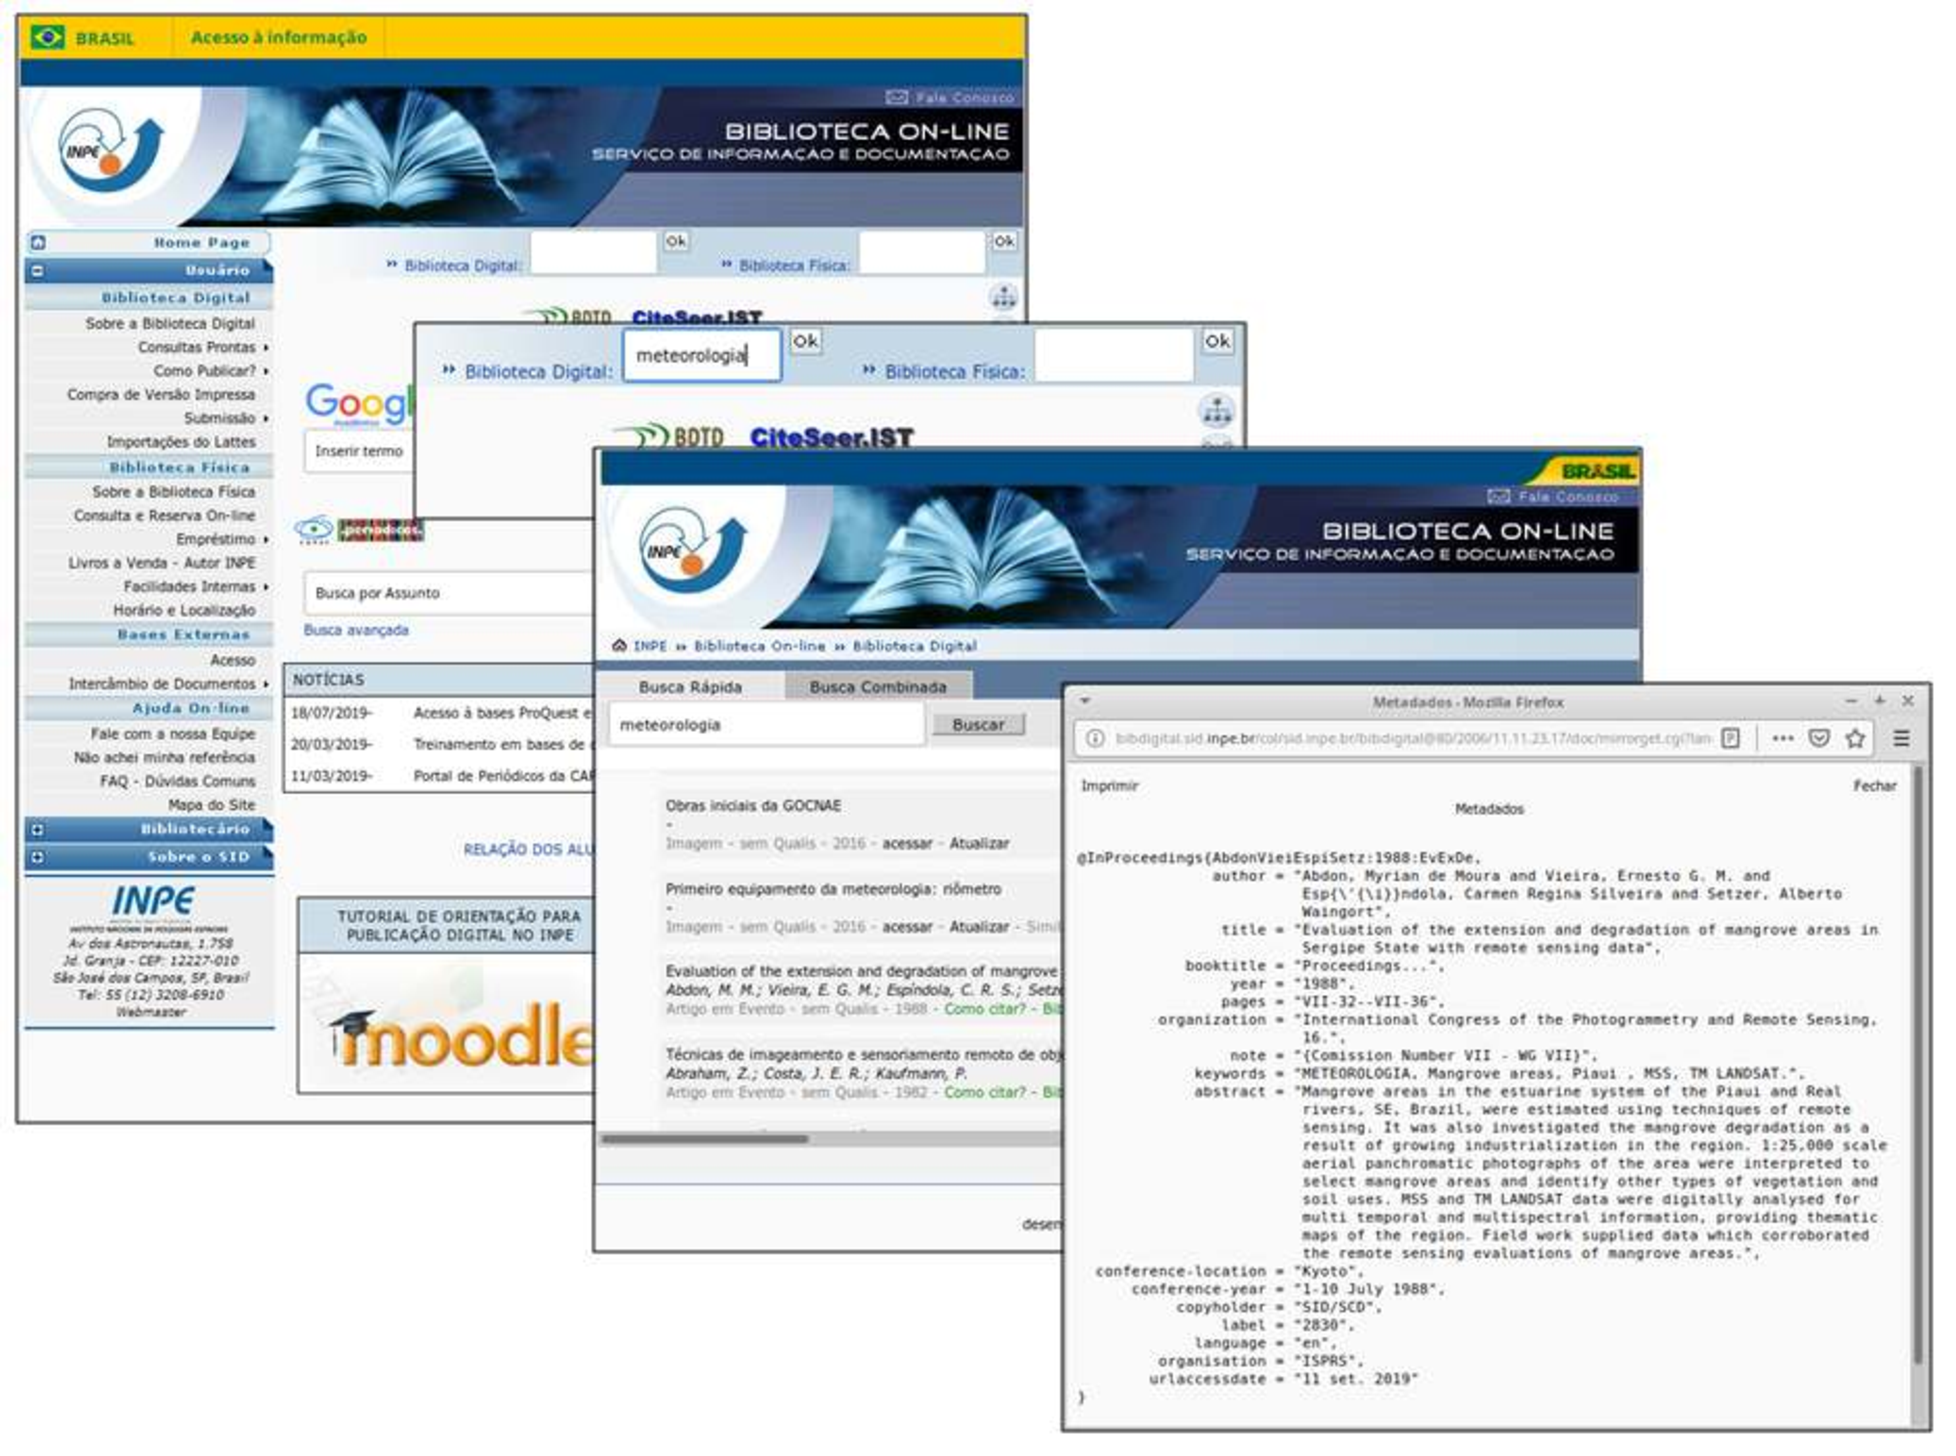
\includegraphics[scale=0.45]{./docs/figs/bibliotex.pdf}
    \end{center}
\vspace{4mm}
\legenda{Site da biblioteca do INPE.}
\label{fig:bibliotex}
\FONTE{Produção do autor.}
\end{figure}

%É possível utilizar diferentes estilos de referências. No estilo do INPE, utiliza-se o modelo da Associação Brasileira de Normas Técnicas (ABNT), que é provido a partir da utilização do pacote {\tt abntex2} (carregado automaticamente com o estilo do INPE). Em um documento livre, o usuário pode escolher outros estilos. Para isto, basta utilizar o comando \mintinline{latex}{\bibliographystyle}, indicando-se o estilo como argumento do marcador.

\begin{marker}
Se uma referência de um trabalho no formato Bib\TeX{} não puder ser encontrada nos \textit{sites} das revistas indexadas, pode-se utilizar o serviço do \textit{site} \href{https://doi2bib.org}{\textit{DOI2Bib}} para se obter a referência com os campos corretos.
\end{marker}

%\subsubsection*{Referências cruzadas}
%\label{sec:refs_cruz}

%\subsubsection*{Índice remissivo}
%\label{sec:ind_rem}

%\subsubsection*{Glossário}
%\label{sec:glossario}
%http://linorg.usp.br/CTAN/macros/latex/contrib/glossaries/glossaries-user.html#sec:lipsum

\subsection{\textit{Macros}}
\label{sec:macros}

No \LaTeX{} é possível definir \textit{macros}, que são um conjunto de instruções específicas que visam facilitar a formatação do documento. Além das \textit{macros}, é possível também redefinir comandos do \LaTeX{}, de forma que os comandos originais sejam executados de forma mais simples e customizada.

O livro de \citeonline{knuth/1996} oferece uma introdução concisa sobre a linguagem \textit{macro} do \LaTeX{}. O leitor já deve ter percebido que todas as ocorrências da palavra ``LaTeX'' são mostradas na forma estilizada \LaTeX{}. Isto é feito através da uma \textit{macro} que é definida pelo comando \mintinline{latex}{\LaTeX{}}, que então produz a grafia estilizada da palavra. Esta \textit{macro} define não apenas o estilo da fonte utilizada, mas também os espaçamentos horizontal e vertical. Aliás, todos os comandos da linguagem que já foram mostrados, são definidos por \textit{macros}. Logo, pode-se entender que as \textit{macros} constituem um conjunto de instruções que permitem manipular a linguagem de forma que determinadas ações sejam feitas sem a necessidade de programá-las sempre que for necessário reutilizá-las. Apesar disso, \textit{macros} são diferentes de \textit{scripts}, pois \textit{scripts} são códigos independentes que são interpretados e executados linha-a-linha. No \LaTeX{}, as \textit{macros} são incluídas no preâmbulo documentos e são utilizadas para estruturar o documento.

O leitor perceberá a importância das \textit{macros} quando precisar fazer uso de alguma configuração mais do que uma vez. Um exemplo bastante simples, é definir um comando (que nada mais é do que uma \textit{macro}) para inserir uma informação que pode ser repetida em diferentes partes do texto. Suponha que queiramos que a expressão ``por exemplo'' seja inserida sempre que digitarmos o comando \mintinline{latex}{\eg} e que a expressão ``isto é'' seja inserida sempre que digitar o comando \mintinline{latex}{\ie}. No \LaTeX{} os comandos \mintinline{latex}{\eg} e \mintinline{latex}{\ie} não existem, então podemos utilizá-los para este propósito. Veja no Exemplo \ref{exe_macro0} como fazer isso.

\begin{texexptitled}[breakable,center lower,enhanced,middle=2mm]{Definindo um comando simples de substituição}{exe_macro0}
\newcommand{\eg}{por exemplo}
\newcommand{\ie}{isto é}

Documentos \LaTeX{}, independente da sua classe (\eg, \textit{book}, 
\textit{report}, \textit{article} e \textit{letter}), podem ser muito simples ou complexos.

\dots

Entretanto, em algumas situações é necessário marcar os acentos de forma explícita (\eg, na edição de um arquivo de referências do BibTeX). 

\dots

No Exemplo \ref{exe_eq0}, observe que os delimitadores dados por colchetes ou parênteses precisar ser ``escapados'', \ie, é necessário adicionar uma \verb|\| (barra invertida) antes deles (\eg, \verb|\[| e \verb|\]| ou \verb|\(| e \verb|\)|). 
\end{texexptitled}

\begin{marker}
No Exemplo \ref{exe_macro0}, observe ainda que o comando \mintinline{latex}{\dots} é também uma \textit{macro} que produz as reticências (\dots).
\end{marker}

Considere os Exemplos \ref{exe_tab2} e \ref{exe_tab3} em que o espaçamento \mintinline{latex}{\\[-0.5em]} é utilizado múltiplas vezes para definir a altura das linhas das tabelas mostradas. Este comando pode ser ``empacotado'' através da definição de uma \textit{macro} que simplesmente irá abreviar o seu uso, no sentido de torná-lo mais simples. Para isto, veja o Exemplo \ref{exe_macro1} a seguir.

\begin{texexptitled}[breakable,center lower,enhanced,middle=2mm,listing side text]{Definindo um simples comando de espaçamento}{exe_macro1}
\newcommand{\recuo}{\\[-0.5em]}

\begin{tabular}{l r}
\hline 
\recuo
\textbf{L0C1} & \textbf{L0C2} \\
\recuo
\hline
\recuo
L1C1 & L1C2 \\
\recuo
L2C1 & L2C2 \\
\recuo
L3C1 & L3C2 \\
\recuo
L4C1 & L4C2 \\
\recuo
L5C1 & L5C2 \\
\recuo
\hline
\end{tabular}
\end{texexptitled}

Muitas vezes será necessário incluir um espaço em branco extra, o que pode ser obtido incluindo-se um par de \verb|{}|'s (chaves) após o comando, e.g., como em \mintinline{latex}{\LaTeX{}} ou \mintinline{latex}{\LaTeX}, que irá produzir \LaTeX{} e \LaTeX, respectivamente. Considere os comandos {\tt inpe} e {\tt inpee} do Exemplo \ref{exe_macro2} a seguir e compare os resultados das suas aplicações, com e sem as \verb|{}|'s: 

\begin{texexptitled}[breakable,center lower,enhanced jigsaw,middle=2mm]{Definindo um comando simples de substituição com espaço extra}{exe_macro2}
\newcommand{\inpe}{INPE}
\newcommand{\inpee}{INPE }

\begin{enumerate}
  \item O \inpe desenvolve pesquisas relacionadas às ciências atmosféricas e espaciais.
  \item Pesquisas relacionadas às ciências atmosféricas e espaciais são desenvolvidas no \inpe.
  \item O \inpe{} desenvolve pesquisas relacionadas às ciências atmosféricas e espaciais.
  \item Pesquisas relacionadas às ciências atmosféricas e espaciais são desenvolvidas no \inpe{}.
  \item O \inpee desenvolve pesquisas relacionadas às ciências atmosféricas e espaciais.
  \item Pesquisas relacionadas às ciências atmosféricas e espaciais são desenvolvidas no \inpee.
  \item O \inpee{} desenvolve pesquisas relacionadas às ciências atmosféricas e espaciais.
  \item Pesquisas relacionadas às ciências atmosféricas e espaciais são desenvolvidas no \inpee{}.
\end{enumerate}
\end{texexptitled}

No Exemplo \ref{exe_macro2} foram definidas macros que substituem a palavra-chave {\tt inpe} (ou {\tt inpee}) por INPE. Quando uma \textit{macro} é definida e utilizada em diversas partes de um documento, a sua substituição por um outro valor pode ser rápida e facilmente realizada através do comando \mintinline{latex}{\renewcommand}. Veja o Exemplo \ref{exe_macro3} a seguir:

\begin{texexptitled}[breakable,center lower,enhanced,middle=2mm]{Redefinindo um comando simples}{exe_macro3}
\renewcommand{\inpe}{Instituto Nacional de Pesquisas Espaciais}

O \inpe{} desenvolve pesquisas relacionadas às ciências atmosféricas e espaciais.

Pesquisas relacionadas às ciências atmosféricas e espaciais são desenvolvidas no \inpe{}.
\end{texexptitled}

A definição de \textit{macros} a partir do comando \mintinline{latex}{\newcommand{}{}} aceita a utilização de parâmetros (ou argumentos), tal como um \textit{script}. Veja o Exemplo \ref{exe_macro4} a seguir:

\begin{texexptitled}[breakable,center lower,enhanced,middle=2mm]{Passando parâmetros para \textit{macros}}{exe_macro4}
\newcommand{\meusomatorio}[3]{\ensuremath{\sum_{#1}^{#2}{#3}}}

O somatório de todos os números naturais pode ser expresso por: 
\meusomatorio{i=1}{\infty}{i}, $\forall i \in \mathbb{N^*}$.
\end{texexptitled}

No Exemplo \ref{exe_macro4}, observe que utilizou-se o comando \mintinline{latex}{\newcommand{}[]{}} para se definir uma expressão para a soma de todos os números naturais não nulos. Neste caso, \verb|{\meusomatorio}| define o nome do comando, \verb|[3]| indica a quantidade de argumentos que este novo comando deverá receber e \verb|{\ensuremath{\sum_{#1}^{#2}{#3}}}| indica a expressão matemática a ser utilizada, i.e., $\sum$ sendo que os valores indicados por \verb|#1|, \verb|#2| e \verb|#3|, são os argumentos a serem inseridos na expressão e na ordem em que devem ser informados. Além disso, observe também que a expressão definida pelo comando, é precedida pela \textit{macro} \mintinline{latex}{\ensuremath{}}, que tem a função de definir o ambiente de matemática para a expressão. Finalmente, o novo comando (\mintinline{latex}{\meusomatorio{}{}{}}) pode ser utilizado em linha sem a necessidade de se utilizar delimitadores (como indicado no início da Seção \ref{sec:mat_eqs}).

\begin{marker}
Para conhecer mais sobre a utilização de \textit{macros} para a definição de comandos e ambientes, veja em \url{https://www.overleaf.com/learn/latex/Defining_your_own_commands}.
\end{marker}

% Exemplo: redefinir o comando arraystretch de forma que a distância entre as linhas seja sempre um pouco maior (em comparação com o original): \renewcommand{\arraystretch}{1.2}

\subsection{Editores}
\label{sec:editores}

Muitos editores podem ser utilizados para editar documentos \LaTeX{}. A escolha de um editor é particular, mas pode ser associada à forma como o usuário está mais habituado a digitar. Por exemplo, se o usuário gosta de utilizar o editor \href{https://www.vim.org}{VIM} (disponível para os sistemas operacionais Linux, \textit{Microsoft Windows} e Mac OS), pode escolher instalar algumas extensões para este editor, a fim de torná-lo mais eficiente para a edição de documentos \LaTeX{}. Editores locais podem variar de acordo com o sistema operacional em uso, embora muitos projetos \textit{open source} forneçam executáveis para os sistemas operacionais mais utilizados. Em relação aos editores \textit{online}, estes podem ser mais vantajosos por não dependerem do tipo de sistema operacional, mas apenas de uma conexão com a internet e um navegador compatível. Outra vantagem dos editores \textit{online}, é o fato de que estes podem ser integrados a outros serviços, como o \href{https://dropbox.com}{Dropbox} ou o \href{https://github.com}{GitHub}.

Nas duas seções a seguir, são apresentados alguns editores selecionados para a edição de documentos \LaTeX{}.

\subsubsection*{Editores locais}
\label{sec:ed_local}

Para compilar um documento \LaTeX{} localmente, dependendo do sistema operacional em uso, há várias opções de editores. Por simplicidade, sugere-se o editor \Tex\textit{Studio}, disponível para os sistemas operacional Linux, \textit{Microsoft Windows}, e Mac OS. A Figura \ref{fig:editortexstudio} a seguir mostra o aspecto do editor \TeX\textit{Studio}.

\begin{figure}[H]
\caption{O Editor \TeX\textit{Studio}.}
\vspace{6mm}
  \begin{center}
    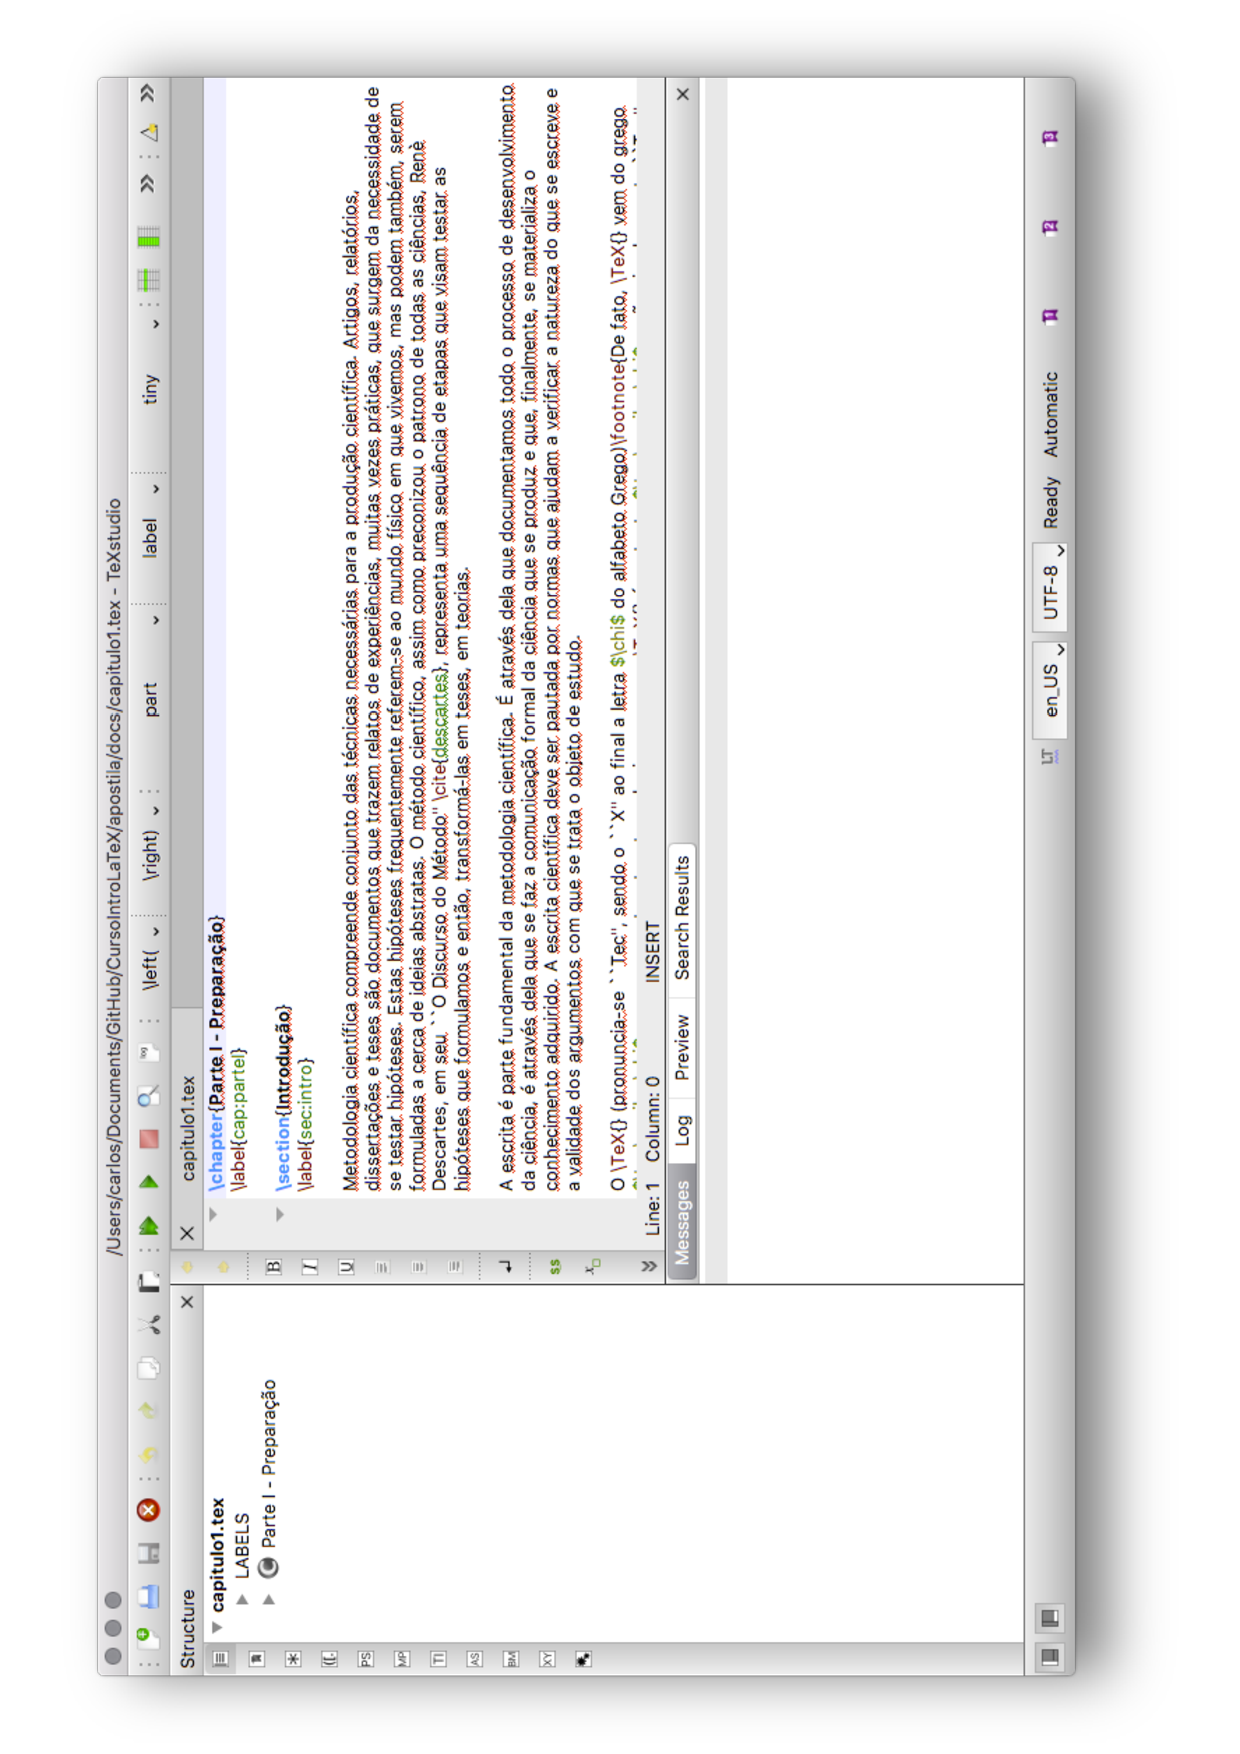
\includegraphics[width=0.7\textwidth,angle=-90]{./docs/figs/texstudio.pdf}
  \end{center}
\vspace{4mm}
\legenda{Edição local de um documento \LaTeX{} com o editor \TeX\textit{Studio}.}
\label{fig:editortexstudio}
\FONTE{Produção do autor.}
\end{figure}

Se a escolha do usuário for a linha de comando, utilizando um editor como o VIM, os documentos em \LaTeX{} podem ser compilados utilizando a sequência de comandos apresentada na Seção \ref{sec:intro_latex}. Veja na Figura \ref{fig:editorvim} um exemplo do aspecto da edição de um documento \LaTeX{} utilizando o VIM.

\begin{figure}[H]
\caption{O editor VIM (modo texto).}
\vspace{6mm}
  \begin{center}
    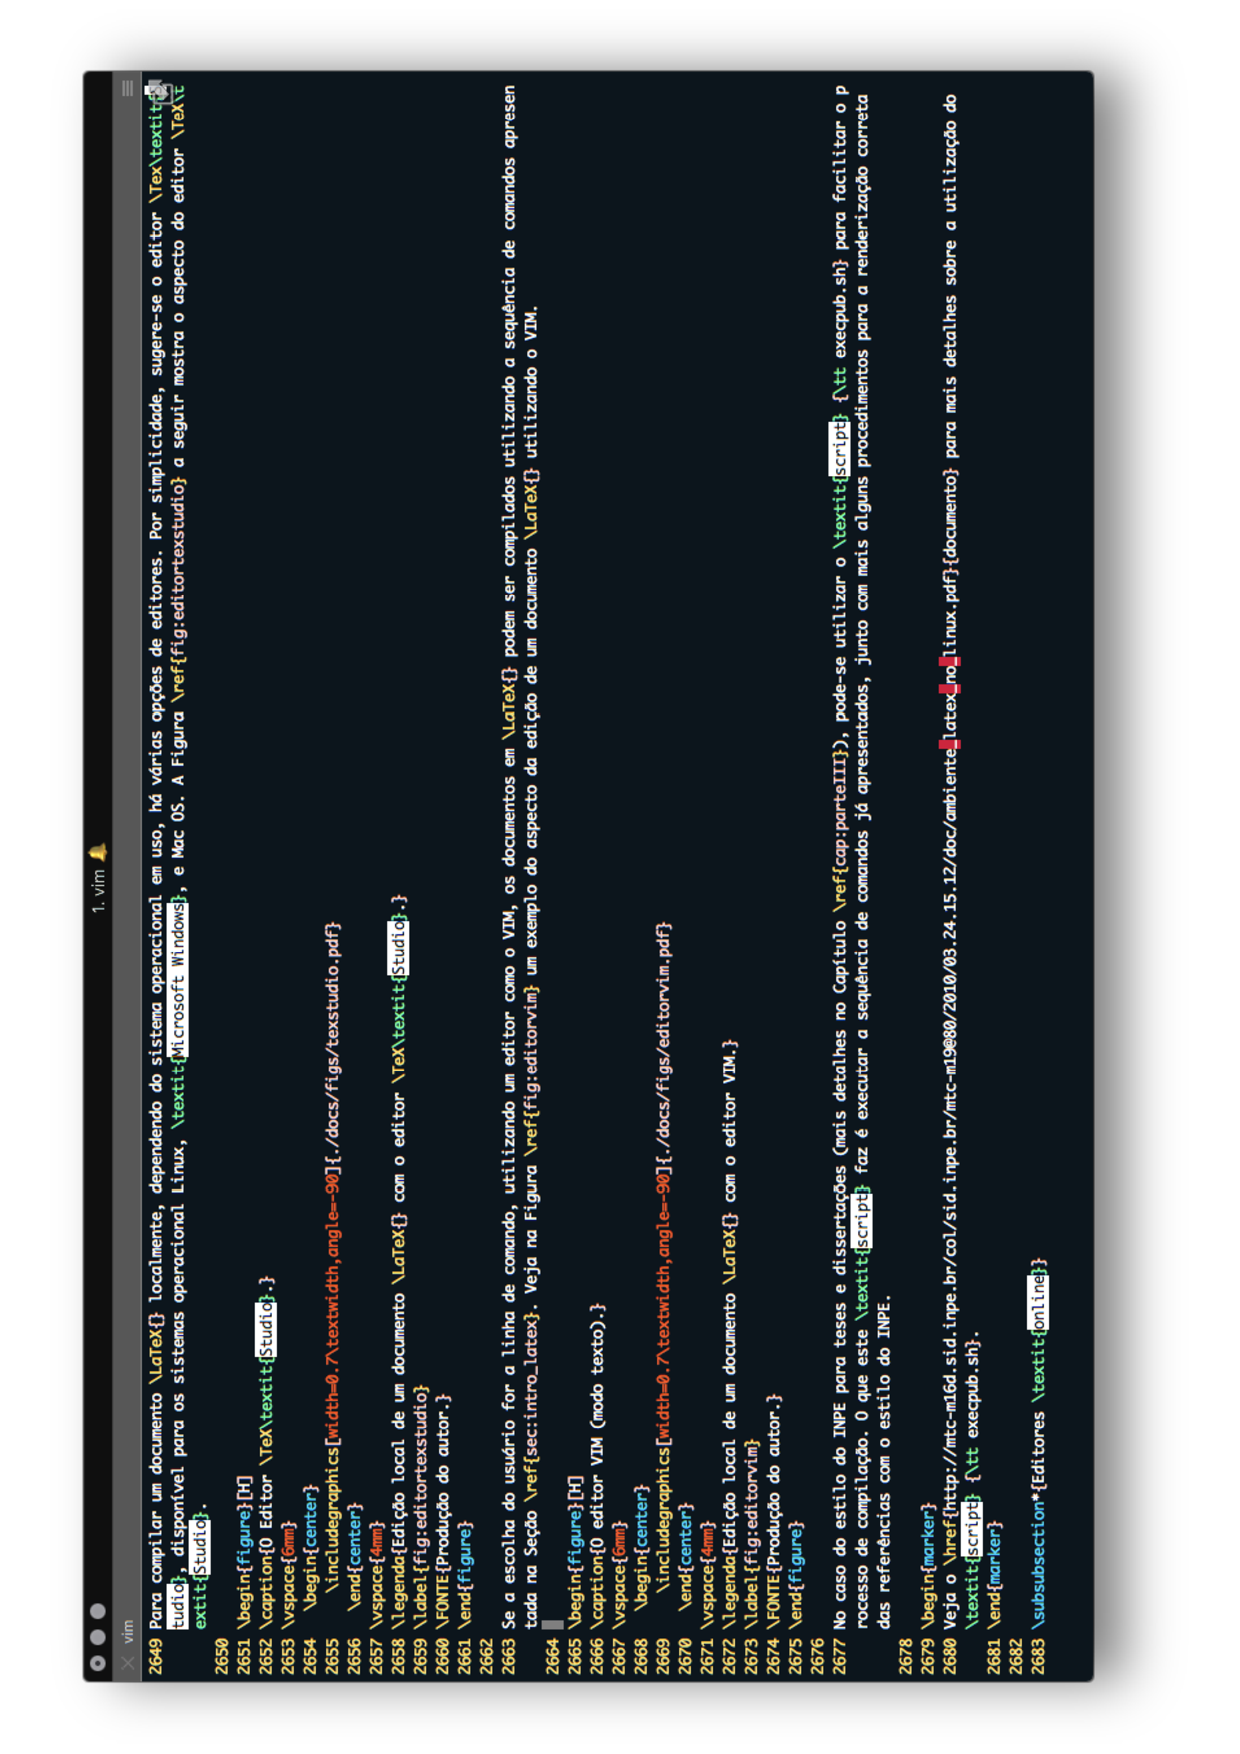
\includegraphics[width=0.7\textwidth,angle=-90]{./docs/figs/editorvim.pdf}
  \end{center}
\vspace{4mm}
\legenda{Edição local de um documento \LaTeX{} com o editor VIM.}
\label{fig:editorvim}
\FONTE{Produção do autor.}
\end{figure}

No caso do estilo do INPE para teses e dissertações (mais detalhes no Capítulo \ref{cap:parteIII}), pode-se utilizar o \textit{script} {\tt execpub.sh} para facilitar o processo de compilação. O que este \textit{script} faz é executar a sequência de comandos já apresentados, junto com mais alguns procedimentos para a renderização correta das referências com o estilo do INPE. 

\begin{marker}
Veja o \href{http://mtc-m16d.sid.inpe.br/col/sid.inpe.br/mtc-m19@80/2010/03.24.15.12/doc/ambiente_latex_no_linux.pdf}{documento} para mais detalhes sobre a utilização do \textit{script} {\tt execpub.sh}.
\end{marker}

\subsubsection*{Editores \textit{online}}
\label{sec:ed_online}

O \textit{Overleaf} é um editor \LaTeX{} \textit{online} que pode ser utilizado para escrita colaborativa. O estilo do INPE está disponível na plataforma \textit{online} e pode ser carregado para a escrita de teses e dissertações a partir de endereço \url{https://www.overleaf.com/latex/templates/inpe-thesis-template/scdyfqzhbycc#.Wrj8gH8h2Uk}. Para acessar, é necessário que o usuário crie uma conta para o acesso. Esta é a forma recomendada para a criação de documentos \LaTeX{}, especialmente se o usuário ainda não está familiarizado com documentos mais complexos como o estilo do INPE. 

O estilo para teses e dissertações do INPE pode ser aberto para edição \textit{online} com o editor \textit{Overleaf}. Para isso, acesso o \textit{link} \url{https://www.overleaf.com/latex/templates/inpe-thesis-template/scdyfqzhbycc} e abra o estilo como um template para a edição, assim como mostrado na Figura \ref{fig:overleaf1}.

\begin{figure}[H]
\caption{O editor \textit{Overleaf}.}
\vspace{6mm}
  \begin{center}
    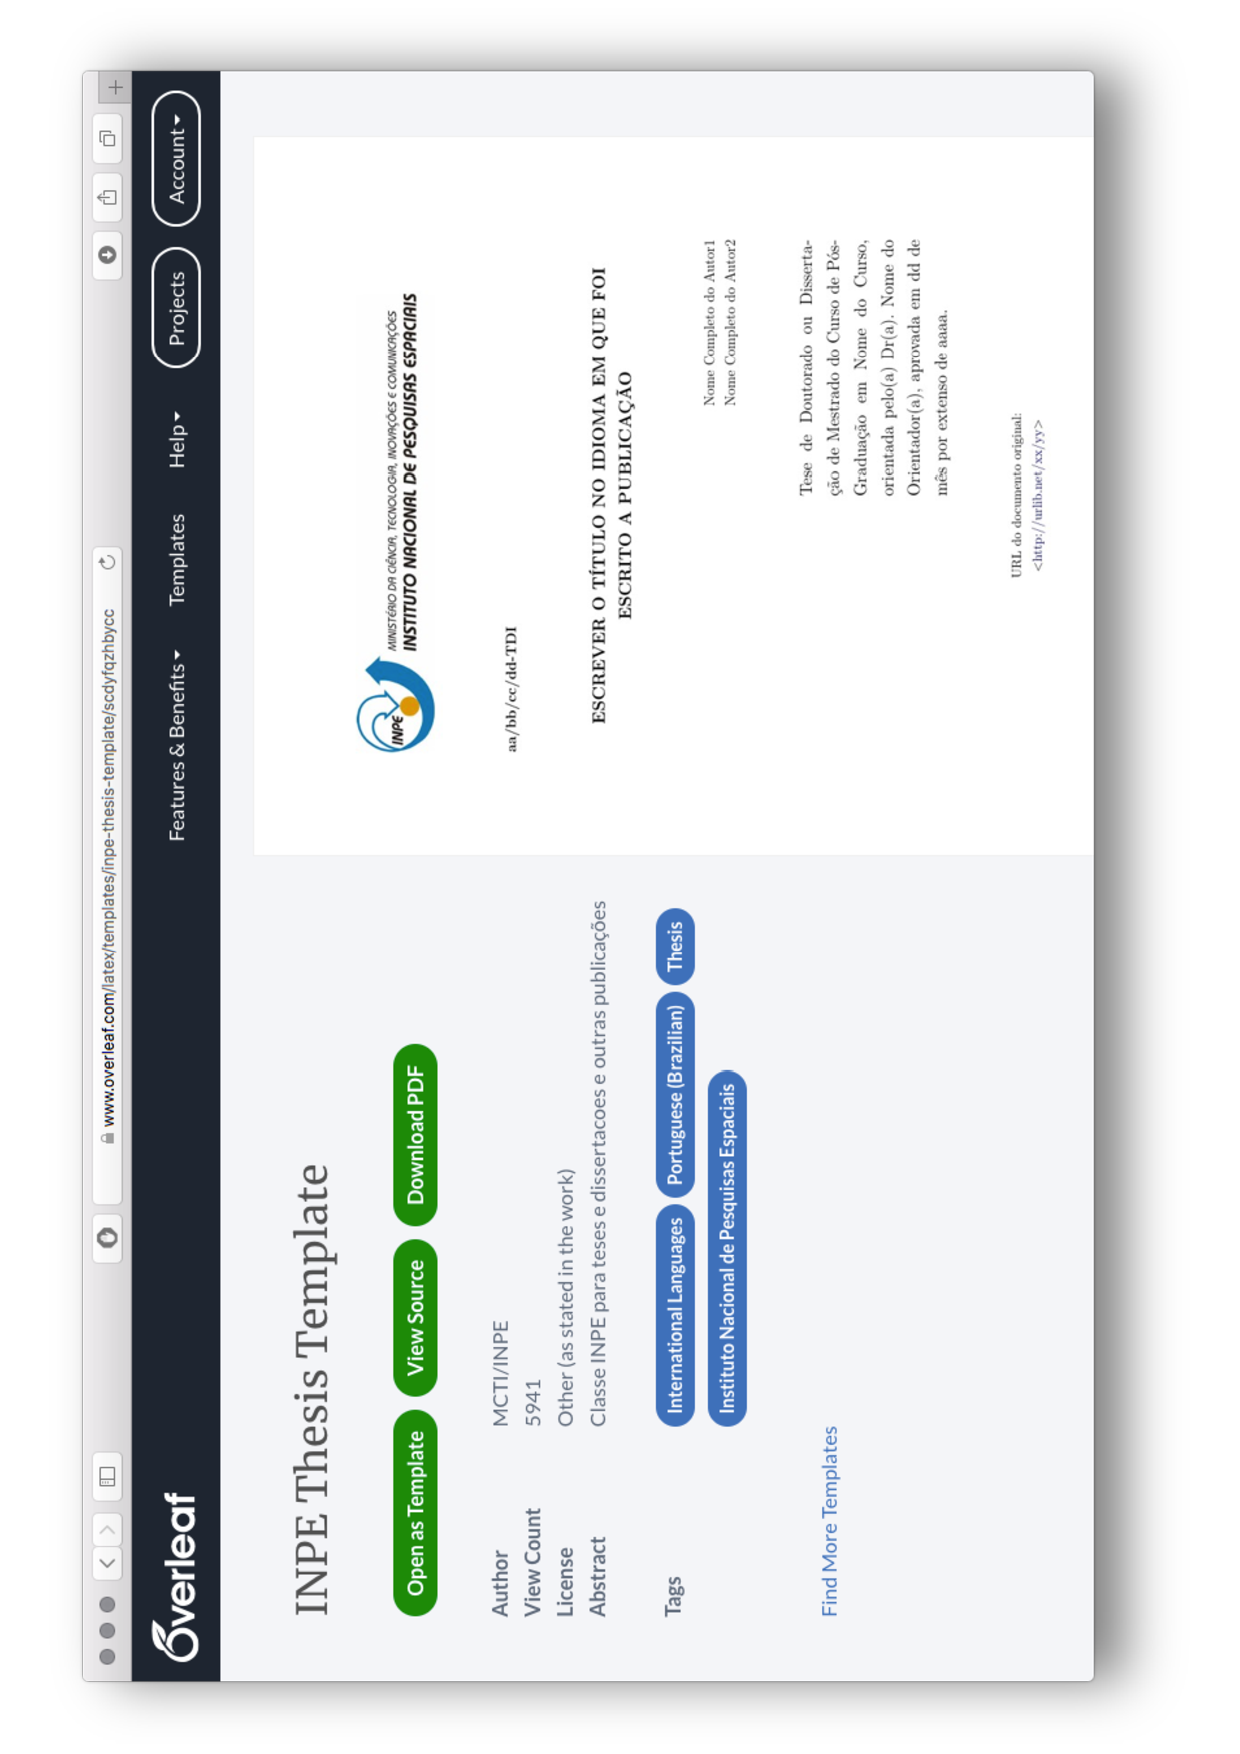
\includegraphics[width=0.7\textwidth,angle=-90]{./docs/figs/overleaf1.pdf}
  \end{center}
\vspace{4mm}
\legenda{Escolha do estilo do INPE para edição \textit{online} com o editor \textit{Overleaf}.}
\label{fig:overleaf1}
\FONTE{Produção do autor.}
\end{figure}

Na Figura \ref{fig:overleaf2} é mostrada a interface principal do editor \textit{Overleaf} com o estilo do INPE carregado para edição.

\begin{figure}[H]
\caption{O editor \textit{Overleaf}.}
\vspace{6mm}
  \begin{center}
    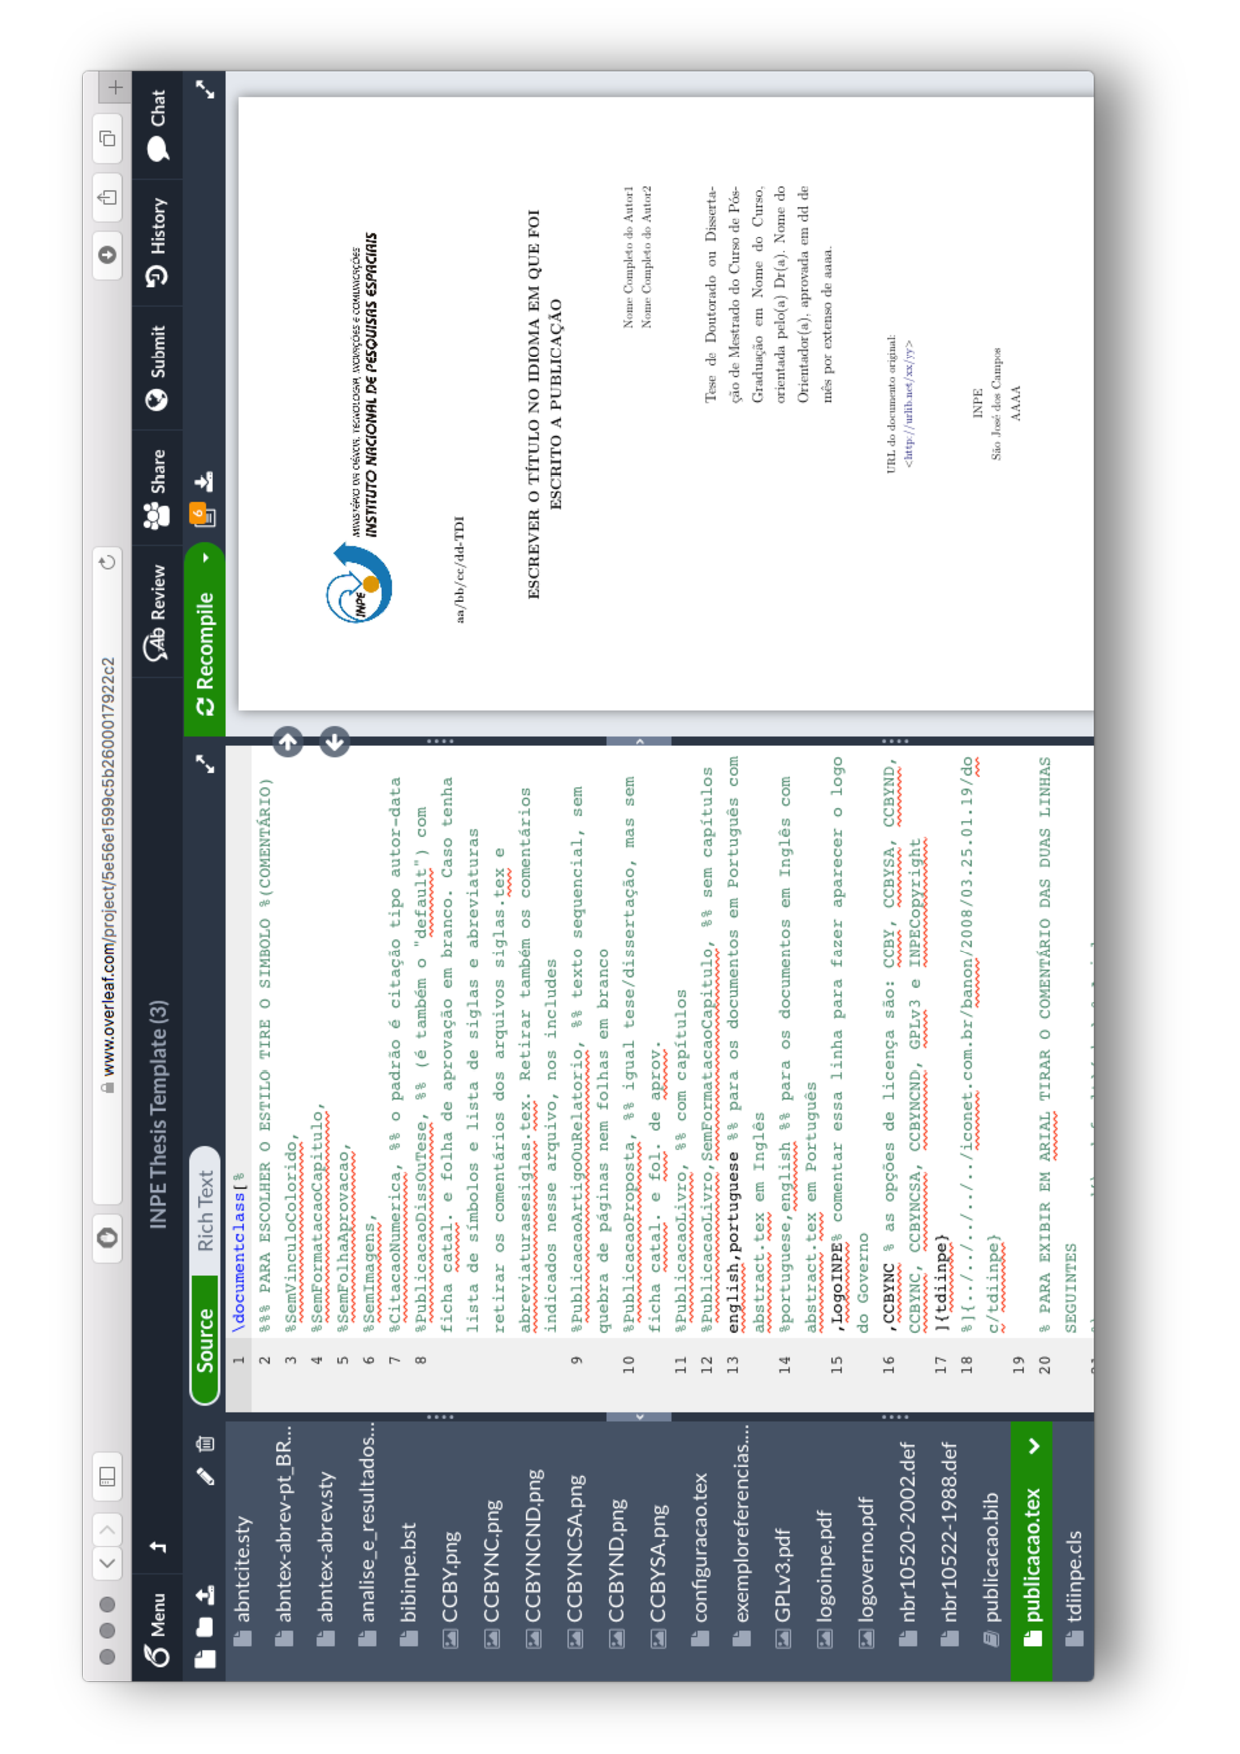
\includegraphics[width=0.7\textwidth,angle=-90]{./docs/figs/overleaf2.pdf}
  \end{center}
\vspace{4mm}
\legenda{Edição \textit{online} do estilo do INPE com o editor \textit{Overleaf}.}
\label{fig:overleaf2}
\FONTE{Produção do autor.}
\end{figure}

\begin{marker}
Ao utilizar o editor \textit{Overleaf}, o usuário irá perceber que a compilação do documento pode levar mais tempo quando muitas figuras são incluídas. Recomenda-se comentar as seções do texto que já foram revisadas para acelerar a compilação. Outra dica útil é realizar a compilação do documento no modo \textit{FAST}. Desta forma, as figuras são removidas do documento e apenas a marcadação e a estrutura do texto são compiladas.
\end{marker}

\section{Exercícios}
\label{sec:exercicios}

Para colocar em prática os comandos de marcação do \LaTeX{}, sugere-se a realização dos exercícios a seguir. Cada exercício contém um link para o Anexo A, onde estão as repostas de cada exercício. Para fazer os exercícios, você pode utilizar um editor local (instalado em seu computador) ou um editor \textit{online}, \href{https://pt.overleaf.com/project}{Overleaf}.

Para a realização dos exercícios, utilize os exemplos dados ao longo das seções do Capítulo \ref{cap:parteII}. Utilize também as tabelas do Anexo B para consultar os símbolos matemáticos pertinentes.

\tcbstartrecording

\subsection*{Marcação de Texto}
\label{sec:exec_mar_text}

Os exercícios desta seção utilizam as marcações de texto mais comuns apresentadas na Seção \ref{sec:marc_text}.

\begin{texercise}{Ex1}{Aplicando estilos diferentes de fontes}{Formate a frase abaixo utilizando os estilos {\tt textbf}, {\tt underline} e {\tt textit}}\textit{Formate a frase abaixo utilizando os estilos \mintinline{latex}{\textbf}, \mintinline{latex}{\underline}, \mintinline{latex}{\textit} e \mintinline{latex}{\sout}}:\par\smallskip%
\begin{tcboutputlisting}
\begin{center}
    A \textbf{famosa} \underline{Kelly} comeu \textit{pão infestado}
    com arroz que o \textbf{Barriga} jantou \underline{vendo} o 
    filme da \textit{Wehrmacht} \sout{xexelenta}.
\end{center}
\end{tcboutputlisting}
\tcbuselistingtext%
\end{texercise}

\begin{texercise}{Ex1a}{Aplicando cores diferentes de fontes}{Formate a frase abaixo utilizando as cores \textit{blue}, \textit{green}, \textit{red} e \textit{magenta}}\textit{Formate a frase abaixo utilizando as cores \textit{blue}, \textit{green}, \textit{red} e \textit{magenta}}:\par\smallskip%
\begin{tcboutputlisting}
\begin{center}
    A \color{blue}{famosa} \color{green}{Kelly} comeu 
    \color{red}{pão infestado} com arroz que o \color{magenta}{Barriga}
    jantou \color{blue}{vendo} o filme da \color{green}{Wehrmacht}
    \color{red}{xexelenta}.
\end{center}
\end{tcboutputlisting}
\tcbuselistingtext%
\end{texercise}

\begin{texercise}{Ex1b}{Aplicando cores de fundo diferentes}{Formate a frase abaixo utilizando as cores de fundo \textit{blue}, \textit{green}, \textit{red} e \textit{magenta}}\textit{Formate a frase abaixo utilizando as cores de fundo \textit{blue}, \textit{green}, \textit{red} e \textit{magenta}. Observe quando a cor do texto for diferente também}:\par\smallskip%
\begin{tcboutputlisting}
\begin{center}
    A \colorbox{blue}{\color{white}{famosa}} \colorbox{green}{Kelly}
    comeu \colorbox{red}{\color{white}{pão infestado}} com arroz que
    o \colorbox{magenta}{Barriga} jantou 
    \colorbox{blue}{\color{yellow}{vendo}}
    o filme da \colorbox{green}{Wehrmacht} 
    \colorbox{red}{\color{white}{xexelenta}}.
\end{center}
\end{tcboutputlisting}
\tcbuselistingtext%
\end{texercise}

\subsection*{Listas}
\label{sec:exec_listas}

Nos exercícios a seguir, utilize os exemplos mostrados na Seção \ref{sec:listas}.

\begin{texercise}{Ex2}{Criando listas simples}\textit{Crie a lista a seguir utilizando o ambiente \mintinline{latex}{itemize}}:\par\smallskip%
\begin{tcboutputlisting}
\begin{itemize}
    \item Item 1
    \begin{itemize}
        \item Item 1.1
        \item Item 1.2
    \end{itemize}
    \item Item 2
    \item Item 3
    \begin{itemize}
        \item Item 3.1
        \item Item 3.2
        \item Item 3.3
    \end{itemize}
\end{itemize}
\end{tcboutputlisting}
\tcbuselistingtext%
\end{texercise}

\begin{texercise}{Ex2a}{Criando listas simples}\textit{Crie a lista a seguir utilizando o ambiente \mintinline{latex}{enumerate}}:\par\smallskip%
\begin{tcboutputlisting}
\begin{enumerate}
    \item Item 1
    \item Item 2
    \item Item 3
\end{enumerate}
\end{tcboutputlisting}
\tcbuselistingtext%
\end{texercise}

\begin{texercise}{Ex2b}{Criando listas compostas}\textit{Crie a lista a seguir utilizando os ambientes \mintinline{latex}{enumerate} e \mintinline{latex}{itemize}}:\par\smallskip%
\begin{tcboutputlisting}
\begin{enumerate}
    \item Item 1
    \begin{itemize}
        \item Item 3.1
         \begin{enumerate}
            \item Item 3.1.1
            \begin{enumerate}
                \item Item 3.1.1.1
                \item Item 3.1.1.2
            \end{enumerate}
            \item Item 3.1.2
        \end{enumerate}
        \item Item 3.2
    \end{itemize}
\end{enumerate}
\end{tcboutputlisting}
\tcbuselistingtext%
\end{texercise}

\begin{texercise}{Ex2c}{Criando listas compostas com estilo}\textit{Crie a lista a seguir utilizando os ambientes \mintinline{latex}{enumerate} e \mintinline{latex}{itemize} e os estilos  {\tt arabic}, {\tt alph}, {\tt roman} e {\tt Alph}}:\par\smallskip%
\begin{tcboutputlisting}
\renewcommand{\labelenumi}{\arabic{enumi}}
\renewcommand{\labelenumii}{\alph{enumii}}
\renewcommand{\labelenumiii}{\roman{enumiii}}
\renewcommand{\labelenumiv}{\Alph{enumiv}}
\begin{enumerate}
    \item Item 1
    \begin{enumerate}
        \item Item 1.1
        \begin{enumerate}
            \item Item 1.1.1
            \item Item 1.1.2
        \end{enumerate}
        \item Item 1.2
    \end{enumerate}
    \item Item 2
    \item Item 3
    \begin{enumerate}
        \item Item 3.1
         \begin{enumerate}
            \item Item 3.1.1
            \begin{enumerate}
                \item Item 3.1.1.1
                \item Item 3.1.1.2
            \end{enumerate}
            \item Item 3.1.2
        \end{enumerate}
        \item Item 3.2
    \end{enumerate}
\end{enumerate}
\end{tcboutputlisting}
\tcbuselistingtext%
\end{texercise}

\subsection*{Tabelas}
\label{sec:exec_tabelas}

Nos exercícios a seguir, utilize os exemplos apresentados na Seção \ref{sec:tabs}.

\begin{texercise}{Ex3}{Criando tabelas simples}\textit{Crie a seguinte tabela utilizando o ambiente \mintinline{latex}{tabular}:}\par\smallskip%
\begin{tcboutputlisting}
\begin{tabular}{c c}
\hline
\textbf{L0C1} & \textbf{L0C2} \\
\hline
L1C1 & L1C2 \\
L2C1 & L2C2 \\
L3C1 & L3C2 \\
L4C1 & L4C2 \\
L5C1 & L5C2 \\
\hline
\end{tabular}
\end{tcboutputlisting}
\tcbuselistingtext%
\end{texercise}

\begin{texercise}{Ex3a}{Criando tabelas simples}\textit{Crie a seguinte tabela utilizando o ambiente \mintinline{latex}{tabular} e o pacote \mintinline{latex}{lipsum}:}\par\smallskip%
\begin{tcboutputlisting}
\begin{tabular}{|p{3cm}|p{3cm}|p{3cm}|p{3cm}|}
\hline
\multicolumn{4}{|c|}{4 Células Mescladas (colunas)} \\
\hline
\multicolumn{2}{|c|}{2 Células Mescladas (colunas)} &
\multicolumn{2}{c|}{2 Células Mescladas (colunas)} \\
\hline
\multicolumn{1}{|c|}{Coluna 1} &
\multicolumn{1}{c|}{Coluna 2} &
\multicolumn{1}{c|}{Coluna 3} & \multicolumn{1}{c|}{Coluna 4} \\
\hline
\lipsumsentence[1-2] & \lipsumsentence[3-4] & \lipsumsentence[5-6] &
\lipsumsentence[7-8] \\
\hline
\end{tabular}
\end{tcboutputlisting}
\tcbuselistingtext%
\end{texercise}

\begin{texercise}{Ex3b}{Criando tabelas simples}\textit{Crie a seguinte tabela utilizando o ambiente \mintinline{latex}{tabular}:}\par\smallskip%
\begin{tcboutputlisting}
\begin{tabular}{|l|c|r|}
\hline
L1C1 & L1C2 & L1C3 \\
L2C1 & L2C2 & L2C3 \\
\hline
\end{tabular}
\end{tcboutputlisting}
\tcbuselistingtext%
\end{texercise}

\begin{texercise}{Ex3c}{Criando tabelas simples}\textit{Crie a seguinte tabela utilizando o ambiente \mintinline{latex}{tabular*} e a macro {\tt textwidth}:}\par\smallskip%
\begin{tcboutputlisting}
\begin{tabular*}{\textwidth}{@{\extracolsep{\fill}}|l|c|r|}
\hline
L1C1 & L1C2 & L1C3 \\
L2C1 & L2C2 & L2C3 \\
\hline
\end{tabular*}
\end{tcboutputlisting}
\tcbuselistingtext%
\end{texercise}

%\begin{texercise}{Ex3c}{Criando tabelas simples}\textit{Crie a seguinte tabela utilizando o ambiente \mintinline{latex}{tabular} e a macro {\tt textwidth}:}\par\smallskip%
%\begin{tcboutputlisting}
%\begin{tabular}{\textwidth}{|X|X|X|}
%\hline
%L1C1 & L1C2 & L1C3 \\
%L2C1 & L2C2 & L2C3 \\
%\hline
%\end{tabular}
%\end{tcboutputlisting}
%\tcbuselistingtext%
%\end{texercise}

\begin{texercise}{Ex3d}{Criando tabelas simples}\textit{Crie a seguinte tabela utilizando o ambiente \mintinline{latex}{tabular} e os separadores especiais {\tt toprule}, {\tt midrule} e {\tt bottomrule}:}\par\smallskip%
\begin{tcboutputlisting}
\begin{tabular}[t]{lcc}
\toprule
     & L1C2 & L1C3 \\
\midrule
L2C1 & L2C2 & L2C3 \\
L3C1 & L3C2 & L3C3 \\
L4C1 & L4C2 & L4C3 \\
\bottomrule
\end{tabular}
\end{tcboutputlisting}
\tcbuselistingtext%
\end{texercise}

%\subsection*{Macros com 1 parâmetro}
%\label{sec:exec_macros_1_par}
%
%Nas seções a seguir, crie macros simples para a substituição de palavras ou expressões. Utilize os exemplos da Seção \ref{sec:macros}.
%
%%\begin{texercise}{Ex4}{Criando macros com 1 parâmetro}\textit{Crie uma nova macro \verb+\headingline+ que produza o seguinte resultado}:\par\smallskip%
%%    \begin{tcboutputlisting}
%%        \newcommand{\headingline}[1]{%
%%            \begin{center}\Large\bfseries #1\end{center}}
%%        \end{tcboutputlisting}
%%
%%        \tcbuselistingtext%
%%
%%Crie uma nova macro \verb+\headingline+ que produza o seguinte resultado:\par\smallskip
%%
%%    \begin{tcbwritetemp}
%%        \headingline{Título muito importante}
%%    \end{tcbwritetemp}
%%    \tcbusetemplisting\tcbusetemp%
%%\end{texercise}
%%
%%\subsection*{Macros com 2 parâmetros}
%%\label{sec:exec_macros_2_par}
%%
%%\begin{texercise}{Ex5}{Criando macros com 2 parâmetros}{Crie uma nova macro \verb+\minitable+ que produza o seguinte resultado}:\par\smallskip
%%\begin{tcboutputlisting}
%%\newcommand{\minitable}[2]{%
%%    \begin{center}\begin{tabular}{p{10cm}}\hline%
%%    \multicolumn{1}{c}{\bfseries#1}\\\hline%
%%    #2\\\hline%
%%    \end{tabular}\end{center}}
%%    \end{tcboutputlisting}
%%    \tcbuselistingtext%
%%    Crie uma nova macro \verb+\minitable+ que produza o seguinte resultado:\par\smallskip\begin{tcbwritetemp}
%%    \minitable{Meu título}{Nesta pequena tabela, há apenas 
%%    um título e algum texto abaixo com largura de dez centímetros.}
%%    \end{tcbwritetemp}
%%    \tcbusetemplisting\par\smallskip\tcbusetemp%
%%\end{texercise}
%
\subsection*{Matemática e Equações}
\label{sec:exec_mat_eqs}

Nos seguintes exercícios, utilize os exemplos apresentados na Seção \ref{sec:mat_eqs} e as tabelas do Anexo A.

\begin{texercise}{Ex_Eq1}{Matrizes sem delimitadores}\textit{Uma matriz sem delimitadores ({\tt matrix})}:\par\smallskip%
\begin{tcboutputlisting}
    \begin{center}
        \begin{equation*}
            X = 
            \begin{matrix} 
                x_{11} & x_{12} & x_{13} \\ 
                x_{21} & x_{22} & x_{23} \\ 
                x_{31} & x_{32} & x_{33} 
            \end{matrix}
        \end{equation*}
    \end{center}
\end{tcboutputlisting}
\tcbuselistingtext%
\end{texercise}

\begin{texercise}{Ex_Eq2}{Matrizes com delimitadores quadrados}\textit{Uma matriz com delimitadores quadrados ({\tt bmatrix})}:\par\smallskip%
\begin{tcboutputlisting}
    \begin{center}
        \begin{equation*}
            X =
            \begin{bmatrix} 
                x_{11} & x_{12} & x_{13} \\ 
                x_{21} & x_{22} & x_{23} \\ 
                x_{31} & x_{32} & x_{33} 
            \end{bmatrix}
        \end{equation*}
    \end{center}
\end{tcboutputlisting}
\tcbuselistingtext%
\end{texercise}

\begin{texercise}{Ex_Eq3}{Matrizes com delimitadores curvos}\textit{Uma matriz com delimitadores curvos ({\tt pmatrix})}:\par\smallskip%
\begin{tcboutputlisting}
    \begin{center}
        \begin{equation*}
            X =
            \begin{pmatrix} 
                x_{11} & x_{12} & x_{13} \\ 
                x_{21} & x_{22} & x_{23} \\ 
                x_{31} & x_{32} & x_{33} 
            \end{pmatrix}
        \end{equation*}
    \end{center}
\end{tcboutputlisting}
\tcbuselistingtext%
\end{texercise}

\begin{texercise}{Ex_Eq4}{Matrizes com delimitadores verticais}\textit{Uma matriz com delimitadores verticais simples ({\tt vmatrix})}:\par\smallskip%
\begin{tcboutputlisting}
    \begin{center}
        \begin{equation*}
            X =
            \begin{vmatrix} 
                x_{11} & x_{12} & x_{13} \\ 
                x_{21} & x_{22} & x_{23} \\ 
                x_{31} & x_{32} & x_{33} 
            \end{vmatrix}
        \end{equation*}
    \end{center}
\end{tcboutputlisting}
\tcbuselistingtext%
\end{texercise}

\begin{texercise}{Ex_Eq5}{Matrizes com delimitadores verticais duplos}\textit{Uma matriz com delimitadores verticais duplos ({\tt Vmatrix})}:\par\smallskip%
\begin{tcboutputlisting}
    \begin{center}
        \begin{equation*}
            X =
            \begin{Vmatrix} 
                x_{11} & x_{12} & x_{13} \\ 
                x_{21} & x_{22} & x_{23} \\ 
                x_{31} & x_{32} & x_{33} 
            \end{Vmatrix}
        \end{equation*}
    \end{center}
\end{tcboutputlisting}
\tcbuselistingtext%
\end{texercise}

\begin{texercise}{Ex_Eq6}{Matrizes delimitadas por chaves}\textit{Uma matriz delimitada por chaves ({\tt Bmatrix})}:\par\smallskip%
\begin{tcboutputlisting}
    \begin{center}
        \begin{equation*}
            X =
            \begin{Bmatrix} 
                x_{11} & x_{12} & x_{13} \\ 
                x_{21} & x_{22} & x_{23} \\ 
                x_{31} & x_{32} & x_{33} 
            \end{Bmatrix}
        \end{equation*}
    \end{center}
\end{tcboutputlisting}
\tcbuselistingtext%
\end{texercise}

%\begin{texercise}{Ex_Eq7}{Expressões com limites}\textit{A definição da derivada de uma função contínua em $x$}:\par\smallskip%
%\begin{tcboutputlisting}
%    \begin{center}
%        \begin{equation*}
%            \frac{df(x)}{dx} = \lim_{x \to 0}{\frac{f(x + h) - f(x)}{h}}
%        \end{equation*}
%    \end{center}
%\end{tcboutputlisting}
%\tcbuselistingtext%
%\end{texercise}

%\begin{texercise}{Ex_Eq3}{Expressões entre parênteses}\textit{Utilize \mintinline{latex}{(} e \mintinline{latex}{)} para delimitar uma expressão arbitrária entre parênteses}:\par\smallskip%
%\begin{tcboutputlisting}
%    \begin{center}
%        \begin{equation*}
%            \left( \frac{p}{q} \right)
%        \end{equation*}
%    \end{center}
%\end{tcboutputlisting}
%\tcbuselistingtext%
%\end{texercise}

\begin{texercise}{Ex_Eq7}{Expressões com limites}\textit{A derivada $f'(a)$ da função $f(x)$ no ponto $x=a$ é o limite}:\par\smallskip%
\begin{tcboutputlisting}
    \begin{center}
        \begin{equation*}
            f'(a) = \lim_{x \to a} \frac{f(x) - f(a)}{x - a}
        \end{equation*}
    \end{center}
\end{tcboutputlisting}
\tcbuselistingtext%
\end{texercise}

\begin{texercise}{Ex_Eq8}{Expressões com limites}\textit{A função $f(x)$ é contínua no ponto $x=a$ se}:\par\smallskip%
\begin{tcboutputlisting}
    \begin{center}
        \begin{equation*}
            \lim_{x \to a^{-}} f(x) = f(a) = \lim_{x \to a^{+}} f(x)
        \end{equation*}
    \end{center}
\end{tcboutputlisting}
\tcbuselistingtext%
\end{texercise}

\begin{texercise}{Ex_Eq9}{Expressões séries algébricas}\textit{A série de MacLaurin para $e^{x}$ é}:\par\smallskip%
\begin{tcboutputlisting}
    \begin{center}
        \begin{equation*}
            e^{x} = \sum_{k=0}^{\infty} \frac{x^{k}}{k!}
        \end{equation*}
    \end{center}
\end{tcboutputlisting}
\tcbuselistingtext%
\end{texercise}

%\begin{texercise}{Ex_Eq7}{Escrevendo matrizes de derivadas}\textit{A matriz Jacobiano da função \(\mathbf{f}(x_1, \dots, x_n)\) é}:\par\smallskip%
%\begin{tcboutputlisting}
%    \begin{center}
%        \begin{equation*}
%            \mathbf{J}
%            =
%            \frac{d \mathbf{f}}{d \mathbf{x}}
%            =
%            \left[ \frac{\partial \mathbf{f}}{\partial x_1}
%            \cdots \frac{\partial \mathbf{f}}{\partial x_n} \right]
%            =
%            \begin{bmatrix}
%            \frac{\partial f_1}{\partial x_1} & \cdots &
%            \frac{\partial f_1}{\partial x_n} \\
%            \vdots & \ddots & \vdots \\
%            \frac{\partial f_m}{\partial x_1} & \cdots &
%            \frac{\partial f_m}{\partial x_n}
%            \end{bmatrix}
%        \end{equation*}
%    \end{center}
%\end{tcboutputlisting}
%\tcbuselistingtext%
%\end{texercise}

\begin{texercise}{Ex_Eq10}{Expressões trigonométricas}\textit{Identidade da soma de dois ângulos é}:\par\smallskip%
\begin{tcboutputlisting}
    \begin{center}
        \begin{equation*}
            \text{cos}(\alpha \pm \beta) = 
            \text{cos }\alpha \text{ cos }\beta \mp 
            \text{ sin }\alpha \text{ sin }\beta
        \end{equation*}
    \end{center}
\end{tcboutputlisting}
\tcbuselistingtext%
\end{texercise}

\begin{texercise}{Ex_Eq11}{Expressões com integrais}\textit{A integral indefinida de $\frac{1}{a+x^{2}}$ é}:\par\smallskip%
\begin{tcboutputlisting}
    \begin{center}
        \begin{equation*}
            \int \frac{1}{a+x^{2}}dx = \text{arctan } x + C
        \end{equation*}
    \end{center}
\end{tcboutputlisting}
\tcbuselistingtext%
\end{texercise}

\begin{texercise}{Ex_Eq12}{Expressões com divergente}\textit{E equação de Navier-Stokes para um fluxo incompressível é}:\par\smallskip%
\begin{tcboutputlisting}
    \begin{center}
        \begin{equation*}
            \frac{\partial{\mathbf{u}}}{\partial{t}} + 
            (\mathbf{u} \cdot \nabla)\mathbf{u} - 
            \nu \nabla^2 \mathbf{u} = - \nabla \omega + \mathbf{g}
        \end{equation*}
    \end{center}
\end{tcboutputlisting}
\tcbuselistingtext%
\end{texercise}

\begin{texercise}{Ex_Eq13}{Equações diferenciais}\textit{O Teorema de Green é dado por}:\par\smallskip%
\begin{tcboutputlisting}
    \begin{center}
        \begin{equation*}
            \oint_C (Ldx + Mdy) = \iint_D \bigg(\frac{\partial{M}}
            {\partial{x}} - \frac{\partial{L}}{\partial{y}}\bigg)dxdy
        \end{equation*}
    \end{center}
\end{tcboutputlisting}
\tcbuselistingtext%
\end{texercise}

\begin{texercise}{Ex_Eq14}{Equações diferenciais}\textit{A Equação de Poisson é}:\par\smallskip%
\begin{tcboutputlisting}
    \begin{center}
        \begin{equation*}
            \frac{\partial^{2}\Psi}{\partial x^{2}} +
            \frac{\partial^{2}\Psi}{\partial y^{2}} = G(x,y)
        \end{equation*}
    \end{center}
\end{tcboutputlisting}
\tcbuselistingtext%
\end{texercise}

\begin{texercise}{Ex_Eq15}{Equações diferenciais}\textit{A Equação de Laplace é}:\par\smallskip%
\begin{tcboutputlisting}
    \begin{center}
        \begin{equation*}
            \frac{\partial^{2}\Psi}{\partial x^{2}} + 
            \frac{\partial^{2}\Psi}{\partial y^{2}} = 0
        \end{equation*}
    \end{center}
\end{tcboutputlisting}
\tcbuselistingtext%
\end{texercise}

\begin{texercise}{Ex_Eq16}{Equações diferenciais}\textit{A Equação de Fourier (ou da condução do calor) é}:\par\smallskip%
\begin{tcboutputlisting}
    \begin{center}
        \begin{equation*}
            \frac{\partial^{2}\Psi}{\partial x^{2}} -
            k\frac{\partial\Psi}{\partial y} = 0
        \end{equation*}
    \end{center}
\end{tcboutputlisting}
\tcbuselistingtext%
\end{texercise}

\begin{texercise}{Ex_Eq17}{Equações diferenciais}\textit{A Equação de D'Alembert (ou da onda) é}:\par\smallskip%
\begin{tcboutputlisting}
    \begin{center}
        \begin{equation*}
            \frac{\partial^{2}\Psi}{\partial x^{2}} - 
            k^{2}\frac{\partial^{2}\Psi}{\partial y^{2}} = 0
        \end{equation*}
    \end{center}
\end{tcboutputlisting}
\tcbuselistingtext%
\end{texercise}

\begin{texercise}{Ex_Eq18}{Expressões com limites e logaritmos}\textit{O Teorema dos Números Primos é dado por}:\par\smallskip%
\begin{tcboutputlisting}
    \begin{center}
        \begin{equation*}
            \lim_{x \to \infty} 
            \frac{\pi(x)}{\frac{x}{\text{log}(x)}} = 1
        \end{equation*}
    \end{center}
\end{tcboutputlisting}
\tcbuselistingtext%
\end{texercise}

\begin{texercise}{Ex_Eq19}{Expressões com somatórios}\textit{A fórmula geral da série de Taylor é}:\par\smallskip%
\begin{tcboutputlisting}
    \begin{center}
        \begin{equation*}
            \sum_{n=0}^{\infty} \frac{f^{(n)}(a)}{n!}(x-a)^n
        \end{equation*}
    \end{center}
\end{tcboutputlisting}
\tcbuselistingtext%
\end{texercise}

\begin{texercise}{Ex_Eq20}{Expressões com integrais e derivadas}\textit{O Teorema de Stokes é dado por}:\par\smallskip%
\begin{tcboutputlisting}
    \begin{center}
        \begin{equation*}
            \int_{\partial{\Omega}} \omega = \int_{\Omega} d\omega
        \end{equation*}
    \end{center}
\end{tcboutputlisting}
\tcbuselistingtext%
\end{texercise}

\begin{texercise}{Ex_Eq21}{Expressões com produto tensorial}\textit{A propriedade adjunta do produto tensorial é}:\par\smallskip%
\begin{tcboutputlisting}
    \begin{center}
        \begin{equation*}
            \text{Hom}(U \otimes V, W) \cong 
            \text{Hom}(U, \text{Hom}(V,W))
        \end{equation*}
    \end{center}
\end{tcboutputlisting}
\tcbuselistingtext%
\end{texercise}
  
\begin{texercise}{Ex_Eq22}{Expressões com a transformada de Laplace}\textit{A definição da transformada de Laplace é dada por}:\par\smallskip%
\begin{tcboutputlisting}
    \begin{center}
        \begin{equation*}
            \mathcal{L} \lbrace f(t) \rbrace = 
            F(s) \int_{0}^{\infty} f(t) e^{-st} dt
        \end{equation*}
    \end{center}
\end{tcboutputlisting}
\tcbuselistingtext%
\end{texercise}
  
\begin{texercise}{Ex_Eq23}{Equações matriciais}\textit{A fórmula da inversa de uma matriz é}:\par\smallskip%
\begin{tcboutputlisting}
    \begin{center}
        \begin{equation*}
            \begin{bmatrix}
                x_{11} & x_{12} \\
                x_{21} & x_{22} \\
            \end{bmatrix}^{-1} 
            = \frac{1}{x_{11}x_{22} - x_{12}x_{21}} 
            \begin{bmatrix}
                x_{22} & -x_{12}  \\
                -x_{21} &  x_{11} \\
            \end{bmatrix}
        \end{equation*}
    \end{center}
\end{tcboutputlisting}
\tcbuselistingtext%
\end{texercise}
  
\begin{texercise}{Ex_Eq24}{Expressões com parênteses maiores}\textit{A fórmula do produto infinito pode ser escrita como}:\par\smallskip%
\begin{tcboutputlisting}
    \begin{center}
        \begin{equation*}
            \text{sin }x = x \prod^{\infty}_{n=1} 
            \bigg(1 - \frac{x^2}{\pi^{2} n^{2}} \bigg)
        \end{equation*}
    \end{center}
\end{tcboutputlisting}
\tcbuselistingtext%
\end{texercise}

%\subsection*{Documentos Simples}
%\label{sec:docs_simples}
%
%\begin{texercise}{Ex_Doc1}{Um documento simples completo}\textit{Reproduza o documento a seguir, utilizando os seguintes pacotes
%\begin{itemize}
%\item {\tt babel}, com a opção {\tt brazilian}
%\item {\tt inputenc} com a opção {\tt utf8}
%\item {\tt fontenc} com a opção {\tt T1}
%\item {\tt lipsum}
%\item {\tt booktabs}
%\item {\tt graphicx}
%\item {\tt float}
%\item {\tt tabularx}
%\end{itemize}
%}:\par\smallskip%
%\begin{tcboutputlisting}
%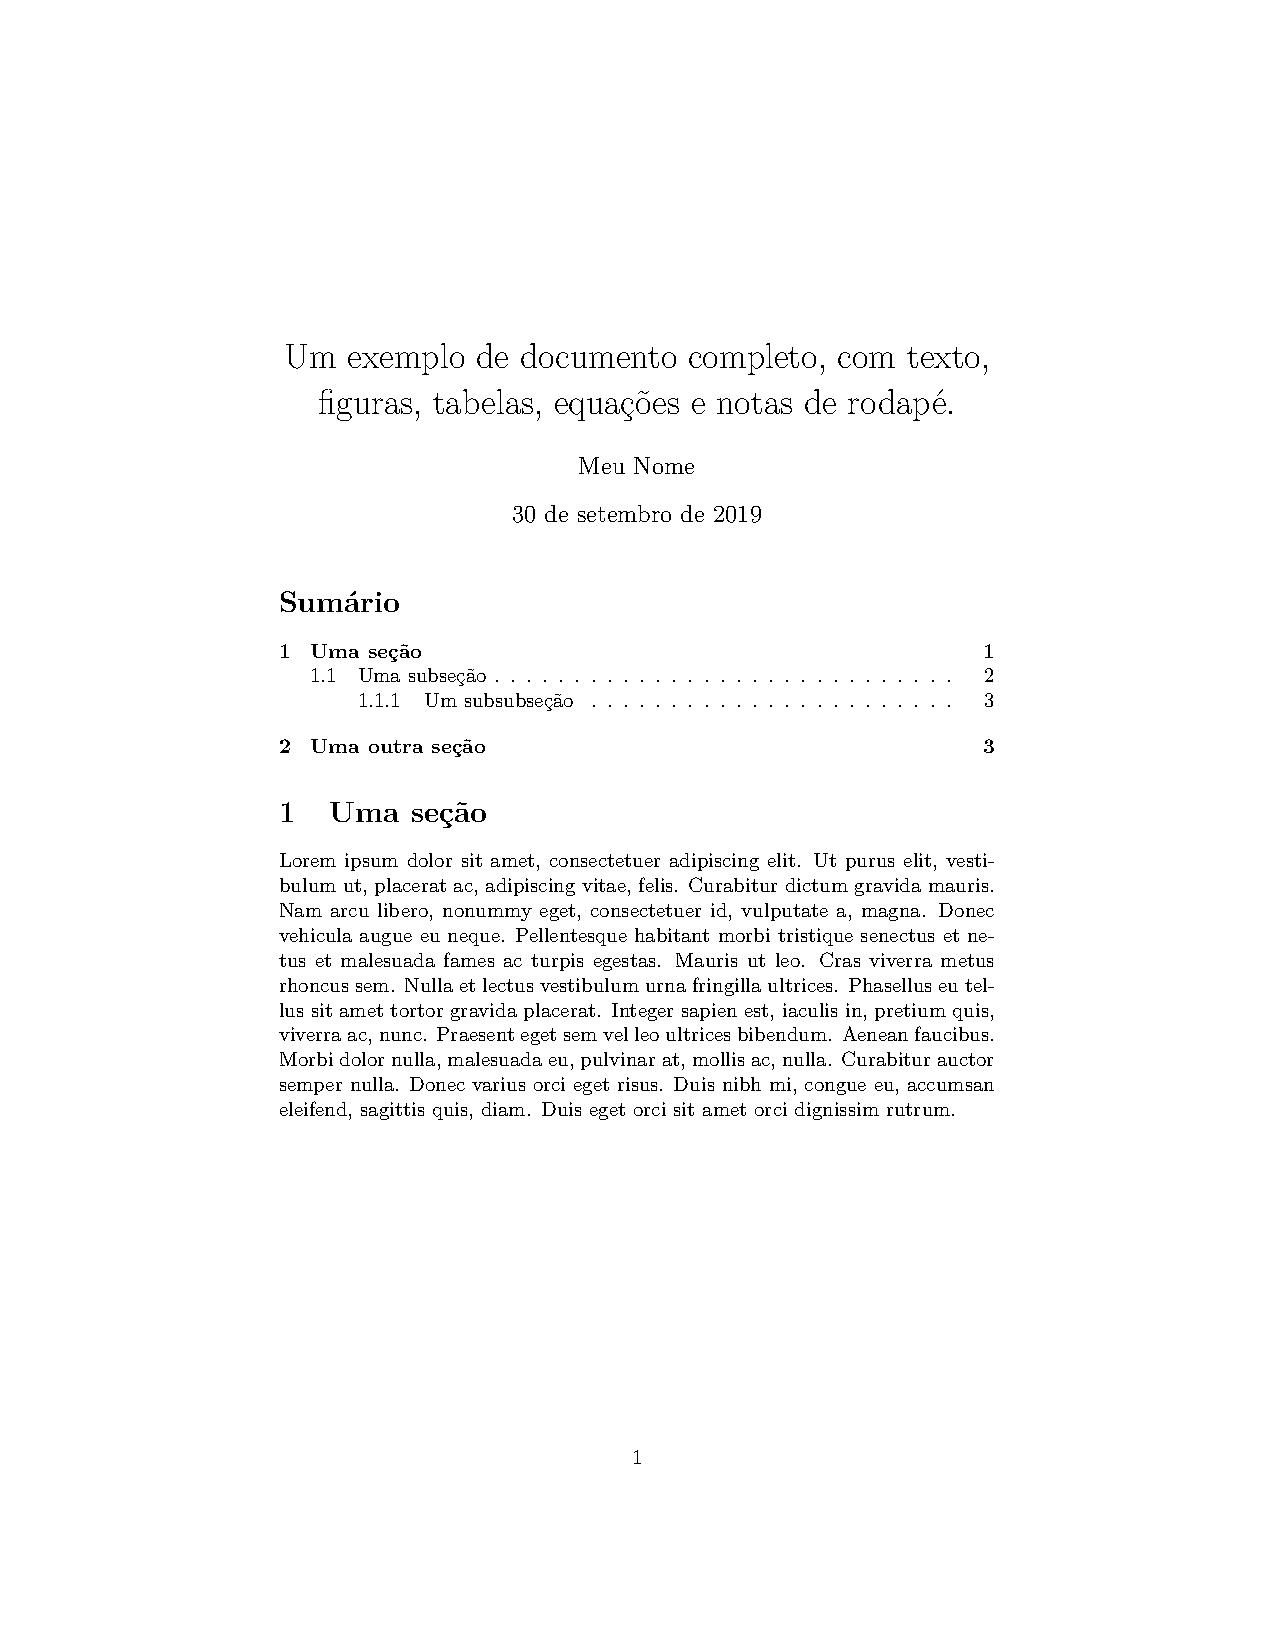
\includepdf[pages=-]{completo.pdf}
%\end{tcboutputlisting}
%\tcbuselistingtext%
%\end{texercise}

\tcbstoprecording

\chapter{Parte III - Estilo do INPE}
\label{cap:parteIII}

O INPE desenvolveu um estilo próprio para a publicação de teses, dissertações e relatórios. Este estilo está disponível para edição na linguagem de marcação \LaTeX{}, além dos editores WYSIWYG \textit{Microsoft Word} e \textit{LibreOffice}. Este capítulo trata da aplicação do estilo do INPE no ambiente da linguagem de marcação \LaTeX{}.

\section{Estilo do INPE para Dissertações e Teses}

O estilo do INPE compreende um conjunto de arquivos que contém instruções e imagens, que permitem que os documentos escritos dentro do seu escopo, sejam montados segundo as normas de publicação do Serviço de Informação e Documentação (SESID) do INPE. O estilo do INPE foi originalmente criado por \citeonline{roth/2002}, e tem sido mantido e atualizado desde 2002 por diversos colaboradores do INPE. Veja na seção a seguir como obter uma cópia do estilo do INPE. %A versão mais atualizada do estilo pode ser sempre encontrada no endereço \url{http://mtc-m16c.sid.inpe.br/col/iconet.com.br/banon/2008/03.25.01.19/doc/tdiinpe.cls}.

\subsection*{Obtendo o Estilo}
\label{sec:obter}

É possível obter uma cópia do estilo do INPE a partir de duas formas distintas. A primeira, é entrar no \textit{site} da biblioteca do INPE, a partir do endereço \url{http://www.inpe.br/biblioteca/}. Na página, no menu lateral, clique em ``Como Publicar?'' e depois em ``em \LaTeX{}'' (Figura \ref{fig:biblio_pub_latex}). Na página, no \textit{frame} da direita, uma outra página irá se abrir com as instruções ``Publicar usando estilo em \LaTeX{}''. A página contém instruções sobre todo o processo de publicação de documentos submetidos à revisão pelo SESID. Para obter uma cópia \textit{offline} do pacote com o estilo do INPE em \LaTeX{}, clique no \textit{link} \href{http://mtc-m16c.sid.inpe.br/archive.cgi/sid.inpe.br/iris@1905/2005/08.25.14.01}{``download do estilo baixando o arquivo archive.zip''} que está na ``OPÇÃO 3 (compilação no próprio computador)''. Na mesma página, há instruções sobre a instalação de um compilador \LaTeX{}, que também podem ser encontradas no Capítulo \ref{cap:parteI} deste documento.

%\begin{figure}[H]
%    \centering
%    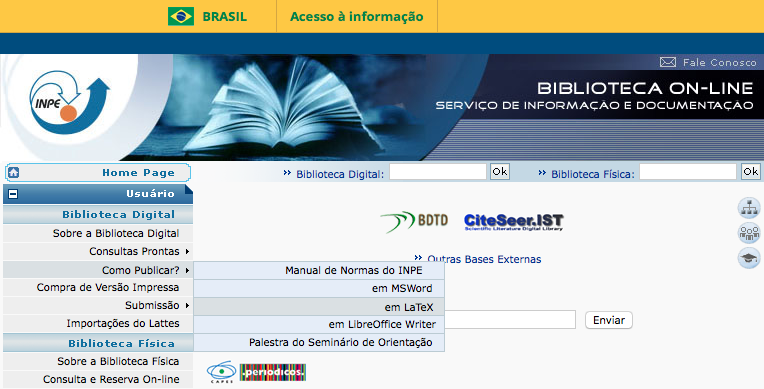
\includegraphics[scale=0.5]{./docs/figs/biblio_pub_latex.png}
%    \caption{Obtenção do estilo \LaTeX{} do INPE a partir do \textit{site} da Biblioteca do INPE.}
%    \label{fig:biblio_pub_latex}
%\end{figure}

\begin{figure}[H]
\caption{Obtenção do estilo \LaTeX{} do INPE a partir do \textit{site} da Biblioteca do INPE.}
\vspace{6mm}
    \begin{center}
        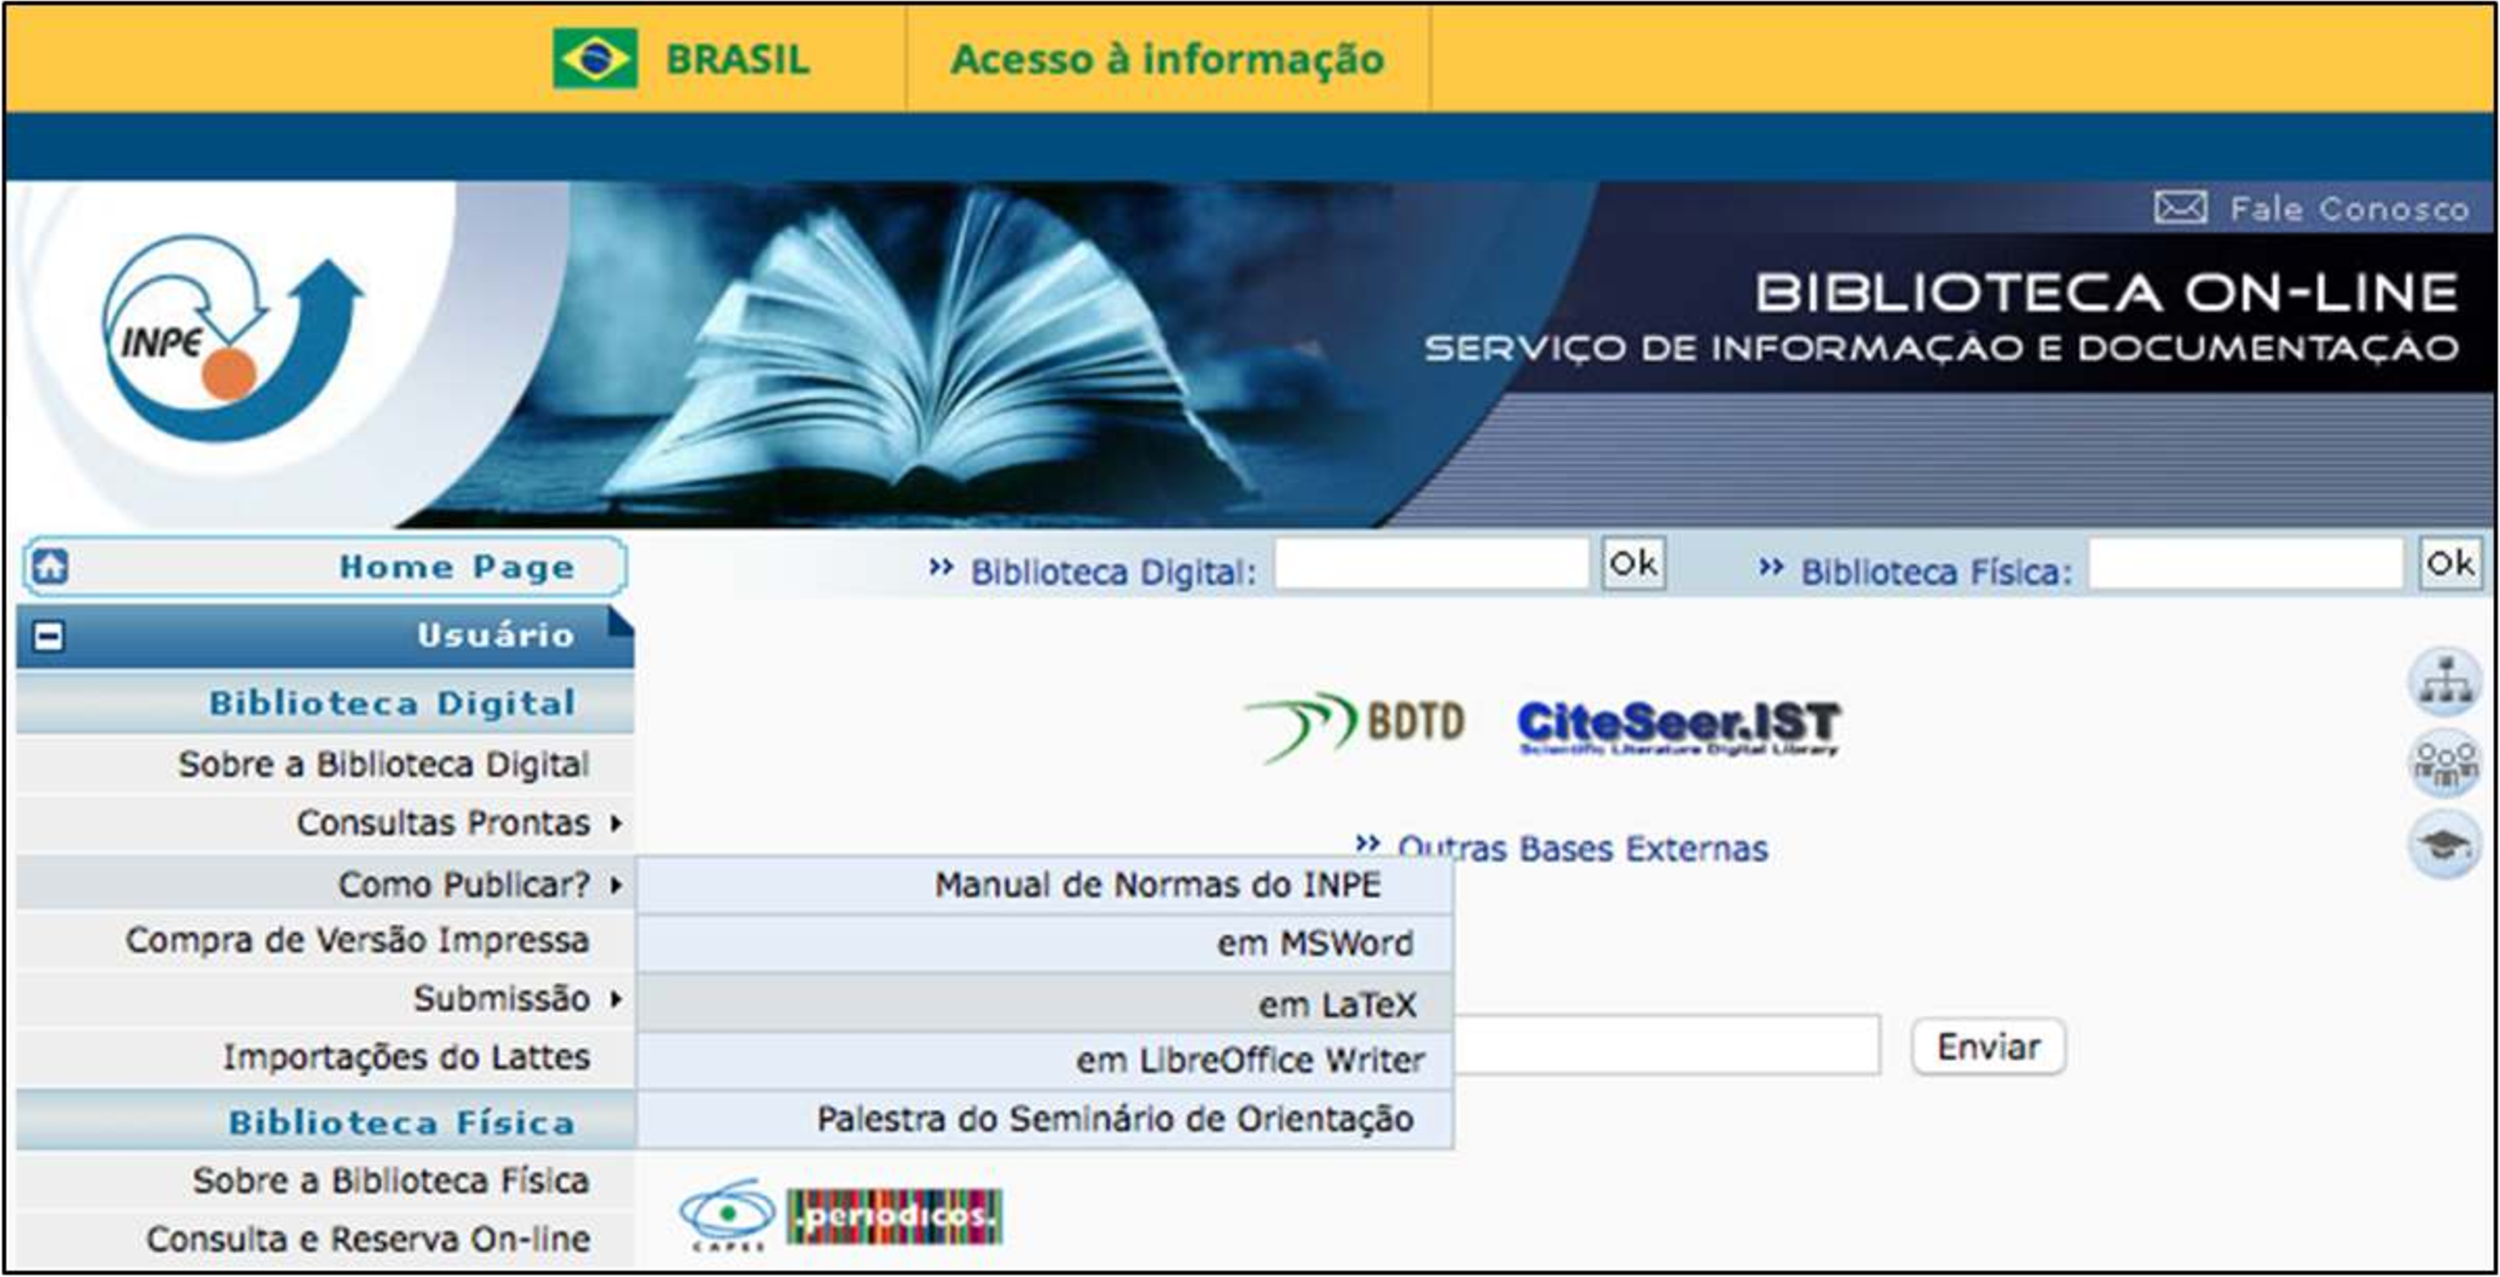
\includegraphics[scale=0.3]{./docs/figs/biblio_pub_latex.pdf}
    \end{center}
\vspace{4mm}
\legenda{\textit{Site} do biblioteca do INPE.}
\label{fig:biblio_pub_latex}
\FONTE{Produção do autor.}
\end{figure}

Com o arquivo {\tt archive.zip} no seu computador, descompacte-o em um local apropriado para poder ter acesso aos arquivos que compõem o estilo do INPE.

%\subsection{Conhecendo a estrutura e ambiente (arquivos que compõem o modelo, preenchimento de dados básicos, dicas práticas sobre o que se pode e o que não se pode fazer na hora de utilizar o modelo do INPE)}

\subsection{Estrutura e Organização}
\label{sec:estrut}

O estilo do INPE é fornecido pelo arquivo principal {\tt tdiinpe.cls}. Dentro deste arquivo há uma série de instruções da linguagem \LaTeX{} que determinam o estilo das referências, dos capítulos, dos títulos, tabelas, imagens etc (Figura \ref{fig:estrut}).

%\begin{figure}[H]
%    \centering
%    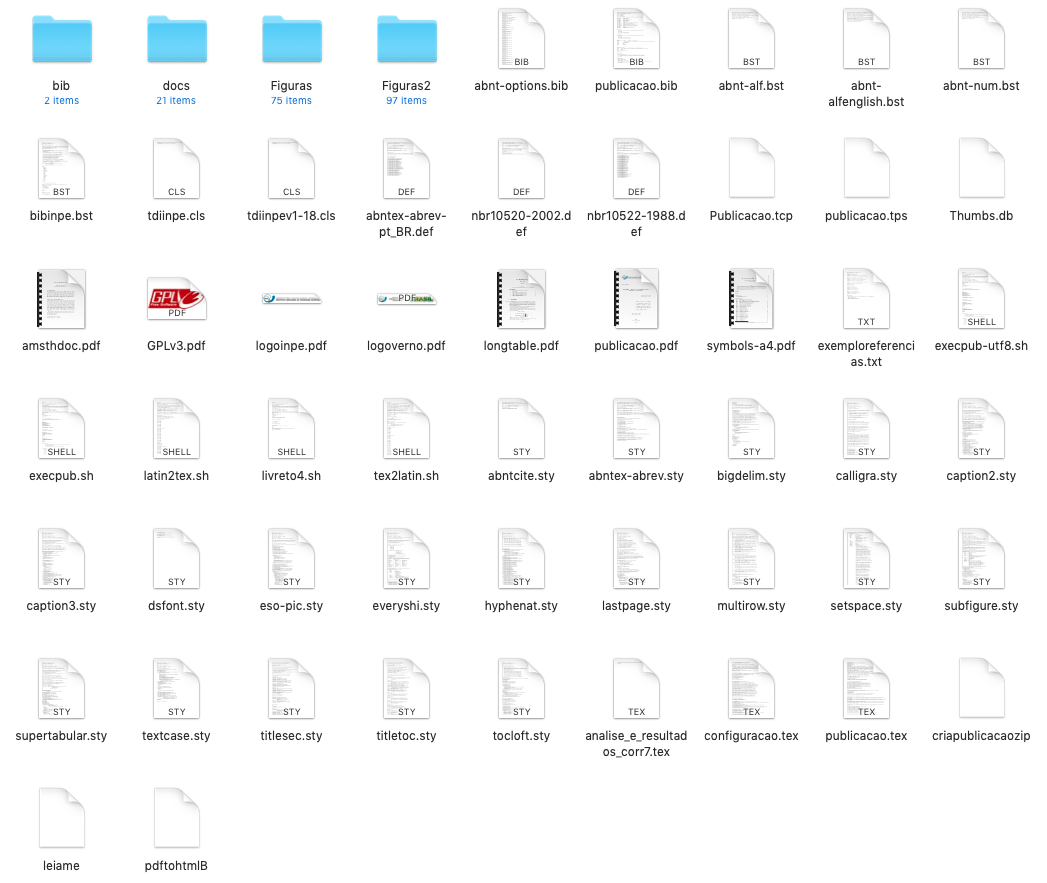
\includegraphics[scale=0.4]{./docs/figs/estrutura_estilo_inpe.png}
%    \caption{Estrutura e organização do estilo \LaTeX{} do INPE.}
%    \label{fig:estrut}
%\end{figure}

\begin{figure}[H]
\caption{Estrutura e organização do estilo \LaTeX{} do INPE.}
\vspace{6mm}
    \begin{center}
        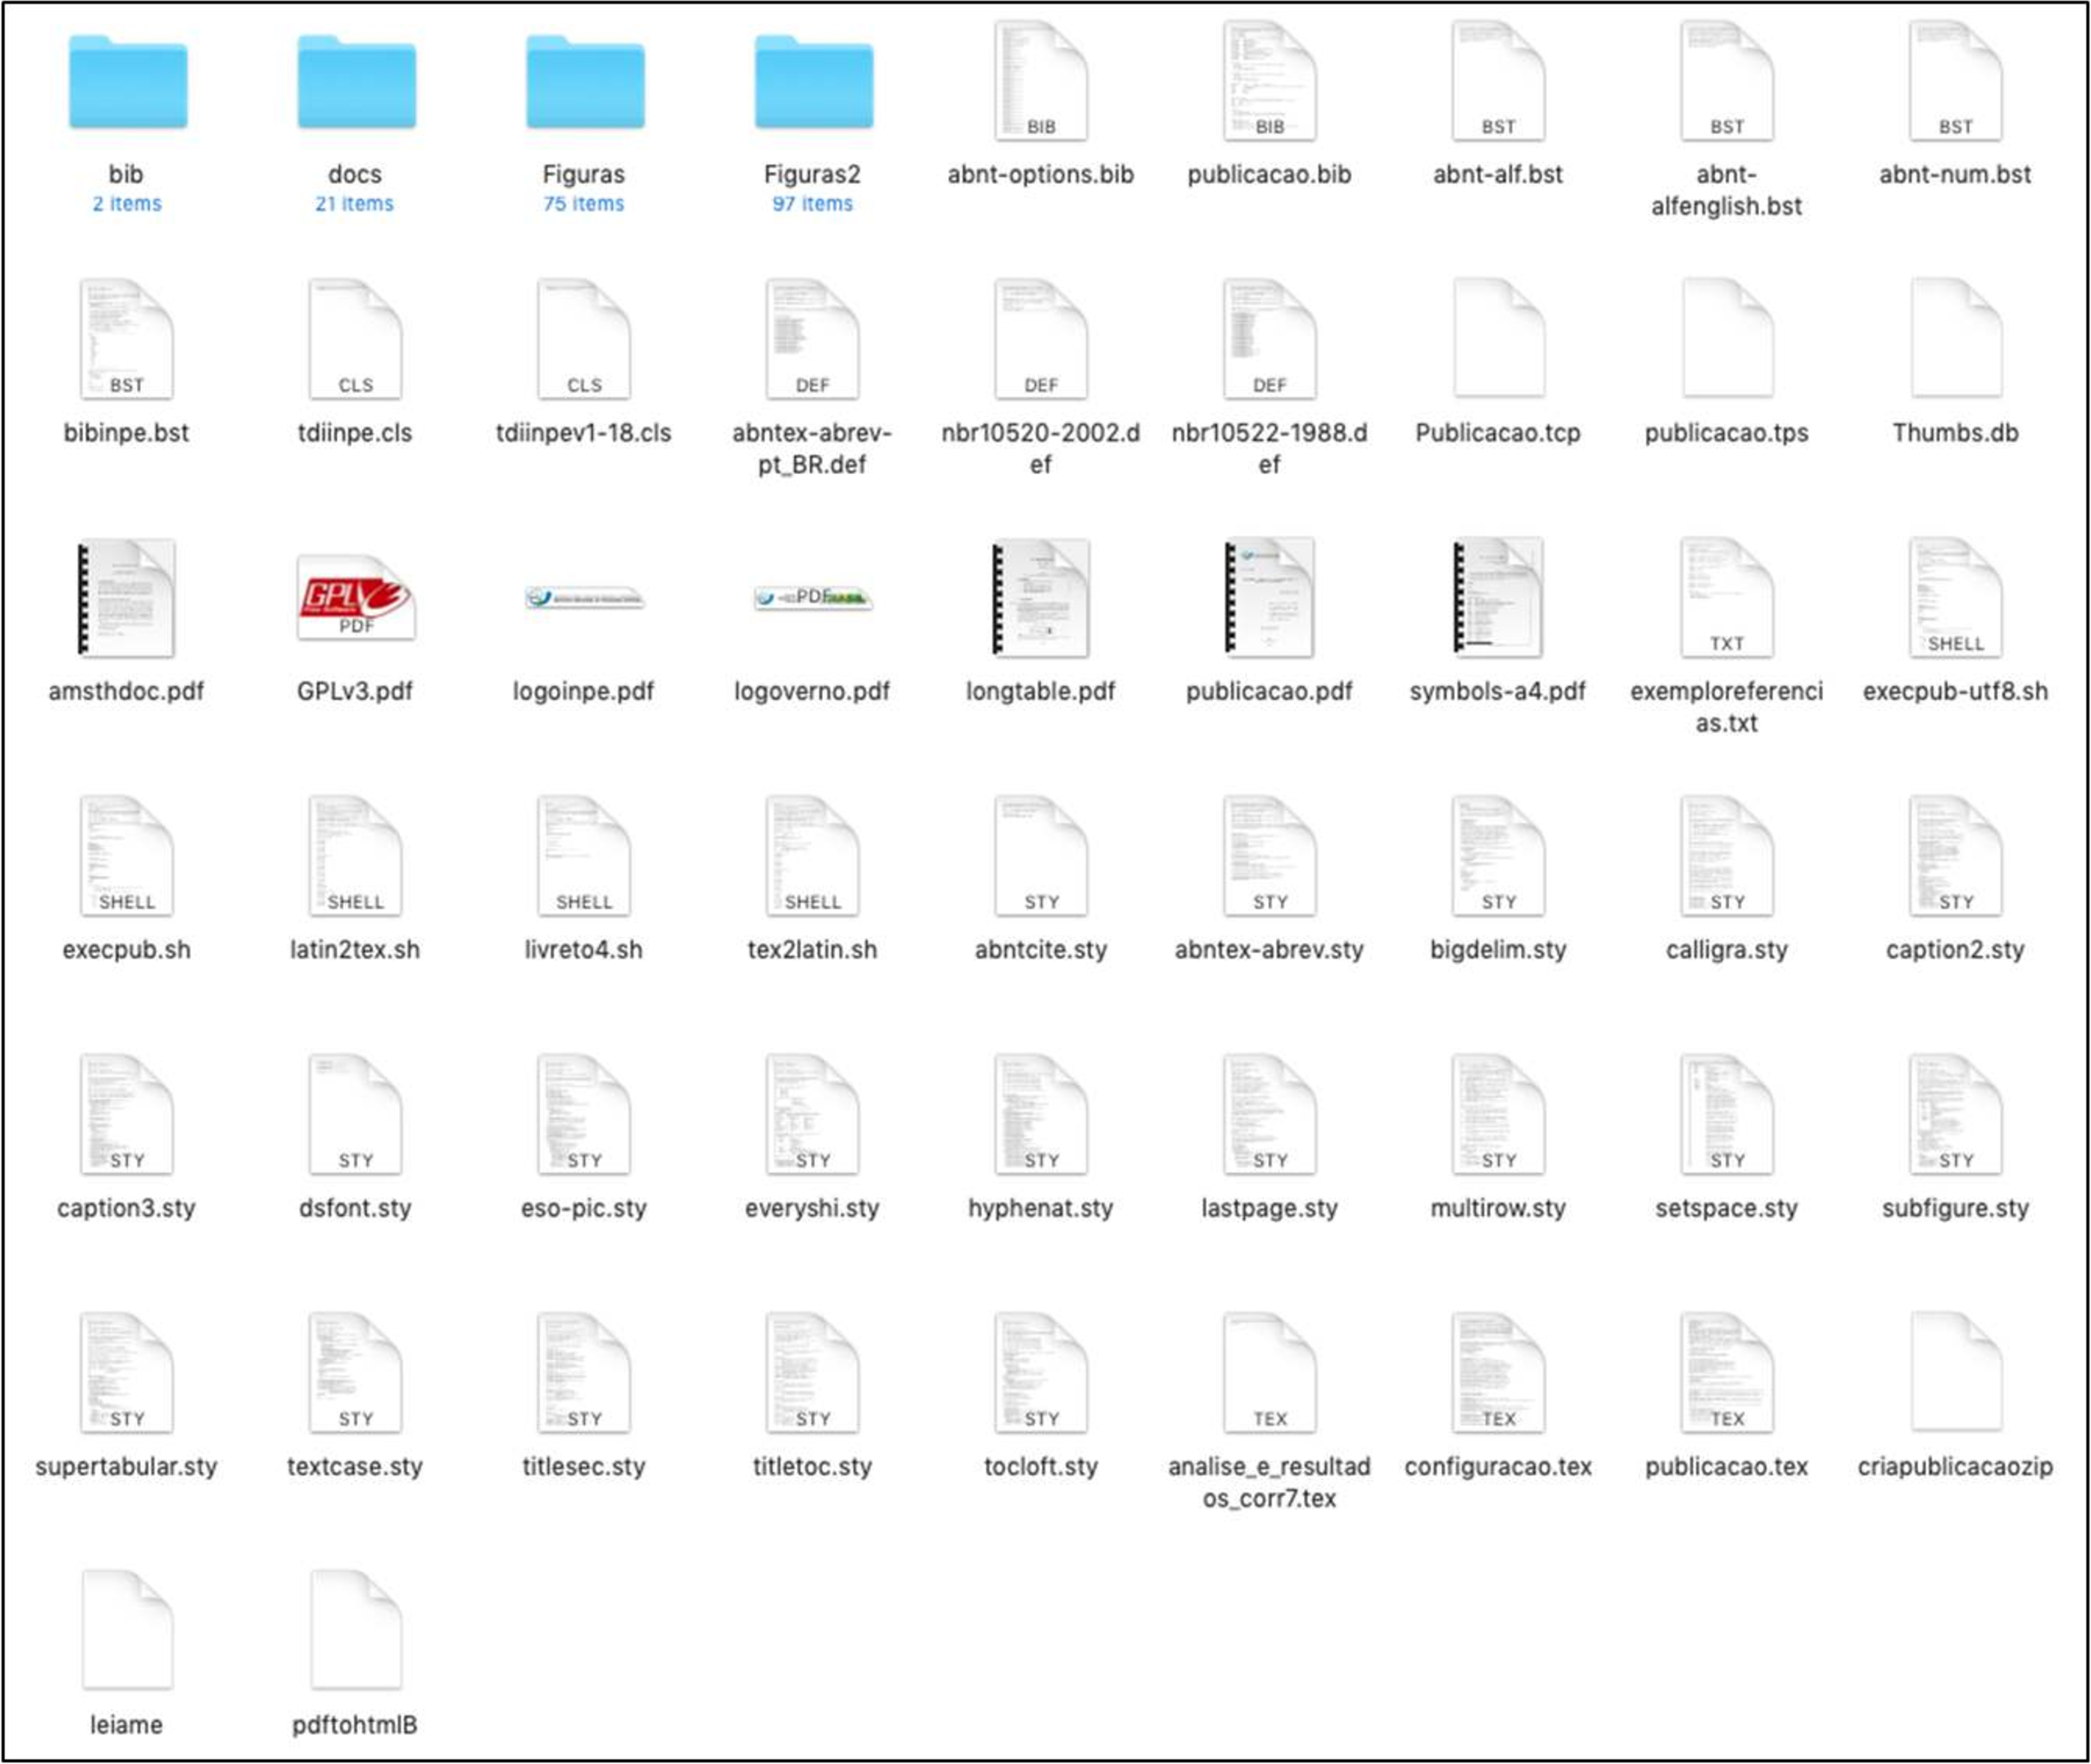
\includegraphics[scale=0.3]{./docs/figs/estrutura_estilo_inpe.pdf}
    \end{center}
\vspace{4mm}
\legenda{Arquivos do estilo \LaTeX{} do INPE.}
\label{fig:estrut}
\FONTE{Produção do autor.}
\end{figure}

Na Figura \ref{fig:estrut}, os arquivos da estrutura do estilo do INPE estão misturados aos arquivos do documento em si. Outros arquivos são resultados do processo de compilação do documento principal. 

\begin{multicols}{2}
    \textbf{Diretórios}
    \begin{itemize}
        \item bib/
        \item Figuras/
        \item docs/
    \end{itemize}
    \textbf{Arquivos do Estilo}
    \begin{itemize}
        \color{MaterialBlue}{\item leiame
        \item GPLv3.pdf
        \item CCBY.png
        \item CCBYNC.png
        \item CCBYNCND.png
        \item CCBYNCSA.png
        \item CCBYND.png
        \item CCBYSA.png
        \item logoverno.pdf
        \item logoinpe.pdf
        \item tdiinpe.cls}                                                        
        \color{MaterialRed}{\item abntex-abrev-pt\_BR.def      
        \item abntex-abrev.sty
        \item nbr10520-2002.def
        \item nbr10522-1988.def
        \item abnt-alf.bst
        \item abnt-alfenglish.bst
        \item bibinpe.bst
        \item eso-pic.sty
        \item abnt-num.bst
        \item abnt-options.bib
		\item abntcite.sty}
    \end{itemize}
	\textbf{Outros Pacotes Fornecidos}
	\begin{itemize}
        \item caption2.sty
        \item calligra.sty
        \item caption3.sty
		\item hyphenat.sty
		\item multirow.sty    
        \item dsfont.sty
		\item supertabular.sty
		\item tocloft.sty   
        \item setspace.sty
		\item titlesec.sty   
        \item textcase.sty
		\item lastpage.sty     
        \item bigdelim.sty
		\item everyshi.sty 
        \item subfigure.sty
		\item titletoc.sty
	\end{itemize}
	\textbf{Arquivos de Configuração}
	\begin{itemize}
		\item configuracao.tex
	\end{itemize}
    \textbf{Arquivos de Documentos}
    \begin{itemize}
        \item publicacao.tex
    \end{itemize}
    \textbf{\textit{Scripts}}
    \begin{itemize}
        \item tex2latin.sh
        \item criapublicacaozip
        \item latin2tex.sh
        \item pdftohtmlB
        \item livreto4.sh
        \item execpub.sh
    \end{itemize}
    \textbf{Documento Final}
    \begin{itemize}
        \item publicacao.pdf
    \end{itemize}
\end{multicols}

Na lista de arquivos acima, observe que a lista ``Arquivos do Estilo'', há arquivos destacados nas cores azul e vermelho. Os arquivos em azul, representam os arquivos do estilo do INPE, enquanto que os arquivos em vermelho, representam os arquivos do estilo de citação da ABNT. O arquivo final gerado é o arquivo {\tt publicacao.pdf}. O documento principal do pacote, também chamado de \textit{master}, é o arquivo {\tt publicacao.tex}; o arquivo que contém as configurações principais do documento (e.g., título, autor, banca e datas) é o arquivo {\tt configuracao.tex} e o arquivo que contém as diretivas do estilo do INPE é o {\tt tdiinpe.cls}. Em geral, não é necessário editar o arquivo de estilo, a não ser que exista algum conflito em relação a pacotes e versões (veja um exemplo na Seção \ref{sec:oriesp}). 

\subsection{Compilação do Documento}
\label{sec:compilacao}

Para compilar o documento é necessário ter algum compilador o \LaTeX{} instalado localmente ou utilizar algum serviço \textit{online} como o \href{https://www.overleaf.com/}{Overleaf}. No \textit{Overleaf}, o \textit{link} para a edição do estilo em sua versão atual é \url{https://www.overleaf.com/latex/templates/inpe-thesis-template/scdyfqzhbycc#.Wrj8gH8h2Uk}. Para a compilação local, recomenda-se a utilização dos \textit{scripts} que se encontram na distribuição:

\begin{itemize}
    \item \textbf{criapublicacaozip}: \textit{script} que empacota o documento final ({\tt publicacao.pdf}) para publicação;
    \item \textbf{latin2tex.sh}: \textit{script} que converte acentos latinos para a marcação da linguagem \LaTeX{}\footnote{Não obrigatório dependendo da opção do pacote {\tt inputenc}.};
    \item \textbf{tex2latin.sh}: \textit{script} que converte acentos com marcação \LaTeX{} para acentos latinos\footnote{Idem comentário anterior.};
    \item \textbf{pdftohtmlB}: converte um documento PDF em HTML;
    \item \textbf{livreto4.sh}: gera um livreto de quatro folhas no formato A4\footnote{O formato livreto pode ser útil para prova de impressão.};
    \item \textbf{execpub.sh}: gera o documento de saída ({\tt publicacao.pdf}) utilizando o compilador \LaTeX{}\footnote{Veja mais detalhes sobre o processo de compilação de um documento \LaTeX{} na Seção \ref{sec:intro_latex} do Capítulo \ref{cap:parteII}}. 
\end{itemize}

Para compilar um documento utilizando o estilo do INPE e o conjunto de \textit{scripts} fornecidos, siga os seguintes passos:

\textbf{1.} Abra um terminal\footnote{No sistema operacional \textit{Microsoft Windows 10}, recomenda-se a utilização de qualquer distribuição Linux, instalada através do Subsistema \textit{Windows} para Linux (SWL). Veja como instalar em \url{https://docs.microsoft.com/pt-br/windows/wsl/install-win10}.} e navegue até o diretório onde se encontra o \textit{script} {\tt execpub.sh};

\textbf{2.} Altere a permissão de execução do \textit{script} {\tt execpub.sh} com o comando:

\begin{meucomando}
chmod +x execpub.sh
\end{meucomando}

\textbf{3.} Execute o \textit{script} {\tt execpub.sh} sem argumentos. Na Figura \ref{fig:execpub} são mostrados as opções do \textit{script} {\tt execpub.sh}: 

%\begin{figure}[H]
%    \centering
%    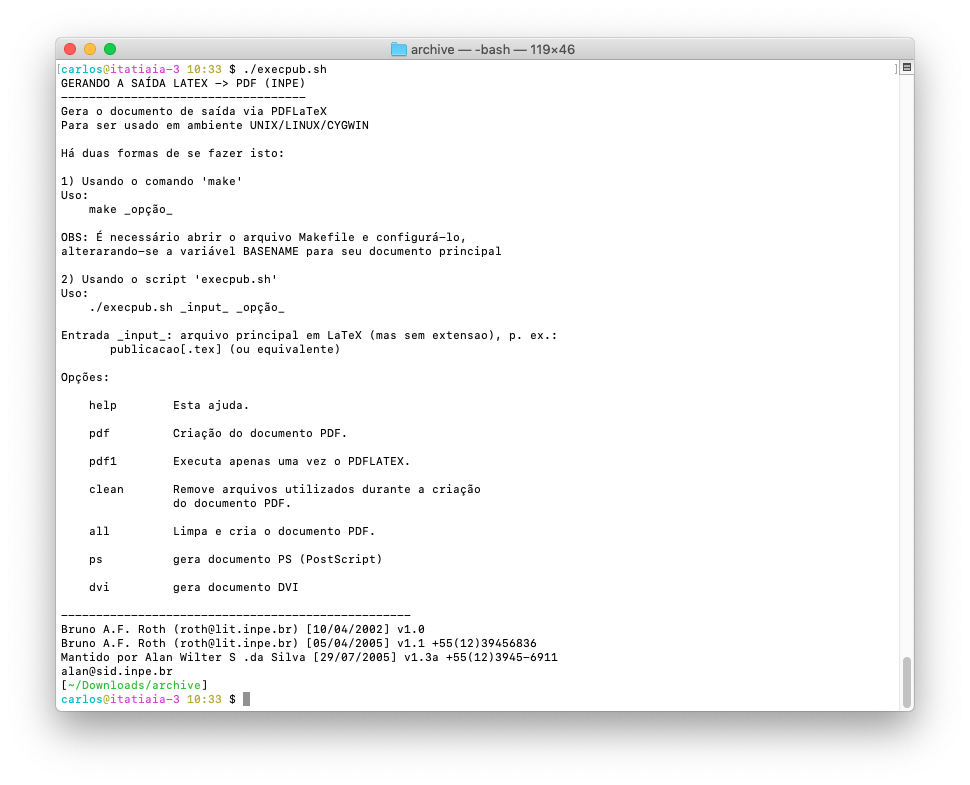
\includegraphics[scale=0.4]{./docs/figs/saida_execpub.png}
%    \caption{Exemplo de execução do \textit{script} {\tt execpub.sh} sem argumentos.}
%    \label{fig:execpub}
%\end{figure}

\begin{figure}[H]
\caption{Exemplo de execução do \textit{script} {\tt execpub.sh} sem argumentos.}
\vspace{6mm}
    \begin{center}
        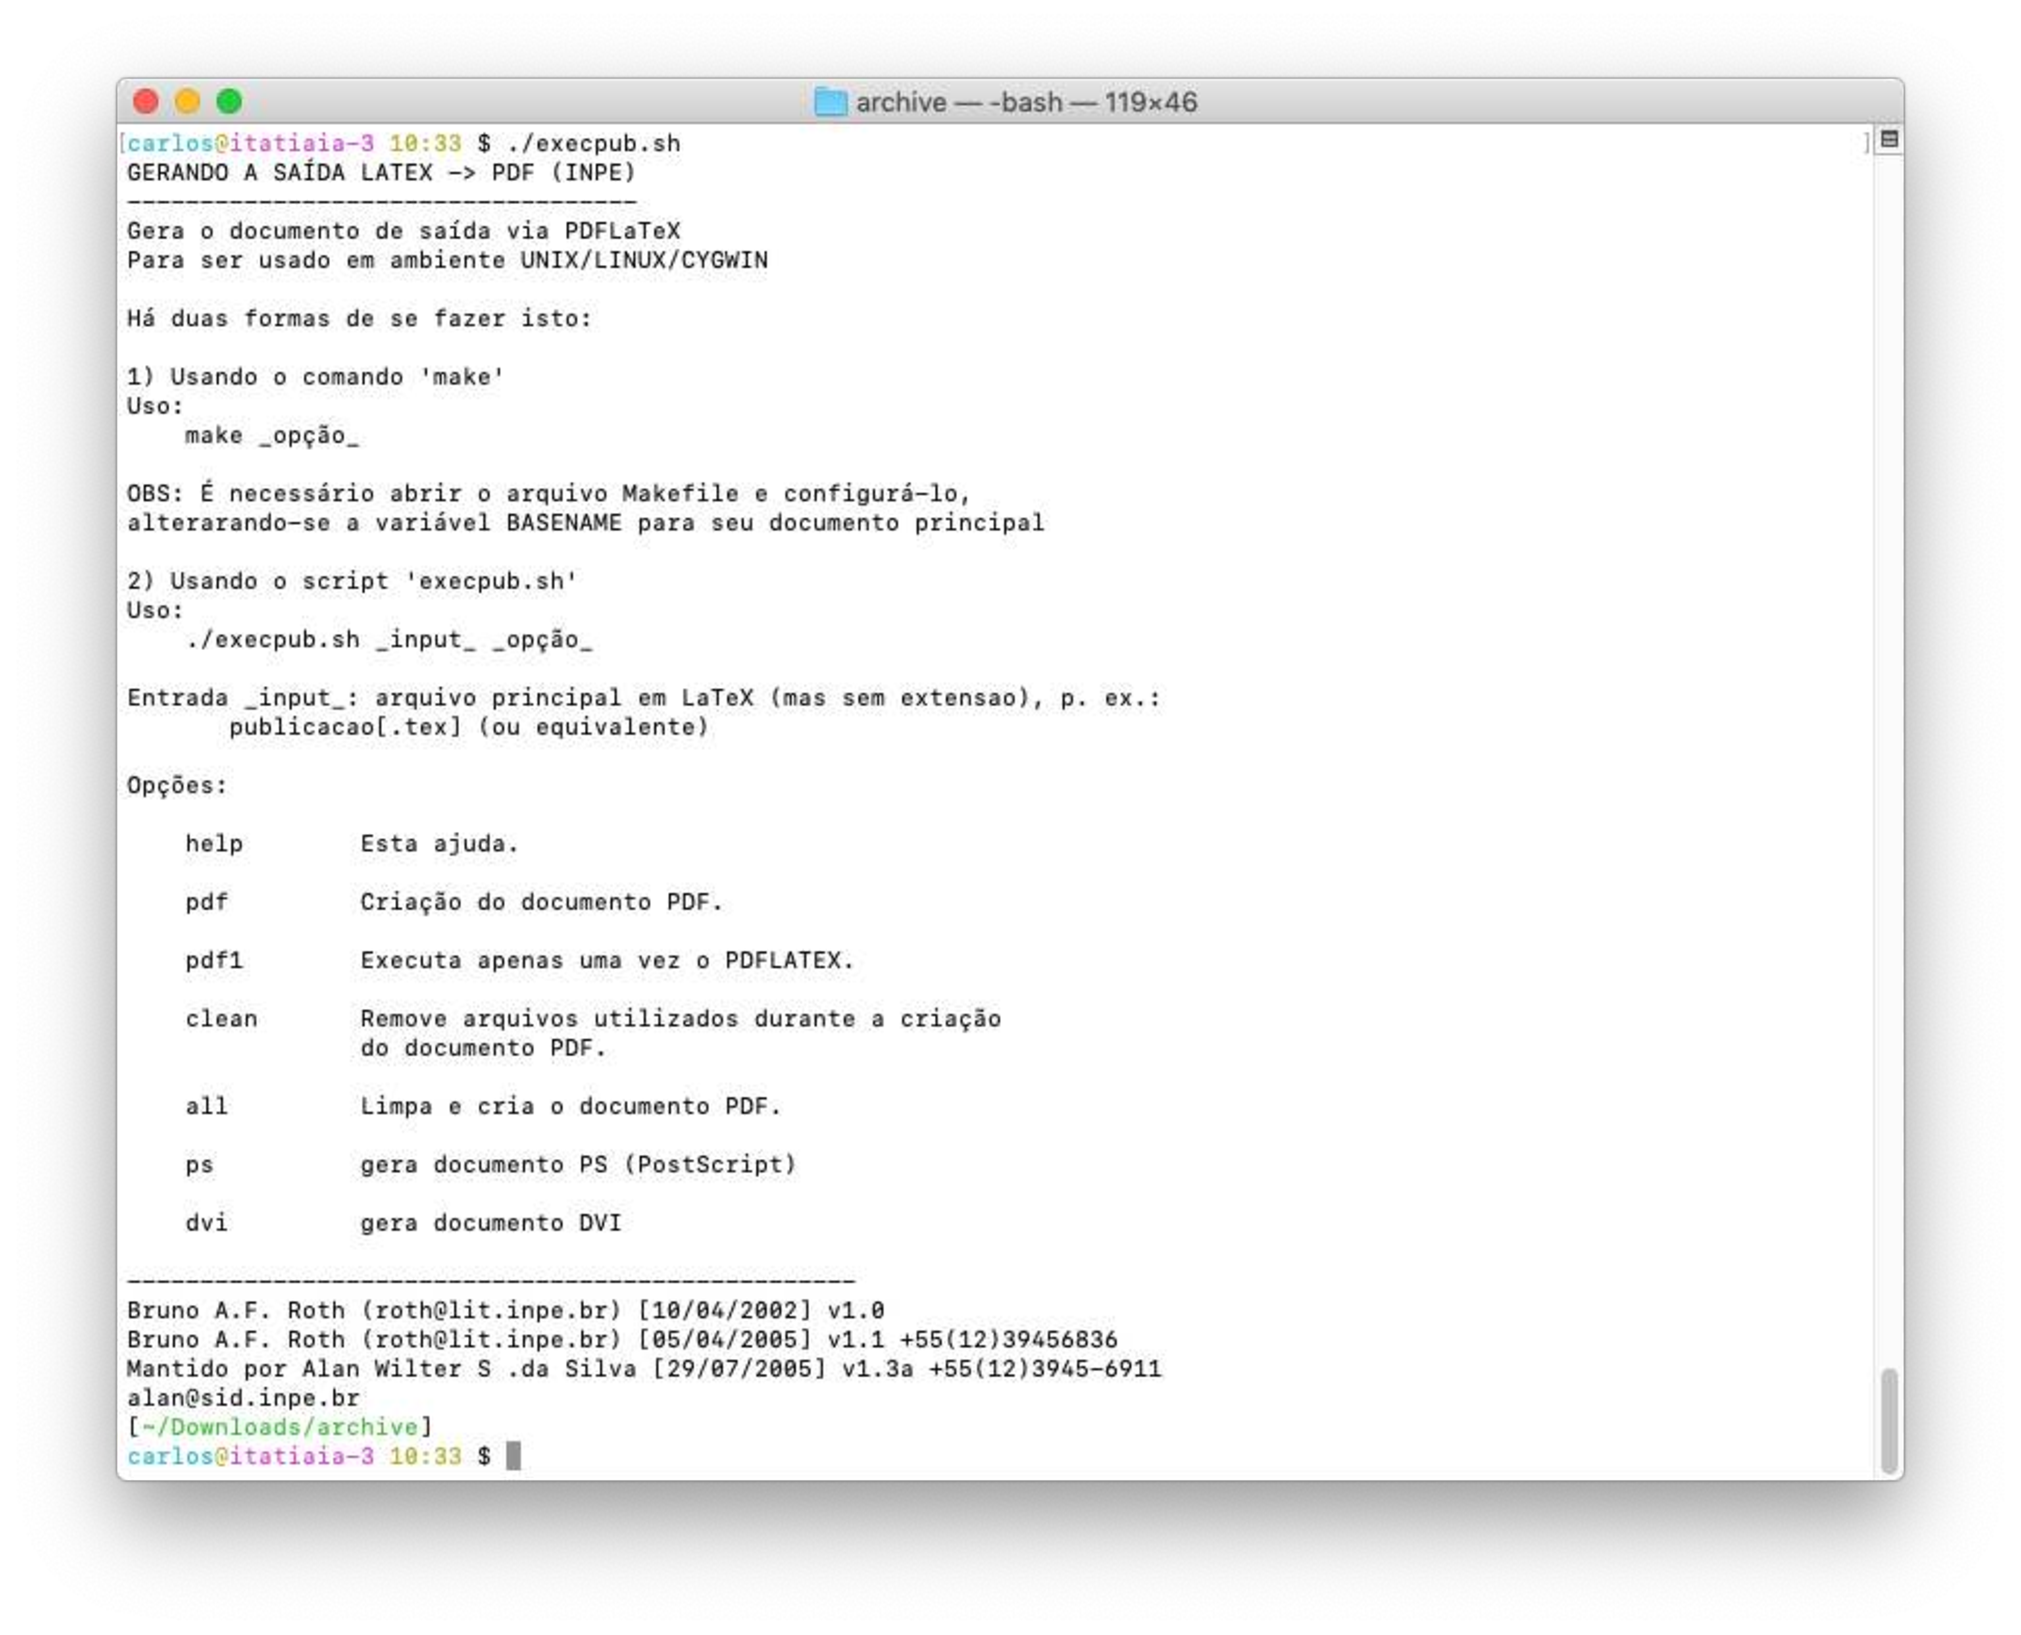
\includegraphics[scale=0.4]{./docs/figs/saida_execpub.pdf}
    \end{center}
\vspace{4mm}
\legenda{O \textit{script} {\tt execpub.sh}.}
\label{fig:execpub}
\FONTE{Produção do autor.}
\end{figure}

%\begin{commandshell}
%./execpub.sh
%GERANDO A SAÍDA LATEX -> PDF (INPE)
%-----------------------------------
%Gera o documento de saída via PDFLaTeX
%Para ser usado em ambiente UNIX/LINUX/CYGWIN
%
%Há duas formas de se fazer isto:
%
%1) Usando o comando 'make'
%Uso:
%    make _opção_
%
%OBS: É necessário abrir o arquivo Makefile e configurá-lo,
%alterarando-se a variável BASENAME para seu documento principal
%
%2) Usando o script 'execpub.sh'
%Uso:
%    ./execpub.sh _input_ _opção_
%
%Entrada _input_: arquivo principal em LaTeX (mas sem extensao), p. ex.:
%       publicacao[.tex] (ou equivalente)
%
%Opçõess:
%
%    help	Esta ajuda.
%
%    pdf		Criação do documento PDF.
%
%    pdf1	Executa apenas uma vez o PDFLATEX.
%
%    clean	Remove arquivos utilizados durante a criação
%		do documento PDF.
%
%    all		Limpa e cria o documento PDF.
%
%    ps	  	gera documento PS (PostScript)
%
%    dvi		gera documento DVI
%
%--------------------------------------------------
%Bruno A.F. Roth (roth@lit.inpe.br) [10/04/2002] v1.0
%Bruno A.F. Roth (roth@lit.inpe.br) [05/04/2005] v1.1 +55(12)39456836
%Mantido por Alan Wilter S .da Silva [29/07/2005] v1.3a +55(12)3945-6911
%alan@sid.inpe.br
%\end{commandshell}

\textbf{4.} Execute o \textit{script} {\tt execpub.sh}, com dois argumentos:
\begin{meucomando}
./execpub.sh <arquivo> <opcao>
\end{meucomando}

No comando acima, observe que o nome do arquivo a ser compilado deve ser informado sem a extensão {\tt .tex}.

Para finalmente compilar o documento principal {\tt publicacao.tex}, siga o exemplo abaixo. Observe que apenas este comando é necessário para gerar o arquivo PDF final ({\tt publicacao.pdf}).

\textbf{5.} Execute o \textit{script} {\tt execpub.sh}, com dois argumentos:
\begin{meucomando}
./execpub.sh publicacao pdf
\end{meucomando}

Muitos exemplos estão disponíveis na internet, assim como arquivos \LaTeX{} escritos há muito tempo e que podem fazer uso de codificações diferentes. Isso pode acarretar na representação incorreta de caracteres especiais, como acentos. Na Figura \ref{fig:leiame} o arquivo {\tt leiame} do estilo do INPE (assim como vários dos outros arquivos), foram criados e salvos na codificação ISO-8859-2 (frequentemente utilizado pelos sistemas operacionais até poucos anos atrás). Com a padronização do sistema \textit{Portable Operating System Interface} (POSIX) para UTF-8, pode tornar-se necessário abrir estes arquivos com algum editor de textos (como o Gedit no Linux ou o Textedit no MacOS) e utilizar a opção ``Salvar como...'' para salvar os arquivos no formato UTF-8. 

%\begin{figure}[H]
%\centering
%\subfigure[Renderização errada\label{fig:leiame1}]{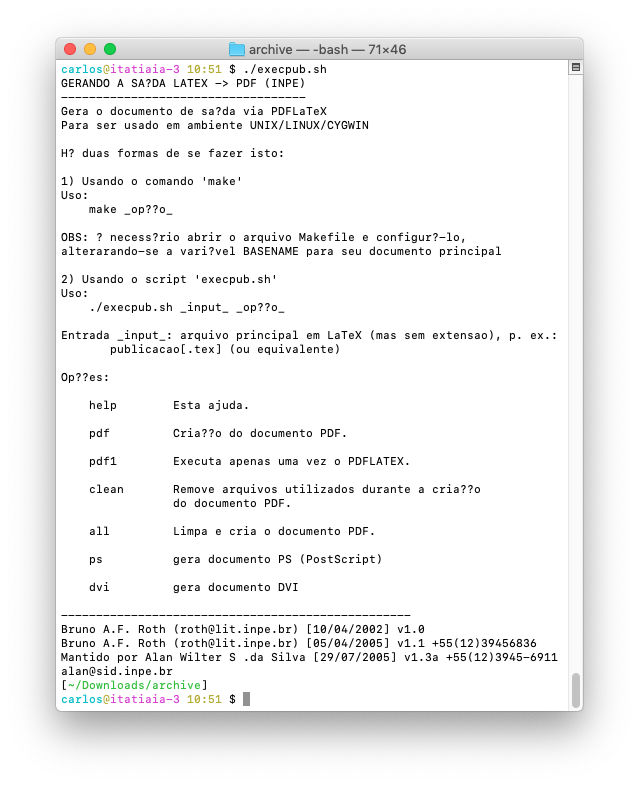
\includegraphics[scale=0.35]{./docs/figs/exemplo_iso8859_1.png}}%\\
%\subfigure[Renderização correta\label{fig:leiame2}]{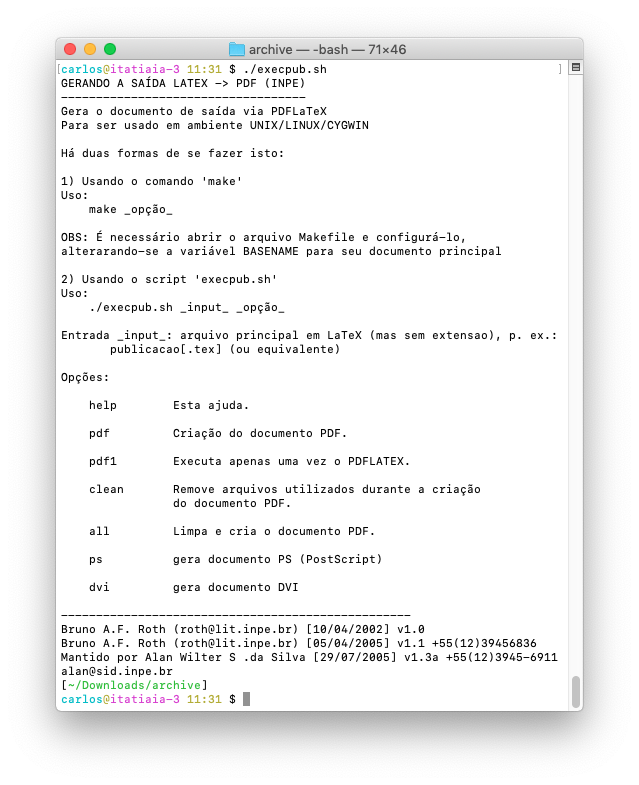
\includegraphics[scale=0.35]{./docs/figs/exemplo_iso8859_3.png}}
%\caption{Exemplo da renderização de um arquivo salvo com a codificação ISO-8859-2 em um ambiente UTF-8.}
%\label{fig:leiame}
%\end{figure}

\begin{figure}[H]
\caption{Exemplo da representação de um arquivo salvo com a codificação ISO-8859-2 em um ambiente UTF-8.}
\vspace{6mm}
    \begin{center}
    	%\label{fig:leiame1}
        \subfigure[Representação errada]{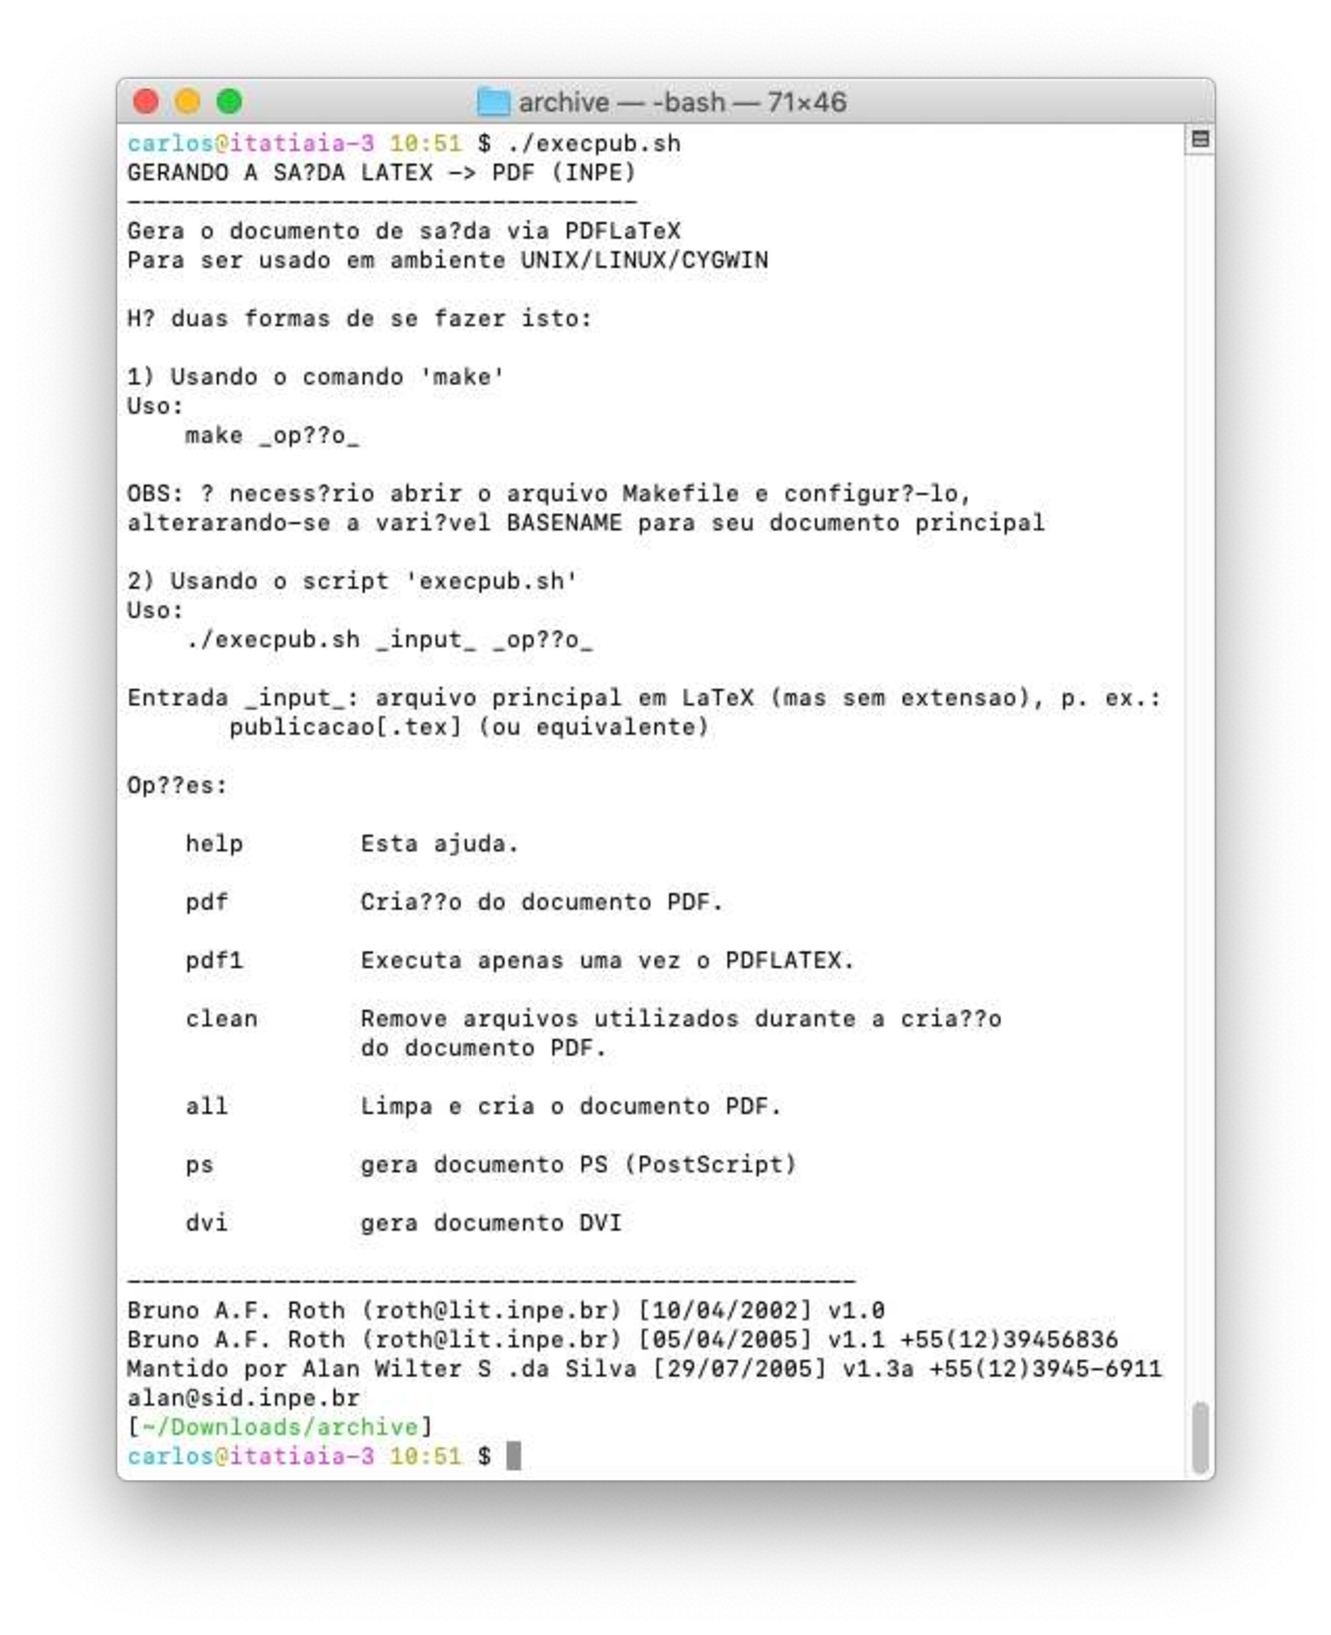
\includegraphics[scale=0.35]{./docs/figs/exemplo_iso8859_1.pdf}}%\\
		%\label{fig:leiame2}
		\subfigure[Representação correta]{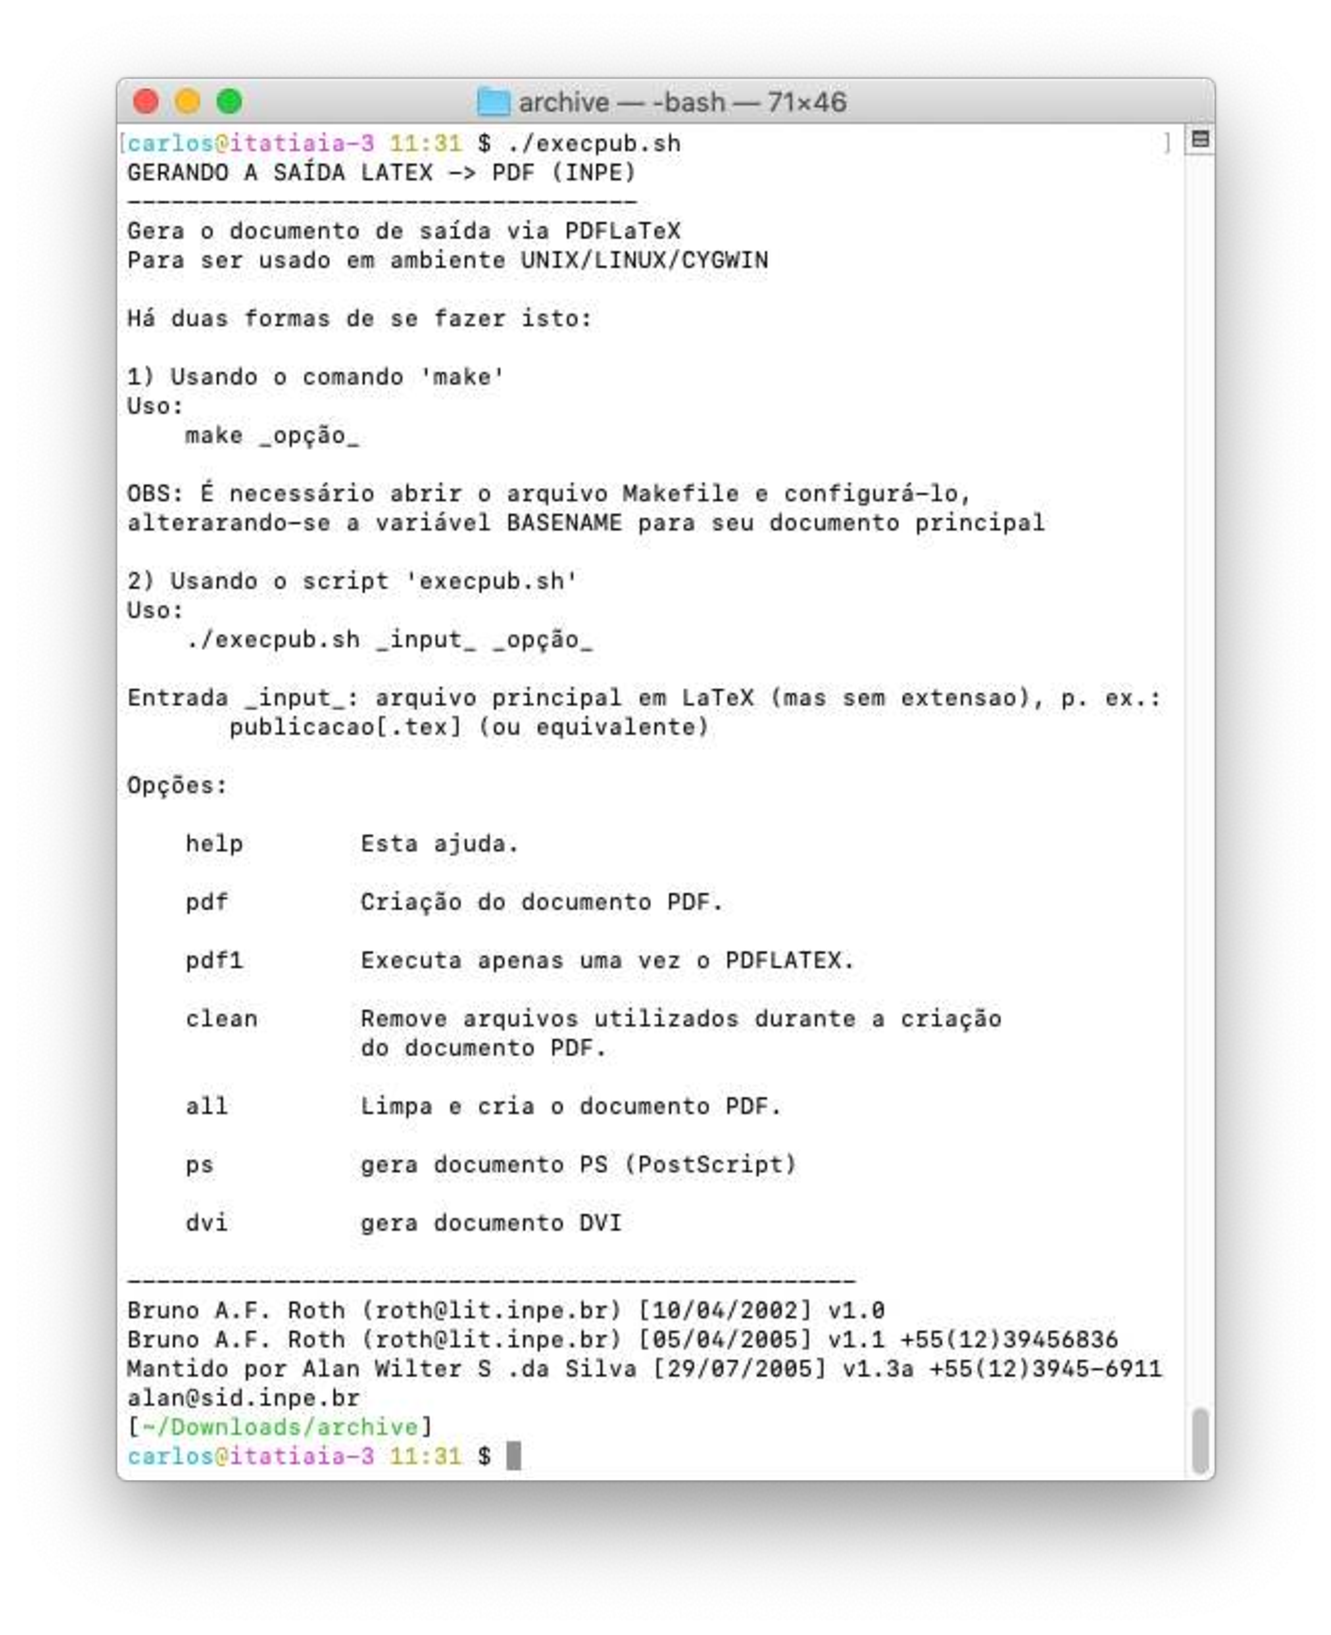
\includegraphics[scale=0.35]{./docs/figs/exemplo_iso8859_3.pdf}}
    \end{center}
\vspace{4mm}
\legenda{Exemplos das codificações ISO8859-2 e UTF-8.}
\label{fig:leiame}
\FONTE{Produção do autor.}
\end{figure}

%\begin{figure}[H]
%\centering
%\begin{subfigure}{.5\textwidth}
%  \centering
%  \includegraphics[scale=0.4]{./docs/figs/exemplo_iso88592_1.png}
%  \caption{A subfigure}
%  \label{fig:sub1}
%\end{subfigure}%
%\begin{subfigure}{.5\textwidth}
%  \centering
%  \includegraphics[scale=0.4]{./docs/figs/exemplo_iso88592_2.png}
%  \caption{A subfigure}
%  \label{fig:sub2}
%\end{subfigure}
%\caption{Exemplo da renderização de um arquivo salvo com a codificação ISO-8859-2 em um ambiente UTF-8.}
%\label{fig:leiame}
%\end{figure}
%
%\begin{figure}%
%    \centering
%    \subfloat[label 1]{{\includegraphics[width=5cm]{img1} }}%
%    \qquad
%    \subfloat[label 2]{{\includegraphics[width=5cm]{img2} }}%
%    \caption{2 Figures side by side}%
%    \label{fig:example}%
%\end{figure}

Outra forma de converter um arquivo ISO-8859-2 para o formato de codificação UTF-8, é através da utilização do comando {\tt iconv} do Linux (o qual também pode ser instalado no \textit{Microsoft Windows} através do SWL).Para converter um arquivo salvo na codificação ISO-8859-2 para UTF-8, pode-se utilizar o seguinte comando:

\begin{meucomando}
iconv -f ISO-8859-9 -t UTF-8 arquivo.tex > novo_arquivo.tex
\end{meucomando}

\begin{marker}
%Utilize o comando {\tt iconv} para converter arquivos salvos em codificações diferentes da UTF-8. Para converter um arquivo salvo na codificação ISO-8859-2 para UTF-8, pode-se utilizar o seguinte comando:
%\medskip
%\begin{meucomando}
%iconv -f ISO-8859-9 -t UTF-8 arquivo.tex > novo_arquivo.tex
%\end{meucomando}
%\medskip
Para mais informações sobre como utilizar o comando {\tt iconv}, digite o comando:
\smallskip
\begin{meucomando}
iconv --help
\end{meucomando}
\end{marker}

\subsection{Arquivos de Configuração}
\label{sec:configura}

No estilo do INPE, há basicamente dois arquivos que devem ser configurados para que o usuário possa definir o nome do(s) autor(es) e o título do documento. São eles: {\tt cofiguracao.tex} e {\tt publicacao.tex}.

%\begin{itemize}
%    \item {\tt publicacao.tex}
 %   \item {\tt configuracao.tex}
%\end{itemize}

No arquivo {\tt publicacao.tex}, são definidos o estilo da publicação, i.e., se o documento terá o estilo de dissertação ou tese ({\tt PublicacaoDissOuTese}, é o padrão), artigo ou relatório ({\tt PublicacaoArtigoOuRelatorio}), proposta de tese ou dissertação ({\tt PublicacaoProposta}), livro com ou sem a formatação de capítulos ({\tt PublicacaoLivro}). Além disso, deve-se ajustar também o idioma: se o idioma principal do documento for o Português, então o \textit{abstract} será no idioma Inglês ({\tt english, portuguese}), além do tipo de logo do governo e do tipo de licença \textit{Creative Commons} (CC) a ser utilizada (veja mais informações sobre os diferentes tipos de Licenças \textit{Creative Commons} em \url{https://pt.wikipedia.org/wiki/Licenças_Creative_Commons}). Veja no exerto a seguir, um trecho do arquivo {\tt publicacao.tex}.

%\begin{torntext}[title=Trecho do arquivo {\tt publicacao.tex}]
%$\backslash$\mintinline{latex}{documentclass[\%}
%\\
%\%\%\% PARA ESCOLHER O ESTILO TIRE O SIMBOLO \%(COMENTÁRIO)
%\\
%\%SemVinculoColorido,
%\\
%\%SemFormatacaoCapitulo,
%\\
%\%SemFolhaAprovacao,
%\\
%\%SemImagens,
%\\
%\%CitacaoNumerica, \%\% o padrão é citação tipo autor-data
%\\
%\%PublicacaoDissOuTese, \%\% (é também o "default") com ficha catal. e folha de aprovação em branco. Caso tenha lista de símbolos e lista de siglas e abreviaturas retirar os comentários dos arquivos siglas.tex e abreviaturasesiglas.tex. Retirar também os comentários indicados nesse arquivo, nos includes
%\\
%\%PublicacaoArtigoOuRelatorio, \%\% texto sequencial, sem quebra de páginas nem folhas em branco
%\\
%\%PublicacaoProposta, \%\% igual tese/dissertação, mas sem ficha catal. e fol. de aprov.
%\\
%\%PublicacaoLivro, \%\% com capítulos
%\\
%\%PublicacaoLivro,SemFormatacaoCapitulo, \%\% sem capítulos
%\\
%english,portuguese \%\% para os documentos em Português com abstract.tex em Inglês
%\\
%\%portuguese,english \%\% para os documentos em Inglês com abstract.tex em Português
%\\
%,LogoINPE\% comentar essa linha para fazer aparecer o logo do Governo
%\\
%,CCBYNC	\% as opções de licença são: CCBY, CCBYSA, CCBYND, CCBYNC, CCBYNCSA, CCBYNCND, GPLv3 e INPECopyright
%\\
%]{tdiinpe}
%\\
%\%]{../../../../../iconet.com.br/banon/2008/03.25.01.19/doc/tdiinpe}
%\\
%\% PARA EXIBIR EM ARIAL TIRAR O COMENTÁRIO DAS DUAS LINHAS SEGUINTES
%\\
%\%$\backslash$\mintinline{latex}{renewcommand{\rmdefault}{phv}} \% Arial
%\\
%\%$\backslash$\mintinline{latex}{renewcommand{\sfdefault}{phv}} \% Arial
%\\
%\\
%\% PARA PUBLICAÇÕES EM INGLÊS:
%\\
%\% renomear o arquivo: abnt-alf.bst para abnt-alfportuguese.bst
%\\
%\% renomear o arquivo: abnt-alfenglish.bst para abnt-alf.bst
%\end{torntext}

%\begin{tcboxedraster}[raster columns=3, raster equal height, size=small,colframe=red!50!black,colback=red!10!white,colbacktitle=red!50!white, title={Box \# \thetcbrasternum}] {colback=yellow!10,fonttitle=\bfseries,title=Trecho do arquivo {\tt publicacao.tex}}
%$\backslash$\mintinline{latex}{documentclass[\%}
%\\
%\%\%\% PARA ESCOLHER O ESTILO TIRE O SIMBOLO \%(COMENTÁRIO)
%\\
%\%SemVinculoColorido,
%\\
%\%SemFormatacaoCapitulo,
%\\
%\%SemFolhaAprovacao,
%\\
%\%SemImagens,
%\\
%\%CitacaoNumerica, \%\% o padrão é citação tipo autor-data
%\\
%\%PublicacaoDissOuTese, \%\% (é também o "default") com ficha catal. e folha de aprovação em branco. Caso tenha lista de símbolos e lista de siglas e abreviaturas retirar os comentários dos arquivos siglas.tex e abreviaturasesiglas.tex. Retirar também os comentários indicados nesse arquivo, nos includes
%\\
%\%PublicacaoArtigoOuRelatorio, \%\% texto sequencial, sem quebra de páginas nem folhas em branco
%\\
%\%PublicacaoProposta, \%\% igual tese/dissertação, mas sem ficha catal. e fol. de aprov.
%\\
%\%PublicacaoLivro, \%\% com capítulos
%\\
%\%PublicacaoLivro,SemFormatacaoCapitulo, \%\% sem capítulos
%\\
%english,portuguese \%\% para os documentos em Português com abstract.tex em Inglês
%\\
%\%portuguese,english \%\% para os documentos em Inglês com abstract.tex em Português
%\\
%,LogoINPE\% comentar essa linha para fazer aparecer o logo do Governo
%\\
%,CCBYNC	\% as opções de licença são: CCBY, CCBYSA, CCBYND, CCBYNC, CCBYNCSA, CCBYNCND, GPLv3 e INPECopyright
%\\
%]{tdiinpe}
%\\
%\%]{../../../../../iconet.com.br/banon/2008/03.25.01.19/doc/tdiinpe}
%\\
%\% PARA EXIBIR EM ARIAL TIRAR O COMENTÁRIO DAS DUAS LINHAS SEGUINTES
%\\
%\%$\backslash$\mintinline{latex}{renewcommand{\rmdefault}{phv}} \% Arial
%\\
%\%$\backslash$\mintinline{latex}{renewcommand{\sfdefault}{phv}} \% Arial
%\\
%\\
%\% PARA PUBLICAÇÕES EM INGLÊS:
%\\
%\% renomear o arquivo: abnt-alf.bst para abnt-alfportuguese.bst
%\\
%\% renomear o arquivo: abnt-alfenglish.bst para abnt-alf.bst
%\end{tcboxedraster}

\begin{texexp}{listing only}
documentclass[
% PARA ESCOLHER O ESTILO TIRE O SIMBOLO (COMENTÁRIO)
%SemVinculoColorido,
%SemFormatacaoCapitulo,
%SemFolhaAprovacao,
%SemImagens,
%CitacaoNumerica, 
%PublicacaoDissOuTese,
%PublicacaoArtigoOuRelatorio,
%PublicacaoProposta, 
%PublicacaoLivro, 
%PublicacaoLivro,SemFormatacaoCapitulo,
english,portuguese, 
%portuguese,english, 
LogoINPE,
CCBYNC,
]{tdiinpe}

% PARA EXIBIR EM ARIAL TIRAR O COMENTÁRIO DAS DUAS LINHAS SEGUINTES
%\renewcommand{\rmdefault}{phv}} % Arial
%\renewcommand{\sfdefault}{phv}} % Arial

% PARA PUBLICAÇÕES EM INGLÊS:
%renomear o arquivo: abnt-alf.bst para abnt-alfportuguese.bst
%renomear o arquivo: abnt-alfenglish.bst para abnt-alf.bst
...
\end{texexp}

A Tabela \ref{tab:arq_publicacao} sumariza as principais opções encontradas no arquivo {\tt publicacao.tex}.

\begin{table}[H]
\centering
\caption{Configurações principais do arquivo {\tt publicacao.tex}.}
\label{tab:arq_publicacao}
    \begin{tabular}{p{6.5cm}p{6.5cm}}
    \toprule
    \textbf{Opção} & \textbf{Descrição} \\
    \midrule
    {\tt SemVinculoColorido}                    & Remove o realce das referências e \textit{links} \\
    {\tt SemFormatacaoCapitulo}                 & Não aplica a formatação de capítulos  \\
    {\tt SemImagens}                            & Compila o documento sem as imagens\footnotemark[1] \\
    {\tt CitacaoNumerica}                       & Altera o estilo das citações \\
    {\tt PublicacaoDissOuTese}                  & Aplica o estilo de Dissertação ou Tese \\
    {\tt PublicacaoArtigoOuRelatorio}           & Aplica o estilo de Artigo ou Relatório \\
    {\tt PublicacaoProposta}                    & Aplica o estilo de Proposta (Tese ou Dissertação) \\
    {\tt PublicacaoLivro}                       & Aplica o estilo de Livro \\
    {\tt PublicacaoLivro},\newline{\tt SemFormatacaoCapitulo} & Idem anterior, mas sem a formatação de capítulos \\
    {\tt english,portuguese}                    & Texto em Português, \textit{Abstract} em Inglês \\
    {\tt portuguese,english}                    & Texto em Inglês, Resumo em Português \\
    {\tt LogoINPE}                              & Utiliza o logo do INPE ao invés do logo do governo \\
    {\tt CCBYNC}                                & Aplica o tipo de licença \\
    \mintinline{latex}{\renewcommand{\rmdefault}{phv}}& Aplica a fonte Arial (sem serifa) como padrão \\
%    \\[-0.5em]
%    {\tt LogoINPE}                              & Utiliza o logo do INPE ao invés do logo do governo \\
%    \\[-0.5em]
%    {\tt LogoINPE}                              & Utiliza o logo do INPE ao invés do logo do governo \\
%    \\[-0.5em]
    \bottomrule
    \end{tabular}
\FONTE{Produção do autor.}
\end{table}

\footnotetext[1]{Esta opção pode ser útil quando se tem muitas imagens e o tempo de compilação do documento for muito grande.}

%\begin{leaflet}[underlay={\node[above=5mm,font=\footnotesize] 
%    at (frame.south) {- \arabic{tcbbreakpart} -};}]
%     \includegraphics[width=\linewidth]{Basilica_5.png}
%     \begin{center}
%     \bfseries\LARGE Example
%     \end{center}
%     \section{Introduction}
%     \lipsum[1]
%     \section{Main Part A}
%     \lipsum[2-8]
%     \section{Main Part B}
%     \lipsum[9-15]
%     \section{Conclusion}
%     \lipsum[16-18]
%\end{leaflet}

No arquivo {\tt configuracao.tex}, o usuário poderá inserir o título do documento, bem como o(s) nome(s) do(s) autor(es) do documento. Outras configurações, são normalmente revisadas e alteradas oportunamente pelo SESID quando o documento de tese ou dissertação é entregue para revisão do estilo.

\begin{texexp}{listing only}
% CAPA
\titulo{Escrever o t\'{i}tulo no idioma em que foi escrito a
publicaç\~{a}o}
\title{Escrever o t\'{i}tulo em Ingl\^{e}s para publicaç\~{o}es
escritas em Portugu\^{e}s e em Portugu\^{e}s para publicaç\~{o}es
escritas em Ingl\^{e}s} 
\author{Nome Completo do Autor}
\descriccao{Tese de Doutorado ou Dissertaç\~{a}o de Mestrado do
Curso de P\'{o}s-Graduaç\~{a}o em Nome do Curso, orientada pelo(a)
Dr(a). Nome do Orientador(a), aprovada em dd de m\^{e}s por extenso
de aaaa.}
\repositorio{aa/bb/cc/dd}
\tipoDaPublicacao{TDI}
\IBI{xx/yy} 
\date{AAAA}
...
\end{texexp}

\begin{marker}
Recomenda-se atenção especial para os caracteres que são inseridos no arquivo {\tt configuracao.tex}. Neste arquivo, os acentos devem ser marcados, e.g., a palavra ``{\tt publicação}'', deve ser marcada como ``\mintinline{latex}{publicaç\~{a}o}.''
\end{marker}

%\subsection{Estrutura dos diretórios e arquivos de configuração}
%\subsection{Inclusão de pacotes e suas funções}
%\subsection{Como são divididas as seções}
%\subsection{Introduzindo figuras e gráficos}
%\subsection{Inserindo tabelas e equações}
%\subsection{Citações, Referências Cruzadas e Referências (bibtex, abntex)}
%
%\section{Utilização de Editores}
%\subsection{Linha de comando, editores locais, editor online (Overleaf)}
%
%\section{Ferramentas Úteis}
%\subsection{Construção de tabelas}
%\subsection{Gerenciadores de referências (Mendeley, Zotero)}

As seções a seguir são dedicadas aos detalhes referentes à inserção de conteúdo nos documentos que farão uso do estilo do INPE.

\subsection{Inserção de Figuras e Tabelas}
\label{sec:figtabs}

Na Seção \ref{sec:figuras} do Capítulo \ref{cap:parteII} foram apresentadas diferentes formas de se incluir figuras em um documento \LaTeX{}. Com a utilização do estilo do INPE, entretanto, alguns cuidados deverão ser tomados, pois há alguns detalhes que devem ser respeitados. Uma imagem típica com todos os seus elementos de referência é apresentada no Exemplo \ref{figestinpe}.

\begin{texexptitled}[breakable,center lower,enhanced,middle=2mm,listing and text]{Inserção de uma figura utilizando o estilo do INPE}{figestinpe}
\begin{figure}[H]
  \caption{Exemplo de figura com título curto.}
  \vspace{6mm} % acrescentar o espaçamento vertical apropriado entre o título e a borda superior da figura
  \begin{center}
    \includegraphics[width=12cm]{./docs/figs/gpa.pdf}  
  \end{center}
  \vspace{4mm} % acrescentar o espaçamento vertical apropriado entre a borda inferior da figura e a legenda ou a fonte quando não há legenda (o valor pode ser negativo para subir)
  \legenda{Exemplo de legenda curta.} % legenda - opcional
  \label{figgpa1}
  \FONTE{\citeonline{lba/06}.} % fonte consultada (elemento obrigatório, mesmo que seja produção do próprio autor)
\end{figure}
\end{texexptitled}

No Exemplo \ref{figestinpe}, observe que espaçamentos especiais são aplicados utilizando-se os comandos {\tt vspace} que aplicam um espaçamento de {\tt 6mm} entre o \textit{caption} (que fica em cima da figura) da figura e um espaçamento de {\tt 4mm} entre a figura e a legenda (que fica embaixo da figura). Esta segunda legenda é opcional e geralmente se constitui de uma frase curta sobre a imagem mostrada. Um elemento obrigatório é a incorporação do marcador {\tt FONTE} (em caixa alta), o qual deve conter a fonte consultada ou, se a produção for do autor, deve conter a frase ``Produção do autor''. Para mais exemplos de inserção de figuras de estilos diferentes, verifique o Anexo B de \citeonline{estiloinpe}.

Tabelas também devem seguir a formatação estipulada pelo estilo do INPE. Veja o Exemplo \ref{tabestinpe} a seguir.

\begin{texexptitled}[breakable,center lower,enhanced,middle=2mm,listing and text]{Inserção de uma tabela utilizando o estilo do INPE}{tabestinpe}
\begin{table}[H] % [htbp] opções de posicionamento da tabela no texto
\begin{center} % use sempre um ambiente para as tabelas
% (opções: center (recomendado), flushright, flushleft)
% NÃO USE \centering com TABELAS se houver \FONTE!	
\caption{Exemplo de tabela, com fonte.}
\begin{tabular}{l|l|c|c|r|r}
\hline % desenha uma linha horizontal
Campo 1 & Campo2 & Campo3 & Campo 4 & Campo5 & Campo6 \\
Campo 1 & Campo2 & Campo3 & Campo 4 & Campo5 & Campo6 \\
Campo 1 & Campo2 & Campo3 & Campo 4 & Campo5 & Campo6 \\				
\hline % desenha uma linha horizontal
\end{tabular}
\end{center}
\FONTE{Coloque a fonte de referência aqui, se houver.}
\end{table}
\end{texexptitled}

No caso das tabelas, sempre que se utilizar o estilo do INPE, deve-se utilizar o ambiente {\tt table} (veja mais detalhes na Seção \ref{sec:tabs} do Capítulo \ref{cap:parteII}). Recomenda-se também a utilização dos ambientes de posição (para centralizar, alinhar à direita ou esquerda). Da mesma forma como as figuras, as tabelas também devem vir acompanhadas do marcador {\tt FONTE}, sempre que a citação da fonte for permitente. Neste caso, evite a utilização do marcado {\tt centering} e passe a utilizar o ambiente {\tt center}. Mais detalhes sobre a inserção de tabelas utilizando-se o estilo do INPE, podem ser encontradas no Anexo B de \citeonline{estiloinpe}.

Tanto para figuras quanto para tabelas, o posicionamento destes corpos flutuantes é importante. Os ambientes {\tt figure} e {\tt table}, devem ter suas posições relativas ajustadas conforme as opções mostradas na Tabela \ref{tab:ambfig} da Seção \ref{sec:amb_docs/figs} do Capítulo \ref{cap:parteII}.

\subsection{Inserção de Citações e Referências}
\label{sec:citerefs}

Assim como apresentado na Seção \ref{sec:refs} do Capítulo \ref{cap:parteII}, citações a elementos do texto como figuras, tabelas e equações podem ser feitas com a utilização do par de comandos {\tt label} e {\tt ref}. Referências bibliográficas, dentro do estilo do INPE, são gerenciadas utilizando o Bib\TeX{} e a sua inserção em um documento com o estilo do INPE, é simples. Antes de apresentar os detalhes de como as referências são armazenadas e incluídas no corpo do texto, é necessário antes, voltar à Seção \ref{sec:compilacao} do Capítulo \ref{cap:parteII} e acrescentar alguns passos extras ao processo de compilação. Isso se faz necessário porque as referências bibliográficas precisam também ser interpretadas pelo Bib\TeX{}. Nesse processo, o estilo de referências da ABNT é então aplicado e apresentado da forma correta no corpo do texto.

Na Figura \ref{fig:compbibtex} é apresentado um diagrama semelhante aquela apresentada na Figura \ref{fig:complatex}, com a diferença de que os procedimentos necessários para a inclusão do Bib\TeX{} estão adicionados.

\begin{figure}[H]
	\caption{Etapas envolvidas na compilação de um documento \LaTeX{} com referências Bib\TeX{}.}
	\vspace{6mm}
	\begin{center}
		\includegraphics[scale=0.6,angle=-90,trim={4.5cm 1cm 6cm 1cm},clip]{./docs/figs/diagramacompbib.pdf}
	\end{center}
	\vspace{4mm}
	\legenda{Compilação de um documento \LaTeX{}.}
	\label{fig:compbibtex}
	\FONTE{Adaptado de \url{http://www.texample.net/tikz/examples/tex-workflow/}.}
\end{figure}

O processo de compilação de um documento \LaTeX{} com referências Bib\TeX{}, inclui a utilização do programa {\tt bibtex}. Em sequência, uma compilação manual completa (i.e., gerando o arquivo PDF no final), tem a seguinte ordem:

\begin{meucomando}
latex documento.tex
bibtex documento
latex documento
latex documento
dvips documento.dvi
ps2pdf documento.ps
\end{meucomando}

Na sequência de comandos acima, observe que foram utilizados o comando {\tt latex documento} duas vezes seguida após o comando {\tt bibtex documento}. Isso se faz necessário porque o Bib\TeX{} processa as informações de referências e escreve algumas informações em disco, em arquivos auxiliares. Depois, o \LaTeX{} lê esta informação e formata as referências, que são incorporadas finalmente ao documento, apenas após a segunda vez em que o comando é executado.

No estilo do INPE, existe um arquivo de nome {\tt referencia.bib} que fica dentro do diretório {\tt bib/}. Este arquivo possui uma estrutura específica e tem o seguinte aspecto:

\begin{texexp}{listing only}
%% NOTA: em vez de usar as letras e vogais com acento ou sinais gr\'aficos (como o c cedilhado -- \c c), algo normal agora no texto em LaTeX, use aqui suas formas no padrão LaTeX, p. ex.:
%% \'a = a agudo (mesmo para outras vogais)
%% \^a = a circunflexo  
%% \`a = a craseado
%% \"a = a tremado
%% {\c c} = c cedilhado
%% Isto ainda é necessário para evitar inconsistências na geração da lista de referências bibliográficas.

@string{cs =      "Complex Systems"}
@string{pl =      "Physics Letters"}
@string{prl =     "Physical Review Letters"}
@string{pra =     "Physical Review A"} 
@string{pla =     "Physics Letters A"} 
@string{pre =     "Physical Review E"} 
@string{pd =      "Physica D"} 
@string{jcsc =    "Journal of Circuits, Systems and Computers"}
@string{jsv =     "Journal of Sound and Vibration"}
@string{ijbc =    "International Journal of Bifurcation and Chaos"}
@string{ijc =     "International Journal of Control"}
@string{ieeecas = "IEEE Transactions on Circuits and Systems"}
@string{jrssb =   "Journal of the Royal Statistical Society B"} 
@string{n =       "Nature"}
@string{zn =      "Z. Naturforsch"}
@string{jfi =     "Zeitschrift fuer Naturforschung A"} 
@string{actaam =  "ACTA Amaz\^onica"}

@ARTICLE{nobre/2005,
  author    = {Luizao, F. J. and Nobre, C. A. and Manzi, A. O.},
  title     = {Projeto LBA: Estudando as Complexas Intera{\c c}\~oes da Biosfera com a Atmosfera na Amaz\^onia},
  journal   = actaam,
  year      = {2005},
  volume    = {35},
  number    = {1-2},
  pages     = {109--110},
}
...
\end{texexp}

Neste arquivo, observe que está indicado em um comentário no topo do arquivo, que o usuário insira os acentos de forma explícita, tal como foi explicado na Seção \ref{sec:acentos} do Capítulo \ref{cap:parteII}. Isto se faz necessário porque o Bib\TeX{} não aceita a localização tal como pode-se fazer com o \LaTeX{} quando se utiliza o pacote {\tt inputenc}. No segundo bloco, observe as instruções que se iniciam com a palavra-chave {\tt @string}. Com estas \textit{strings} pode-se criar atalhos (\textit{aliases}) para nomes que podem ser expandidos depois na montagem das referências, feitas pelo Bib\TeX{}. Repare que a \textit{string} que define o \textit{alias} {\tt actaam} foi utilizado no campo {\tt journal} da referência de \citeonline{nobre/2005}. O arquivo {\tt referencia.bib} pode se tornar muito grande. Neste caso, pode ser interessante utilizar algum gerenciador de referências, tal como o \textit{Zotero}, \textit{Mendeley}, \textit{Jabref} entre outros (veja algumas destas opções na Seção \ref{sec:refs} do Capítulo \ref{cap:parteII}). 

\begin{marker}
Deve-se ter cautela na edição manual do arquivo {\tt referencia.bib} do estilo do INPE. Este arquivo não aceita acentos naturais, i.e., acentos latinos devem ser marcados no estilo do \LaTeX{} (veja mais detalhes na Seção \ref{sec:acentos}. Além disso, é recomendável que o usuário edite a referência, removendo espaços em brancos e remarcando os acentos, quando necessário.
\end{marker}

As referências bibliográficas, dentro da norma ABNT adotada pelo estilo do INPE, podem ser inseridas no corpo do texto com os marcadores sumarizados na Tabela \ref{tab:estiloscit}. As definições destes marcadores podem ser encontradas em \citeonline{araujo/2018} e também no arquivo {\tt abntcite.sty} do estilo do INPE.

Na Tabela \ref{tab:estiloscit} a seguir, as duas referências utilizadas nos exemplos são as seguintes:

\begin{texexp}{listing only}
@article{fulano/1964,
  author = {Fulano, Sicrano},
  title = {Um Exemplo de Refer{\^e}ncia Bibliogr{\'a}fica do tipo article.},
  journal = {Revista Mensal de Ci{\^e}ncia},
  volume = {12},
  number = {11},
  pages = {340-346},
  year = {1964},
}

@article{ciclanoetal/1975,
  author = {Ciclano, Beltrano and Fulano, Sicrano},
  title = {Mais um exemplo de Refer{\^e}ncia Bibliogr{\'a}fica do tipo article.},
  journal = {Revista Mensal de Ci{\^e}ncia},
  volume = {2},
  number = {21},
  pages = {430-436},
  year = {1975},
}
\end{texexp}

\newpage

\begin{landscape}

\vfill

\begin{table}[htb]
\centering
\caption{Estilos de citação segundo as normas ABNT no estilo do INPE.}
\label{tab:estiloscit}
\begin{tabular}{p{3.5cm} p{11cm} p{7cm}}
	\toprule
	\textbf{Opção}         & \textbf{Uso}                                                            & \textbf{Exemplo}                                    \\
	\midrule                                                                                                                                    
	{\tt cite}             & \mintinline{latex}{\cite{fulano/1964}}                                  & \cite{fulano/1964}                                  \\
	{\tt citeonline}       & \mintinline{latex}{\citeonline{fulano/1964}}                            & \citeonline{fulano/1964}                            \\
	{\tt citeyear}         & \mintinline{latex}{\citeyear{fulano/1964}}                              & \citeyear{fulano/1964}                              \\
	{\tt citeauthor}       & \mintinline{latex}{\citeauthor{ciclanoetal/1975}}                       & \citeauthor{ciclanoetal/1975}                            \\
	{\tt citeauthoronline} & \mintinline{latex}{\citeauthoronline{fulano/1964}}                      & \citeauthoronline{fulano/1964}                      \\
    \midrule
	{\tt apud}             & \mintinline{latex}{\apud[p.~2--3]{fulano/1964}{ciclanoetal/1975}}       & \apud[p.~2--3]{fulano/1964}{ciclanoetal/1975}       \\
	{\tt apudonline}       & \mintinline{latex}{\apudonline[p.~2--3]{fulano/1964}{ciclanoetal/1975}} & \apudonline[p.~2--3]{fulano/1964}{ciclanoetal/1975} \\
	{\tt Idem}             & \mintinline{latex}{\Idem[p.~2--3]{ciclanoetal/1975}}                    & \Idem[p.~2--3]{ciclanoetal/1975}                    \\
	{\tt Ibidem}           & \mintinline{latex}{\Ibidem[p.~2--3]{ciclanoetal/1975}}                  & \Ibidem[p.~2--3]{ciclanoetal/1975}                  \\
	{\tt opcit}            & \mintinline{latex}{\opcit[p.~2--3]{ciclanoetal/1975}}                   & \opcit[p.~2--3]{ciclanoetal/1975}                   \\
	{\tt passim}           & \mintinline{latex}{\passim{ciclanoetal/1975}}                           & \passim{ciclanoetal/1975}                           \\
	{\tt loccit}           & \mintinline{latex}{\loccit{ciclanoetal/1975}}                           & \loccit{ciclanoetal/1975}                          \\
	{\tt cfcite}           & \mintinline{latex}{\cfcite[p.~2--3]{ciclanoetal/1975}}                  & \cfcite[p.~2--3]{ciclanoetal/1975}                  \\
	{\tt etseq}            & \mintinline{latex}{\etseq{fulano/1964}}                                 & \etseq{fulano/1964}                                 \\
	\bottomrule                                                                                                                                     
\end{tabular}
\FONTE{Produção do autor.}
\end{table}

\end{landscape}

\vfill
\clearpage
\newpage

A aplicação dos estilos mostrados na Tabela \ref{tab:estiloscit}, deve ser feita em ocasiões específicas. Os marcadores {\tt cite} e {\tt citeonline} são mais frequentemente utilizados, mas observe que dependendo do estilo de escrita do autor, pode ser necessário apenas citar-se ou o ano (com o marcador {\tt citeyear}), ou apenas o autor (com os marcadores {\tt citeauthor} ou {\tt citeauthoronline}). Os marcadores {\tt apud} e {\tt apudonline} devem ser utilizados para citar referências que são encontradas em outras referências. Neste caso, a utilização do \textit{apud} (uma expressão latina que indica uma intermediação) pode não ser muito elegante, pois pode passar a impressão de que o autor não leu ou não teve acesso à referência original. Citações com os marcadores {\tt Idem} e {\tt Ibidem} indicam, respectivamente, ``mesmo autor'' e ``mesma obra'', e seu uso parece ser mais claro. O marcador {\tt opcit}, representa a expressão latina \textit{opus citatum}, que significa ``obra citada'', ao passo que o marcador {\tt cfcite}, representa a expressão latina \textit{confira}, o marcador {\tt passim}, representa a expressão latina \textit{passim}, equivalente a ``aqui e ali'', enquanto que o marcador {\tt etseq} representa a expressão latina \textit{et sequentia}, equivalente a ``e sequência''.

De forma geral, as referências em um documento \LaTeX{} escrito com o estilo do INPE, devem seguir as mesmas orientações indicadas na Seção \ref{sec:citerefs} do Capítulo \ref{cap:parteII}. Para mais informações sobre a elaboração de referências bibliográficas seguindo as normas ABNT, consulte \citeonline{barbedo/2018a,barbedo/2018b}.

\subsection{Orientações Especiais}
\label{sec:oriesp}

O estilo de teses e dissertações do INPE possui uma série de pacotes pré-carregados, os quais podem ser verificados no arquivo do estilo {\tt tdiinpe.cls}. Além da informação sobre os pacotes, há também uma extensa lista de mudanças que foram realizadas.

Dependendo das necessidade do usuário, pode-se fazer necessária a inclusão de outros pacotes, os quais podem ser facilmente adicionados ao arquivo {\tt publicacao.tex} ou ao final do arquivo {\tt configuracao.tex}. Porém, uma orientação é criar um novo arquivo, e.g., {\tt meus\_pacotes.tex} e incluir a sua leitura no arquivo {\tt publicacao.tex}. Isso pode ser feito da seguinte maneira:

\begingroup
\renewcommand{\labelenumi}{\arabic{enumi}.}
\begin{enumerate}
	\item Crie um arquivo de nome {\tt meus\_pacotes.tex};
	\item Dentro deste arquivo, inclua os pacotes que forem necessários, e.g., \mintinline{latex}{\usepackage[most]{tcolorbox}};
	\item No arquivo {\tt publicacao.tex}, inclua o comando \mintinline{latex}{% Pacotes Extras
\usepackage{rotating}
\usepackage{dsfont}
\usepackage{comment}
\usepackage{xcolor}
\usepackage{xcolor-material}
\usepackage{xcolor-solarized}
\usepackage[cachedir=.mintedcache]{minted}
\usemintedstyle{material}
\usepackage{multicol}
\usepackage{listings}
\usepackage{ulem}
\usepackage{cancel}
\usepackage{lipsum} 
\usepackage{graphicx}
\usepackage{pstricks}
\usepackage{pst-plot}
\usepackage{pst-3dplot}
\usepackage{booktabs}
\usepackage{wrapfig}
\usepackage{chngcntr}
\counterwithin*{footnote}{section}
\usepackage{metalogo}
\usepackage{enumitem}
%\usepackage{caption}
%\usepackage{subcaption}
\usepackage{subfig}
\usepackage[most]{tcolorbox}
\tcbuselibrary{breakable}
\tcbuselibrary{minted}
\usetikzlibrary{decorations.pathmorphing} 
\tcbuselibrary{skins}
\usepackage{setspace}
\PassOptionsToPackage{hyphens}{url}\usepackage{hyperref}
\usepackage{xspace}
\usepackage{lscape}
\usepackage{pdfpages}
} antes do comando \mintinline{latex}{makeindex}.
\end{enumerate}
\endgroup

Observe que o caminho para o arquivo {\tt meus\_pacotes.tex} deve ser indicado. Dessa forma, o ``{\tt ./}'' indica que o arquivo encontra-se na raiz do documento, i.e., no local onde o arquivo {\tt publicacao.tex} está. Além disso, observe que não é necessário indicar a extensão do arquivo dentro do comando \mintinline{latex}{\input}.

Uma situação um pouco diferente pode ocorrer quando um pacote pré-carregado é incompatível com o pacote que o usuário deseja carregar. Um exemplo, assim como foi apontado na Seção \ref{sec:figuras} do Capítulo \ref{cap:parteII}, está relacionado aos pacotes {\tt subfigure}, que é pré-carregado no estilo do INPE e o pacote {\tt subfig}. O pacote {\tt subfig} é mais moderno e possui suporte, e por isso o usuário poderá achar útil a sua utilização. Para corretamente carregar o pacote {\tt subfig} e evitar conflitos e mensagens de erro durante a compilação do documento, é necessário, antes comentar a linha que carrega o pacote {\tt subfigure} no arquivo de estilo {\tt tdiinpe.cls}. Para isto, basta seguir os passos a seguir:

\begingroup
\renewcommand{\labelenumi}{\arabic{enumi}.}
\begin{enumerate}
	\item Abrir o arquivo {\tt tdiinpe.cls} com o seu editor de textos favorito;
	\item Procurar pela linha \mintinline{latex}{\RequirePackage{subfigure}} e inserir um comentário no início desta linha;
	\item Procurar pela linha \mintinline{latex}{\RequirePackage[subfigure]{tocloft}} e inserir um comentário no início desta linha;
	\item Salvar o arquivo {\tt tdiinpe.cls};
	\item Recompilar o documento.
\end{enumerate}
\endgroup

Após estas modificações o arquivo {\tt tdiinpe.cls} terá o seguinte aspecto:

\begin{texexp}{listing only}
...
\RequirePackage[hang,small]{caption2}
\RequirePackage{amsmath,amssymb,amsthm} %% essencial %% para linguagem matemática
%\RequirePackage{subfigure} %% essencial %% fazer subfiguras
%\RequirePackage[subfigure]{tocloft} %% faz sumários e listas - needed for \cftchapindent
\RequirePackage{makeidx} %% essencial %% faz o ÍNDICE
\RequirePackage{eso-pic}
...
\end{texexp}

O aspecto do arquivo {\tt meus\_pacotes.tex} será:

\begin{texexp}{listing only}
...
\usepackage{subfig}
...
\end{texexp}

O aspecto do arquivo {\tt publicacao.tex} será:

\begin{texexp}{listing only}
...
% Pacotes Extras
\usepackage{rotating}
\usepackage{dsfont}
\usepackage{comment}
\usepackage{xcolor}
\usepackage{xcolor-material}
\usepackage{xcolor-solarized}
\usepackage[cachedir=.mintedcache]{minted}
\usemintedstyle{material}
\usepackage{multicol}
\usepackage{listings}
\usepackage{ulem}
\usepackage{cancel}
\usepackage{lipsum} 
\usepackage{graphicx}
\usepackage{pstricks}
\usepackage{pst-plot}
\usepackage{pst-3dplot}
\usepackage{booktabs}
\usepackage{wrapfig}
\usepackage{chngcntr}
\counterwithin*{footnote}{section}
\usepackage{metalogo}
\usepackage{enumitem}
%\usepackage{caption}
%\usepackage{subcaption}
\usepackage{subfig}
\usepackage[most]{tcolorbox}
\tcbuselibrary{breakable}
\tcbuselibrary{minted}
\usetikzlibrary{decorations.pathmorphing} 
\tcbuselibrary{skins}
\usepackage{setspace}
\PassOptionsToPackage{hyphens}{url}\usepackage{hyperref}
\usepackage{xspace}
\usepackage{lscape}
\usepackage{pdfpages}


%%%%%%%%%%%%%%%%%%%CAPA%%%%%%%%%%%%%%%%%%%%%%%%%%%%%%%%
%\serieinpe{INPE-NNNNN-TDI/NNNN} %% n\~{a}o mais usado

\titulo{Escrever o t\'{i}tulo no idioma em que foi escrito a publicaç\~{a}o}
\title{Escrever o t\'{i}tulo em Ingl\^{e}s para publicaç\~{o}es escritas em Portugu\^{e}s e em Portugu\^{e}s para publicaç\~{o}es escritas em Ingl\^{e}s} %% 
\author{Nome Completo do Autor} %% coloque o nome do(s) autor(es)
\descriccao{Tese de Doutorado ou Dissertaç\~{a}o de Mestrado do Curso de P\'{o}s-Graduaç\~{a}o em Nome do Curso, orientada pelo(a) Dr(a). Nome do Orientador(a), aprovada em dd de m\^{e}s por extenso de aaaa.}
\repositorio{aa/bb/cc/dd} %% reposit\'{o}rio onde est\'{a} depositado este documento - na omiss\~{a}o, ser\'{a} preenchido pelo SID
\tipoDaPublicacao{TDI}	%% tipo da publicaç\~{a}o (NTC, RPQ, PRP, MAN, PUD, TDI, TAE e PRE) na aus\^{e}ncia do n\'{u}mero de s\'{e}rie INPE, caso contr\'{a}rio deixar vazio
\IBI{xx/yy} %% IBI (exemplo: J8LNKAN8PW/36CT2G2) quando existir, caso contr\'{a}rio o nome do reposit\'{o}rio onde est\'{a} depositado o documento

\date{AAAA}%ano da publicaç\~{a}o

%%%%%%%%%%%%%%%%%%%%%%%%%%VERSO DA CAPA%%%%%%%%%%%%%%%%%%%%%%%%%%%%%%%%%%%%%%%%%%%%%%%
\tituloverso{\vspace{-0.9cm}\textbf{\PublicadoPor:}}
\descriccaoverso{Instituto Nacional de Pesquisas Espaciais - INPE\\
Gabinete do Diretor (GB)\\
Serviço de Informaç\~{a}o e Documentaç\~{a}o (SID)\\
Caixa Postal 515 - CEP 12.245-970\\
S\~{a}o Jos\'{e} dos Campos - SP - Brasil\\
Tel.:(012) 3945-6923/6921\\
Fax: (012) 3945-6919\\
E-mail: {\url{pubtc@sid.inpe.br}}
}

\descriccaoversoA{\textbf{\ConselhoDeEditoracao:}\\
\textbf{\Presidente:}\\
Marciana Leite Ribeiro - Serviço de Informaç\~{a}o e Documentaç\~{a}o (SID)\\
\textbf{\Membros:}\\
Dr. Gerald Jean Francis Banon - Coordenaç\~{a}o Observaç\~{a}o da Terra (OBT)\\
Dr. Amauri Silva Montes - Coordenaç\~{a}o Engenharia e Tecnologia Espaciais (ETE)\\
Dr. Andr\'{e} de Castro Milone - Coordenaç\~{a}o Ci\^{e}ncias Espaciais e Atmosf\'{e}ricas (CEA)\\
Dr. Joaquim Jos\'{e} Barroso de Castro -  Centro de Tecnologias Espaciais (CTE)\\
Dr. Manoel Alonso Gan - Centro de Previs\~{a}o de Tempo e Estudos Clim\'{a}ticos (CPT)\\
Drª Maria do Carmo de Andrade Nono - Conselho de P\'{o}s-Graduaç\~{a}o\\
Dr. Pl\'{i}nio Carlos Alval\'{a} - Centro de Ci\^{e}ncia do Sistema Terrestre (CST)\\
\textbf{\BibliotecaDigital:}\\
Dr. Gerald Jean Francis Banon - Coordenaç\~{a}o de Observaç\~{a}o da Terra (OBT)\\
Clayton Martins Pereira - Serviço de Informaç\~{a}o e Documentaç\~{a}o (SID)\\
%Jefferson Andrade Ancelmo - Serviço de Informaç\~{a}o e Documentaç\~{a}o (SID)\\
%Simone A. Del-Ducca Barbedo - Serviço de Informaç\~{a}o e Documentaç\~{a}o (SID)\\
%Deicy Farabello - Centro de Previs\~{a}o de Tempo  e Estudos Clim\'{a}ticos (CPT)\\
\textbf{\RevisaoNormalizacaoDocumentaria:}\\
Simone Ang\'{e}lica Del Ducca Barbedo - Serviço de Informaç\~{a}o e Documentaç\~{a}o (SID) \\
%Maril\'{u}cia Santos Melo Cid - Serviço de Informaç\~{a}o e Documentaç\~{a}o (SID)\\
Yolanda Ribeiro da Silva Souza - Serviço de Informaç\~{a}o e Documentaç\~{a}o (SID)\\
\textbf{\EditoracaoEletronica:}\\
Marcelo de Castro Pazos - Serviço de Informaç\~{a}o e Documentaç\~{a}o (SID)\\
Andr\'{e} Luis Dias Fernandes - Serviço de Informaç\~{a}o e Documentaç\~{a}o (SID)\\
}

%%%%%%%%%%%%%%%%%%%FOLHA DE ROSTO

%%%%%%%%%%%%%%%FICHA CATALOGRÁFICA
%% NÃO PREENCHER - SERÁ PREENCHIDO PELO SID

\cutterFICHAC{Cutter}
\autorUltimoNomeFICHAC{Sobrenome, Nomes} %% exemplo: Fuckner, Marcus Andr\'{e}
\autorAbreviadoFICHAC {} %% N\~{a}o usado - deixar vazio
\tituloFICHAC{Titulo da publicaç\~{a}o}
\instituicaosigla{INPE}
\instituicaocidade{S\~{a}o Jos\'{e} dos Campos}
\paginasFICHAC{\pageref{numeroDePaginasDoPretexto} + \pageref{LastPage}} %% n\'{u}mero total de p\'{a}ginas
%\serieinpe{INPE-00000-TDI/0000} %% n\~{a}o mais usado
\palavraschaveFICHAC{1.~Palavra chave. 2.~Palavra chave 3.~Palavra chave. 4.~Palavra chave. 5.~Palavra chave  I.~\mbox{T\'{i}tulo}.} %% recomenda-se pelo menos 5 palavras-chaves - \mbox{} \'{e} para evitar hifenizaç\~{a}o 
\numeroCDUFICHAC{000.000} %% n\'{u}mero do CDU 

% Nota da ficha (para TD)
\tipoTD{Dissertaç\~{a}o ou Tese} % Dissertaç\~{a}o ou Tese
\cursoFA{Mestrado ou Doutorado em Nome do Curso}
\instituicaoDefesa{Instituto Nacional de Pesquisas Espaciais}
\anoDefesa{AAAA} % ano de defesa 
\nomeAtributoOrientadorFICHAC{Orientador}	% pode ser: Orientador, Orientadora ou Orientadores
\valorAtributoOrientadorFICHAC{Jos\'{e} da Silva} % nome(s) completo(s)

%%%%%%%%%%%%%%%FOLHA DE APROVAÇAO PELA BANCA EXAMINADORA
\tituloFA{\textbf{ATENÇÃO! A FOLHA DE APROVAÇÃO SERÁ INCLUIDA POSTERIORMENTE.}}
%\cursoFA{\textbf{}}
\candidatoOUcandidataFA{}
\dataAprovacaoFA{}
\membroA{}{}{}
\membroB{}{}{}
\membroC{}{}{}
\membroD{}{}{}
\membroE{}{}{}
\membroF{}{}{}
\membroG{}{}{}
\ifpdf

%%%%%%%%%%%%%%NÍVEL DE COMPRESSÃO {0 -- 9}
\pdfcompresslevel 9
\fi
%%% define em 80% a largura das figuras %%%
\newlength{\mylenfig} 
\setlength{\mylenfig}{0.8\textwidth}
%%%%%%%%%%%%%%%%%%%%%%%%%%%%%%%%%%%%%%%%%%%

%%%%%%%%%%%%%%COMANDOS PESSOAIS
\newcommand{\vetor}[1]{\mathit{\mathbf{#1}}} 

% Macros extras
\definecolor{preto}{HTML}{515151}

% Caixas das Dicas (pacote tcolorbox)
% Material Colors
%\newtcolorbox{marker}[1][]{enhanced,
%  before skip=10mm,after skip=10mm,
%  boxrule=0.4pt,left=5mm,right=2mm,top=1mm,bottom=1mm,
%  colback=MaterialAmberA100,
%  colupper=preto,
%  colframe=MaterialGrey900,
%  sharp corners,rounded corners=southeast,arc is angular,arc=3mm,
%  underlay={%
%    \path[fill=tcbcol@back!80!black] ([yshift=3mm]interior.south east)--++(-0.4,-0.1)--++(0.1,-0.2);
%    \path[draw=tcbcol@frame,shorten <=-0.05mm,shorten >=-0.05mm] ([yshift=3mm]interior.south east)--++(-0.4,-0.1)--++(0.1,-0.2);
%    \path[fill=MaterialYellow100!50!black,draw=none] (interior.south west) rectangle node[white]{\Huge\bfseries !} ([xshift=4mm]interior.north west);
%    },
%  drop fuzzy shadow,#1}
\newtcolorbox{marker}[1][]{enhanced,
  before skip=10mm,after skip=10mm,
  boxrule=1.4pt,left=6mm,right=3mm,top=2mm,bottom=2mm,
  colback=MaterialAmberA100!75,
  colupper=black,
  colframe=preto,
  underlay={%
    \path[fill=none] (frame.south west) rectangle node[preto]{\huge\bfseries !} ([xshift=7mm]frame.north west);
    }}
  
% Caixas dos Exemplos (pacote tcolorbox)
% Material Colors
\tcbset{
    texexp/.style={
        colframe=MaterialBlue900,
        colback=white,
        coltitle=white,
        fonttitle=\small\sffamily\bfseries,
        fontupper=\small, 
        fontlower=\small},
        example/.style 2 args={texexp,
        title={Exemplo \thetcbcounter: #1},label={#2}},
    }
    \newtcblisting{texexp}[1]{texexp,#1}
    \newtcblisting[auto counter,number within=section]{texexptitled}[3][]{%
        example={#2}{#3},#1}
    \newtcolorbox[use counter from=texexptitled]{texexptitledspec}[3][]{%
        example={#2}{#3},#1}

%\newtcolorbox[auto counter,number within=section,list inside=exam]{texercise}[4][]{%
%    texercisestyle,
%    listing file={respostas/texercise\thetcbcounter.tex},
%    label={exe:#2},
%    record={\string\processsol{respostas/texercise\thetcbcounter.tex}{#2}},
%    title={Exercício \thetcbcounter\hfill\mdseries Resposta na página \pageref{sol:#2}},
%    list text={\vspace{-1em}\hspace{1mm} #3 (Resposta na página \pageref{sol:#2}}), #1)}

% Caixas dos Exercícios e Soluções (pacote tcolorbox)  
% Material Colors
\NewTColorBox[auto counter,number within=chapter]{exercise}{m+O{}}{%
    enhanced,
    colframe=MaterialGreen900,
    colback=white,
    coltitle=white,
    fonttitle=\bfseries,
    underlay={\begin{tcbclipinterior}
        \shade[inner MaterialGreen900,outer color=white]
            (interior.north west) circle (2cm);
        \draw[help lines,step=5mm,MaterialGreen900,shift={(interior.north west)}]
            (interior.south west) grid (interior.north east);
        \end{tcbclipinterior}},
    title={Exercício~ \thetcbcounter:},
    label={exercise:#1},
    attach title to upper=\quad,
    after upper={\par\hfill\textcolor{white}%
        {\itshape Resposta na página~\pageref{solution:#1}}},
    lowerbox=ignored,
    savelowerto=docs/respostas/exercise-\thetcbcounter.tex,
    record={\string\solution{#1}{docs/respostas/exercise-\thetcbcounter.tex}},
    #2
}

% Esta é a lista de exercícios
\newtcolorbox[auto counter,number within=section,list inside=exam]{texercise}[4][]{%
    texercisestyle,
    listing file={docs/respostas/texercise\thetcbcounter.tex},
    label={exe:#2},
    record={\string\processsol{docs/respostas/texercise\thetcbcounter.tex}{#2}},
    title={Exercício \thetcbcounter\hfill\mdseries Resposta na página \pageref{sol:#2}},
    list text={\vspace{-1em}\hspace{1mm} #3 - resposta na página \pageref{sol:#2}}, #1)}
    
\tcbset{texercisestyle/.style={arc=0.5mm, colframe=MaterialGreen900,
    colback=white, coltitle=white,
    fonttitle=\small\sffamily\bfseries, fontupper=\small, fontlower=\small,
    listing options={style=tcblatex,texcsstyle=*\color{MaterialRed900}},
}}

% \usepackage{hyperref} % for phantomlabel
\newtcbinputlisting{\processsol}[2]{%
    texercisestyle,
    listing only,
    listing file={#1},
    phantomlabel={sol:#2},%
    title={Resposta do Exercício \ref{exe:#2} na página \pageref{exe:#2}},
}

% Caixa dos Comandos (pacote tcolorbox)
% Material Colors
\newtcblisting{commandshell}{colback=MaterialBlueGrey900,colupper=MaterialBlueGrey50,colframe=MaterialBlueGrey900!75!MaterialBlueGrey900,listing only,listing options={style=tcblatex,language=sh},
    every listing line={\textcolor{MaterialRed500}{\small\ttfamily\bfseries \$ }}}

%\newtcblisting{meucomando}{listing engine=minted,
%	minted style=colorful,
%	minted language=bash,
%	minted options={fontsize=\small,breaklines,autogobble,linenos,numbersep=3mm},
%	colback=MaterialAmber50,colframe=MaterialBlueGrey900,listing only,
%	left=5mm,enhanced,
%	overlay={\begin{tcbclipinterior}\fill[MaterialAmber600] (frame.south west)
%			rectangle ([xshift=5mm]frame.north west);\end{tcbclipinterior}}}

\newtcblisting{meucomando}{listing engine=minted,
	minted style=colorful,
	minted language=bash,
	minted options={fontsize=\small,breaklines,autogobble,linenos,numbersep=3mm},
	colback=blue!5!white,colupper=black,colframe=preto,listing only,
	left=5mm,enhanced,
	overlay={\begin{tcbclipinterior}\fill[red!20!blue!20!white] (frame.south west)
			rectangle ([xshift=5mm]frame.north west);\end{tcbclipinterior}}}

% Sentenças individuais Loren Lipsum (pacote lipsum)
% REF: https://tex.stackexchange.com/questions/254901/one-sentence-of-dummy-text
% store a big set of sentences
\unpacklipsum[1-100] % it was \UnpackLipsum before version 2.0
\ExplSyntaxOn
% unpack \lipsumexp
\seq_new:N \g_lipsum_sentences_seq
\cs_generate_variant:Nn \seq_set_split:Nnn { NnV }
\seq_gset_split:NnV \g_lipsum_sentences_seq {.~} \lipsumexp

\NewDocumentCommand{\lipsumsentence}{>{\SplitArgument{1}{-}}O{1-7}}
 {
  \lipsumsentenceaux #1
 }
\NewDocumentCommand{\lipsumsentenceaux}{mm}
 {
  \IfNoValueTF { #2 }
   {
    \seq_item:Nn \g_lipsum_sentences_seq { #1 }.~
   }
   {
    \int_step_inline:nnnn { #1 } { 1 } { #2 }
     {
      \seq_item:Nn \g_lipsum_sentences_seq { ##1 }.~
     }
   }
 }
\ExplSyntaxOff


\makeindex  

\begin{document} 
...
\end{texexp}

\begin{marker}
Ressalta-se, entretanto, que este tipo de modificação pode acarretar em resultados indesejáveis e deve ser feito com cautela. 
\end{marker}

%%% inserir informações sobre como utilizar o xelatex com o estilo do INPE, o que deve ser comentado (pacotes) etc

\chapter{Parte IV - Apresentações e Pôsteres}
\label{cap:parteIV}

\section{Pacote Beamer}
\label{sec:beamer}

O Beamer é o pacote padrão do LaTeX para a produção de apresentações no estilo do Microsoft PowerPoint. Assim como os documentos do LaTeX, é possível reconhecer os documentos de apresentações produzidos pelo Beamer pela sua qualidade gráfica e estilos pré-definidos (é possível criar estilos a partir do zero, mas esta tarefa não será abordada aqui).

\subsection{Estilos}
\label{sec:estilos}

\subsection{Transições e Animações}
\label{sec:trans_anima}

\subsection{Elementos dos Slides}
\label{sec:elem_slides}

\section{Pacote TColorBox}
\label{sec:tcolorbox}

O pacote TColorBox é um pacote muito interessante de ser utilizado. Os elementos do texto que contém dicas, comandos, exemplos e exercícios que se encontram neste documento, foram todos produzidos utilizando este pacote. Com ele é possível também produzir pôsteres em qualquer formato.

%\section{Confecção de Pôsteres e Apresentações}
%\subsection{Estilos, equações, gráficos e tabelas}

%\section{Apresentações}
%\subsection{Construção de figuras e diagramas, pequenas animações e configurações especiais}

%\section{Pôsteres}
%\subsection{Definindo estilos}

%\begin{dica}{Dica \#n}
%É possível também utilizar o pacote \mintinline{latex}{tcolorbox} para fazer pôsteres também!
%\end{dica}
%\begin{marker}
%É possível também utilizar o pacote %\mintinline{latex}{tcolorbox} para fazer pôsteres também!
%\end{marker}

% https://tex.stackexchange.com/questions/486009/tcolorboxes-side-by-side

\bibliography{./bib/referencia}

\inicioAnexo
%%%%%%%%%%%%%%%%%%%%%%%%%%%%%%%%%%%%%%%%%%%%%%%%%%%%%%
%Anexo
%Este anexo foi incluido para explicar como incluir um anexo no estilo, não existia no original desta tese.
%%%%%%%%%%%%%%%%%%%%%%%%%%%%%%%%%%%%%%%%%%%%%%%%%%%%%%%%%%%%%%%%%%%%%%%%%%%%%%%%%
\renewcommand{\thechapter}{}%
\chapter{ANEXO A - RESPOSTAS DOS EXERCÍCIOS} %% Título do anexo sempre em maiúsculas. Trocar A por B no próximo anexo e etc
\label{anexoA} %% Rótulo aplicado caso queira referir-se a este tópico em qualquer lugar do texto. Trocar A por B no próximo anexo e etc
\renewcommand{\thechapter}{A}%		% trocar A por B no próximo anexo e etc

\tcbinputrecords
\renewcommand{\thechapter}{}
\chapter{ANEXO B - MATEMÁTICA E OUTROS SÍMBOLOS}
\label{anexoB}
\renewcommand{\thechapter}{B}

As tabelas de símbolos e entes matemáticos contidos neste anexo, foram originalmente preparadas por L. Kocbach, baseadas no documento original de David Carlisle da Universidade de Manchester e foram incorporadas a este documento para a conveniência do leitor. O documento \LaTeX{} original contendo estas tabelas, pode ser obtido em \url{http://web.ift.uib.no/Teori/KURS/WRK/TeX/symALL.html}.

% Math-mode symbol & verbatim
\def\W#1#2{$#1{#2}$ &\tt\string#1\string{#2\string}}
\def\X#1{$#1$ &\tt\string#1}
\def\Y#1{$\big#1$ &\tt\string#1}
\def\Z#1{\tt\string#1}

% A non-floating table environment.
%\makeatletter
%\renewenvironment{table}%
%   {\vskip\intextsep\parskip\z@
%    \vbox\bgroup\centering\def\@captype{table}}%
%   {\egroup\vskip\intextsep}
%\makeatother

% All the tables are \label'ed in case this document ever gets some
% explanatory text written, however there are no \refs as yet. To save
% LaTeX-ing the file twice we go:
%\renewcommand{\label}[1]{}

\begin{table}[H]
	\centering
	\caption{Alfabeto Grego (Maiúsculas e Minúsculas)}
	\label{tab:alfa_grego}
	%\begin{tabular}{*8l}
	\begin{tabular}{p{0.5cm} p{2.25cm} p{0.5cm} p{2.25cm} p{0.5cm} p{2.25cm} p{0.5cm} p{2.25cm}}
		\toprule
		\X\alpha        &\X\theta       &\X o           &\X\tau         \\[0.5em]
		\X\beta         &\X\vartheta    &\X\pi          &\X\upsilon     \\[0.5em]
		\X\gamma        &\X\gamma       &\X\varpi       &\X\phi         \\[0.5em]
		\X\delta        &\X\kappa       &\X\rho         &\X\varphi      \\[0.5em]
		\X\epsilon      &\X\lambda      &\X\varrho      &\X\chi         \\[0.5em]
		\X\varepsilon   &\X\mu          &\X\sigma       &\X\psi         \\[0.5em]
		\X\zeta         &\X\nu          &\X\varsigma    &\X\omega       \\[0.5em]
		\X\eta          &\X\xi                                          \\[0.5em]
		\\[0.5em]
		\X\Gamma        &\X\Lambda      &\X\Sigma       &\X\Psi         \\[0.5em]
		\X\Delta        &\X\Xi          &\X\Upsilon     &\X\Omega       \\[0.5em]
		\X\Theta        &\X\Pi          &\X\Phi \\
		\bottomrule
	\end{tabular}
\FONTE{Adaptado de \url{web.ift.uib.no/Teori/KURS/WRK/TeX/symALL.html}.}
\end{table}

\begin{table}[H]
\centering
\caption{Símbolos de Operações Binárias}
\label{tab:oper_bin}
%\begin{tabular}{*8l}
\begin{tabular}{p{0.5cm} p{2.25cm} p{0.5cm} p{2.25cm} p{0.5cm} p{3.25cm} p{0.5cm} p{2cm}}
\toprule
\X\pm           &\X\cap         &\X\diamond             &\X\oplus     \\[0.5em]
\X\mp           &\X\cup         &\X\bigtriangleup       &\X\ominus    \\[0.5em]
\X\times        &\X\uplus       &\X\bigtriangledown     &\X\otimes    \\[0.5em]
\X\div          &\X\sqcap       &\X\triangleleft        &\X\oslash    \\[0.5em]
\X\ast          &\X\sqcup       &\X\triangleright       &\X\odot      \\[0.5em]
\X\star         &\X\vee         &\X\lhd$^b$             &\X\bigcirc   \\[0.5em]
\X\circ         &\X\wedge       &\X\rhd$^b$             &\X\dagger    \\[0.5em]
\X\bullet       &\X\setminus    &\X\unlhd$^b$           &\X\ddagger   \\[0.5em]
\X\cdot         &\X\wr          &\X\unrhd$^b$           &\X\amalg     \\[0.5em]
\X+             &\X- \\
\bottomrule
\end{tabular}

%$^b$ Not predefined in a format based on {\tt basefont.tex}.
%     Use one of the style options\\
%     {\tt oldlfont}, {\tt newlfont}, {\tt amsfonts} or {\tt amssymb}.

$^b$ Símbolo não definido no {\tt basefont.tex}. Utilize uma das opções de estilos {\tt oldlfont}, {\tt newlfont}, {\tt amsfonts} ou {\tt amssymb}.

\FONTE{Adaptado de \url{web.ift.uib.no/Teori/KURS/WRK/TeX/symALL.html}.}
\end{table}

\begin{table}[H]
\centering
\caption{Símbolos Relacionais}
\label{tab:simb_rel}
%\begin{tabular}{*8l}
\begin{tabular}{p{0.5cm} p{2.25cm} p{0.5cm} p{2.25cm} p{0.5cm} p{2.25cm} p{0.5cm} p{2.25cm}}
\toprule
\X\leq          &\X\geq         &\X\equiv       &\X\models      \\[0.5em]
\X\prec         &\X\succ        &\X\sim         &\X\perp        \\[0.5em]
\X\preceq       &\X\succeq      &\X\simeq       &\X\mid         \\[0.5em]
\X\ll           &\X\gg          &\X\asymp       &\X\parallel    \\[0.5em]
\X\subset       &\X\supset      &\X\approx      &\X\bowtie      \\[0.5em]
\X\subseteq     &\X\supseteq    &\X\cong        &\X\Join$^b$    \\[0.5em]
\X\sqsubset$^b$ &\X\sqsupset$^b$&\X\neq         &\X\smile       \\[0.5em]
\X\sqsubseteq   &\X\sqsupseteq  &\X\doteq       &\X\frown       \\[0.5em]
\X\in           &\X\ni          &\X\propto      &\X=            \\[0.5em]
\X\vdash        &\X\dashv       &\X<            &\X>            \\[0.5em]
\X: \\
\bottomrule
\end{tabular}

%$^b$ Not predefined in a format based on {\tt basefont.tex}.
%     Use one of the style options\\
%     {\tt oldlfont}, {\tt newlfont}, {\tt amsfonts} or {\tt amssymb}.

$^b$ Símbolo não definido no {\tt basefont.tex}. Utilize uma das opções de estilos {\tt oldlfont}, {\tt newlfont}, {\tt amsfonts} ou {\tt amssymb}.

\FONTE{Adaptado de \url{web.ift.uib.no/Teori/KURS/WRK/TeX/symALL.html}.}
\end{table}

\begin{table}[H]
\centering
\caption{Símbolos de Pontuação Ortográfica}
\label{tab:simb_punct}
\begin{tabular}{*{5}{lp{4.5em}}}
%\begin{tabular}{p{0.5cm} p{1.25cm} p{0.5cm} p{1.25cm} p{0.5cm} p{1.25cm} p{0.5cm} p{1.25cm} p{0.5cm} p{1.25cm} p{0.5cm} p{1.25cm}}
\toprule
\X,     &\X;    &\X\colon       &\X\ldotp       &\X\cdotp \\[0.5em]
\bottomrule
\end{tabular}
\FONTE{Adaptado de \url{web.ift.uib.no/Teori/KURS/WRK/TeX/symALL.html}.}
\end{table}

\begin{table}[H]
\centering
\caption{Setas e Flechas}
\label{tab:set_flec}
%\begin{tabular}{*6l}
\begin{tabular}{p{0.5cm} p{3.75cm} p{0.5cm} p{4cm} p{0.5cm} p{3cm}}
\toprule
\X\leftarrow            &\X\longleftarrow       &\X\uparrow     \\[0.5em]
\X\Leftarrow            &\X\Longleftarrow       &\X\Uparrow     \\[0.5em]
\X\rightarrow           &\X\longrightarrow      &\X\downarrow   \\[0.5em]
\X\Rightarrow           &\X\Longrightarrow      &\X\Downarrow   \\[0.5em]
\X\leftrightarrow       &\X\longleftrightarrow  &\X\updownarrow \\[0.5em]
\X\Leftrightarrow       &\X\Longleftrightarrow  &\X\Updownarrow \\[0.5em]
\X\mapsto               &\X\longmapsto          &\X\nearrow     \\[0.5em]
\X\hookleftarrow        &\X\hookrightarrow      &\X\searrow     \\[0.5em]
\X\leftharpoonup        &\X\rightharpoonup      &\X\swarrow     \\[0.5em]
\X\leftharpoondown      &\X\rightharpoondown    &\X\nwarrow     \\[0.5em]
\X\rightleftharpoons    &\X\leadsto$^b$ \\
\bottomrule
\end{tabular}

%$^b$ Not predefined in a format based on {\tt basefont.tex}.
%     Use one of the style options\\
%     {\tt oldlfont}, {\tt newlfont}, {\tt amsfonts} or {\tt amssymb}.

$^b$ Símbolo não definido no {\tt basefont.tex}. Utilize uma das opções de estilos {\tt oldlfont}, {\tt newlfont}, {\tt amsfonts} ou {\tt amssymb}.

\FONTE{Adaptado de \url{web.ift.uib.no/Teori/KURS/WRK/TeX/symALL.html}.}
\end{table}

\begin{table}[H]
\centering
\caption{Outros Símbolos}
\label{tab:outros_simbs}
%\begin{tabular}{*8l}
\begin{tabular}{p{0.5cm} p{2.25cm} p{0.5cm} p{2.25cm} p{0.5cm} p{2.25cm} p{0.5cm} p{2.25cm}}
\toprule
\X\ldots        &\X\cdots       &\X\vdots       &\X\ddots       \\[0.5em]
\X\aleph        &\X\prime       &\X\forall      &\X\infty       \\[0.5em]
\X\hbar         &\X\emptyset    &\X\exists      &\X\Box$^b$     \\[0.5em]
\X\imath        &\X\nabla       &\X\neg         &\X\Diamond$^b$ \\[0.5em]
\X\jmath        &\X\surd        &\X\flat        &\X\triangle    \\[0.5em]
\X\ell          &\X\top         &\X\natural     &\X\clubsuit    \\[0.5em]
\X\wp           &\X\bot         &\X\sharp       &\X\diamondsuit \\[0.5em]
\X\Re           &\X\|           &\X\backslash   &\X\heartsuit   \\[0.5em]
\X\Im           &\X\angle       &\X\partial     &\X\spadesuit   \\[0.5em]
\X\mho$^b$      &\X.            &\X| \\
\bottomrule
\end{tabular}

%$^b$ Not predefined in a format based on {\tt basefont.tex}.
%     Use one of the style options\\
%     {\tt oldlfont}, {\tt newlfont}, {\tt amsfonts} or {\tt amssymb}.

$^b$ Símbolo não definido no {\tt basefont.tex}. Utilize uma das opções de estilos {\tt oldlfont}, {\tt newlfont}, {\tt amsfonts} ou {\tt amssymb}.

\FONTE{Adaptado de \url{web.ift.uib.no/Teori/KURS/WRK/TeX/symALL.html}.}
\end{table}

\begin{table}[H]
\centering
\caption{Símbolos na Escala das Variáveis}
\label{tab:simb_esc_var}
%\begin{tabular}{*6l}
\begin{tabular}{p{0.5cm} p{3.75cm} p{0.5cm} p{4cm} p{0.5cm} p{3cm}}
\toprule
\X\sum          &\X\bigcap      &\X\bigodot     \\[0.5em]
\X\prod         &\X\bigcup      &\X\bigotimes   \\[0.5em]
\X\coprod       &\X\bigsqcup    &\X\bigoplus    \\[0.5em]
\X\int          &\X\bigvee      &\X\biguplus    \\[0.5em]
\X\oint         &\X\bigwedge \\
\bottomrule
\end{tabular}
\FONTE{Adaptado de \url{web.ift.uib.no/Teori/KURS/WRK/TeX/symALL.html}.}
\end{table}

\begin{table}[H]
\centering
\caption{Símbolos Logarítmicos e Trigonométricos}
\label{tab:sim_log_trig}
%\begin{tabular}{*8l}
\begin{tabular}{p{1.6cm} p{1.5cm} p{1.5cm} p{1.5cm} p{1.5cm} p{1.5cm} p{1.5cm} p{1.5cm}}
\toprule
\Z\arccos &\Z\cos  &\Z\csc &\Z\exp & \Z\ker    &\Z\limsup &\Z\min &\Z\sinh \\[0.5em]
\Z\arcsin &\Z\cosh &\Z\deg &\Z\gcd & \Z\lg     &\Z\ln     &\Z\Pr  &\Z\sup  \\[0.5em]
\Z\arctan &\Z\cot  &\Z\det &\Z\hom & \Z\lim    &\Z\log    &\Z\sec &\Z\tan  \\[0.5em]
\Z\arg    &\Z\coth &\Z\dim &\Z\inf & \Z\liminf &\Z\max    &\Z\sin &\Z\tanh \\
\bottomrule
\end{tabular}
\FONTE{Adaptado de \url{web.ift.uib.no/Teori/KURS/WRK/TeX/symALL.html}.}
\end{table}

\begin{table}[H]
\centering
\caption{Delimitadores}
\label{tab:delimitadores}
%\begin{tabular}{*8l}
\begin{tabular}{p{0.5cm} p{2cm} p{0.5cm} p{2cm} p{0.5cm} p{2.5cm} p{0.5cm} p{2.25cm}}
\toprule
\X(             &\X)            &\X\uparrow     &\X\Uparrow     \\[0.5em]
\X[             &\X]            &\X\downarrow   &\X\Downarrow   \\[0.5em]
\X\{            &\X\}           &\X\updownarrow &\X\Updownarrow \\[0.5em]
\X\lfloor       &\X\rfloor      &\X\lceil       &\X\rceil       \\[0.5em]
\X\langle       &\X\rangle      &\X/            &\X\backslash   \\[0.5em]
\X|             &\X\| \\
\bottomrule
\end{tabular}
\FONTE{Adaptado de \url{web.ift.uib.no/Teori/KURS/WRK/TeX/symALL.html}.}
\end{table}

\begin{table}[H]
\centering
\caption{Delimitadores Grandes}
\label{tab:ldels}
%\begin{tabular}{*8l}
\begin{tabular}{p{0.5cm} p{2.25cm} p{0.5cm} p{2.25cm} p{0.5cm} p{2.25cm} p{0.5cm} p{2.25cm}}
\toprule
\Y\rmoustache&  \Y\lmoustache&  \Y\rgroup&      \Y\lgroup\\[5pt]
\Y\arrowvert&   \Y\Arrowvert&   \Y\bracevert \\
\bottomrule
\end{tabular}
\FONTE{Adaptado de \url{web.ift.uib.no/Teori/KURS/WRK/TeX/symALL.html}.}
\end{table}

\begin{table}[H]
\centering
\caption{Acentos Matemáticos}
\label{tab:acentos}
\begin{tabular}{*{10}l}
\toprule
\W\hat{a}     &\W\acute{a}  &\W\bar{a}    &\W\dot{a}    &\W\breve{a}\\[0.5em]
\W\check{a}   &\W\grave{a}  &\W\vec{a}    &\W\ddot{a}   &\W\tilde{a}\\
\bottomrule
\end{tabular}
\FONTE{Adaptado de \url{web.ift.uib.no/Teori/KURS/WRK/TeX/symALL.html}.}
\end{table}

\begin{table}[H]
\centering
\caption{Algumas Outras Construções}
\label{tab:outos_simbs}
%\begin{tabular}{*4l}
\begin{tabular}{p{1cm} p{5cm} p{1cm} p{5cm}}
\toprule
\W\widetilde{abc}       &\W\widehat{abc}                          \\[0.5em]
\W\overleftarrow{abc}   &\W\overrightarrow{abc}                   \\[0.5em]
\W\overline{abc}        &\W\underline{abc}                        \\[0.5em]
\W\overbrace{abc}       &\W\underbrace{abc}                       \\[5pt]
\W\sqrt{abc}            &$\sqrt[n]{abc}$&\verb|\sqrt[n]{abc}|     \\[0.5em]
$f'$&\verb|f'|          &$\frac{abc}{xyz}$&\verb|\frac{abc}{xyz}| \\
\bottomrule
\end{tabular}
\FONTE{Adaptado de \url{web.ift.uib.no/Teori/KURS/WRK/TeX/symALL.html}.}
\end{table}


\inicioApendice
%%%%%%%%%%%%%%%%%%%%%%%%%%%%%%%%%%%%%%%%%%%%%%%%%%%%%%
%Apêndice A
\hypertarget{estilo:apendice1}{} %% uso para este Guia
%Este apêndice foi criado apenas para indicar como construir um apêndice no estilo, não existia no original da tese.
%%%%%%%%%%%%%%%%%%%%%%%%%%%%%%%%%%%%%%%%%%%%%%%%%%%%%%
\renewcommand{\thechapter}{}%
\chapter{APÊNDICE A - PACOTES UTILIZADOS}  % trocar A por B na próxima apêndice e etc
\label{apendiceA} % trocar A por B na próxima apêndice e etc
\renewcommand{\thechapter}{A}%    % trocar A por B na próxima apêndice e etc

%Neste apêndice estão sumarizados os pacotes extras\footnote{Vários outros pacotes são carregados por padrão no arquivo do estilo do INPE. Para mais informações sobre estes pacotes, verifique o arquivo {\tt tdiinpe.cls}.} utilizados para a produção deste documento. Na Tabela \ref{tab:pacotes_uteis} estão listados os pacotes junto com uma breve descrição para que o leitor entenda a função e o contexto da utilização destes pacotes. Clique nos links da coluna ``Pacote'' para acessar a documentação oficial do pacote no site do CTAN.

Neste apêndice estão sumarizados os pacotes carregados pelo estilo do INPE (Tabela \ref{tab:pacotes}}) e os pacotes extras utilizados para a produção deste documento (Tabela \ref{tab:pacotes_uteis}). Nas tabelas estão listados os pacotes junto com uma breve descrição e uso, para que o leitor entenda a função e o contexto da utilização destes pacotes. Clique nos links da coluna ``Pacote'' para acessar a documentação oficial do pacote no site do CTAN. 

\setlongtables
\begin{longtable}{@{\extracolsep{\fill}}p{2cm} p{12cm}}
\caption{Pacotes carregados pelo estilo do INPE.}\label{tab:pacotes} \\
\toprule
\textbf{Pacote} & \textbf{Descrição/Uso} \\
\midrule
\endfirsthead
\multicolumn{2}{c}%
{\tablename\ \thetable\ -- Continuação} \\
\midrule
\textbf{Pacote} & \textbf{Descrição/Uso} \\
\midrule
\endhead
\midrule \multicolumn{2}{r}{(Continua)} \\
\endfoot
\midrule
\endlastfoot
\href{https://www.ctan.org/pkg/titlesec}{titlesec} & Necessário para a formatação das páginas. \\
\href{https://www.ctan.org/pkg/titletoc}{titletoc} & Necessário para a confecção das listas de tabelas figuras etc. \\
\href{https://www.ctan.org/pkg/textcase}{textcase} & Necessário para poder deixar partes do texto em letras minúsculas. \\
\href{https://www.ctan.org/pkg/ifthen}{ifthen} & Essencial para utilizar operadores de condicionais. \\
\href{https://www.ctan.org/pkg/calc}{calc} & Essencial para realizar operações matemáticas no \LaTeX{}. \\
\href{https://www.ctan.org/pkg/graphics}{graphics} & Essencial para inserir figuras (suporte básico). \\
\href{https://www.ctan.org/pkg/graphicx}{graphicx} & Essencial para inserir figuras (suporte avançado). \\
\href{https://www.ctan.org/pkg/pstricks-base}{pstricks} & Essencial para inserir figuras no formato \textit{PSTricks} (\textit{PostScript}). \\
\href{https://www.ctan.org/pkg/pst-grad}{pst-grad} & Essencial para inserir figuras no formato \textit{PSTricks}, permite a representação de gradientes. \\
\href{https://www.ctan.org/pkg/pst-plot}{pst-plot} & Essencial para inserir figuras no formato \textit{PSTricks}, permite a plotagem de dados (com a representação de eixos). \\
\href{https://www.ctan.org/pkg/color}{color} & Essencial aplicar cores no texto. \\
\href{https://www.ctan.org/pkg/inputenc}{inputenc} & Essencial para a acentuação. \\
\href{https://www.ctan.org/pkg/float}{float} & Essencial para o posicionamento relativo de ambientes como figuras e tabelas. \\
\href{https://www.ctan.org/pkg/babel}{babel} & Essencial para a localização das estruturas do texto (nomes de figuras, tabelas, seções etc). \\
\href{https://www.ctan.org/pkg/hyphenat}{hyphenat} & Essencial para a hifenização. \\
\href{https://www.ctan.org/pkg/array}{array} & Essencial para a representação de arranjos e tabelas. \\
\href{https://www.ctan.org/pkg/setspace}{setspace} & Essencial para a definição de espaços entre linhas no texto. \\
\href{https://www.ctan.org/pkg/bigdelim}{bigdelim} & Essencial para uso de tabelas. \\
\href{https://www.ctan.org/pkg/multirow}{multirow} & Essencial para uso de tabelas com linhas mescladas. \\
\href{https://www.ctan.org/pkg/supertabular}{supertabular} & Essencial para uso de tabelas. \\
\href{https://www.ctan.org/pkg/tabularx}{tabularx} & Essencial para uso de tabelas com largura fixa. \\
\href{https://www.ctan.org/pkg/longtable}{longtable} & Essencial para uso de tabelas longas (entre páginas). \\
\href{https://www.ctan.org/pkg/lastpage}{lastpage} & Essencial para a representação do número de páginas total do documento. \\
\href{https://www.ctan.org/pkg/lscape}{lscape} & Essencial para orientação no modo paisagem. \\
\href{https://www.ctan.org/pkg/rotate}{rotate} & Essencial para rotacionar corpos flutuantes (figuras, tabelas). \\
\href{https://www.ctan.org/pkg/caption2}{caption2} & Essencial para o pacote ABNT. \\
\href{https://www.ctan.org/pkg/amsmath}{amsmath} & Essencial para linguagem matemática. \\
\href{https://www.ctan.org/pkg/amsfonts}{amssymb} & Essencial para linguagem matemática. \\
\href{https://www.ctan.org/pkg/amsthm}{amsthm} & Essencial para linguagem matemática. \\
\href{https://www.ctan.org/pkg/subfigure}{subfigure} & Essencial fazer subfiguras (lado-a-lado ou empilhadas). \\
\href{https://www.ctan.org/pkg/tocloft}{tocloft} & Essencial para controlar o sumário e outras listas. \\
\href{https://www.ctan.org/pkg/makeidx}{makeidx} & Essencial para fazer índice. \\
\href{https://www.ctan.org/pkg/eso-pic}{eso-pic} & Permite a inserção de figuras em posições absolutas em várias páginas de um documento. \\
\href{https://www.ctan.org/pkg/hyperref}{hyperref} & Melhora o suporte a hipertexto (\textit{links}, \textit{urls} e outros endereços) no \LaTeX{}. \\
\href{https://www.ctan.org/pkg/ae}{ae} & Essencial para as fontes no arquivo PDF. \\
\href{https://www.ctan.org/tex-archive/info/lmodern}{lmodern} & Permite copiar e colar o texto com acentuação a partir do arquivo PDF. \\
%\href{https://www.ctan.org/pkg/backref}{backref} & backref não é compatível com abnt-verbatim-entry ainda \\
%\href{https://www.ctan.org/pkg/abntcite}{abntcite} & Necessário para a citação e referências segundo as normas da ABNT. \\
\href{https://www.ctan.org/pkg/geometry}{geometry} & Essencial para definir as dimensões do documento (margens e outros espaçamentos). \\
%\bottomrule
\end{longtable}
\vspace{-8mm}
\begin{center}
	Fonte: Produção do autor.
\end{center}

Além dos pacotes listados na Tabela \ref{tab:pacotes}, também são carregados os pacotes do estilo de citação da Associação Brasileira de Normas Técnicas (ABNT). Este pacote está incluído diretamente na distribuição do estilo do INPE, de forma que o seu uso seja independente do pacote ABN\TeX{}2 que geralmente está presente nas distribuições do \LaTeX{}. Os arquivo do estilo de citação da ABNT que estão incorporados ao estilo do INPE, são os seguintes:

\begin{itemize}
  \item abnt-options.bib
  \item abnt-num.bst
  \item abntex-abrev.sty
  \item abntcite.sty
  \item abnt-alfportuguese.bst
  \item abnt-alfenglish.bst
  \item abnt-alf.bst
  \item abntex-abrev-pt\_BR.def
\end{itemize}

Para a confecação desta apostila, além dos pacotes que já se encontram pré-carregados pelo estilo do INPE, foram também utilizados os pacotes que estão relacionados na Tabela \ref{tab:pacotes_uteis} a seguir.

\setlongtables
\begin{longtable}{@{\extracolsep{\fill}}p{2cm} p{12cm}}
\caption{Pacotes extras utilizados neste documento.}\label{tab:pacotes_uteis} \\
\toprule
\textbf{Pacote} & \textbf{Descrição/Uso} \\
\midrule
\endfirsthead
\multicolumn{2}{c}%
{\tablename\ \thetable\ -- Continuação} \\
\midrule
\textbf{Pacote} & \textbf{Descrição/Uso} \\
\midrule
\endhead
\midrule \multicolumn{2}{r}{(Continua)} \\
\endfoot
\midrule
\endlastfoot
%\href{https://www.ctan.org/pkg/rotating}{rotating} &   d  \\ 
%\href{https://www.ctan.org/pkg/dsfont}{dsfont} &  d    \\
%\href{https://www.ctan.org/pkg/comment}{comment} &  d    \\
\href{https://www.ctan.org/pkg/xcolor}{xcolor} & Fornece as cores básicas do \LaTeX{}. Veja a Seção \ref{sec:pal_cores} do Capítulo \ref{cap:parteII}. \\
\href{https://www.ctan.org/pkg/xcolor-material}{xcolor-material} & Fornece as cores do projeto \textit{Material Design} do Google. Veja a Seção \ref{sec:pal_cores} do Capítulo \ref{cap:parteII}. \\
\href{https://www.ctan.org/pkg/xcolor-solarized}{xcolor-solarized} & Fornece as cores do projeto \textit{Solarized}. Veja a Seção \ref{sec:pal_cores} do Capítulo \ref{cap:parteII}. \\
\href{https://www.ctan.org/pkg/minted}{minted} & Permite a inserção de códigos de \textit{scripts} e linguagens de programação, com várias opções. Veja a Seção \ref{sec:listing} do Capítulo \ref{cap:parteII}. \\
\href{https://www.ctan.org/pkg/multicol}{multicol} & Permite a inserção de texto e corpos flutuantes em colunas. Veja a Seção \ref{sec:colunas} do Capítulo \ref{cap:parteII}. \\
\href{https://www.ctan.org/pkg/listings}{listings} & Permite a inserção de códigos de \textit{scripts} e linguagens de programação. \\
\href{https://www.ctan.org/pkg/ulem}{ulem} & Permite riscar expressões matemáticas. Veja a Seção \ref{sec:marc_text} do Capítulo \ref{cap:parteII}. \\
\href{https://www.ctan.org/pkg/cancel}{cancel} & Permite riscar palavras. Veja a Seção \ref{sec:marc_text} do Capítulo \ref{cap:parteII}. \\
\href{https://www.ctan.org/pkg/lipsum}{lipsum} & Permite a utilização de texto prolixo. \\
\href{https://www.ctan.org/pkg/graphicx}{graphicx} & Permite a utilização de imagens de exemplo. Veja a Seção \ref{sec:figuras} do Capítilo \ref{cap:parteII}. \\
%\href{https://www.ctan.org/pkg/pstricks}{pstricks} & d  \\
%\href{https://www.ctan.org/pkg/pst-plot}{pst-plot} & d  \\
%\href{https://www.ctan.org/pkg/pst-3dplot}{pst-3dplot} & d  \\
\href{https://www.ctan.org/pkg/booktabs}{booktabs} & Permite a utilização das réguas {\tt toprule}, {\tt midrule}, {\tt bottomrule} e melhora o espaçamento entre as linhas de uma tabela. Veja a Seção \ref{sec:amb_tabs} do Capítulo \ref{cap:parteII}. \\
%\href{https://www.ctan.org/pkg/wrapfig}{wrapfig} & Permite que figuras sejam inseridas dentro de parágrafos. Veja a Seção \ref{sec:amb_figs} do Capítulo \ref{cap:partII}. \\
\href{https://www.ctan.org/pkg/metalogo}{metalogo} & Permite a inserção dos nomes \TeX{}, \LaTeX{}, \XeLaTeX{} etc. \\
\href{https://www.ctan.org/pkg/enumitem}{enumitem} & Permite controlar a marcação de listas ordenadas e não ordenadas. Veja a Seção \ref{sec:listas} do Capítulo \ref{cap:parteII}. \\
\href{https://www.ctan.org/pkg/subfig}{subfig}  & Permite a inserção de figuras lado-a-lado dentro do ambiente {\tt figure}. Veja a Seção \ref{sec:amb_figs} do Capítulo \ref{cap:parteII}. \\
\href{https://www.ctan.org/pkg/tcolorbox}{tcolorbox} & Permite a inserção das caixas de dicas, exemplos e exercícios. \\
%\href{https://www.ctan.org/pkg/setspace}{setspace} & d  \\
%\href{https://www.ctan.org/pkg/xspace}{xspace} &  d  \\
\href{https://www.ctan.org/pkg/lscape}{lscape} & Permite a rotação das páginas do documento. Veja a Seção \ref{sec:retratopaisagem} do Capítulo \ref{cap:parteII}. \\
%\bottomrule
\end{longtable}
\vspace{-8mm}
\begin{center}
	Fonte: Produção do autor.
\end{center}


\inicioIndice
%%%%%%%%%%%%%%%%%%%%%%%%%%%%%%%%%%%%%%%%%%%%%%%%%%%%%%
%Contracapa
%%%%%%%%%%%%%%%%%%%%%%%%%%%%%%%%%%%%%%%%%%%%%%%%%%%%%%

\thispagestyle{empty}
 \begin{table}
  \begin{center}
  \begin{tabularx}{\textwidth}{X}
   \textbf{PUBLICAÇÕES TÉCNICO-CIENTÍFICAS EDITADAS PELO INPE}
  \end{tabularx} 
  \end{center}
 \end{table}
  
 \begin{table}
  \begin{center}
  \begin{tabularx}{\textwidth}{X X}
      
  \textbf{Teses e Dissertações (TDI)}              & \textbf{Manuais Técnicos (MAN)}\\
\\
Teses e Dissertações apresentadas nos Cursos de Pós-Graduação do INPE.	&
São publicações de caráter técnico que incluem normas, procedimentos, instruções e orientações.\\
\\
\textbf{Notas Técnico-Científicas (NTC)}           & \textbf{Relatórios de Pesquisa (RPQ)}\\
\\
Incluem resultados preliminares de pesquisa, descrição de equipamentos, descrição e ou documentação de programas de computador, descrição de sistemas e experimentos, apresentação de testes, dados, atlas, e documentação de projetos de engenharia. 
&	
Reportam resultados ou progressos de pesquisas tanto de natureza técnica quanto científica, cujo nível seja compatível com o de uma publicação em periódico nacional ou internacional.\\
\\
\textbf{Propostas e Relatórios de Projetos (PRP)}	& \textbf{Publicações Didáticas (PUD)} 
\\
\\
São propostas de projetos técnico-científicos e relatórios de acompanhamento de projetos, atividades e convênios.
&	
Incluem apostilas, notas de aula e manuais didáticos. \\
\\         
\textbf{Publicações Seriadas} 	& \textbf{Programas de Computador (PDC)}\\
\\
São os seriados técnico-científicos: boletins, periódicos, anuários e anais de eventos (simpósios e congressos). Constam destas publicações o Internacional Standard Serial Number (ISSN), que é um código único e definitivo para identificação de títulos de seriados. 
&	
São a seqüência de instruções ou códigos, expressos em uma linguagem de programação compilada ou interpretada, a ser executada por um computador para alcançar um determinado objetivo. Aceitam-se tanto programas fonte quanto os executáveis.\\
\\
\textbf{Pré-publicações (PRE)} \\
\\
Todos os artigos publicados em  periódicos, anais e como capítulos de livros. \\                 \end{tabularx}
  \end{center}
 \end{table}


\end{document}